\documentclass[10pt]{article}
\usepackage[web]{../problem-collection}
\selectlanguage{estonian}

\begin{document}

\begin{titlepage}
	\centering
	\vspace{10cm}
	{\sffamily\Huge \mbox{200 EESTI FÜÜSIKAOLÜMPIAADI}\\ ÜLESANNET AASTATEST\\ 2012 -- 2018\par}
	\vspace{1cm}
	{\Large koos vihjete ja lahendustega\par}
	\vfill
	{\Large Koostas Taavet Kalda}

	\vfill

	% Bottom of the page
	{\large 2018}
\end{titlepage}

\addtocounter{page}{1}
\mbox{}\vfill

\textcopyright~Autoriõigused: Eesti Matemaatika Selts, Tallinna Tehnikaülikool,
Tartu Ülikool, ülesannete autorid ja Taavet Kalda.
\vspace{0.5\baselineskip}

Kogumiku koostamist toetasid: Eesti Matemaatika Seltsi fond ``Benoit Mandelbroti Jälgedes'', Robert Kitt ja Tallinna Tehnikaülikool.
\vspace{0.5\baselineskip}


Korrektor Lauri Vanamölder
%\vspace{0.5\baselineskip}

Kaanekujundaja Rael Kalda
%\vspace{0.5\baselineskip}

Saatesõna Robert Kitt ja Jaan Kalda
\vspace{0.5\baselineskip}

Kirjastanud Tallinna Tehnikaülikooli eelõppeosakond
\newpage

{\sloppy
\setlength{\parindent}{24pt}
\section*{Saateks}
\subsection*{Hea füüsikahuviline!}

Sa hoiad käes Eesti füüsikaolümpiaadide ülesannete kogu. Juba pelgalt asjaolu, et Sa sellise kogumiku oled avanud ja neid ridu loed, teeb Sind eriliseks. Sul on huvi looduse ja meid ümbritseva keskkonna vastu ning Sa tahad ennast proovile panna ülesandeid lahendades. Ei ole mingit vahet, kas näed end tulevikus teadlase, ettevõtja või avaliku elu tegelasena. Võime lahendada probleeme elust enesest tuleb igal elualal kasuks. Füüsikas on veel see eelis, et eksisteerivad superuniversaalsed tõed – loodusseadused, mis kehtivad igal ajal ja igal hetkel.

Olümpiaadiülesannete kogu on nagu kestvusala spordis. Tulemuse saavutamiseks tuleb pikalt pingutada. Mõni ülesanne jääb kummitama mitmeks päevaks, enne kui leiad idee lahenduseks. Ilmselt on mõned ülesanded ka üle jõu käivad. Kuid kõige parem tunne on siis, kui pikalt mõeldud lahenduskäik annab tulemuse ning ülesanne saab lahendatud ilma vastust piilumata. Sama on ka spordis: kui distantsi lõikad, ei ole finišijoont ületades see päris õige tunne. Seega on käesolev kogu peamiselt akadeemiline meelelahutus, mille preemiaks võib olla hea koht olümpiaadil või vähemasti füüsikatunnis.

Nagu öeldud, annavad füüsikaolümpiaadid ja füüsika laiemalt väga hea platvormi kõikideks elujuhtumiteks, kus on vaja lahendada mõnd keerulist probleemi.
Just füüsikute võime eristada olulist ebaolulisest ning lahendusvõrrandi koostamisel kasutada ainult sisuliselt olulisi mõjureid teeb füüsika teiste teaduste hulgas eriliseks. Samas tuleb seda pragmaatilist maailmavaadet pidevalt õlitada uute teadmiste ja kogemustega ning õppida ka ammu lahendatud ülesannetest.

Soovin, et käesolev ülesannete kogu oleks Sulle piisavalt kerge, et leida rõõmu õigetest lahendustest, ning piisavalt raske mõistmaks, et elus ei tule midagi lihtsalt.


\vspace{0.5\baselineskip}\noindent
Robert Kitt\\
Loodusteaduste doktor, TTÜ tehniline füüsika 2005. a\\
Eesti võistkonna liige rahvusvahelistel füüsikaolümpiaadidel 1994. ja 1995.~a

\newpage
\subsection*{Olümpiaadiülesanded kui meelelahutus}
{\setstretch{0.98}
Füüsikaolümpiaadid on olnud üle poole sajandi üheks olulisemaks faktoriks noortes füüsikahuvi äratamisel.
Erinevalt koolitunnis pakutavatest ülesannetest nõuavad olümpiaadiülesanded leidlikkust ja sarnaselt
mõttemängudele pakuvad lahendamisrõõmu. Kooliülesanded on reaalaladel võimekate laste jaoks liiga lihtsad, mistõttu
võib füüsika tunduda igav. Selliste õpilaste ande tõhusaks arendamiseks on vaja
midagi keerulisemat --- midagi sellist, nagu pakutakse olümpiaadidel.

Eesti füüsikaolümpiaadid (EFO) on tänu oma püsivalt nooruslikule žüriile suutnud pakkuda füüsikasõpradele puremiseks
uudseid ning intrigeerivaid pähkleid.
Žürii nooruslikkust on aidanud hoida see, et endised olümpiaadivõitjad, sõltumata sellest, mis riigis ja mis ülikoolis nad edasi õppima asuvad, liituvad harilikult žüriiga.
Värske veri tähendab värskeid ideid ja vaheldusrikkaid ülesandeid.
Ülikooliõpingute lõppemise järel kipub noorte žüriiliikmete aktiivsus vähenema, sest tulevad töökohustused,
aga selleks ajaks on žüriiga liitunud juba mitmed nooremad üliõpilased.

Läbi aastakümnete on kogunenud aukartustäratav hulk ülesandeid ---
suurepärane materjal füüsikahuvilisel noorel oma ande arendamiseks.
Need on leitavad küll internetilehtedelt, kuid ülesannete
kirjastamine on jäänud unarusse. Internetis leiduvate
ülesandevaramute häda on selles, et ülesanded on
sorteerimata ning õpilasel, kes otsib mingil teemal
teatud raskusastmega ülesannet, võib selle leidmisega olla tükk tegu.
Halvematel juhtudel võib õpilane sattuda vigase ülesande peale:
selliseid on küll väga vähe (käesoleva kogumiku statistika põhjal \textit{ca} 2\%),
aga õpilasele võib niisugune ülesanne mõjuda eksitavalt ja ebakindlust tekitavalt.

2017. aastaks oli eelmise EFO ülesannete kogumiku väljaandmisest möödunud enam kui kaks aastakümmet.
Osaliselt täidab tekkinud lünka Mihkel Kree ja Kristian Kupparti toimetatud ning Eesti Energia toel Tartu Ülikooli
teaduskooli poolt äsja kirjastatud saja ülesandega vihik ``Elekter ja termodünaamika''. Ometigi on häid
ülesandeid kogunenud palju rohkem!

\subsubsection*{Tänuavaldused}
Käesoleva vihikuga on vahefinišisse jõudnud Robert Kiti, kunagise rahvusvahelise
füüsikaolümpiaadi Eesti võistkonna liikme ning
praeguse Swedbank Eesti peadirektori algatus EFO
ülesannetearhiivi süstematiseerimiseks ja kirjastamiseks.
Tänagem sel puhul kõiki asjaosalisi: projekti algatajat ja Eesti matemaatika- ning
füüsikaolümpiaadide edendamiseks mõeldud stipendiumifondi ``Benoit Mandelbroti Jälgedes'' asutajat Robert Kitti; EFO žürii liikmeid kollegiaalse ja entusiastliku töö eest ülesannete koostamisel,
autoriõiguste valdajaid --- ülesannete autoreid (vt nimekirja kogumiku lõpus) ja Tartu Ülikooli ---  ülesannete avaldamise loa eest;
Haridus- ja Teadusministeeriumi olümpiaadide järjepideva rahastamise eest; Tartu Ülikooli teaduskooli
olümpiaadide organiseerimise eest; Tallinna Tehnikaülikooli eelõpet
kogumiku kiire kirjastamise eest.

\subsubsection*{Füüsika kui elukutse --- edasiõppimise võimalused}
Käesoleva kogumiku eesmärgiks on tõsta lugeja huvi füüsika vastu --- näidata, et füüsika tegeleb põnevate ning
eluliste probleemidega. Füüsika ei õpeta mitte ainult Newtoni seadusi, Maxwelli võrrandeid jms, vaid eelkõige
õpetab mõtlemisviisi ja strateegiaid, kuidas läheneda elulistele probleemidele: võimet koostada keeruliste nähtuste
lihtsaid mudeleid, eraldades olulise ebaolulisest. Sestap ei maksa imestada, et
füüsika erialal ülikooli lõpetanud on tööturul kõrgelt hinnatud.
Füüsikaharidusega inimesed suudavad oma oskusi rakendada kõikjal, mh uudsete tehnoloogiate
arendamisel, andmekaeves, investeerimisfirmades, panganduses jne.

Neil, kellel füüsikaolümpiaadi ülesannete lahendamine edeneb hästi, tasub tõsiselt kaaluda haridustee jätkamist
füüsikaga seotud erialadel ülikoolis. Eestis on selleks mitmeid võimalusi, eeskätt tuleb mainida
{Tallinna Tehnikaülikooli rakendusfüüsika õppekava ning Tartu Ülikooli füüsika, keemia ja materjaliteaduse õppekava}.
Füüsikaga on tihedalt seotud ka peaaegu kõik
Tallinna Tehnikaülikooli inseneri ja loodusteaduskonna õppekavad (nt elektroenergeetika ja mehhatroonika, maapõueressursid,
materjalitehnoloogia, ehituse ja biomeditsiiniga seotud õppekavad jne) ning  Tartu Ülikooli õppekavad
``Geoloogia ja keskkonnatehnoloogia'' ning ``Loodusteadused ja tehnoloogia'' (viimane on inglise keeles).
Tasub samuti teada, et nii  Tartu Ülikool kui Tallinna Tehnikaülikool võtavad olümpiaadidel edukalt
osalenud õpilasi vastu nn eritingimustel, st õppurid ei pea täitma lävendinõudeid.
Tartu Ülikooli puhul peab õpilane tulema üleriigilisel olümpiaadil 5 parema hulka 11.\ või 12.\ klassi arvestuses või
10 parema hulka üldpingereas, Tallinna Tehnikaülikoolis piisab reaalainete olümpiaadidel lõppvooru pääsemisest.

\subsubsection*{Füüsikale keskenduvad õppekavad Eesti ülikoolides}
Et lihtsustada õpilastel õppekava valikut, peatume lähemalt kahe vahetult füüsika nime pealkirjas sisaldava õppekava võrdlusel.

Nii Tallinna Tehnikaülikooli rakendusfüüsika õppekava rakendusfüüsika peaerialal kui ka Tartu Ülikooli füüsika, keemia ja materjaliteaduse õppekava füüsika
peaerialal on võimalik saada laiapõhjaline ja süsteemne füüsikaharidus, mis katab
enam-vähem võrdse arvu loengutundidega sellised baasteemad nagu termodünaamika, elektrodünaamika, optika,
kvantmehaanika ja erirelatiivsusteooria. Siiski on nende õppekavade vahel märkimisväärseid erinevusi.

Tartu Ülikooli õppekavas antakse värskele sisseastujale, kes ei suuda kohe teha kindlat valikut füüsika, keemia
ja materjaliteaduse vahel, võimalus lükata otsuse tegemine aasta võrra edasi: esimese aasta jooksul antakse talle
kiire ülevaade kõigist kolmest teadusharust ning seejärel saab ta teha teadliku valiku.
Tallinna Tehnikaülikoolis on samuti võimalik lükata valiku tegemine aasta võrra edasi, aga valida saab ühest küljest
rakendusfüüsika ning teisest küljest okeanograafia ja meteoroloogia vahel.

Tartu Ülikooli õppekavas on füüsika kogutundide arv suurem, seda ühest
küljest oluliselt suurema hulga füüsika praktikumide
ning teisest küljest selliste täiendavate füüsikapeatükkide tõttu nagu
``Spektroskoopia'', ``Globaalfüüsika''
ja ``Tuumafüüsika eksperimentaalmeetodid'', aga ka ülevaatekursus
``Füüsikaline maailmapilt'' ning meetodikeskne
õppeaine ``Loodusteadusliku meetodi seminar''.

Tallinna Tehnikaülikoolis seevastu on  suurendatud tähelepanu all
mehaanika (nt eraldi kursus on elastsusteooriast),
sest mehaanikal on oluline roll peaaegu kõigis tehnikateaduste
harudes; tänapäevafüüsika teemasid esindab kursus ``Sissejuhatus
osakestefüüsikasse ja kosmoloogiasse''. Rohkem on ka informaatikat ning
matemaatikat, muu hulgas pannakse rõhku statistilistele meetoditele ja
suurandmete analüüsile. Suurandmetega tuleb tänapäeval tegemist teha
paljude
rakendusfüüsika elukutsete puhul, nt okeanograafias ja majandusfüüsikas,
aga ka füüsikas endas, nt osakestefüüsikas.
Tallinna Tehnikaülikooli õppekavas on suurem osakaal valikainetel, nt
võib valida järgmisi kursusi:
``Astrofüüsika ja kosmonautika'', ``Majandusfüüsika alused'', ``Hüdro-
ja aeromehaanika'', ``Eksperimenditehnika'' ja
``Füüsikalised uurimismeetodid''.

Praktikavõimalusi on nii Tartus kui Tallinnas võrdselt palju.
Tartu füüsikaõppuritel on võimalik teha lõputöö ja saada teadustöö kogemus füüsika instituudis, kus
uurimisteemade valik on lai.
Tallinnas saab füüsikakeskset praktikat ning lõputööd teha nii Keemilise ja Bioloogilise Füüsika Instituudis kui ka
Tallinna Tehnikaülikooli küberneetika instituudis, võimalike uurimisteemade osaline loetelu on leitav lehelt
\url{www.taltech.ee/fyysika-teemad}.

Nimetatud õppekavade kohta on võimalik täiendavalt lugeda lehtedelt
\url{www.taltech.ee/fyysika} ja
\url{www.ut.ee/et/ut-oppekavad/fuusika-keemia-materjaliteadus}.

\vspace{0.5\baselineskip}\noindent
Jaan Kalda\\
Tallinna Tehnikaülikooli küberneetika instituut, professor\\
võistkonna mentor rahvusvahelistel füüsikaolümpiaadidel aastast 1994}
\fussy
\newpage

\tableofcontents
\newpage

{\setlength{\parindent}{24pt}
\section{Sissejuhatus}

Siia on koondatud 200 gümnaasiumi ülesannet Eesti füüsikaolümpiaadi piirkonnavoorudest, lõppvoorudest ja lahtistest võistlustest. Igale ülesandele on juurde kirjutatud paarilauseline vihje. Juhul kui õpilane jääb ülesannet lahendades toppama, on tal võimalik vihjet lugeda ning teisele katsele minna.

Ülesanded on jaotatud teemade kaupa ning teemasiseselt raskuse järgi. Raskustaset tähistatakse kuni viie tärniga. Ülesannete lihtsamaks otsimiseks on ülesannete numbrite ette pandud \enquote{Ü}, vihjete ette \enquote{V} ja lahenduste ette \enquote{L}. Näiteks ülesande 133 teksti number on kujul Ü133. Iga ülesande juures on kirjas ka selle autor ning olümpiaadi vooru lühinimetus, lisaks lühendid P 1, G 1 jne, kus tähed tähistavad põhikooli- ja gümnaasiumiastet. Näiteks G 9 viitab gümnaasiumiastme 9. ülesandele.

Kogumiku koostamise käigus eemaldati erinevatel põhjustel 5 ülesannet, mis asendati 2011. aasta füüsika lahtise võistluse ülesannetega.

Lisaks leiate kogumiku lõpust kogumiku poolt kaetud lahtiste ja lõppvoorude esimese ja teise järgu saanud õpilaste ning ülesannete autorite nimekirja.}
\newpage
\setlength{\parindent}{0pt}

        \section{Ülesanded}
        \toggleStatement
        \subsection{\protect\StrSubstitute{Dünaamika}{-}{ }}

\graphicspath{{../problems/}}

% Ü1
\setAuthor{Erkki Tempel}
\setRound{piirkonnavoor}
\setYear{2014}
\setNumber{G 1}
\setDifficulty{1}
\setTopic{Dünaamika}

\prob{Lendav pudel}
Pooleliitrises pudelis, mille põhja on tehtud \SI{0.4}{V} väike auk pindalaga $S$, on $m$ grammi vett. Pudelil keeratakse kork pealt ning pudel visatakse õhku algkiirusega $v$. Kui kiiresti voolab vesi pudeli põhjas olevast august välja siis, kui pudel veel üles liigub? Kui kiiresti voolab vesi august välja sel hetkel, kui pudel alla kukub? Põhjendage.
\probend
\bigskip

% Ü2
\setAuthor{Erkki Tempel}
\setRound{piirkonnavoor}
\setYear{2014}
\setNumber{G 2}
\setDifficulty{1}
\setTopic{Dünaamika}

\prob{Potsataja ja pähklid}
Rongi viimase vaguni katusel istub Potsataja, kes loobib maha pähkleid. Potsataja viskab ühe pähkli maapinna suhtes horisontaalselt rongi liikumisega vastassuunas algkiirusega $u$. Samal hetkel viskab ta ka teise pähkli samuti maapinna suhtes horisontaalselt ning sama algkiirusega $u$, kuid risti rongi liikumise suunaga. Rong liigub ühtlaselt ja sirgjooneliselt kiirusega $v$ ning pähklid visatakse maapinna suhtes kõrguselt $h$. Kui kaugel teineteisest pähklid maanduvad? Õhutakistust mitte arvestada.
\probend
\bigskip

% Ü3
\setAuthor{Mihkel Rähn}
\setRound{lahtine}
\setYear{2016}
\setNumber{G 2}
\setDifficulty{1}
\setTopic{Dünaamika}

\prob{Kurv}
Kiirusega $v=\SI{90}{km/h}$ sõitev auto läbib kurvi raadiusega $R=\SI{250}{m}$. Kui suur peab olema tee külgkalle (kraadides), et autos istujad ei tunneks kurvist tingitud külgsuunalist jõudu? Raskuskiirendus $g=\SI{9.8}{m/s^{2}}$.
\probend
\bigskip

% Ü4
\setAuthor{Eero Vaher}
\setRound{lahtine}
\setYear{2012}
\setNumber{G 2}
\setDifficulty{2}
\setTopic{Dünaamika}

\prob{Kadunud rahakott}
Suusahüppemäe hoovõturada asub nõlval, mille tõusunurk on $\alpha$. Hoovõturaja alumine
ots on horisontaalne. Suusahüppaja alustas hoovõttu kõrguselt $h$,
kuid kohe hoovõtu alguses kukkus tal rahakott taskust välja. Kui kaugele
äratõukepunktist (mööda
horisontaali) rahakott lendab, kui see liigub ilma takistuseta?
\probend
\bigskip

% Ü5
\setAuthor{Taavi Pungas}
\setRound{lahtine}
\setYear{2013}
\setNumber{G 1}
\setDifficulty{2}
\setTopic{Dünaamika}

\prob{Kivi}
Juku avastas maast välja turritamas poolkerakujulise kivi. Mõõtes mõõdulindiga
selle ümbermõõdu, sai ta tulemuseks $a=\SI{2,4}{m}$. Edasi võttis ta taskust tikutopsi ja
hakkas seda poolkera tipust alates natukesehaaval allapoole liigutama, kuni
lõpuks tikutops kivilt maha libises. Mõõdulindiga mööda poolkera mõõtes sai ta
tipu ja libisemispaiga vaheliseks kauguseks $b=\SI{20}{cm}$. Kui suur oli kivi
ja tikutopsi vaheline hõõrdetegur?
\probend
\bigskip

% Ü6
\setAuthor{Taavi Pungas}
\setRound{piirkonnavoor}
\setYear{2013}
\setNumber{G 4}
\setDifficulty{2}
\setTopic{Dünaamika}

\prob{Kelgutaja}
Lapsel kulus ühtlase kaldega nõlvast kõrgusega $h=\SI{2,0}{m}$ alla
kelgutamiseks $t=\SI{3,0}{s}$. kui suur vähemalt pidi sel juhul olema nõlva
kaldenurk~$\alpha$, kui ta alustas sõitu paigalseisust?
\probend
\bigskip

% Ü7
\setAuthor{Taivo Pungas}
\setRound{lõppvoor}
\setYear{2013}
\setNumber{G 2}
\setDifficulty{2}
\setTopic{Dünaamika}

\prob{Pall}
Madis analüüsis arvutiprogrammiga palli põrkamisest tehtud helilindistust
ja sai joonisel toodud graafiku, mis näitab helisignaali kuju.
Kui on teada, et pärast kolmandat põrget tõusis pall täpselt \SI{1}{m} kõrgusele,
leidke palli maksimaalne kõrgus pärast esimest põrget.
\begin{center}
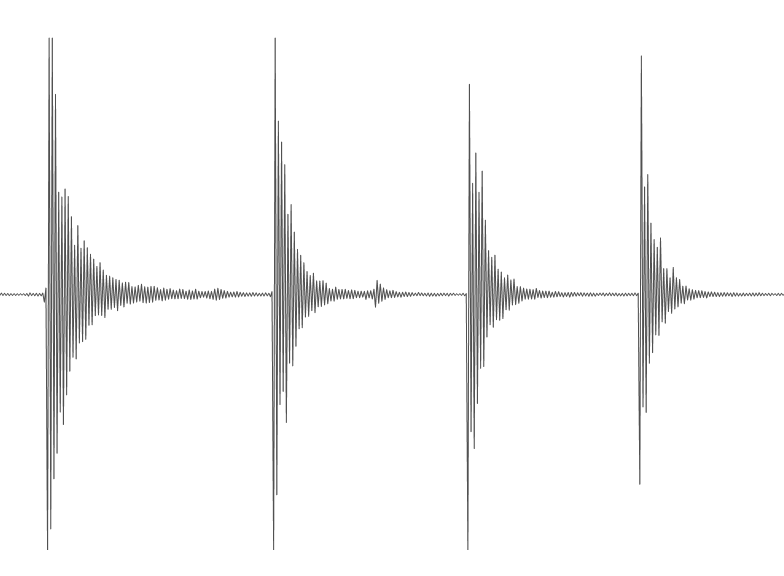
\includegraphics[width=0.5\textwidth]{2013-v3g-02-pall}%
\end{center}
\probend
\bigskip

% Ü8
\setAuthor{Mihkel Rähn}
\setRound{lahtine}
\setYear{2014}
\setNumber{G 1}
\setDifficulty{2}
\setTopic{Dünaamika}

\prob{Kaubarong}
Kaubarongi massiga $m=\SI{5000}{t}$ veab vedur võimsusega $N=\SI{2500}{kW}$. Veerehõõrdetegur rataste ja rööpa vahel on $\mu=\SI{0,002}{}$.\\
\osa Leidke rongi kiirus $v_1$ horisontaalsel teel.\\
\osa Leidke rongi kiirus $v_2$ tõusul üks sentimeeter ühe meetri kohta.\\
Õhutakistusega mitte arvestada.
\probend
\bigskip

% Ü9
\setAuthor{Andreas Valdmann}
\setRound{lahtine}
\setYear{2014}
\setNumber{G 2}
\setDifficulty{2}
\setTopic{Dünaamika}

\prob{Vaakumkahur}
Joonisel on kujutatud niinimetatud vaakumkahur. Laadimiseks pistetakse laskemoonaks olev pall vaakumkahuri toru vasakpoolsest otsast sisse. Seejärel kaetakse toru mõlemad otsad kergestirebeneva õhukindla membraaniga, näiteks fooliumiga, ning pumbatakse torust õhk välja. Nüüd on vaakumkahur laskevalmis. Tulistamiseks purustatakse vasakpoolne membraan, mille tagajärjel hakkab pall toru parempoolse otsa poole sööstma. Piisavalt pika toru korral purustab pall parempoolse membraani ning lendab torust välja. Olgu palli läbimõõt võrdne toru siseläbimõõduga $d=\SI{4,0}{cm}$, palli mass $m=\SI{24}{g}$ ja asugu pall enne tulistamist $l=\SI{150}{cm}$ kaugusel toru parempoolsest otsast. Kui suur on palli kiirus vahetult enne parempoolse membraani läbimist? Õhurõhk on $P_0=\SI{100}{kPa}$. Hõõrdumisega pole tarvis arvestada.
\begin{center}
 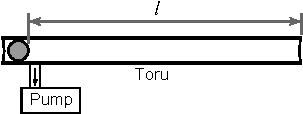
\includegraphics[width=0.75\textwidth]{2014-lahg-02-vaakumkahur.pdf}
\end{center}
\probend
\bigskip

% Ü10
\setAuthor{EFO žürii}
\setRound{lahtine}
\setYear{2016}
\setNumber{G 1}
\setDifficulty{2}
\setTopic{Dünaamika}

\prob{Mängukahur}
\begin{wrapfigure}[6]{r}{0.4\textwidth}
 \vspace{-20pt}
 \begin{center}
 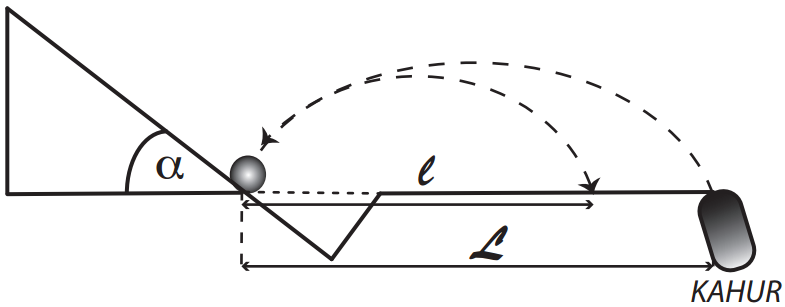
\includegraphics[width=0.4\textwidth]{2016-lahg-01-kaldjoonis}
 \end{center}
 \vspace{-30pt}
\end{wrapfigure}

Mängukahurist tulistatakse kummipall nii, et see põrkab risti kaldpinnaga, kahurist horisontaalkaugusel $L$. Pall põrkab kaldpinnast tagasi kaugusele $l$ (vt joonis). Leidke, kui suur osa energiast neeldus põrkel. Kaldpinna kaldenurk on $\alpha$.
\probend
\bigskip

% Ü11
\setAuthor{Oleg Košik}
\setRound{piirkonnavoor}
\setYear{2016}
\setNumber{G 2}
\setDifficulty{2}
\setTopic{Dünaamika}

\prob{Köievedu}
Eero ja Oleg võistlevad köieveos nii, et kogu võistluse ajal on köis horisontaalne. Eero mass $m_1=\SI{110}{kg}$ ja Olegi mass $m_2=\SI{85}{kg}$. Hõõrdetegur talla ja põranda vahel $\mu=\SI{0,30}{}$ on mõlemal mehel sama. Kumb mees võidab? Millise maksimaalse kiirendusega saab võitja sundida kaotajat liikuma, nii et ta ise veel paigale jääks? Raskuskiirendus $g=\SI{9,8}{m/s^2}$.
\probend
\bigskip

% Ü12
\setAuthor{Moorits Mihkel Muru}
\setRound{lõppvoor}
\setYear{2017}
\setNumber{G 1}
\setDifficulty{2}
\setTopic{Dünaamika}

\prob{Vastlaliug}
\begin{wrapfigure}[5]{r}{0.45\linewidth}
	\vspace{-5pt}
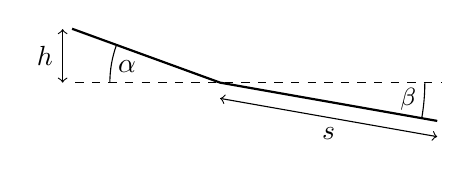
\begin{tikzpicture}[scale=0.4]
% Nõlv
\draw [thick] (0,0) -- (160:5);
\draw [thick] (0,0) -- (-10:7);

% Nurgad
\draw [dashed] (-4.6,0) -- (7,0);
\draw (160:3.5) arc (160:180:3.5) node at (170:3) {\(\alpha\)};
\draw (0:6.5) arc (0:-10:6.5) node at (-5:6) {\small\(\beta\)};

% Suurused
\draw [<->] (-5,0) -- (-5,1.7) node[pos=0.5, left] {\(h\)};
\draw [<->, yshift=-0.5cm] (0,0) -- (-10:7) node[pos=0.5, below] {\(s\)};	
\end{tikzpicture}
%\caption{Künka läbilõige} \label{liug}
\end{wrapfigure}

Juss leidis vastlaliu laskmiseks künka, mille läbilõige koosneb kahest sirglõigust, nagu näha joonisel, edasi on horisontaalne maa. Esimese nõlvaosa kõrgus on \(h=\SI{2}{\meter}\) ja selle kalle \(\alpha=\ang{20}\), teise osa pikkus on \(s=\SI{20}{\meter}\) ja kalle \(\beta=\ang{5}\). Jussi mass koos kelguga on \(m=\SI{47}{\kilogram}\) ja hõõrdetegur lume ja kelgu vahel on \(\mu=\num{0.08}\), raskuskiirendus \(g=\SI{9.8}{\meter\per\second\squared}\). Leidke, kui pikk on Jussi vastlaliug.
\probend
\bigskip

% Ü13
\setAuthor{Kaur Aare Saar}
\setRound{lahtine}
\setYear{2013}
\setNumber{G 3}
\setDifficulty{3}
\setTopic{Dünaamika}

\prob{Alpinist}
Alpinist massiga $m=\SI{75}{kg}$ on kinnitatud elastse nööri külge pikkusega
$L=\SI{6}{m}$. Nööri teine ots on kinnitatud kalju külge. Olles roninud 6 meetri
kõrgusele kinnituskohast, ta kukub. Leidke, kui suur võib olla ülimalt nööri
elastsustegur $k$, teades, et suurim nööri tõmbejõud, mida inimene talub, on
$T=25mg$. Õhutakistust ärge arvestage.
\probend
\bigskip

% Ü14
\setAuthor{Taavi Pungas}
\setRound{piirkonnavoor}
\setYear{2014}
\setNumber{G 5}
\setDifficulty{3}
\setTopic{Dünaamika}

\prob{Langevarjuhüpe}
Juku massiga $m=\SI{60}{\kg}$ ja tema isa Juhan massiga $M=\SI{90}{\kg}$ otsustasid teha langevarjuhüppe. Neile pandi selga ühesugused langevarjud massiga $m_v=\SI{10}{\kg}$ ning nad lükati lennukist välja. Mõlema langevarjud avanesid täielikult ühesugusel kõrgusel $h$, pärast mida saavutasid hüppajad tühise aja jooksul konstantse kiiruse ja liuglesid sellel kiirusel maapinnani. Jukul kulus langevarju avanemisest maapinnani jõudmiseks aega $t=\SI{110}{\s}$. Kui pikk aeg $T$ kulus selleks Juhanil? Langevarjule õhu poolt mõjuv takistusjõud on võrdeline langemiskiiruse ruuduga. Lihtsuse mõttes loeme hüppajatele endile mõjuva õhutakistuse tühiselt väikeseks.
\probend
\bigskip

% Ü15
\setAuthor{Joonas Kalda}
\setRound{piirkonnavoor}
\setYear{2016}
\setNumber{G 4}
\setDifficulty{3}
\setTopic{Dünaamika}

\prob{Kelk}
\begin{wrapfigure}[2]{r}{0.3\textwidth}
	\vspace{-12pt}
	\begin{resizebox}{\linewidth}{!}{
	\begin{tikzpicture}
	\coordinate (C) at (0.7,-0.1);
	\draw (0,0) -- ++(180-15:1.5);
	\draw (0,0) to [out = -15, in = 180] (C);
	\draw (C) to ++(0:1.5);
	\draw (180-15:1.5) -- ++(-15:0.2) -- ++(90-15:0.1) -- ++(180-15:0.2) -- (180-15:1.5);
	\end{tikzpicture}}
	\end{resizebox}
\end{wrapfigure}

Juku tahab kelguga ületada jääga kaetud jõge. Ta stardib lumega kaetud kaldalt, mis on horisondiga $\alpha = 15^{\circ}$ nurga all. Jõe laius $l = \SI{10}{m}$, kelgu ja lume vaheline hõõrdetegur $\mu_1 = \SI{0.20}{}$, kelgu ja jää vaheline hõõrdetegur $\mu_2 = \SI{0.10}{}$. Kui kõrgele veepinnast peab kallas ulatuma, et Juku libiseks teise kaldani?
\probend
\bigskip

% Ü16
\setAuthor{Eero Vaher}
\setRound{lõppvoor}
\setYear{2016}
\setNumber{G 2}
\setDifficulty{3}
\setTopic{Dünaamika}

\prob{Pidurdus}
Auto sõidab teel, mille kõrguse muut teepikkuse kohta on $k=\frac{1}{30}$. Ühesuguse algkiiruse ning pidurdusjõu korral jääb auto ülesmäge liikudes seisma vahemaa $s_1=\SI{25}{m}$ jooksul, allamäge liikudes aga vahemaa $s_2=\SI{30}{m}$ jooksul. Mis on auto algkiiruse $v$ väärtus? Raskuskiirendus $g=\SI{9.8}{\meter\per\second\squared}$.
\probend
\bigskip

% Ü17
\setAuthor{Hans Daniel Kaimre}
\setRound{lõppvoor}
\setYear{2016}
\setNumber{G 3}
\setDifficulty{3}
\setTopic{Dünaamika}

\prob{Kahurikuul}
Juku arvutas koolitunnis ülivõimsast kahurist otse üles lastud kuuli maksimaalseks kõrguseks $H=\SI{400}{\km}$. Ta ei arvestanud aga seda, et sellistel kõrgustel gravitatsioonivälja muutus on juba märkimisväärne ning ei saa eeldada, et raskusjõud on konstantne. Leidke, kui kõrgele kuul tegelikult lendaks. Maa raadius $R=\SI{6400}{\km}$. Õhutakistusega mitte arvestada.
\probend
\bigskip

% Ü18
\setAuthor{Andreas Valdmann}
\setRound{piirkonnavoor}
\setYear{2017}
\setNumber{G 3}
\setDifficulty{3}
\setTopic{Dünaamika}

\prob{Pendel}
Nöörist ja koormisest koosnev pendel võngub nii, et amplituudasendis on nööri ja vertikaalsihi vaheline nurk $\alpha=\ang{60}$. Mitu korda erinevad võnkumise käigus suurim ja vähim pinge nööris?
\probend
\bigskip

% Ü19
\setAuthor{Jonatan Kalmus}
\setRound{lõppvoor}
\setYear{2017}
\setNumber{G 2}
\setDifficulty{3}
\setTopic{Dünaamika}

\prob{Mäenõlv}
Kui suure maksimaalse kaldenurgaga $\alpha$ mäenõlvast on võimalik jalgrattaga konstantse kiirusega üles sõita? Ratturi mass on $m$, jalgratta mass $M$, pedaali vända pikkus $r_1$, eesmise hammasratta raadius $r_2$, tagumise hammasratta raadius $r_3$, ratta raadius $r_4$. Eeldada, et ratturi massikese püsib sõitmise käigus ratta suhtes paigal ja sõitja kannab kogu oma kehakaalu vajuval pedaalil. Hõõrdetegur pinna ja ratta vahel on piisavalt suur libisemise vältimiseks. Mehaanilise hõõrdumisega jõuülekandes mitte arvestada ning veerehõõrdejõu võib lugeda tühiseks. Eeldada, et jalgratta keskmine kiirus püsib ligikaudselt konstante ja kiiruse suhteline muutus veerand väntamisperioodi jooksul on tühiselt väike.\\
\emph{Märkus.} Ülesande teksti on olümpiaadil esineva versiooniga võrreldes kohandatud.
\probend
\bigskip

% Ü20
\setAuthor{Kristian Kuppart}
\setRound{lahtine}
\setYear{2011}
\setNumber{G 3}
\setDifficulty{4}
\setTopic{Dünaamika}

\prob{Veoauto}
Veoauto kastis kõrgusega $H$ on vedelik, mille pinna kõrgus kasti põhjast on 
$h$, kusjuures $h > \frac{H}{2}$. Kui suure kiirendusega $a$ saab veoauto 
liikuda, ilma et vedelik kastist välja voolaks? Veoauto kasti pikkus on $L$.\\
\textit{Märkus.} Auto kiirendab sujuvalt ning tänu sellele vedelik võnkuma ei hakka.
\probend
\bigskip

% Ü21
\setAuthor{Andreas Valdmann}
\setRound{piirkonnavoor}
\setYear{2012}
\setNumber{G 5}
\setDifficulty{4}
\setTopic{Dünaamika}

\prob{Surmasõlm}
\begin{wrapfigure}{r}{42mm}%
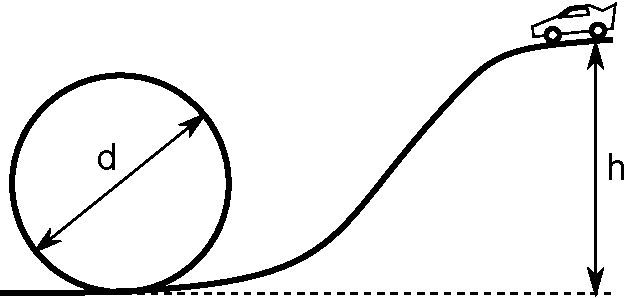
\includegraphics[width=\linewidth]{2012-v2g-05-silmus}%
\end{wrapfigure}
Mudelauto rada on kujutatud joonisel: auto alustab kaldtee tipus seisvast
asendist, kogub laskumisel kiirust ja teeb silmuses surmasõlme. Mis on
minimaalne kõrgus $h$, et auto silmuse läbimisel alla ei kukuks? Silmuse
läbimõõt on $d$. Hõõrdumisega arvestada ei ole vaja.
\probend
\bigskip

% Ü22
\setAuthor{Mihkel Kree}
\setRound{lõppvoor}
\setYear{2012}
\setNumber{G 2}
\setDifficulty{4}
\setTopic{Dünaamika}

\prob{Veejuga}
Pildil on foto horisontaalsest torust väljuva veejoaga ning teljestik, mille
väikseim jaotis on võrdne veejoa läbimõõduga selle algkõrgusel. Ühtlase
kiirusega voolava veejoa alla pandud mõõteklaas ruumalaga
$V=\SI{150}{cm^3}$ täitus ajaga $t=\SI{5}{min}$. Leidke
toru siseläbimõõt.
\begin{center}
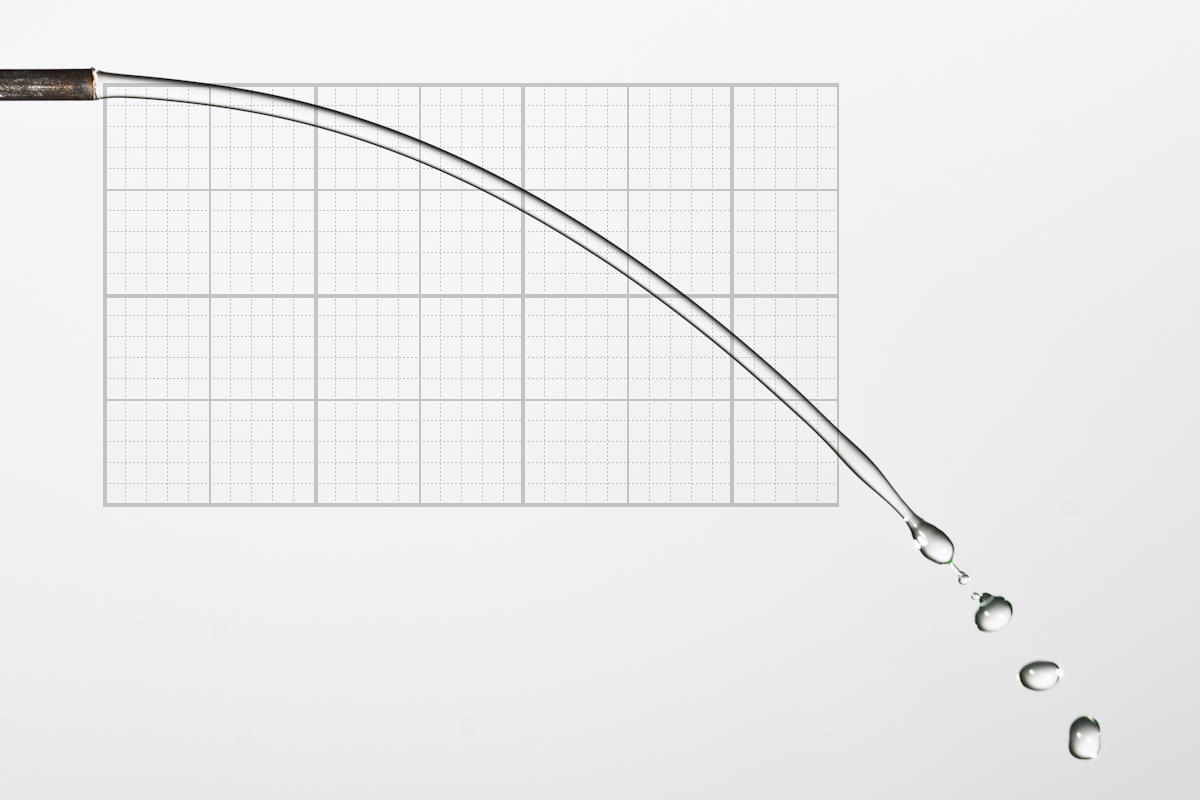
\includegraphics[width=0.7\linewidth]{2012-v3g-02-jet}%
\end{center}
\probend
\bigskip

% Ü23
\setAuthor{Aigar Vaigu}
\setRound{piirkonnavoor}
\setYear{2016}
\setNumber{G 6}
\setDifficulty{4}
\setTopic{Dünaamika}

\prob{Lasketiir}
Siselasketiirus tulistatakse vintpüssist, mille kuuli kiirus $v=\SI{320}{m/s}$, kaugusel $s=\SI{30}{m}$ olevat märklauda. Laskur sihib püssiga samal kõrgusel olevat märki ja tabab seda otse kümnesse. Hinnake, kui kaugele sihtmärgist satuks kuul, kui relva enne laskmist keerata ümber sihtimistelje 180 kraadi? Õhutakistusega mitte arvestada.
\probend
\bigskip

% Ü24
\setAuthor{Kaur Aare Saar}
\setRound{lõppvoor}
\setYear{2016}
\setNumber{G 4}
\setDifficulty{4}
\setTopic{Dünaamika}

\prob{Silinder}
Silinder massiga $m$ ja raadiusega $R$ libiseb tasapinnal kiirusega $v$ ja nurkkiirusega $\omega$. Kui libisemine on lõppenud, liigub silinder kiirusega $v$ esialgsega vastupidises suunas. Leidke silindri esialgne nurkkiirus.

\begin{center}
	\begin{resizebox}{0.35\linewidth}{!}{
			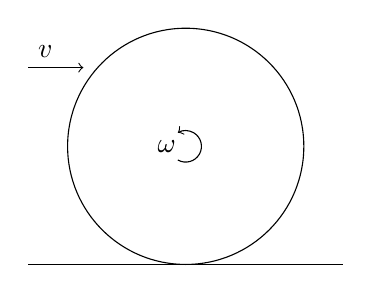
\begin{tikzpicture}
			\draw (0,2.5) node[anchor=south west] {$v$};
			\draw[->] (0,2.5) -- ++(0:0.7);
			\draw (0,0) --(4,0);
			\draw (2,1.5) circle (1.5);
			\draw [->] (2,1.5) node[anchor = east] {$\omega$} ++(-120:0.2) arc (-120:120:0.2);
			\end{tikzpicture}}
	\end{resizebox}
\end{center}
\probend
\bigskip

% Ü25
\setAuthor{Jonatan Kalmus}
\setRound{piirkonnavoor}
\setYear{2018}
\setNumber{G 5}
\setDifficulty{4}
\setTopic{Dünaamika}

\prob{Veok ringteel}
Veok sõidab ringteel kõverusraadiusega $R$ ühtlase kiirusega. Leida veoki maksimaalne võimalik kiirus, eeldusel et hõõrdetegur on piisavalt suur libisemise vältimiseks. Veoki massikeskme kõrgus maapinnast on $h$ ja veoki laius $l$. Raskuskiirendus on $g$.
\probend
\bigskip

% Ü26
\setAuthor{Ants Remm}
\setRound{lahtine}
\setYear{2012}
\setNumber{G 6}
\setDifficulty{5}
\setTopic{Dünaamika}

\prob{Kloori molekul}
Kloori molekul, mis liigub kiirusega $v = \SI{600}{m/s}$, neelab
footoni lainepikkusega $\lambda = \SI{350}{nm}$ ning jaguneb kaheks aatomiks.
Ühe aatomi kiiruseks
mõõdetakse $ u = \SI{1600}{m/s}$, mis on risti molekuli esialgse
kiirusega. Leidke kloori molekuli seoseenergia, kui kõik osakesed olid
minimaalse siseenergiaga seisundis. Plancki konstant on $h =
\SI{6,6e-34}{J.s}$, valguse kiirus on $c = \SI{3,0e8}{m/s}$, kloori aatomnumber on 35 ning Avogadro arv on $N_A
= \SI{6,0e23}{\text{mol}^{-1}}$. Footoni energia avaldub valemiga $E =
\frac{h c}{\lambda}$. Eeldada, et footoni impulss on tühine võrreldes Kloori impulsiga.
\probend
\bigskip

% Ü27
\setAuthor{Andres Põldaru}
\setRound{lahtine}
\setYear{2014}
\setNumber{G 5}
\setDifficulty{5}
\setTopic{Dünaamika}

\prob{Kiik}
Kiige ühe otsa peal kaugusel $l_1$ kiige pöörlemisteljest asub mass $m_1$. Kiige teise otsa peale, mis on pöörlemisteljest kaugusel $l_2$, kukub kõrguselt $h$ mass $m_2$. Kokkupõrge on absoluutselt mitteelastne ning kiik on kokkupõrkehetkel horisontaalne. Kiige mass on väga väike ja sellega ei pea arvestama. Kui kiiresti liigub esimene mass vahetult pärast kokkupõrget?
\probend
\bigskip

% Ü28
\setAuthor{Jaan Toots}
\setRound{lahtine}
\setYear{2015}
\setNumber{G 6}
\setDifficulty{5}
\setTopic{Dünaamika}

\prob{Vesiniku ioniseerimine}
Kui suur on vähim vesiniku aatomit ioniseerida suutva vaba prootoni kineetiline energia $K_0$? Eeldage, et elektron on vesiniku aatomis paigal ning elektromagnetiline vastasmõju aatomi tuuma ja vaba prootoni vahel on tühine. Vesiniku seoseenergia $E_0 = \SI{13.6}{\electronvolt}$, prootoni mass $m_p=\SI{1.67e-27}{kg}$ ja elektroni mass $m_e=\SI{9.11e-31}{kg}$.
\probend
\bigskip

% Ü29
\setAuthor{Kristian Kuppart}
\setRound{piirkonnavoor}
\setYear{2015}
\setNumber{G 5}
\setDifficulty{5}
\setTopic{Dünaamika}

\prob{Veetoru}
\begin{wrapfigure}[5]{r}{0.18\textwidth}
 \vspace{-30pt}
 \begin{center}
 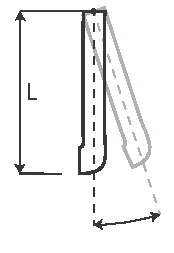
\includegraphics[width=0.18\textwidth]{2015-v2g-05-toru}
 \end{center}
\end{wrapfigure}
Veetoru pikkusega $L$ on kinnitatud seina külge nii, et see saab vertikaaltasandis vabalt pöörelda. Veetoru mass koos seda täitva veega on $M$. Toru ots ristlõikepindalaga $S$ on ülejäänud toruga võrreldes \num{90} kraadi pööratud (vt joonist) ning sellest voolab välja vesi kiirusega $v$ ja tihedusega $\rho$. Kui suure nurga all vertikaali suhtes paikneb toru telg? Raskuskiirenduse väärtus on $g$.
\probend
\bigskip

% Ü30
\setAuthor{Mihkel Kree}
\setRound{piirkonnavoor}
\setYear{2015}
\setNumber{G 6}
\setDifficulty{5}
\setTopic{Dünaamika}

\prob{Põrge}
\begin{wrapfigure}[7]{r}{0.22\textwidth}
 \vspace{-20pt}
 \begin{center}
 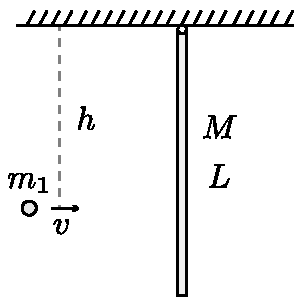
\includegraphics[width=0.22\textwidth]{2015-v2g-06-porgejoonis}
 \end{center}
 %\vspace{-30pt}
\end{wrapfigure}

Algselt paigal olev rippuv varras massiga $M$ ning pikkusega $L$ on fikseeritud ülemisest otsast vabalt pöörleva kinnitusega. Varda inertsimoment otspunkti suhtes on $I=\frac{1}{3}ML^2$. Teraspall massiga $m_1$ lendab vastu varrast ning tabab seda kaugusel $h$ riputuspunktist. Põrge on elastne, st soojuskadudeta. Huvitaval kombel jääb teraskuul pärast põrget hetkeks paigale ning hakkab seejärel vertikaalselt alla langema. Leidke kauguse $h$ väärtus, mille korral niisugune seismajäämine võimalik on.
\probend
\bigskip

% Ü31
\setAuthor{Ardi Loot}
\setRound{lahtine}
\setYear{2016}
\setNumber{G 6}
\setDifficulty{5}
\setTopic{Dünaamika}

\prob{Rattur}
Rattur massiga $m=\SI{100}{kg}$ sõidab ilma väntamata alla mäenõlvalt langemisnurgaga
$\theta_{1}=\ang{4.8}$ (nurk horisondi ja mäenõlva vahel)
ja märkab, et piisavalt pika nõlva korral on tema lõppkiiruseks $v_{1}=\SI{50}{km/h}$.
Kaks korda väiksema nõlva korral $(\theta_{2}=\ang{2.4})$
on ratturi lõppkiirus aga $\Delta v=\SI{15}{km/h}$ võrra väiksem.
Leidke, kui suur peab olema ratturi väntamise võimsus, et horisontaalsel
teel hoida kiirust $v=\SI{20}{km/h}.$ Kui suur osa võimsusest kulub
tuuletakistuse ületamiseks? Eeldage, et tegemist on tuulevaikse ilmaga
ja raskuskiirendus $g=\SI{9.8}{m/s^{2}}$. 

\emph{Märkus.} Arvestada tuleks nii kiirusest sõltumatu hõõrdejõuga kui ka tuuletakistusega,
mis on võrdeline kiiruse ruuduga.
\probend
\bigskip

% Ü32
\setAuthor{Rasmus Kisel}
\setRound{piirkonnavoor}
\setYear{2017}
\setNumber{G 7}
\setDifficulty{5}
\setTopic{Dünaamika}

\prob{Kaks kuuli ja vedru}
Vedru erinevatesse otstesse on kinnitatud väikesed kuulid, millest ühe mass on $M$ ning teise oma tundmatu. Kogu süsteem pannakse pöörlema nii, et tundmatu massi kaugus pöörlemiskeskmest on võrdne vedru esialgse pikkusega. Mis on selle pöörlemise periood, kui vedru jäikus on $k$? Vedru mass on võrreldes kuulide massidega tühine.
\probend
\bigskip

% Ü33
\setAuthor{Moorits Mihkel Muru}
\setRound{lõppvoor}
\setYear{2017}
\setNumber{G 5}
\setDifficulty{5}
\setTopic{Dünaamika}

\prob{Reisirong}
Reisirong sõidab mööda raudtee ringjoone kaarekujulist lõiku ühtlaselt aeglustudes. Lõigu pikkus on $s$ ja rongil kulub selle läbimiseks aeg $t$. Pärast selle lõigu läbimist on rongi liikumise suund muutunud nurga $\varphi$ võrra ja lõigu alguses oli rongi kiirus $\alpha$ korda suurem, kui see on lõigu lõpus. Leidke seos rongis istuva reisija massi $m$ ja tema kaalu $P$ vahel, kui reisirong on parajasti selle lõigu keskpunktis. Leidke reisija mass, kui $P=\SI{840}{\newton}$, $s=\SI{1.5}{\kilo\meter}$, $t=\SI{60}{\second}$, $\alpha=\num{1.5}$, $\varphi=\ang{60}$ ja $g=\SI{9.8}{\meter\per\second\squared}$.
\probend
\bigskip

% Ü34
\setAuthor{Hans Daniel Kaimre}
\setRound{lõppvoor}
\setYear{2018}
\setNumber{G 4}
\setDifficulty{5}
\setTopic{Dünaamika}

\prob{Kaheosaline pendel}
\begin{wrapfigure}[10]{r}{0.4\textwidth}
\vspace{-5pt}
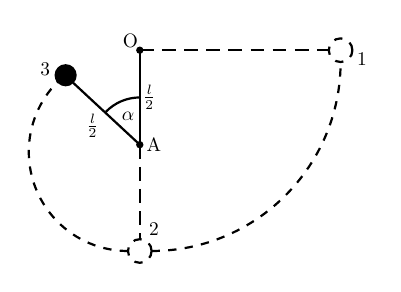
\begin{tikzpicture}[thick,scale=0.6, every node/.style={scale=0.7}]

 % Def. koordinaadid
 \coordinate (O) at (0,0) ;
 \coordinate (1) at (4,0) ;
 \coordinate (A) at (0,-2) ;
 \coordinate (2) at (0,-4);
 \coordinate (3) at (-1.41,-0.69);

 % Jooned, t2pid
 \draw[dash pattern=on5pt off3pt] (O) -- (1);
 \draw[dash pattern=on5pt off3pt] (A) -- (2);
 \draw[thick,dashed] (4.25,0) circle (0.25cm);
 \draw[thick,dashed] (0,-4.25) circle (0.25cm);
 \draw[thick] (O) -- (A);
 \draw[thick] (A) -- (3);
 \filldraw [black] (A) circle (1.5pt);
 \filldraw [black] (O) circle (1.5pt);
 \filldraw [black] (-1.57,-0.53) circle (6pt);
 
 

 % Nurgad ja punktid
 \draw (0,-1) arc (90:136:1);
 \draw[thick, dashed] (0.25,-4.25) arc (270:360:4);
 \draw[thick, dashed] (-0.25,-4.25) arc (270:135:2.1);
 \node[] at (-0.25,-1.4) {$\alpha$};
 \node[] at (4.7,-0.2) {$1$};
 \node[] at (0.3,-3.8) {$2$};
 \node[] at (-2.0,-0.4) {$3$};
 \node[] at (-0.2,0.2) {O};
 \node[] at (0.3,-2) {A};
 \node[] at (0.2,-1) {$\frac{l}{2}$};
 \node[] at (-1,-1.6) {$\frac{l}{2}$};
\end{tikzpicture}
\end{wrapfigure}

Punktis O kinnitatud niidi pikkusega $l$ otsas ripub väike kuulike. Kuulike viiakse kõrvale ja vabastatakse tõuketa asendist 1. Kuuli jõudes asendisse 2, kohtab niit joonise tasandiga risti olevat varrast punktis A, mis asub punktist O kaugusel $l/2$ sellega samal vertikaalil. Leida, millise nurga $\alpha$ väärtuse korral niidi pinge $T=0$ (asend 3). Õhutakistust ja hõõrdumist vardal arvestama ei pea.
\probend
\bigskip

% Ü35
\setAuthor{Hans Daniel Kaimre}
\setRound{piirkonnavoor}
\setYear{2016}
\setNumber{G 8}
\setDifficulty{6}
\setTopic{Dünaamika}

\prob{Veerev pall}
\begin{wrapfigure}{r}{0.3\textwidth}
	\vspace{-15pt}
	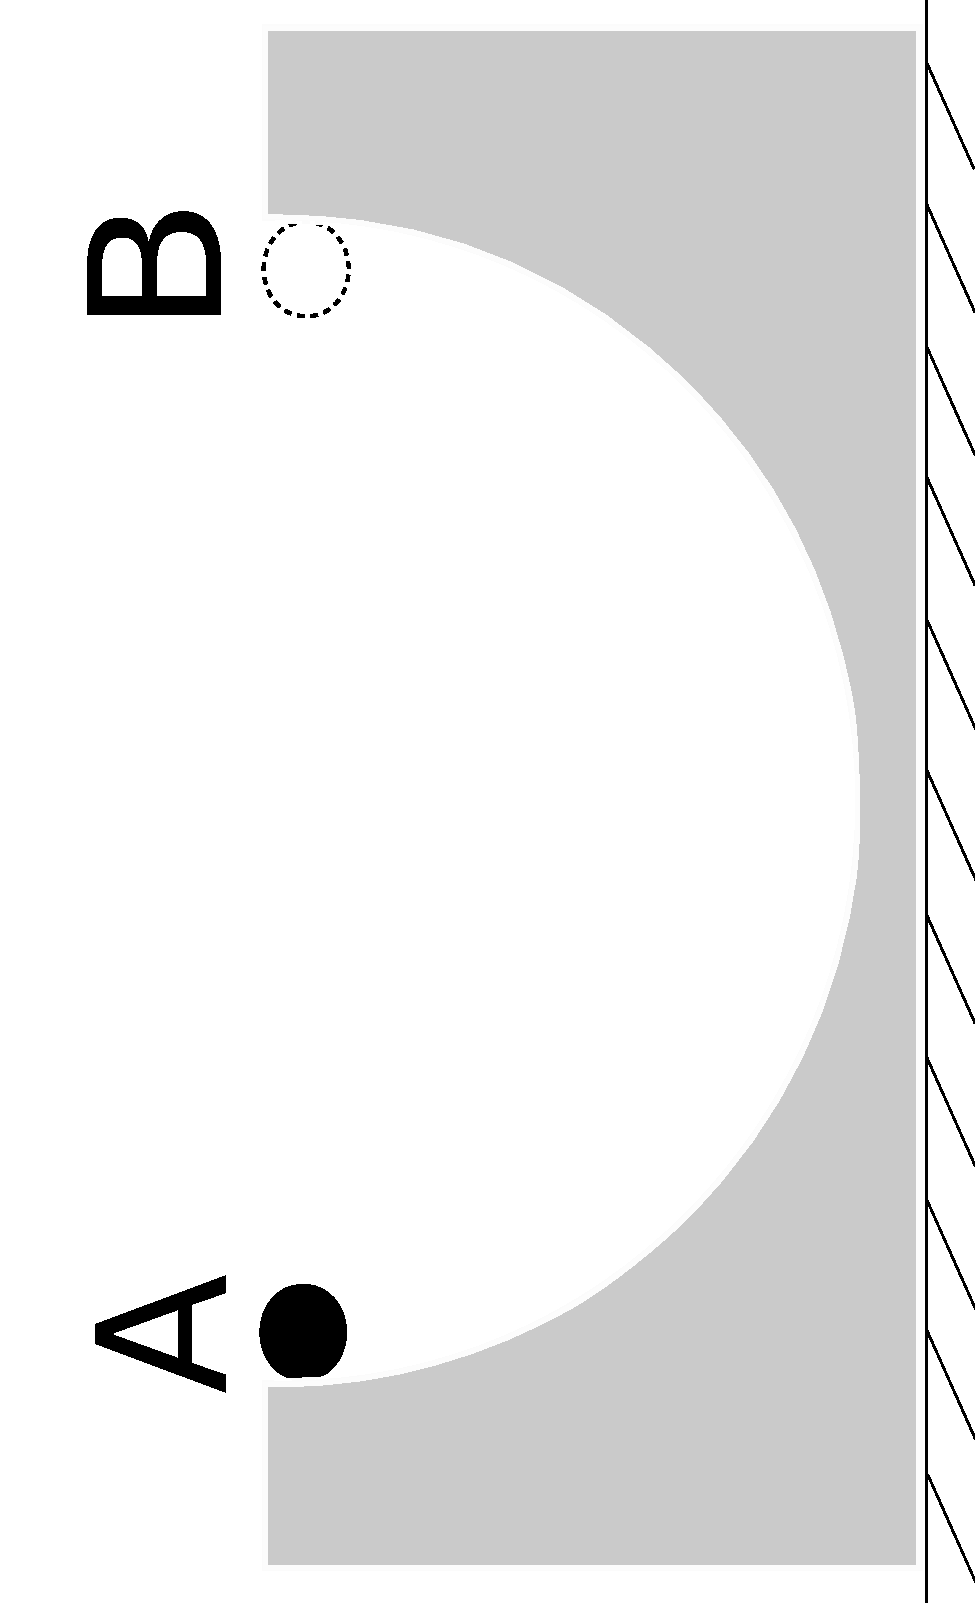
\includegraphics[angle=-90,origin=c,width=0.3\textwidth]{2016-v2g-08-halfpipe.pdf}
\end{wrapfigure}
Klotsist on välja lõigatud poolsilindrikujuline tükk raadiusega $R$. Klots seisab siledal hõõrdevabal horisontaalsel pinnal (vaata joonist). Klotsi mass on $M$. Punktist A lükatakse liikuma mööda silindrikujulise väljalõike pinda väike pall raadiusega $r$ ning massiga $m$. Kui palju on nihkunud klots hetkeks, mil pall jõuab punkti B?
\probend
\bigskip

% Ü36
\setAuthor{Tanel Kiis}
\setRound{lahtine}
\setYear{2012}
\setNumber{G 7}
\setDifficulty{7}
\setTopic{Dünaamika}

\prob{Pidurdamine}
Keha massiga $M$ kukub vabalt raskusjõu toimel kiirendusega~$g$. Tema
kiirust proovitakse muuta, tulistades maalt otse üles iga $t$ sekundi tagant
väikeseid kuulikesi massiga~$m$, mis põrkavad elastselt otse tagasi.
Kui suur peab olema kuulikeste kiirus~$u$, et pärast iga põrget oleks langeva
keha kiirus üks ja seesama~$v$? Võib eeldada, et väikeste kuulikeste kiiruse muut raskusjõu toimel on
tühine ja $m\ll M$.
\probend
\bigskip

% Ü37
\setAuthor{Madis Ollikainen}
\setRound{piirkonnavoor}
\setYear{2012}
\setNumber{G 9}
\setDifficulty{7}
\setTopic{Dünaamika}

\prob{Robin Hood}
Robin Hood on täpsuslaskmisvõistlustel, kus tal tuleb tabada märklauda, mis asub
$L=\SI{200}{m}$ kaugusel. Millise nurga $\alpha$ all horisontaalsihi suhtes
peab Robin vibust laskma, et tabada täpselt märklaua keskpunkti? Vibu vinnamisel
teeb ta tööd $A=\SI{500}{J}$ ning vibu kasutegur on $\eta=0,17$. Noole mass on
$m=\SI{54}{g}$ ja see lastakse lendu märklaua keskpunktist $h=\SI{70}{cm}$ võrra
kõrgemalt. Õhutakistusega ärge arvestage. Raskuskiirenduseks lugege
$g=\SI{9,8}{m/s^2}$.
\probend
\bigskip

% Ü38
\setAuthor{Mihkel Rähn}
\setRound{lõppvoor}
\setYear{2014}
\setNumber{G 7}
\setDifficulty{7}
\setTopic{Dünaamika}

\prob{Sportauto}
Leidke esirattaveolise sõiduauto maksimaalne kiirendus. Auto mass on $m$, esi- ja tagarataste telgede vahe $b$, masskeskme kõrgus $h$ ning masskeskme horisontaalne kaugus tagateljest $s$. Hõõrdetegur rataste ja maa vahel on $\mu$.
\probend
\bigskip

% Ü39
\setAuthor{Kaur Aare Saar}
\setRound{lahtine}
\setYear{2015}
\setNumber{G 8}
\setDifficulty{7}
\setTopic{Dünaamika}

\prob{Latt}
Pikka horisontaaltasapinnal lebavat latti lükatakse ühest otsast muutumatu kiirusega ning risti latiga. Kui kaugel sellest lati otsast asub lati pöörlemistelg? Lati pikkus on $L$. Hõõrdetegur lati ja tasapinna vahel on kõikjal ühesugune.
\probend
\bigskip

% Ü40
\setAuthor{Tanel Kiis}
\setRound{piirkonnavoor}
\setYear{2013}
\setNumber{G 9}
\setDifficulty{8}
\setTopic{Dünaamika}

\prob{Õõnes kera}
Jukul on rauast kera
($\varrho_\mathrm{Fe}=\SI{7,9}{\gram\per\centi\meter\cubed}$) raadiusega
$r=\SI{10}{\centi\meter}$ ja massiga $m=\SI{30}{\kilo\gram}$. Juku teab, et kera
sees on sfääriline õõnsus, mille keskpunkti kaugust $d$ kera keskpunktist ta üritab
leida. Selleks riputas ta kuuli kaks korda nööri otsa rippuma, kasutades
riputuskohtadeks kera vastaspunkte. Ühel korral moodustas neid kinnituspunkte
ühendav telg horisondiga nurga $\alpha=\ang{60}$, teisel korral aga nurga
$\beta=\ang{45}$. Leidke $d$.
\probend
\bigskip

% Ü41
\setAuthor{Andreas Valdmann}
\setRound{lõppvoor}
\setYear{2013}
\setNumber{G 9}
\setDifficulty{8}
\setTopic{Dünaamika}

\prob{Jalgpallurid}
Kaks jalgpallurit proovisid trikilööki, kus kaks palli õhus kokku põrkavad.
Jalgpallurid seisid teineteisest $d = \SI{20}{m}$ kaugusel ja andsid samal ajahetkel
sooritatud löögiga kumbki oma pallile algkiiruse $v = \SI{15}{m/s}$. Mis piirkonnas võisid pallid lennul kokku põrgata?
Vastuseks tehke pealtvaates joonis, kuhu on kantud jalgpallurite
asukohad ja kõikvõimalike kokkupõrkepunktide piirkond. Esitage ka selle
piirkonna mõõdud. Võimalike kokkupõrkepunktide kõrgust maapinnast pole
vaja eraldi välja arvutada ega joonisele kanda. Raskuskiirendus
on $g = \SI{9,8}{m/s^2}$.
\probend
\newpage

\bigskip

% Ü42
\setAuthor{Andres Põldaru}
\setRound{lahtine}
\setYear{2015}
\setNumber{G 9}
\setDifficulty{8}
\setTopic{Dünaamika}

\prob{Mutrivõti}
Kui suur peab olema reguleeritava mutrivõtme keerete arv pikkusühiku kohta $n$, et mutreid saaks kõvasti kinni keerata? Hõõrdetegur kokkupuutepindade vahel on $\mu$ ja raadius reguleerija teljest kokkupuutepinnani on $r$.
\begin{center}%
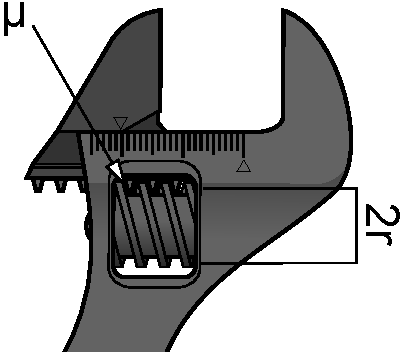
\includegraphics[width=0.4\linewidth]{2015-lahg-09-mutriv6ti_joonis}%
\end{center}
\probend
\bigskip

% Ü43
\setAuthor{Taavet Kalda}
\setRound{lahtine}
\setYear{2017}
\setNumber{G 8}
\setDifficulty{8}
\setTopic{Dünaamika}

\prob{Plokid}
Joonisel on kujutatud kahest plokist ja kolmest raskusest, massidega $m_1$, $m_2$ ja $M$ koosnevat süsteemi. Nöörid on venimatud ning nööride ja plokkide massid on tühised võrreldes raskuste massidega. Hõõre ploki ja nööri vahel on tühiselt väike. Missugune peaks olema $M$ väärtus selleks, et $M$ jääks esialgu paigale, kui süsteem lahti lasta?

\begin{center}
	\vspace{-10pt}
	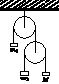
\includegraphics[width = 0.3\linewidth] {2017-lahg-08-double_pulleys_img.pdf}
\end{center}
\probend
\bigskip

% Ü44
\setAuthor{Jaan Kalda}
\setRound{lahtine}
\setYear{2017}
\setNumber{G 9}
\setDifficulty{8}
\setTopic{Dünaamika}

\prob{Mänguauto}
Mänguauto telgede vaheline kaugus on $L$ ning massikese asub võrdsel kaugusel telgedest kõrgusel $h$ horisontaalpinnast. Auto esimesed rattad saavad vabalt pöörelda ja on tühise massiga, tagumised rattad on aga jäigalt kinni kiilunud ega pöörle üldse. Auto lebab horisontaalsel pinnal, rataste ja horisontaalpinna vaheline hõõrdetegur on $\mu$, raskuskiirendus on $g$.

Horisontaalpinda hakatakse liigutama kõrge sagedusega horisontaalselt edasi-tagasi: ühe poolperioodi jooksul on pinna kiirusvektor suunatud auto tagaratastelt esiratastele ning teise poolperioodi jooksul on see vastassuunaline; mõlema poolperioodi jooksul püsib kiiruse moodul konstantsena; võngutamisel liigutatakse pinda nii kiiresti, et auto libiseb pinna suhtes kogu aeg kas ühes või teises suunas. Millise keskmise kiirendusega hakkab liikuma auto?
\probend
\bigskip

% Ü45
\setAuthor{Jaan Kalda}
\setRound{lahtine}
\setYear{2012}
\setNumber{G 10}
\setDifficulty{9}
\setTopic{Dünaamika}

\prob{Killud}
Savikuulike massiga \SI{10}{g} kukkus vertikaalselt alla siledale horisontaalsele
põrandale ja läks kolmeks killuks.
Killud lendasid laiali ja peatusid punktides, mis on näidatud juuresoleval
joonisel
(ülaltvaade, ristiga on märgitud kukkumiskoht). Määrake kildude massid.
Joonisel (lisalehel)
võib teha lisakonstruktsioone ja mõõtmisi.
Võite lugeda, et killud hakkasid kohe pärast kukkumist üles põrkumata libisema,
õhuhõõre on tühine ja liugehõõrdetegur ei sõltu kiirusest.
\begin{center}
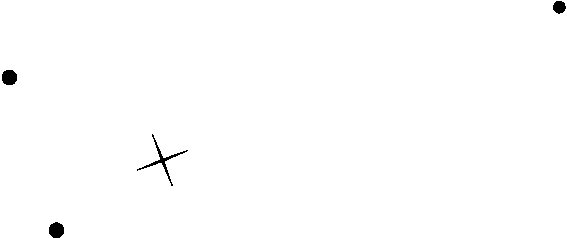
\includegraphics[width=0.8\linewidth]{2012-lahg-10-killud}
\end{center}
\probend
\newpage

\bigskip

% Ü46
\setAuthor{Roland Matt}
\setRound{lõppvoor}
\setYear{2012}
\setNumber{G 8}
\setDifficulty{9}
\setTopic{Dünaamika}

\prob{Liivakell}
Uurime liivakella mudelit. Liivakell koosneb silindrilisest torust pikkusega
$L$, mis on keskelt eraldatud ühtlaselt aukudega läbistatud plaadiga, millest
liiv saab läbi voolata. Heas lähenduses ei sõltu liiva aukude läbimise
masskiirus $w$ ülemises anumas olevast liivahulgast. Liivakell asetatakse
kaalule töörežiimis (kui liiv voolab) ja siis, kui kogu liiv on alla voolanud.
Milline on kaalunäitude vahe? Liiva tihedus on $\rho$ ja liivakella
ristlõikepindala on $S$. Eeldage, et hetkel kukkuva liiva mass on tühine
võrreldes liiva kogumassiga.
\probend
\bigskip

% Ü47
\setAuthor{Jaan Kalda}
\setRound{lõppvoor}
\setYear{2014}
\setNumber{G 8}
\setDifficulty{9}
\setTopic{Dünaamika}

\prob{Silindrilised anumad}
\begin{wrapfigure}{r}{0.07\textwidth}%
\vspace{-15pt}
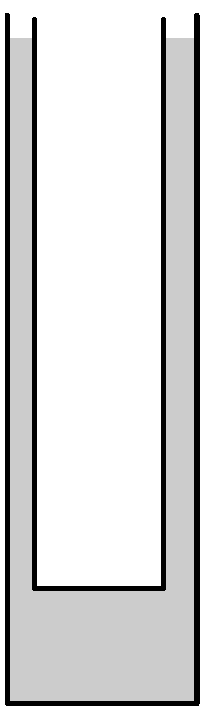
\includegraphics[width=1\linewidth]{2014-v3g-08-cylinders}
\end{wrapfigure}

Silindriline anum siseraadiusega $R = \SI{30}{mm}$ on täidetud veega. Teine tühi silindriline anum raadiusega $r =\SI{25}{mm}$, mille mass on tühiselt väike, on surutud koaksiaalselt suurema silindri sisse nii, et selle vettesukeldunud osa pikkus $L = \SI{300}{mm}$ (vt joonist). Leidke sisemise silindri kiirendus vahetult pärast seda, kui see vabaks lastakse. Vee pindpinevuse ning viskoossusega arvestada pole tarvis.
\probend
\bigskip

% Ü48
\setAuthor{Mihkel Kree}
\setRound{lõppvoor}
\setYear{2015}
\setNumber{G 8}
\setDifficulty{9}
\setTopic{Dünaamika}

\prob{Vedru}
Kasti sees on vedru külge riputatud koormis. Nii kast kui koormis on massiga $m$. Vedru mass on tühiselt väike ning selle jäikustegur on $k$. Kastil lastakse kõrguselt $h$ vabalt maha kukkuda nii, et langemise ajal on koormis tasakaaluolekus. Kokkupõrkel pehme pinnaga jääb kast hetkeliselt paigale. Kast on piisavalt kõrge selleks, et koormis vastu kasti ei põrkaks. Vedrut ei suruta ühelgi hetkel täielikult kokku.\\
\osa Milline on vähim kõrgus $h_\text{m}$, millelt kukkudes hüppab kast tagasi üles?\\
\osa Kastil lasti kukkuda punktis a) leitud algkõrguselt $h\approx h_\text{m}$. Kui pika ajavahemiku $t$ veedab kast maapinnal enne üles kerkimist? 

\emph{Märkus.} Pange tähele, et vabalangemises olev koormis on kaaluta olekus ning seetõttu on vedru langemise ajal välja venitamata. Maapinnale jõudes pole koormis enam tasakaaluasendis ning hakkab seetõttu uue tasakaaluasendi ümber võnkuma nurksagedusega $\omega =\sqrt{\frac{k}{m}}$.
\probend
\bigskip

% Ü49
\setAuthor{Jaan Kalda}
\setRound{lahtine}
\setYear{2017}
\setNumber{G 10}
\setDifficulty{9}
\setTopic{Dünaamika}

\prob{Vardad}
\begin{wrapfigure}[7]{r}{0.4\textwidth}
	\vspace{-10pt}
	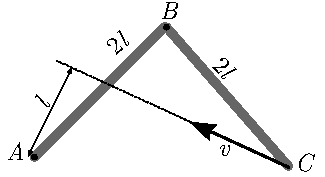
\includegraphics[width = 0.4\textwidth] {2017-lahg-10-delta.pdf}
\end{wrapfigure}

Juuresoleval joonisel on kujutatud kahest vardast pikkusega $2l$ koostatud \v sarniirne konstruktsioon. Ühe varda otspunkt on fikseeritud liikumatuna punkti $A$ ning teise varda otspunkt $C$ liigub konstantse kiirusega $v$ piki sihti, mis möödub punktist $A$ kaugusel $l$. Leidke varraste ühenduspunkti $B$ kiirendus hetkel, mil punktide $A$ ja $C$ vahekaugus on $2l$.
\probend
\bigskip
\newpage\subsection{\protect\StrSubstitute{Elektriahelad}{-}{ }}

% Ü50
\setAuthor{Eero Vaher}
\setRound{piirkonnavoor}
\setYear{2016}
\setNumber{G 1}
\setDifficulty{1}
\setTopic{Elektriahelad}

\prob{Voltmeetrid}
Elektriskeemis on pingeallikas pingega $U_0=\SI{30}{V}$ ning neli ühesugust voltmeetrit. Kui suur on iga voltmeetri näit?

\begin{center}
	\tikzset{component/.style={draw,thick,circle,fill=white,minimum size =0.75cm,inner sep=0pt}}
	\begin{resizebox}{0.45\linewidth}{!}{
		\begin{circuitikz}
			\draw
			
			(6,0) to[battery1,l=${U_0=\SI{30}{V}}$] (0,0) to (0,2) to (6,2) to (6,0)
			(2,2) to[short, *-] (2,3) to (6,3) to[short, -*] (6,2)
			;
			\node[component] at (1,2) {V$_1$};
			\node[component] at (3,2) {V$_2$};
			\node[component] at (5,2) {V$_3$};
			\node[component] at (4,3) {V$_4$};
		\end{circuitikz}}
	\end{resizebox}
\end{center}
\probend
\bigskip

% Ü51
\setAuthor{Erkki Tempel}
\setRound{piirkonnavoor}
\setYear{2017}
\setNumber{G 1}
\setDifficulty{1}
\setTopic{Elektriahelad}

\prob{Voltmeeter}
Joonisel näidatud elektriskeemis on ideaalne ampermeeter, mis näitab voolutugevust $I$. Ampermeeter asendatakse ideaalse voltmeetriga. Kui suur on voltmeetri näit? Kõikide takistite takistus on $R$.
\begin{center}
	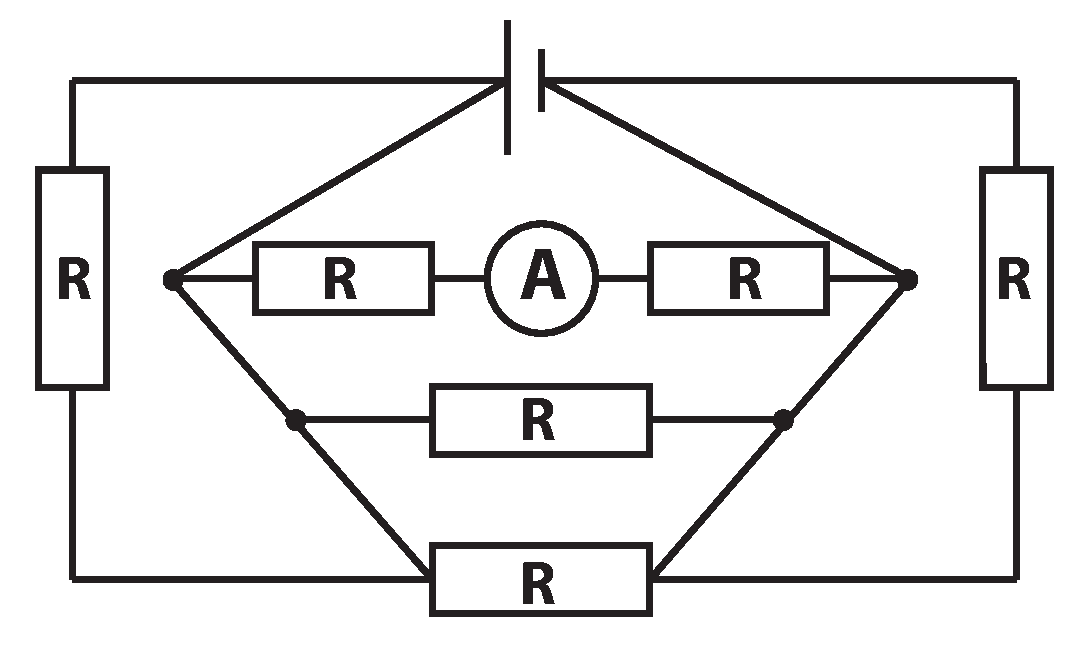
\includegraphics[width=0.4\textwidth]{2017-v2g-01-skeem}
\end{center}
\probend
\bigskip

% Ü52
\setAuthor{Mihkel Kree}
\setRound{piirkonnavoor}
\setYear{2015}
\setNumber{G 2}
\setDifficulty{2}
\setTopic{Elektriahelad}

\prob{Lambid}
Pingeallikaga on rööbiti ühendatud kaks lampi, kusjuures üks lampidest põleb $k$ korda suurema võimsusega kui teine. Seejärel ühendatakse need lambid sama pingeallikaga jadamisi. Mitu korda muutub lampidel eralduv koguvõimsus? Kas see muutub suuremaks või väiksemaks?
\pagebreak
\probend
\bigskip

% Ü53
\setAuthor{Oleg Košik}
\setRound{piirkonnavoor}
\setYear{2013}
\setNumber{G 5}
\setDifficulty{3}
\setTopic{Elektriahelad}

\prob{Elektriskeem}
\begin{wrapfigure}[7]{r}{2.5cm}%
\vspace{-12pt}
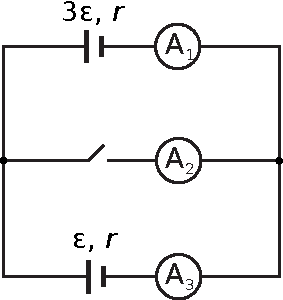
\includegraphics[width=\linewidth]{2013-v2g-05-skeem}%
\end{wrapfigure}
Joonisel toodud skeemil on ampermeetrid ideaalsed; patareide elektromotoorjõud
ja sisetakistused on märgitud nende juurde. Leidke ampermeetrite näidud, kui\\
\osa lüliti on suletud;\\
\osa lüliti on lahti.\\
\emph{Märkus}. praktikas tohib
sellist skeemi kasutada vaid siis, kui ollakse veendunud, et tekkivad voolud
jäävad ampermeetrite mõõtepiirkonda!
\probend
\bigskip

% Ü54
\setAuthor{Eero Vaher}
\setRound{lahtine}
\setYear{2014}
\setNumber{G 4}
\setDifficulty{3}
\setTopic{Elektriahelad}

\prob{Tetraeeder}
Tetraeedri (neljast võrdkülgsest kolmnurgast koosneva püramiidi) servadeks on ühesugused takistid takistusega $R$. Leidke tetraeedri kahe tipu vaheline takistus.
\probend
\bigskip

% Ü55
\setAuthor{Taavi Pungas}
\setRound{lõppvoor}
\setYear{2014}
\setNumber{G 1}
\setDifficulty{3}
\setTopic{Elektriahelad}

\prob{Ruudustik}
Traadist on valmistatud 2x2 ruudustik (vt joonist), iga väikese ruudu külje takistus on $r=\SI{1}{\ohm}$. Leidke punktide A ja B vaheline takistus.

\begin{center}
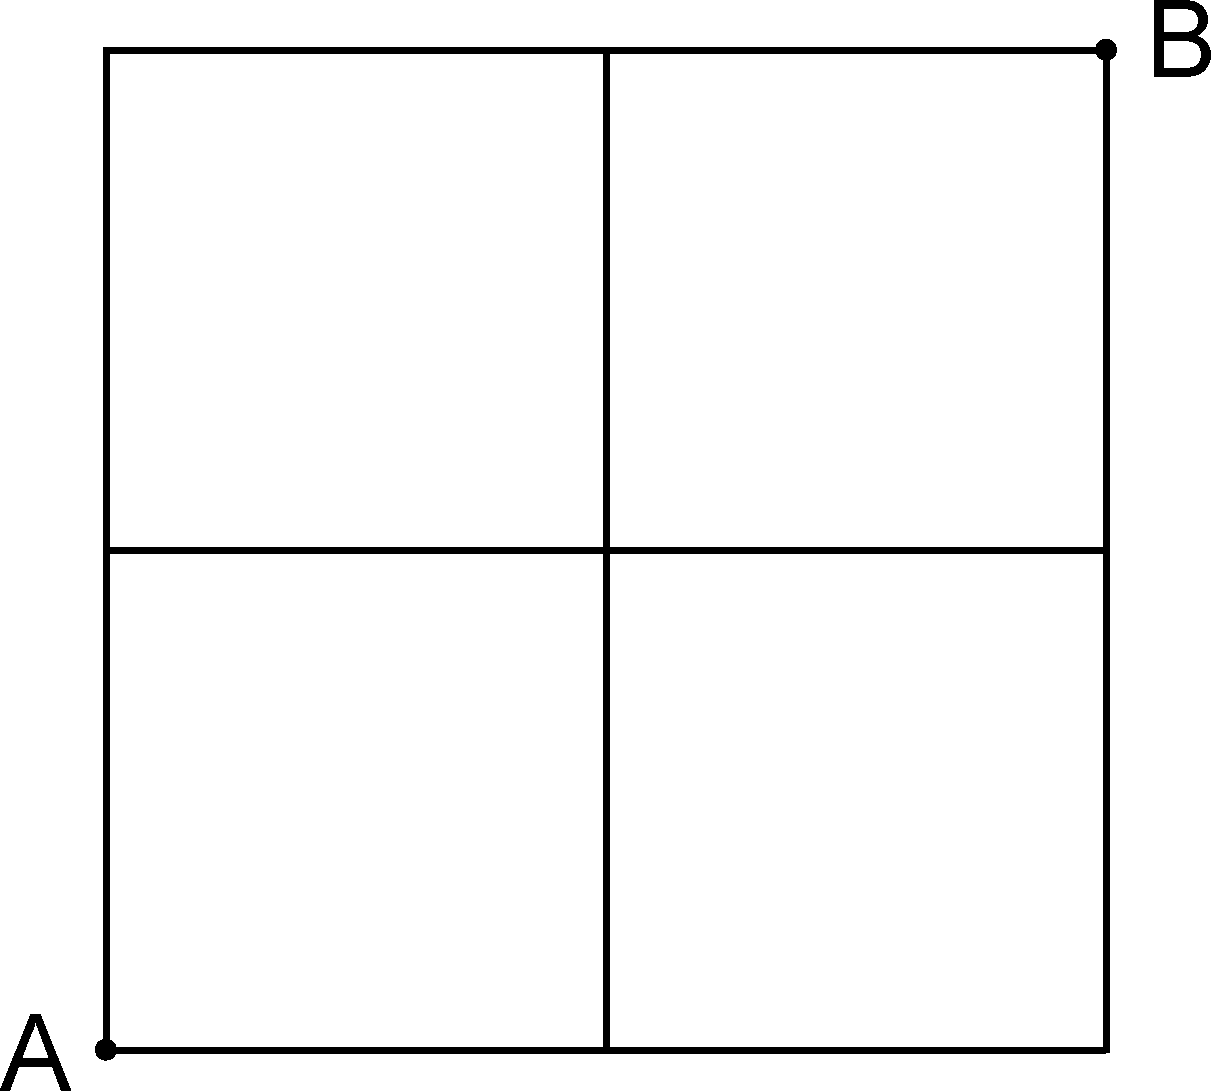
\includegraphics[width=0.2\linewidth]{2014-v3g-01-ruudustik}
\end{center}
\probend
\bigskip

% Ü56
\setAuthor{Hans Daniel Kaimre}
\setRound{lahtine}
\setYear{2015}
\setNumber{G 2}
\setDifficulty{3}
\setTopic{Elektriahelad}

\prob{Takistid}
Leidke ühesugustest takistitest koosneva ahela kogutakistus $R_{AB}$. Iga takisti takistus on $R$.

\begin{figure}[h]
\centering
\begin{circuitikz}[scale=0.9] \draw

(0,0) to [resistor] (0,2)
(0,0) to [resistor] (0,-2)
(0,0) to [resistor, *-*] (2,0)
(2,0) to [resistor] (4,0)
(4,0) to [resistor, *-*] (6,0)
(2,0) to [resistor, -*] (2,2)
(2,0) to [resistor, -*] (2,-2)
(4,0) to [resistor, -*] (4,2)
(4,0) to [resistor, -*] (4,-2)
(-1,0) to [short,o-] (0,0)
(6,0) to [short,-o] (7,0)
(0,2) -- (6,2) -- (6,0) -- (6,-2) -- (0,-2)
(-1,0) node[label={above:A}] {}
(7,0) node[label={above:B}] {}
;
\end{circuitikz}
\end{figure}
\probend
\bigskip

% Ü57
\setAuthor{Kristian Kuppart}
\setRound{lahtine}
\setYear{2016}
\setNumber{G 3}
\setDifficulty{3}
\setTopic{Elektriahelad}

\prob{Elektriskeem}
Leidke juuresoleval skeemil voolutugevus $I$ läbi ampermeetri kahel juhul: vahetult pärast lüliti sulgemist ja pika aja möödumisel. Eeldada, et kondensaatorid on enne lüliti sulgemist laadimata. Patarei lugeda ideaalseks.
\begin{center}
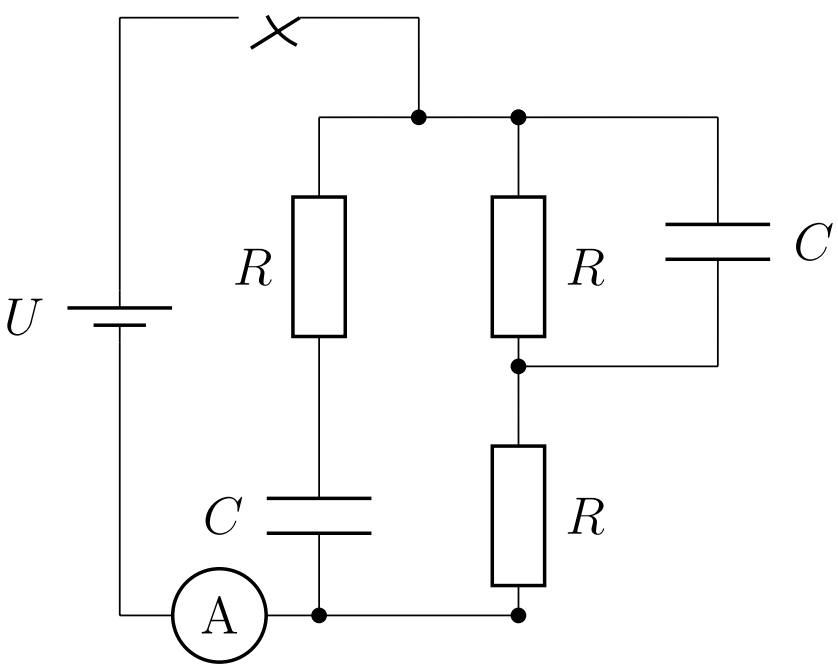
\includegraphics[width=0.45\textwidth]{2016-lahg-03-skeemjoonis.png}
\end{center}
\probend
\bigskip

% Ü58
\setAuthor{Kristian Kuppart}
\setRound{lõppvoor}
\setYear{2013}
\setNumber{G 4}
\setDifficulty{4}
\setTopic{Elektriahelad}

\prob{Must kast}
\begin{wrapfigure}{r}{0.35\textwidth}%
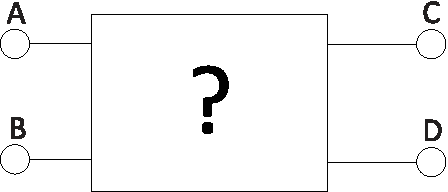
\includegraphics[width=\linewidth]{2013-v3g-04-pilt1}%
\end{wrapfigure}
Joonisel näidatud musta kasti kõik klemmid ühendatakse korraks kokku.
Seejärel, kui klemmide A ja B külge ühendada patarei
pingega $U$ ja klemmide C ja D külge voltmeeter, on voltmeetri näit alghetkel
$U$. Mõõtmise järel ühendatakse kõik klemmid veel korraks kokku.
Kui ühendada sama patarei klemmide C ja D külge ning voltmeeter
klemmide A ja B külge, on voltmeetri näit alghetkel~$\frac{U}{2}.$
Teades, et mustas kastis on ainult identsed kondensaatorid, joonistage musta kasti skeem.
\probend
\bigskip

% Ü59
\setAuthor{Sandra Schumann}
\setRound{lahtine}
\setYear{2017}
\setNumber{G 4}
\setDifficulty{4}
\setTopic{Elektriahelad}

\prob{Elektroonikaskeem}
\begin{wrapfigure}[5]{r}{0.57\textwidth}
	\vspace{-23pt}
	\begin{circuitikz} \draw
		(0.4,0.3) node {A}
		(-0.3,0.6) node {B}
		(-0.3,-0.6) node {C}
		(0,0) node[spdt, xscale=-1] (Sw) {}
		(Sw.out 1) -- (-1.5,0.31)
		(Sw.out 2) -- (-0.59, -1.5) -- (-1.5, -1.5)
		to[american voltage source, l=$9V$] (-1.5,0.31)
		(Sw.in) to[resistor, l=$R$] (3,0) -- (4,0) node[ocirc] {}
		(4.3,0) node {+}
		(4.3,-1.5) node {-}
		(4,-1.5) node[ocirc] {} -- (-0.59, -1.5)
		(3,-1.5) to[capacitor] (3,0)
		;
	\end{circuitikz}
\end{wrapfigure}

Joonisel on antud teatud elektroonikaseadme ühe osa skeem, mis koosneb \SI{9}{\volt} vooluallikast, takistist ja kondensaatorist koosnevast filtrist, väljundklemmidest ja lülitist. Lüliti kaks võimalikku asendit on \enquote{sees} (ühendatud on A ja B) ning \enquote{väljas} (ühendatud on A ja C). Antud olukorras ei ole väljundklemmide külge midagi ühendatud.

Kui toodud skeemis viia lüliti asendist \enquote{sees} asendisse \enquote{väljas} (st lülitada seade välja) ja muuta seejärel vooluallika polaarsus vastupidiseks, siis töötab elektroonikaseade pärast sisselülitamist endiselt. Kui aga vooluallika polaarsust muuta ilma seadet välja lülitamata, siis põleb takisti $R$ läbi. Eeldusel, et takisti põleb läbi niipea, kui sellel eralduv võimsus ületab \SI{0.25}{\watt}, leia $R$ minimaalne ja maksimaalne võimalik väärtus.
\probend
\bigskip

% Ü60
\setAuthor{Jaan Kalda}
\setRound{lõppvoor}
\setYear{2012}
\setNumber{G 3}
\setDifficulty{5}
\setTopic{Elektriahelad}

\prob{Elektriline sild}
Joonisel toodud skeemis on tegemist ühesuguste takistitega takistustega $R_1 = R_2 = R_3 = R_4 = R$ ning ühesuguste
ideaalsete patareidega elektromotoorjõududega ${\cal E}_1 = {\cal E}_2
= {\cal E}$. Leidke voolutugevused takistites (st $I_1$, $I_2$, $I_3$ ja
$I_4$ avaldised suuruste $R$ ja ${\cal E}$ kaudu).

\begin{center}
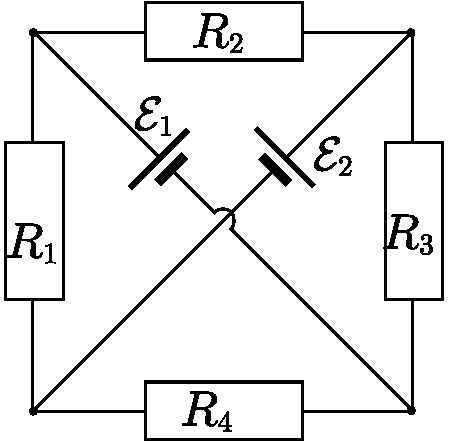
\includegraphics[width=0.35\linewidth]{2012-v3g-03-elektriline_sild}%
\end{center}
\probend
\bigskip

% Ü61
\setAuthor{Jaan Kalda}
\setRound{lõppvoor}
\setYear{2015}
\setNumber{G 4}
\setDifficulty{5}
\setTopic{Elektriahelad}

\prob{Must kast}
Mustas kastis on kolmest takistist ja ideaalsest ampermeetrist koosnev skeem. Lisaks on mustal kastil kolm väljundklemmi $A$, $B$ ja $C$. Kui rakendada pinge $U=\SI{12}{V}$ klemmide $A$ ja $B$ vahele, siis on ampermeetri näit $I_{AB}=\SI{2}{A}$. Klemmide $A$ ja $C$ puhul on lugem $I_{AC}=\SI{4}{A}$ ning klemmide $B$ ja $C$ puhul $I_{BC}=\SI{6}{A}$. Joonistage mustas kastis olev skeem ning märkige sellele takistite takistused.
\probend
\bigskip

% Ü62
\setAuthor{Jaan Kalda}
\setRound{lõppvoor}
\setYear{2017}
\setNumber{G 6}
\setDifficulty{5}
\setTopic{Elektriahelad}

\prob{Viisnurk}
Leidke joonisel toodud skeemis ampermeetri ja voltmeetri näidud. Kõik takistid on takistusega $R=\SI{1}{\ohm}$, pinge patarei klemmidel $U=\SI{7}{\volt}$.

\begin{center}
	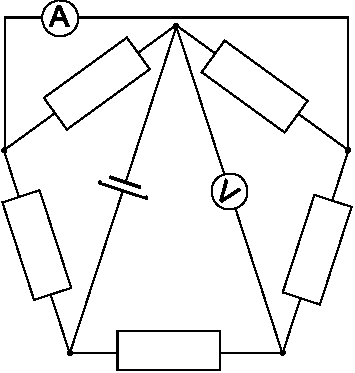
\includegraphics[width=0.4\textwidth]{2017-v3g-06-viisnurk}
\end{center}
\probend
\bigskip

% Ü63
\setAuthor{Valter Kiisk}
\setRound{piirkonnavoor}
\setYear{2018}
\setNumber{G 8}
\setDifficulty{5}
\setTopic{Elektriahelad}

\prob{12 lampi}
Juku käsutuses on 12 ühesugust taskulambipirni ning patarei, mille klemmipinge on täpselt 5 korda suurem pirni nimipingest. Lisaks leidis ta juhtumisi takisti, mille takistus on parajasti pool lambi hõõgniidi takistusest töörežiimis (viimase sai ta teada jagades lambi soklile kirjutatud nimipinge ja -voolu omavahel).\\
\osa Kuidas tuleb ühendada nimetatud komponendid elektriahelasse, et kõik 12 pirni põleksid normaalheledusega?\\
\osa Mitu korda kasvab (või kahaneb) lampide koguvõimsus, kui üks lampidest läbi põleb? Lampide takistuse sõltuvust temperatuurist võib jätta arvestamata.
\probend
\bigskip

% Ü64
\setAuthor{Eero Vaher}
\setRound{piirkonnavoor}
\setYear{2014}
\setNumber{G 8}
\setDifficulty{6}
\setTopic{Elektriahelad}

\prob{Elektriahela energia}
Suletud elektriahelas on jadamisi ühendatud takisti takistusega $R=\SI{100}{\ohm}$, kondensaator mahtuvusega $C=\SI{200}{\nano\farad}$, tühise aktiivtakistusega induktiivpool induktiivsusega $L=\SI{10}{\milli\henry}$ ning sobivalt ühendatud ideaalsed mõõteseadmed. Hetkel $t_0$ mõõdeti voolutugevuseks läbi kondensaatori $I=\SI{300}{\milli\ampere}$ ning pingeks poolil $U=\SI{50}{\volt}$. Teada on, et mõõtmise hetkel on vool poolis suunatud kõrgema potentsiaaliga piirkonnast madalama potentsiaaliga piirkonda. Kas mõõtmise hetkel $t_0$ oli rohkem energiat poolil või kondensaatoril?
\probend
\bigskip

% Ü65
\setAuthor{Sandra Schumann}
\setRound{lõppvoor}
\setYear{2016}
\setNumber{G 7}
\setDifficulty{6}
\setTopic{Elektriahelad}

\prob{Vooluallikad}
Vaatleme joonisel näidatud elektriskeemi, kus noolega tähistatud skeemielement on konstantse voolu allikas voolutugevusega $I=\SI{2}{mA}$ noolega tähistatud suunas. Leidke pinge $U$ väljundklemmidel ja voolutugevus läbi takisti $R=\SI{10}{k\ohm}$ kahe juhu jaoks: $\textbf{a)}$ kui lüliti K on suletud ja $\textbf{b)}$ kui lüliti on avatud.

\begin{center}
	\begin{circuitikz}[american voltages] \draw
		(0,0) to[battery1, l=\SI{1}{V}] (0,1.5)
		to[american current source, l=\SI{2}{mA}] (0,3) --(0,4)
		to[european resistor, l=\SI{10}{k\ohm}, *-] (2,4)
		to[battery1, l=\SI{2}{V}] (4,4)
		to[european resistor, l_=\SI{5}{k\ohm}, *-] (4,0) -- (5,0)
		to[battery1, l_=\SI{3}{V}] (5,4) -- (4,4)
		(4,0) to[short, *-*] (0,0)
		(0, 1.3) to[short,*-] (1.2, 1.3) -- (1.2, 2.05);\draw[thick] (1.2, 2.05) -- +(60:0.5) ;
		\draw (1.2,2.55) -- (1.2,3.3) to[short,-*] (0,3.3)
		(0,4) to[short, -*] (-2,4)
		to [open, v_<=$U$] (-2,0)
		to[short, *-] (0,0)
		
		(1.5, 2.2) node[right] {K};
	\end{circuitikz}
\end{center}
\probend
\newpage

\bigskip

% Ü66
\setAuthor{Eero Vaher}
\setRound{lõppvoor}
\setYear{2018}
\setNumber{G 7}
\setDifficulty{6}
\setTopic{Elektriahelad}

\prob{Takistuste tuvastamine}
\begin{wrapfigure}[10]{r}{0.4\textwidth}
\vspace{-20pt}
\begin{resizebox}{\linewidth}{!}{
\begin{circuitikz}
\draw
(1,0) to[battery1,l_=${U_0=\SI{14}{V},\,I_0=\SI{10}{A}}$] (8,0) to (1,0) to (1,2.5) to (2,2.5) to[short, *-] (2,4) to[resistor,l=${R_1}$, -*] (4.5,4) to[resistor,l=${R_4}$] (7,4) to[short, -*] (7,2.5) to (8,2.5) to (8,0)
(2,2.5) to (2,1) to[resistor,l=${R_2}$, -*] (4.5,1) to[resistor,l=${R_5}$] (7,1) to (7,2.5)
(4.5,1) to[resistor,l_=$R_3$] (4.5,4)
;
\draw[->,thick] (4,2) -- (4,3);
\end{circuitikz}}
\end{resizebox}
\end{wrapfigure}

Vooluallikaga on ühendatud viis takistit. Neist kolme takistus on \SI{1}{\ohm}, ülejäänud kaks on tundmatu, kuid ühesuguse takistusega. Vooluallika pinge $U_0=\SI{14}{V}$ ning voolutugevus selles $I_0=\SI{10}{A}$. Pinge ja voolutugevus kolmandal takistil on vastavalt $U_3=\SI{2}{V}$ ning $I_3=\SI{2}{A}$. Joonisel on märgitud elektrivoolu suund takistis $R_3$. Määrake kõigi takistite takistused.
\probend
\bigskip

% Ü67
\setAuthor{Mihkel Pajusalu}
\setRound{piirkonnavoor}
\setYear{2012}
\setNumber{G 8}
\setDifficulty{7}
\setTopic{Elektriahelad}

\prob{Raudtee}
\begin{wrapfigure}{r}{18mm}%
\vspace{-15pt}
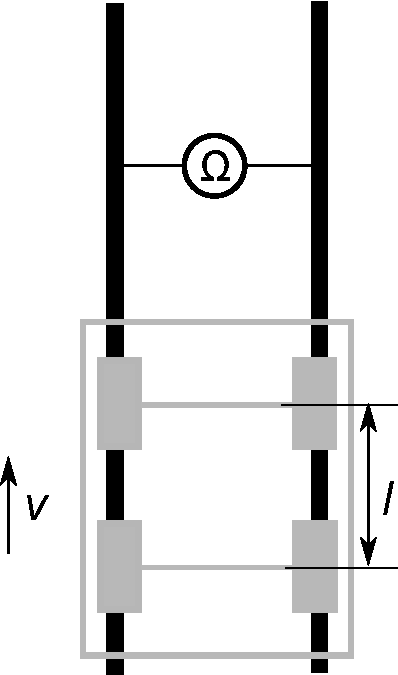
\includegraphics[width=\linewidth]{2012-v2g-08-rong}%
\end{wrapfigure}
Mõõdame raudteel elektritakistust kahe kõrvutise rööpa vahel nii, nagu joonisel.
Rööbastel sõidab vagun kiirusega $v$. Olgu vagunil kaks rattapaari,
mille vahekaugus on $l$. Joonistage graafik takistuse muutumisest ajas alates
hetkest, kui vaguni esimene rattapaar on mõõtepunkti ees sellest kaugusel $l/2$, kuni
ajani, kui tagumine rattapaar on mõõtepunkti taga sellest kaugusel $l/2$. Mõlema rattapaari
takistuseks olgu $r$ ja rööpa takistus pikkusühiku kohta $\rho$.
\probend
\bigskip

% Ü68
\setAuthor{Mihkel Kree}
\setRound{lahtine}
\setYear{2013}
\setNumber{G 9}
\setDifficulty{7}
\setTopic{Elektriahelad}

\prob{Lambid}
Juku ehitas kodus niisuguse elektriskeemi nagu joonisel näidatud, kasutades
selleks kuut ühesugust takistit takistusega $R=\SI{10}{\ohm}$, nelja
ühesugust lampi takistusega $r=\SI{20}{\ohm}$ ning pingeallikat
elektromotoorjõuga
$\mathcal{E}=\SI{5}{\volt}$. Arvutage igas lambis (joonisel tähised 1, 2, 3,
4) eralduv võimsus. Pingeallika sisetakistusega mitte arvestada.
\begin{center}
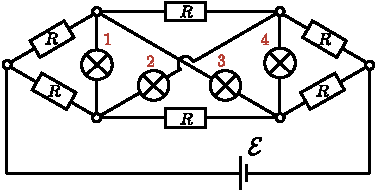
\includegraphics[width=0.6\linewidth]{2013-lahg-09-lambidJoonis-crop}
\end{center}
\probend
\newpage

\bigskip

% Ü69
\setAuthor{Jaan Kalda}
\setRound{lahtine}
\setYear{2012}
\setNumber{G 8}
\setDifficulty{8}
\setTopic{Elektriahelad}

\prob{Dioodid}
\begin{wrapfigure}{r}{0.4\linewidth}
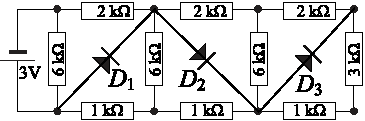
\includegraphics[width=\linewidth]{2012-lahg-08-dioodid}
\end{wrapfigure}
Millised võimsused eralduvad skeemil märgitud dioodidel? Dioodide voolu võib lugeda
nulliks kõikide vastupingete jaoks ning samuti ühest voldist
väiksemate päripingete jaoks; suvalise pärivoolu puhul on dioodi pinge
\SI{1,0}V. Takistite takistused ja elektromotoorjõu väärtus on toodud
joonisel. Dioodi skeemitähise noole suund näitab pärivoolu
suunda.
\probend
\bigskip

% Ü70
\setAuthor{Jaan Kalda}
\setRound{lahtine}
\setYear{2016}
\setNumber{G 8}
\setDifficulty{8}
\setTopic{Elektriahelad}

\prob{Oktaeeder}
Juuresolev skeem kujutab traadist oktaeedrit, iga traadi juurde on kirjutatud selle takistus oomides. 
Ampermeetreid ühendavad traadid on tühiselt väikese takistusega.
Leidke ampermeetrite näidud.

\begin{center}
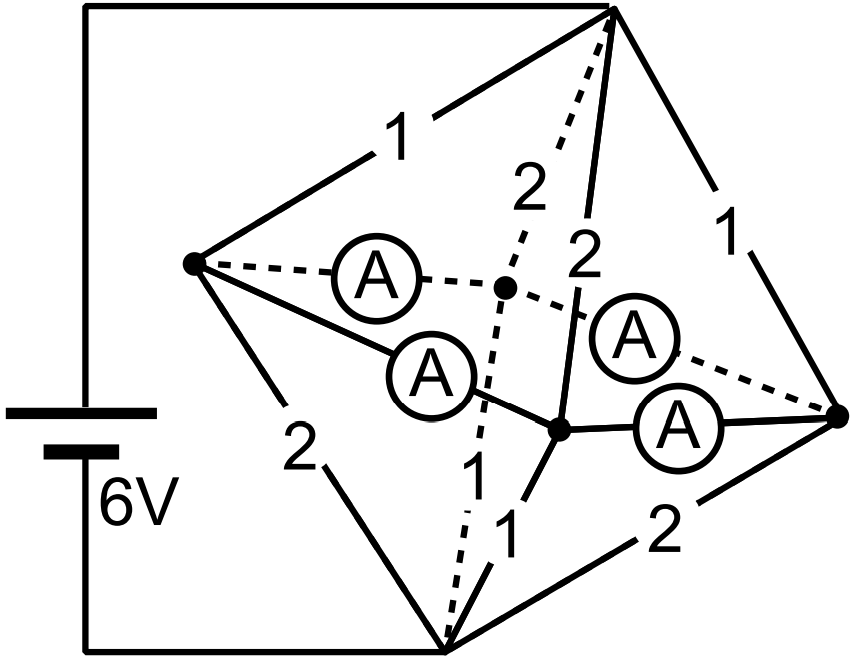
\includegraphics[width=0.5\textwidth]{2016-lahg-08-ampermeeterjoonis.png}
\end{center}
\probend
\bigskip

% Ü71
\setAuthor{Jaan Kalda}
\setRound{lõppvoor}
\setYear{2018}
\setNumber{G 9}
\setDifficulty{8}
\setTopic{Elektriahelad}

\prob{Kondensaator}
\begin{wrapfigure}[7]{r}{0.3\linewidth}
\vspace{-10pt}
\begin{center}
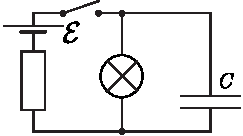
\includegraphics[width=\linewidth]{2018-v3g-09-LC-Q}
\par\end{center} 
\end{wrapfigure}

Vaatleme joonisel kujutatud elektriskeemi, mis koosneb kondensaatorist mahtuvusega $C$, patareist elektromotoorjõuga $\mathcal{E}$, takistist ja hõõglambist, mida võib lugeda mittelineaarseks takistiks (pinge sõltub voolust mittelineaarselt). Algselt oli kondensaator laenguta ja lüliti oli avatud. Seejärel suleti lüliti lühikeseks ajaks, misjärel see avati uuesti ning hoiti lahtisena seni, kuni kondensaator oli täielikult tühjenenud. Selle aja jooksul, mil lüliti oli suletud, eraldus kogu skeemil soojushulk $Q_1$; lüliti avamise järel eraldus täiendavalt veel soojushulk $Q_2$. Leidke laeng, mis läbis hõõglambi sel perioodil, kui lüliti oli suletud.
\probend
\newpage

\bigskip

% Ü72
\setAuthor{Jaan Toots}
\setRound{lõppvoor}
\setYear{2015}
\setNumber{G 10}
\setDifficulty{10}
\setTopic{Elektriahelad}

\prob{Türistor}
\begin{wrapfigure}{r}{0.48\textwidth}
\begin{circuitikz} \draw

(0,2) to[resistor=$R$] (2,2)
 to[Do,l=$T_1$, *-*] (2,0) -- (0,0)
 to[battery1,l=$U$] (0,2)
(2,2) to[switch] (4,2)
 to[Do,l=$T_2$] (4,0) -- (2,0)
;
\end{circuitikz}
\end{wrapfigure}
Türistori (dioodisarnase elemendi) volt-amper karakteristik on juuresoleval graafikul. Kaks sellist türistori on ühendatud pingeallika ja takistiga kõrvalolevasse skeemi. Takistus $R = \SI{2}{\kilo\ohm}$.\\
{\bf a}) Alguses on lüliti avatud. Pingeallika pinget suurendatakse lineaarselt $t=\SI{42}{\second}$ jooksul väärtuselt $U_0=\SI{0}{\volt}$ kuni väärtuseni $U_a = \SI{42}{\volt}$. Skitseerige ahelat läbiva voolutugevuse $I(t)$ sõltuvus ajast. Milline on voolutugevuse lõppväärtus $I_a$?\\
{\bf b}) Leidke lõppvoolutugevused mõlemas türistoris, kui lüliti suletakse ilma ahelale rakendatud pinget $U_a$ muutmata.

\begin{figure}[h]
\begin{center}
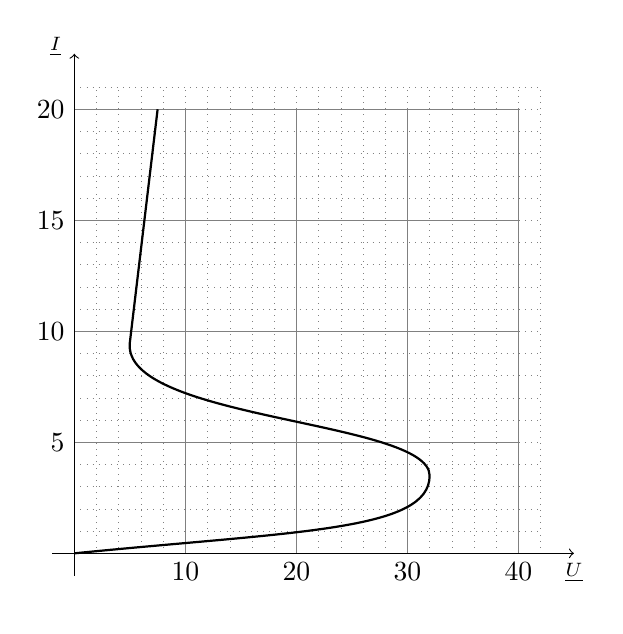
\begin{tikzpicture}[scale=1.41,
axes/.style=]

\draw[step=0.2, gray, dotted, very thin] (0,0) grid (4.2,4.2);
\draw[step=1, gray, very thin] (0,0) grid (4,4);

\begin{scope}[axes]
 \draw[->] (-0.2,0) -- (4.5,0) node[right, below] {$\frac{U}{\si{\volt}}$} coordinate(x axis);
 \draw[->] (0,-0.2) -- (0,4.5) node[above, left] {$\frac{I}{\si{\milli\ampere}}$} coordinate(y axis);

 \foreach \x/\xtext in {1/10, 2/20, 3/30, 4/40}
 \draw (\x,0) node[below] {$\xtext$};
 
 \foreach \y/\ytext in {1/5, 2/10, 3/15, 4/20}
 \draw (0,\y) node[left] {$\ytext$};
\end{scope}

\draw[thick] (0,0) .. controls (2,0.2) and (3.2,0.2) .. (3.2,0.7) .. controls (3.2,1.2) and (5/12,1.2) .. (0.5,1.9) -- (0.75,4);

\end{tikzpicture}

\end{center}
\end{figure}
\probend
\bigskip
\newpage\subsection{\protect\StrSubstitute{Elektrostaatika}{-}{ }}

% Ü73
\setAuthor{Madis Ollikainen}
\setRound{lahtine}
\setYear{2012}
\setNumber{G 3}
\setDifficulty{2}
\setTopic{Elektrostaatika}

\prob{Kondensaator}
Füüsikatudeng leidis vanade demonstratsioonideks mõeldud eksperimentaalseadmete
hulgast ühe plaatkondensaatori. Noore füüsikuna tundis ta kohe hirmsat soovi
sellega veidi mängida. Ta mõõtis kondensaatori plaatide vahekauguseks $d$
ning seejärel laadis kondensaatori pingeni $U$. Nüüd asetas ta
kondensaatori plaatide vahele ühe kuulikese, mis kukkus alumise plaadi peale
ja siis hakkas uuesti ülespoole tõusma. Kuulikesel kulus alumiselt plaadilt
ülemiseni jõudmiseks aeg $t$. Leidke kuulikese massi ja alumiselt plaadilt
saadud laengu suhe.
\probend
\bigskip

% Ü74
\setAuthor{Mihkel Kree}
\setRound{lahtine}
\setYear{2017}
\setNumber{G 3}
\setDifficulty{4}
\setTopic{Elektrostaatika}

\prob{Elektron}
\begin{wrapfigure}[7]{r}{0.5\linewidth}
	\vspace{-10pt}
	\hspace{-10pt}
	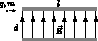
\includegraphics[width=\linewidth]{2017-lahg-03-elJoonisMK.pdf}
\end{wrapfigure}

Elektron liigub vaakumis ning siseneb paralleelsete plaatide vahel paiknevasse ruumipiirkonda selle ülemisest servast nii, et elektroni kiirusvektor on paralleelne plaatidega (vt joonist). Kui suur on elektroni minimaalne võimalik kiirus $v_\mathrm{min}$ plaatide vahelisest ruumipiirkonnast väljumisel? Plaatide pikkus on $l$ ja nende vahekaugus $d$. Plaatide vahel on ühtlane elektriväli $\vec{E}$ ning ääreefektidega pole vaja arvestada. Elektroni laeng on $q$ ning mass $m$. Gravitatsioonijõuga pole vaja arvestada.
\probend
\bigskip

% Ü75
\setAuthor{Mihkel Kree}
\setRound{piirkonnavoor}
\setYear{2017}
\setNumber{G 9}
\setDifficulty{6}
\setTopic{Elektrostaatika}

\prob{Laengud}
\begin{wrapfigure}{r}{0.3\textwidth}
	\vspace{-25pt}
	\begin{center}
		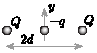
\includegraphics[width=0.32\textwidth]{2017-v2g-09-laengudjoonis.pdf}
	\end{center}
	\vspace{-10pt}
\end{wrapfigure}

Kaks kera, kumbki laenguga $Q$, on liikumatult fikseeritud nii, et nende keskpunktide kaugus on $2d$. Täpselt nende kerade keskele paigutatakse kolmas kera laenguga $-q$ ning massiga $m$, mis saab liikuda ainult mööda $y$-telge (vt joonis). Leidke selle kolmanda kera väikeste $y$-suunaliste võnkumiste periood $T$.
\probend
\bigskip

% Ü76
\setAuthor{Jonatan Kalmus}
\setRound{lõppvoor}
\setYear{2018}
\setNumber{G 6}
\setDifficulty{7}
\setTopic{Elektrostaatika}

\prob{Pendel}
Elektriliselt isoleeritud metallkuul massiga $M$ ja laenguga $Q>0$ ripub vertikaalse vedru otsas jäikusega $k$ tasakaaluasendis gravitatsiooniväljas $g$. Nüüd tekitatakse vertikaalne elektriväli tugevusega $E$, mis on esialgu suunatud alla ning edaspidi alati kuuli liikumise suunas. Eeldada, et elektriväli muutub hetkeliselt. Leida kuuli kaugus algsest asukohast ajahetkel $t=7\pi \sqrt{\frac{M}{k}}$.
\probend
\bigskip

% Ü77
\setAuthor{Stanislav Zavjalov}
\setRound{piirkonnavoor}
\setYear{2012}
\setNumber{G 10}
\setDifficulty{8}
\setTopic{Elektrostaatika}

\prob{Koonus}
Ühtlaselt laetud koonus kõrgusega $H$ tekitab oma tipus $S$ potentsiaali
$\varphi_0$. Sellest lõigatakse ära väiksem koonus kõrgusega $h$, mis on suure
koonusega sarnane, kahe koonuse tipud ühtivad. Seejärel eemaldatakse väiksem koonus
lõpmatusesse. Milline on uus potentsiaali väärtus punktis $S$?
\probend
\bigskip

% Ü78
\setAuthor{Jaan Kalda}
\setRound{lõppvoor}
\setYear{2012}
\setNumber{G 9}
\setDifficulty{8}
\setTopic{Elektrostaatika}

\prob{Laengud}
\begin{wrapfigure}{r}{0.33\textwidth}%
\vspace{-10pt}
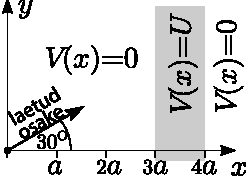
\includegraphics[width=\linewidth]{2012-v3g-09-laeng}%
\end{wrapfigure}
Positiivselt laetud osake kiirendatakse koordinaatide alguspunktis pinge $4U$ (kus $U>0$) abil teatud kiiruseni, mis
lebab $x-y$ tasandis $30$-kraadise nurga all $x$-telje suhtes, vt joonist. Elektriline potentsiaal $V(x,y)\equiv V(x)$
sõltub ainult $x$-koordinaadist: kui
$3a<x<4a$, siis $V(x)=U$ ning vastasel korral $V(x)=0$; peale elektrostaatilise jõu osakesele mingeid muid jõude ei mõju ning $a>0$.

\osa Visandage laengu trajektoor $x-y$-tasandis (geomeetrilisi mõõtmeid ja nurki pole vaja märkida).

\osa Nüüd on laetud osakeste allikaks koordinaatide alguspunktis asuv koaksiaalne vaakumdiood, mistõttu pinge $4U$
abil kiirendatud osakesi liigub isotroopselt (võrdsel hulgal) kõigis $x-y$-tasandi suundades;
$z$-suunaline kiiruskomponent on kõigil osakestel 0. Milline osa kõigist kiiratud osakestes jõuab ruumipiirkonda $x>4a$?
\probend
\bigskip

% Ü79
\setAuthor{Stanislav Zavjalov}
\setRound{lõppvoor}
\setYear{2013}
\setNumber{G 10}
\setDifficulty{8}
\setTopic{Elektrostaatika}

\prob{Kondensaator}
Ruudukujuliste plaatidega kondensaator plaadi pindalaga~$S$ ning plaatidevahelise
kaugusega $d \ll \sqrt{S}$ on laetud pingeni $U_0$ ning seejärel
patareist lahti ühendatud. Kondensaatori sisse viiakse ruudukujuline juhtiv
plaat, samuti pindalaga $S$ ning paksusega $d/2$, kuni plaat on täielikult
kondensaatori sees. Protsessi jooksul plaat ei puutu kokku
kondensaatori plaatidega ning on nendega paralleelne. Kui palju tööd tehti
plaadi sisseviimisel? Selgitage, kas plaat tõmbus ise sisse või pidid välisjõud
selle sisse lükkama. Servaefekte pole vaja arvesse võtta. Vaakumi dielektriline
läbitavus on $\varepsilon_0$.
\probend
\bigskip

% Ü80
\setAuthor{Jaan Kalda}
\setRound{lahtine}
\setYear{2017}
\setNumber{G 7}
\setDifficulty{8}
\setTopic{Elektrostaatika}

\prob{Kondensaator}
\begin{wrapfigure}[5]{r}{0.35\linewidth}
	\vspace{-13pt}
	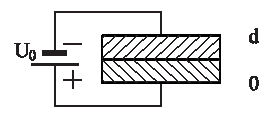
\includegraphics[width=\linewidth]{2017-lahg-07-res-cap2.pdf}
\end{wrapfigure}

Plaatkondensaator mahtuvusega $C$ omab plaatidevahelist kaugust $d$. Plaatide vahele asetatakse kaks dielektrilist plaati paksusega $d/2$. Ühe plaadi dielektriline läbitavus on $\varepsilon$, teisel $2\varepsilon$. Milline on nüüd kondensaatori mahtuvus? Milline laeng on plaatide eralduspinnal, kui kondensaatorile rakendatakse pinge $U_0$?
\probend
\bigskip

% Ü81
\setAuthor{Jaan Kalda}
\setRound{piirkonnavoor}
\setYear{2015}
\setNumber{G 10}
\setDifficulty{9}
\setTopic{Elektrostaatika}

\prob{Laengutega pulk}
\osa Dielektrikust pulk massiga $m$ ja pikkusega $L$ kannab kummaski otsas positiivset laengut $q$ (keskosa on laenguta, seega kogulaeng on $2q$). Piirkonnas $x<0$ on $x$-telje sihiline elektriväli tugevusega $E_0$ ja piirkonnas $x>0$ --- sama tugev $x$-teljega antiparalleelne elektriväli. Pulga keskpunt on koordinaatide alguspunktis ja pulk on paralleelne $x$-teljega. Pulgale antakse $x$-telje sihiline algkiirus $v$. Leidke võnkumiste periood. Pulk on paigaldatud nii, et see ei saa pöörelda, vaid üksnes liikuda $x$-telje sihis.

\osa Leidke väikeste võnkumiste periood siis, kui konfiguratsioon on muus osas sama, kuid punktlaengute asemel on kogulaeng $Q$ jaotunud ühtlaselt üle terve pulga.
\probend
\bigskip

% Ü82
\setAuthor{Jaan Kalda}
\setRound{lahtine}
\setYear{2016}
\setNumber{G 10}
\setDifficulty{9}
\setTopic{Elektrostaatika}

\prob{Kuulid}
Kaks metallkuulikest raadiusega $R$ on ühendatud peenikese metalltraadi abil ja asuvad homogeenses 
elektriväljas tugevusega $E$. Metalltraadi pikkus on $l$, kusjuures $l\gg R$. 
Süsteem on tasakaalus. Leidke mehaaniline pinge $T$ traadis.
\probend
\bigskip

% Ü83
\setAuthor{Jaan Kalda}
\setRound{lõppvoor}
\setYear{2018}
\setNumber{G 10}
\setDifficulty{9}
\setTopic{Elektrostaatika}

\prob{Kaks kuuli}
Kaks ühesugust metallkuuli raadiusega $R$ ja massiga $m$ on ühendatud peenikese terastraadiga pikkusega $L\gg R$. Piirkonnas $x\ge 0$ on elektriväli tugevusega $E$, mis on suunatud piki $x$-telge; piirkonnas $x< 0$ elektriväli puudub. Alghetkel on kuulid paigal ja üksteisest kaugusel $L$, nii et traat on pingul ning paralleelne $x$-teljega; ühe kuuli keskpunkt asub punktis $x=R$ ning teine kuul --- piirkonnas $x<0$. Visandage kvalitatiivselt kuulide kiiruse graafik sõltuvuses ajast (kvantitatiivset ajaskaalat ei ole vaja) ning leidke nende kiirus punkti $x=2L$ läbimisel. Terastraadi mahtuvus lugeda tühiselt väikeseks.
\probend
\bigskip

% Ü84
\setAuthor{Jaan Kalda}
\setRound{lõppvoor}
\setYear{2016}
\setNumber{G 10}
\setDifficulty{10}
\setTopic{Elektrostaatika}

\prob{Kolm kuuli}
Kolm väikest kuuli massiga $m$ kannavad ühesuguseid elektrilaenguid $q$ ning on ühendatud isoleerivast materjalist niitide abil võrdhaarseks kolmnurgaks $ABC$, kus $\angle BAC=120^\circ$ ning selle nurga tipus asuva kuuli $A$ vastaskülje niidi pikkus $|BC|=L$. Niit $BC$ lõigatakse katki. Leidke \osa kuuli $A$ maksimaalne kiirus edasise liikumise käigus ning \osa kuulikeste kiirendused vahetult pärast niidi läbi lõikamist. Gravitatsioonilise vastasmõjuga mitte arvestada.
\probend
\bigskip
\newpage\subsection{\protect\StrSubstitute{Gaasid}{-}{ }}

% Ü85
\setAuthor{Eero Vaher}
\setRound{lõppvoor}
\setYear{2015}
\setNumber{G 1}
\setDifficulty{2}
\setTopic{Gaasid}

\prob{Õhupall}
Heeliumiga täidetud õhupall suudab tõsta koormist massiga kuni $M=\SI{200}{kg}$. Kui suur on õhupalli ruumala $V$? Koormise ruumala lugeda tühiseks. Õhupalli kesta mass on arvestatud koormise massi sisse. Õhu tihedus on $\rho=\SI{1.2}{kg\per m^3}$, õhu rõhk $p=\SI{100}{kPa}$, õhu temperatuur $T=\SI{20}{\degreeCelsius}$. Heeliumi molaarmass on $\mu=\SI{4.0}{g\per mol}$, ideaalse gaasi konstant $R=\SI{8.3}{J\cdot mol^{-1}\cdot K^{-1}}$.
\probend
\bigskip

% Ü86
\setAuthor{Eero Vaher}
\setRound{lahtine}
\setYear{2013}
\setNumber{G 4}
\setDifficulty{3}
\setTopic{Gaasid}

\prob{Õhupalli vägi}
Heeliumiga täidetud õhupall suudab Maal tõsta õhku koormise massiga kuni
\SI{100}{\kilogram}. Kui suure massiga koormise suudaks samasugune õhupall
üles tõsta Marsil (õhupalli kesta massi loeme koormise massi hulka)? 
Koormise ruumala lugege tühiseks. Õhu tihedus Maal on
$\rho_0=\SI{1.2}{\kilogram\per\meter^3}$, õhu rõhk Maal
$p_0=\SI{100}{\kilo\pascal}$, õhu temperatuur Maal $T_0=\SI{20}{\degreeCelsius}$,
\enquote{õhu} tihedus Marsil $\rho_1=\SI{0.015}{\kilogram\per\meter^3}$, \enquote{õhu} rõhk Marsil
$p_1=\SI{600}{\pascal}$, \enquote{õhu} temperatuur Marsil $T_1=\SI{-60}{\degreeCelsius}$.
Heeliumi molaarmass on $\mu=\SI{4.0}{\gram\per\mole}$, ideaalse gaasi konstant
$R=\SI{8.3}{\joule\per\kelvin\per\mole}$.
\probend
\bigskip

% Ü87
\setAuthor{Mihkel Kree}
\setRound{lõppvoor}
\setYear{2014}
\setNumber{G 3}
\setDifficulty{4}
\setTopic{Gaasid}

\prob{Paisupaak}
Maja küttesüsteem sisaldab suurt akumulatsioonipaaki, kus hoitakse ringlevat sooja vett, ning paisupaaki, et kompenseerida vee soojuspaisumist. Paisupaak on fikseeritud ruumalaga anum, millest osa võtab enda alla õhk ning ülejäänu täidab küttesüsteemist pärinev vesi, mis saab vabalt süsteemi tagasi voolata. Hetkel, mil kogu vesi oli toatemperatuuril $t_0=\SI{20}{\degreeCelsius}$, täideti paisupaak suruõhuga nii, et õhu ruumala paagis oli $V_1=\SI{0.080}{m^3}$ ning rõhk $p_1=\SI{1.5}{}\,p_0$, kus $p_0=\SI{0.10}{\mega\pascal}$ on atmosfäärirõhk. Kogu süsteemis oleva vee ruumala toatemperatuuril on $V_0=\SI{1.0}{m^3}$.

Torustikus on ka avariiventiil, et vältida torude lõhkemist. Ventiil avaneb, kui rõhk torustikus ületab atmosfäärirõhku $\Delta p = \SI{1.2}{} \, p_0 $ võrra. Millise temperatuurini saab vett süsteemis soojendada, ilma et avariiventiil avaneks? Metalli soojuspaisumisega mitte arvestada. Vee tiheduse sõltuvus temperatuurist on toodud graafikul. Eeldage, et graafiku kuju ei sõltu rõhust (vaadeldavad rõhumuutused on selleks liiga väiksed). Samuti eeldage, et õhu temperatuur paisupaagis püsib toatemperatuuril $t_0$.

\begin{center}
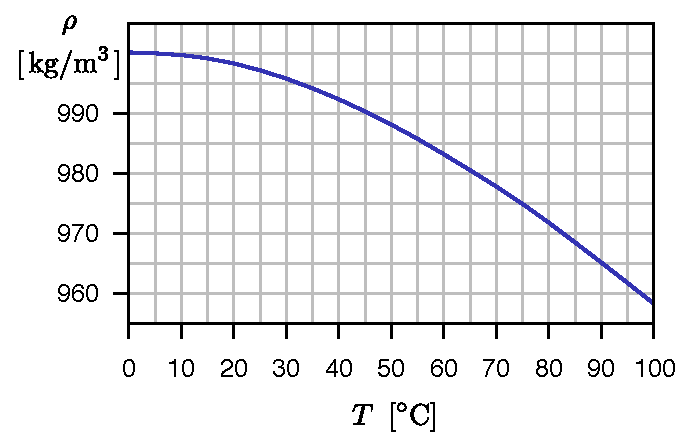
\includegraphics[width=0.8\linewidth]{2014-v3g-03-veeTihedus}
\end{center}
\probend
\bigskip

% Ü88
\setAuthor{Kaur Aare Saar}
\setRound{lahtine}
\setYear{2015}
\setNumber{G 3}
\setDifficulty{4}
\setTopic{Gaasid}

\prob{Balloon}
Pikk silindrikujuline balloon raadiusega $r=\SI{0,3}{m}$ on tehtud terasest, mis talub pindalaühiku kohta jõudu kuni $\sigma=\SI{250}{MPa}$. Leidke suurim balloonis oleva gaasi rõhk, mida balloon talub. Ballooni seina paksus on $t=\SI{2}{mm}$.
\probend
\bigskip

% Ü89
\setAuthor{Mihkel Kree}
\setRound{piirkonnavoor}
\setYear{2016}
\setNumber{G 5}
\setDifficulty{4}
\setTopic{Gaasid}

\prob{Saunauks}
Sauna leiliruumis ruumalaga $V=\SI{10}{m^3}$ on õhu temperatuur $t=\SI{90}{\degreeCelsius}$. Kerisele visatakse leiliks veekogus $m=\SI{150}{g}$, mis koheselt aurustub. Mõtleme hüpoteetiliselt, et leiliruum on hermeetiliselt suletud. Missuguse jõuga peaksid saunalised ust pindalaga $A=\SI{2,0}{m^2}$ käepidemest kinni hoidma, et see lahti ei läheks? Gaasikonstant $R=\SI{8.3}{J \per (mol\!\cdot\! K)}$ ning vee molaarmass $\mu=\SI{18}{g\per mol}$. Kui ülesande õigesti lahendate, siis küllap avastate, et leitud jõud on ebatavaliselt suur. Selgitage ühe lausega, miks tegelikult saunas ukse kinnihoidmiseks nii suurt jõudu pole vaja rakendada.
\probend
\bigskip

% Ü90
\setAuthor{Ardi Loot}
\setRound{lahtine}
\setYear{2017}
\setNumber{G 5}
\setDifficulty{4}
\setTopic{Gaasid}

\prob{Rattamatk}
Juku on rattamatkal ning soovib ratta tagumist rehvi natuke rohkem
täis pumbata. Et oleks lihtsam, kulutab Juku palju vaeva ja pakib
raske matkavarustuse pakiraamilt maha ja keerab ratta tagurpidi (rattad
taeva poole). Hinnake, mitu protsenti vähem jõudu peab ta pumpamisel
rakendama võrreldes olukorraga, kui tagumine ratas on koormatud?

\begin{wrapfigure}[5]{r}{0.4\linewidth}
	\vspace{-15pt}
	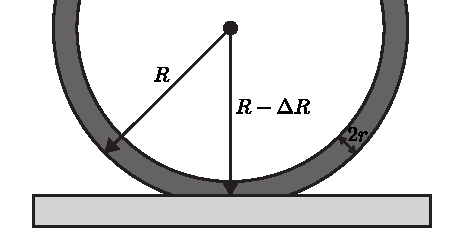
\includegraphics[width=\linewidth]{2017-lahg-05-fig_rattakumm.pdf}
\end{wrapfigure}

Ratta raadius $R=\SI{33.0}{cm},$ rehvi raadius $r=\SI{2.5}{cm},$
tagumisele rattale toetuv mass (ratas koos matkavarustusega) $m=\SI{30}{kg},$
koormatud rehvi rõhk $p=\SI{150}{kPa}$ (mõõdetud õhurõhu suhtes), õhurõhk $p_{0}=\SI{100}{kPa}$
ja raskuskiirendus $g=\SI{9.8}{m/s^{2}}.$ 

\textit{Vihje}. Koormamata rattarehvi ruumala on antud valemiga $V=2\pi^{2}\left(R-r\right)r^{2}$
ning see väheneb koormamisel $\Delta V\approx S\cdot\Delta R/2$ võrra,
kus $S\approx2\pi\Delta R\sqrt{Rr}$ on rehvi kokkupuutepinna suurus
maaga ja $\Delta R\ll r$ on rehvi deformatsiooni ulatus (vt joonist).
\probend
\bigskip

% Ü91
\setAuthor{Rasmus Kisel}
\setRound{piirkonnavoor}
\setYear{2017}
\setNumber{G 6}
\setDifficulty{4}
\setTopic{Gaasid}

\prob{Silinder külmkapis}
Suletud silindris sisemise raadiusega $R$ ja sisemise kõrgusega $h$ on vedelik, mis võtab enda alla teatud osa $k$ silindri siseruumalast. Silinder on algselt toatemperatuuril $T_{1}$. Silinder asetatakse sügavkülmikusse, kus on konstantne temperatuur $T_{2}$, mis on madalam silindris oleva aine sulamistemperatuurist. Teada on, et silindris oleva aine tihedus on vedelas olekus $\rho_0$ ja tahkes olekus $\lambda\rho_0$. Leidke, mitu korda suureneb silindris oleva õhu rõhk võrreldes esialgsega pärast vedeliku tahkumist. Eeldage, et vedeliku tahkumisel silindri mõõtmed ei muutu.
\probend
\bigskip

% Ü92
\setAuthor{Tundmatu autor}
\setRound{lahtine}
\setYear{2011}
\setNumber{G 5}
\setDifficulty{5}
\setTopic{Gaasid}

\prob{Süstal}
Kord sooritas noor füüsik eksperimendi, et leida süstlakolvile mõjuvat
hõõrdejõudu. Ta tõmbas $V_{0}=\SI{10}{ml}$ mahuga süstlasse \SI{5,0}{ml} õhku ja sulges siis
süstla otsa sõrmega. Seejärel tõmbas ta süstla kolvi näiduni
$V_{1}=\SI{9,2}{ml}$ ja
lasi sellel seejärel aeglaselt tagasi liikuda. Kolb liikus, kuni näiduks jäi $V_{2}=\SI{5,8}{ml}$.
Mõõtmisel selgus, et süstlakolvi sisediameeter oli $d=\SI{9}{mm}$ ja kraadiklaas
näitas, et ruumis oli $t=\SI{27}{\degreeCelsius}$, õhu suhteline niiskus $R=30\%$ ja õhurõhk
$p_{0}=\SI{103,6}{kPa}$. Milline oli süstlakolvile mõjuv hõõrdejõud?\\
\textit{Märkus.} Kuna tegu on praktilise probleemiga, siis ei pruugi kõik
algandmed vajalikud olla.
\probend
\bigskip

% Ü93
\setAuthor{Andreas Valdmann}
\setRound{piirkonnavoor}
\setYear{2012}
\setNumber{G 6}
\setDifficulty{5}
\setTopic{Gaasid}

\prob{Kuumaõhupall}
Mis temperatuurile tuleb kuumaõhupalli sees õhk kütta, et õhupall lendu tõuseks?
Välisõhu temperatuur $t=\SI{20}{\degreeCelsius}$, õhupalli ruumala $V=\SI{3000}{m^3}$ ja ei
muutu. Õhupalli kesta ja laadungi kogumass $m=\SI{700}{kg}$ ja õhu tihedus
20 kraadi juures $\rho_{20}=\SI{1,2}{kg/m^3}$.
\probend
\bigskip

% Ü94
\setAuthor{Andreas Valdmann}
\setRound{lõppvoor}
\setYear{2012}
\setNumber{G 4}
\setDifficulty{5}
\setTopic{Gaasid}

\prob{Korvpall}
NBA standarditele vastava korvpalli mass on $m=\SI{600}{g}$, ümbermõõt
$C=\SI{76}{cm}$ ning ülerõhk palli sees $p_1=\SI{55}{kPa}$. Kui sügavale vee
alla tuleks korvpall suruda, et see iseenesest põhja hakkaks vajuma? Vee tihedus
$\rho=\SI{1000}{kg/m^3}$, raskuskiirendus $g=\SI{9,8}{m/s^2}$ ja õhurõhk
veepinnal $p_0=\SI{100}{kPa}$. Võib eeldada, et sukeldamise jooksul palli sees
õhutemperatuur ei muutu ja palli kesta ruumala on tühine.
\probend
\bigskip

% Ü95
\setAuthor{Ardi Loot}
\setRound{lahtine}
\setYear{2016}
\setNumber{G 7}
\setDifficulty{6}
\setTopic{Gaasid}

\prob{Paisupaak}
Selleks, et vältida küttesüsteemis vee paisumise tulemusena tekkivat
ülerõhku, lisatakse süsteemi paisupaak. See koosneb silindrist ruumalaga
$V,$ mis on jaotatud vabalt liikuva õhukese vaheseinaga kaheks osaks. Üks
neist osadest täidetakse suruõhuga ($T_{0}=\SI{20}{\degreeCelsius}$)
rõhuni $p_{0}$, võttes enda alla kogu silindri ruumala. Seejärel ühendatakse silindri teine osa küttesüsteemiga temperatuuril $T_{1}=T_{0}$ ning süsteem täidetakse
veega, kuni saavutatakse rõhk $p_{1}=\SI{300}{kPa}$ ning vee koguruumala süsteemis $V_{s}=\SI{100}{L}$.
Täitmise lõppedes on paisupaagist $\beta=10\%$ täidetud veega. Talvel suureneb kütmise tõttu süsteemis oleva vee ruumala $\alpha=\SI{1}{\%}$ võrra, ning selle tulemusena tõuseb süsteemi rõhk $p_{2}$-ni, kusjuures paisupaagis olev õhk soojeneb temperatuurini $T_{2}=\SI{40}{\degreeCelsius}$. Leidke, kui suur peab olema paisupaagis
õhu algne rõhk $p_{0}$ ja minimaalne paisupaagi ruumala $V,$
et vee paisumise tulemusena tekkiv lisarõhk $\Delta p=p_{2}-p_{1}$
poleks suurem kui \SI{50}{kPa}.
\probend
\bigskip

% Ü96
\setAuthor{Valter Kiisk}
\setRound{piirkonnavoor}
\setYear{2017}
\setNumber{G 8}
\setDifficulty{7}
\setTopic{Gaasid}

\prob{Terasanum}
Sfäärilise terasanuma sisediameeter on $d=\SI{0.5}{m}$ ja mass $m=\SI{25}{kg}$. Maksimaalselt mitu liitrit gaasi (arvestatuna normaalrõhule) õnnestuks säilitada sellises anumas kõrge rõhu all? Terase tihedus on $\rho=\SI{7.9}{g/cm^3}$ ja maksimaalne talutav tõmbejõud pindalaühiku kohta $\sigma=\SI{450}{MN/m^2}$. Normaalrõhk on $p_0=\SI{101.3}{kPa}$.
\probend
\bigskip

% Ü97
\setAuthor{Ardi Loot}
\setRound{lõppvoor}
\setYear{2017}
\setNumber{G 7}
\setDifficulty{7}
\setTopic{Gaasid}

\prob{Õhupall}
Juku tahab õhupalli täis pumbata. Tal on suur pump, mille otsas olev ventiil on alguses suletud. Ta paneb pumba otsa õhupalli, seejärel vajutab pumbale peale, kuni rõhk pumbas tõuseb $p$-ni. Kokku surumise tõttu tõuseb pumbas oleva õhu temperatuur $T$-ni. Juku keerab ventiili lahti ja õhupall täitub aeglaselt, samal ajal vajub pumba käepide järjest allapoole. Juku vajutab kogu protsessi vältel pumbale täpselt sama suure jõuga kui alguses. Mis on õhu temperatuur õhupallis, kui see on täis pumbatud? Soojuskadudega läbi pumba ja õhupalli seinte mitte arvestada, samuti õhupalli kummi venitamisel tehtud tööga mitte arvestada. Väline õhurõhk ja temperatuur on $p_0$ ja $T_0$. Õhu soojumahtuvus konstantsel ruumalal on $c_V$.
\probend
\bigskip

% Ü98
\setAuthor{Ants Remm}
\setRound{piirkonnavoor}
\setYear{2014}
\setNumber{G 10}
\setDifficulty{8}
\setTopic{Gaasid}

\prob{Kuumaõhupall}
Juku läheb lendama kerakujulise kuumaõhupalliga, mille raadius $r = \SI{8.7}{\metre}$, mass koos reisijatega $M_0= \SI{390}{\kg}$ ning lisaks on kütusena kaasas $M_k = \SI{20}{\kg}$ propaani. Kui kaua saab kesta Juku õhupallilend? 

Õhupall on kaetud kattega, mis vähendab soojusjuhtivust ning soojuskiirgust tühiste väärtusteni. Tööolukorras imbub õhk läbi õhupalli kesta kiirusega $\lambda = \SI{500}{g\per\s}$. Õhurõhk ja temperatuur lennukõrgusel on $p_0 = \SI{100}{\kilo\Pa}$ ja $T_0 = \SI{10}{\degreeCelsius}$. Propaani kütteväärtus $k = \SI{50}{MJ/kg}$. Õhu keskmine molaarmass $\mu = \SI{29}{g\per\mole}$ ning soojusmahtuvus konstantsel rõhul $C_p = \SI{1.0}{\frac{kJ}{K\cdot kg}}$. Universaalne gaasikonstant on $R = \SI{8.3}{\frac{J}{K\cdot mol}}$.
\probend
\bigskip

% Ü99
\setAuthor{Jaan Kalda}
\setRound{lõppvoor}
\setYear{2018}
\setNumber{G 8}
\setDifficulty{8}
\setTopic{Gaasid}

\prob{Kerkiv õhupall}
Ilusa päikeselise ilma korral on harilikult tegemist nn adiabaatilise atmosfääriga. See tähendab, et õhumassid on pidevas üles-alla liikumises. Kerkides õhk paisub ja jahtub adiabaatiliselt; pideva segunemise tõttu on kerkiva õhumassi temperatuur võrdne seda antud kõrgusel ümbritsevate õhumasside temperatuuriga. On võimalik näidata, et sellisel juhul kahaneb temperatuur lineaarselt kõrgusega, $T=T_0-\frac{\gamma-1}\gamma\frac{\mu g h}R$, kus $\gamma=\SI{1.4}{	}$ on õhu adiabaadinäitaja, $\mu=\SI{29}{g/mol}$ --- õhu keskmine molaarmass, $g=\SI{9.81}{m/s^2}$ --- vabalangemise kiirendus, $R=\SI{8.31}{J/mol.K}$ --- gaasikonstant, ja $h$ --- kõrgus maapinnast; õhutemperatuur maapinnal $T_0=\SI{293}K$. Venimatust kuid vabalt painduvast nahast valmistatud õhupall mahutab maksimaalselt ruumala $V_0$ jagu gaasi; see täidetakse sellise koguse heeliumiga, mis võtab maapinnal enda alla ruumala $V_0/2$. Õhupall lastakse lahti ja see hakkab aeglaselt kerkima; lugeda, et õhupallis oleva heeliumi temperatuur on kogu aeg võrdne ümbritseva õhu temperatuuriga. Hinnake, millisel kõrgusel $h_1$ on õhupalli tõstejõud $1\%$ võrra väiksem kui maapinnal. Teilt oodatakse sellist hinnangut kõrgusele, mille suhteline viga pole suurem ühest kümnendikust, kusjuures vea piisavat väiksust pole vaja tõestada. 

\emph{Märkus.} Adiabaatilise protsessi korral kehtib seos $pV^\gamma = \const$, kus $p$ tähistab gaasi rõhku ja $V$ --- ruumala.
\probend
\bigskip
\newpage\subsection{\protect\StrSubstitute{Geomeetriline optika}{-}{ }}

% Ü100
\setAuthor{Roland Matt}
\setRound{lahtine}
\setYear{2011}
\setNumber{G 1}
\setDifficulty{2}
\setTopic{Geomeetriline optika}

\prob{Segadus optikalaboris}
Optik koristas vana laborit ja leidis sealt ühe markeerimata nõgusläätse ja ühe
kumerläätse. Nende optiliste tugevuste määramamiseks paigutas ta läätsed
üksteise taha ja lasi neist läbi kaks paralleelset laserkiirt, mille vahekaugus
oli $x_{1}=\SI{1,0}{cm}$. Ta muutis läätsede vahekaugust seni, kui süsteemist väljunud
kiired olid jällegi paralleelsed (seda kontrollis ta, määrates nende vahekaugust
paberilehekesega erinevatel kaugustel), nüüd oli kiirte vahekauguseks
$x_{2}=\SI{26}{mm}$. Sellises olukorras oli läätsedevaheliseks kauguseks 
$d=\SI{32}{cm}$.
Millise optilise tugevusega olid läätsed?
\probend
\bigskip

% Ü101
\setAuthor{Koit Timpmann}
\setRound{piirkonnavoor}
\setYear{2016}
\setNumber{G 3}
\setDifficulty{2}
\setTopic{Geomeetriline optika}

\prob{Lääts}
Punkt $A$ ja selle tõeline kujutis $A'$ asuvad läätse optilisest peateljest vastavalt \SI{4}{cm} ja \SI{1}{cm} kaugusel. Punktist $A$ kuni selle kujutiseni $A'$ on otsejoones \SI{15}{cm}. Kui suur on läätse fookuskaugus?
\probend
\bigskip

% Ü102
\setAuthor{EFO žürii}
\setRound{lahtine}
\setYear{2017}
\setNumber{G 2}
\setDifficulty{2}
\setTopic{Geomeetriline optika}

\prob{Valgusallika kujutis}
Sama suure fookuskauguse absoluutväärtusega $f$ kumer- ja nõguslääts asuvad nii, et nende fookused ning optilised peateljed ühtivad. Läätsede ees optilisel peateljel kumerläätsest kaugusel $\num{1,5}f$ asub punktvalgusallikas $A$. Leidke punktvalgusallika kujutise asukoht läbi kahe läätse. Tehke joonis.
\probend
\bigskip

% Ü103
\setAuthor{Aigar Vaigu}
\setRound{piirkonnavoor}
\setYear{2017}
\setNumber{G 4}
\setDifficulty{2}
\setTopic{Geomeetriline optika}

\prob{Piiritusetehas}
Piiritusetehases mõõdetakse piirituse ja vee segus oleva piirituse mahuprotsenti joonisel näidatud optilise seadme abil, kus segu paikneb kanalis laiusega $d=\SI{1}{cm}$. 
Kui suure vahemaa võrra muutub seadme fototundlikul elemendil kiire asukoht, kui piiritus mahuprotsendiga \SI{40}{\percent} asendada piiritusega mahuprotsendiga \SI{85}{\percent}?
Võib eeldada, et segu murdumisnäitaja $n\idx{segu}$ on lineaarne kombinatsioon vee ja piirituse murdumisnäitajatest
$$
n\idx{segu}=Xn\idx{piiritus}+(1-X)n\idx{vesi},
$$
kus X on piirituse mahuline sisaldus vahemikus 0 -- 1 ja $n\idx{piiritus}=\num{1,3615}$ ning $n\idx{vesi}=\num{1,3330}$.

\begin{center}
	\vspace{-0pt}
	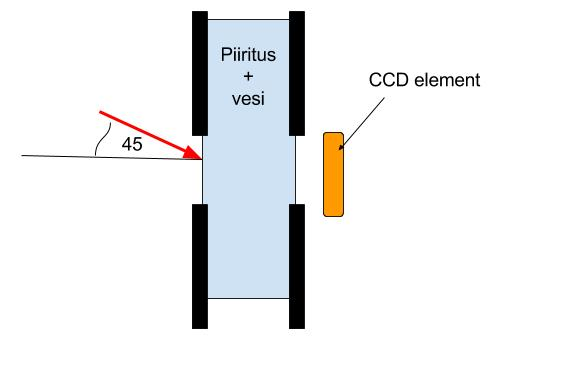
\includegraphics[width=0.5\linewidth]{2017-v2g-04-Piiritusetehas.jpg}
	\vspace{-10pt}
\end{center}
\probend
\bigskip

% Ü104
\setAuthor{EFO žürii}
\setRound{piirkonnavoor}
\setYear{2018}
\setNumber{G 2}
\setDifficulty{2}
\setTopic{Geomeetriline optika}

\prob{Kaks valgusallikat}
Kaks punktikujulist valgusallikat asuvad kumerläätse optilisel peateljel erinevates punktides. Nendest valgusallikatest läätse abil tekitatud kujutised kattuvad. On teada, et üks valgusallikas asub läätse keskpunktist $a=\SI{18}{cm}$ kaugusel. Kui kaugel sellest valgusallikast asub teine valgusallikas? Läätse fookuskaugus $f=\SI{9}{cm}$.
\probend
\bigskip

% Ü105
\setAuthor{Hans Daniel Kaimre}
\setRound{lõppvoor}
\setYear{2018}
\setNumber{G 1}
\setDifficulty{2}
\setTopic{Geomeetriline optika}

\prob{Poolitatud lääts}
Kersti paneb kokku optilise skeemi, nii et koondav lääts on objektist ja ekraanist, kuhu terav kujutis tekib, võrdsel kaugusel. Ta jätab objekti ja ekraani asukoha samaks, kuid lõikab läätse optilise peatelje juurest pooleks ning nihutab kaks tekkinud poolikut läätse optilisest peateljest eemale. Joonistage lisalehel uue skeemi jaoks kiirte käik. Objekt on tähistatud A-ga.
\begin{center}
 \begin{tikzpicture}[scale=0.5]

 % Def. koordinaadid
 \coordinate (O) at (0,0) ;
 \coordinate (A) at (-8,0) ;
 \coordinate (A') at (8,0) ;
 \coordinate (1) at (0,2);
 \coordinate (2) at (0,6);
 \coordinate (3) at (0,-2);
 \coordinate (4) at (0,-6);
 \coordinate (K) at (-6,4);
 \coordinate (KO) at (-6,0);
 

 % Jooned, t2pid
 \draw[thick] (A) -- (A');
 \draw[thick][->] (1) -- (2);
 \draw[thick][->] (3) -- (4);
 \pgfsetarrowsstart{latex}
 \draw[ultra thick] (K) -- (KO) ;
	
 % Nurgad ja punktid
 \node[] at (-7.0,4) {A};
 
\end{tikzpicture}
\end{center}
\probend
\bigskip

% Ü106
\setAuthor{Taavi Pungas}
\setRound{lahtine}
\setYear{2012}
\setNumber{G 4}
\setDifficulty{3}
\setTopic{Geomeetriline optika}

\prob{Kärbes}
Kumerläätse optilisel peateljel, kaugusel $a$ läätsest, lendab kärbes.
Kärbse kiirus on $v$ ning tema suund on risti optilise peateljega.
Leidke kärbse kujutise kiirus (nii suund kui väärtus). Läätse
fookuskaugus on $f < a$.
\probend
\newpage

\bigskip

% Ü107
\setAuthor{Oleg Košik}
\setRound{piirkonnavoor}
\setYear{2012}
\setNumber{G 1}
\setDifficulty{3}
\setTopic{Geomeetriline optika}

\prob{Peegel}
Suure ruumi seinal on \SI{2,0}{m} laiune peegel. Peegli kõrval \SI{2,0}{m}
kaugusel peeglist ja \SI{1,0}{m} kaugusel seinast seisab inimene, kes hakkab
liikuma paralleelselt peegliga kiirusega \SI{1,0}{m/s}. Samal hetkel hakkab
minema mööda peegli keskjoont peegli poole kiirusega \SI{1,0}{m/s} tema tuttav,
kes alghetkel seisab \SI{3,5}{m} kaugusel peeglist. Millise aja pärast
märkavad tuttavad teineteist peeglis?

\begin{center}
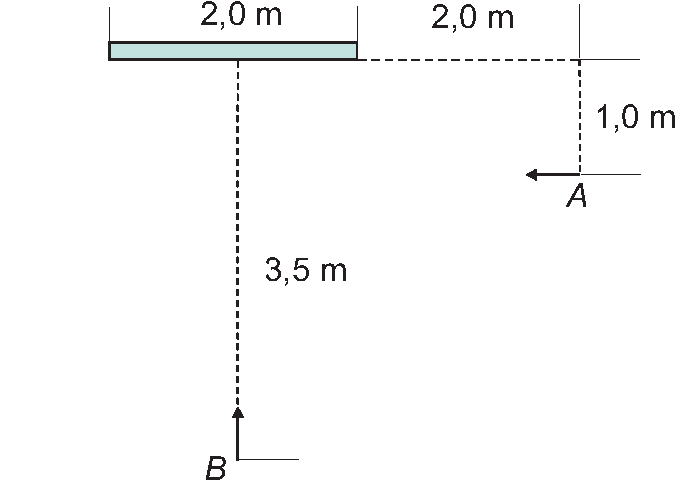
\includegraphics[width=0.5\linewidth]{2012-v2g-01-peegel2}%
\end{center}
\probend
\bigskip

% Ü108
\setAuthor{Tanel Kiis}
\setRound{lõppvoor}
\setYear{2013}
\setNumber{G 1}
\setDifficulty{3}
\setTopic{Geomeetriline optika}

\prob{Läätsed}
Jukul on suur hulk nõgusläätsi, mille fookuskauguste leidmiseks ta konstrueeris lihtsa
süsteemi. Ta suunas optilise peateljega paralleelse
laserikiire läbimõõduga $2R$ tuntud fookuskaugusega
$f_1$ koondava läätse keskpunkti, pärast mida koondus laserkiir ekraanil ühte punkti. Kui nüüd panna
fookuskaugusega $f_2$ nõguslääts võrdsele kaugusele koondavast läätsest ja
ekraanist, on laserkiire läbimõõt ekraanil~$2r$. Leidke $f_2$ eeldusel, et~$2f_2 < f_1$.
\probend
\bigskip

% Ü109
\setAuthor{Valter Kiisk}
\setRound{lõppvoor}
\setYear{2015}
\setNumber{G 2}
\setDifficulty{3}
\setTopic{Geomeetriline optika}

\prob{Valgustamine}
Lääts fookuskaugusega $f_1=\SI{4}{cm}$ on paigutatud nii, et läätsele suunatud paralleelsete valguskiirte kimp diameetriga $d_0=\SI{1}{cm}$ koondub ekraanil ühte punkti. Mõnikord on tarvis valgustada ekraanil suuremat ala, kuid läätse nihutamine või valgusallika vahetamine pole võimalik. Kui suur peab olema olemasolevast läätsest paremale paigutatava lisaläätse fookuskaugus $f_2$, et ekraanil tekiks ühtlaselt valgustatud laik diameetriga $d=\SI{2}{cm}$, kui läätsede vahekaugus on $L$?
\begin{center}
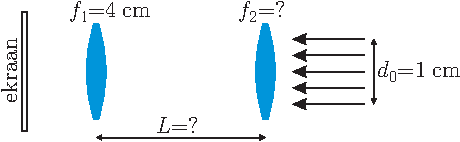
\includegraphics[scale=1.5]{2015-v3g-02-valgustamine-yles}
\end{center}
\probend
\bigskip

% Ü110
\setAuthor{Andreas Valdmann}
\setRound{lahtine}
\setYear{2016}
\setNumber{G 4}
\setDifficulty{4}
\setTopic{Geomeetriline optika}

\prob{Optiline kiud}
Optiline kiud koosneb silindrikujulisest klaassüdamikust murdumisnäitajaga $n_1=\SI{1,46}{}$ ja seda toruna ümbritsevast kattest murdumisnäitajaga $n_2=\SI{1,44}{}$. Leidke pikast optilisest kiust väljuva valguskoonuse tipunurk, lähtudes klassikalisest optikast.
\probend
\bigskip

% Ü111
\setAuthor{Andres Põldaru}
\setRound{lahtine}
\setYear{2016}
\setNumber{G 5}
\setDifficulty{4}
\setTopic{Geomeetriline optika}

\prob{Kolmlääts}
\begin{wrapfigure}[8]{r}{0.6\textwidth}
	\vspace{-20pt}
	\begin{resizebox}{0.6\textwidth}{!}{
\begin{tikzpicture}
\draw[{Stealth[scale=1.0]}-{Stealth[scale=1.0]}, line width=1pt] (0,0)-- ++(30:5);
\draw[{Stealth[scale=1.0]}-{Stealth[scale=1.0]}, line width=1pt] (30:5)-- ++(-90:5);%
\draw[{Stealth[scale=1.0]}-{Stealth[scale=1.0]}, line width=1pt] (0,0)-- ++(-30:5);
%\draw[->] (0,0) -- (5,0);
\node at (5.77,0) {\textbullet} (5.77,0) node[anchor=west] {$B$};
\node at (-2.89,0) {\textbullet} (-2.89,0) node[anchor=east] {$A$};
\draw[decorate,decoration={brace,raise=2pt,amplitude=6pt}] (0,0) -- node[below right = 7pt and -10pt]{$2f$} (-2.89,0) ;
\draw[decorate,decoration={brace,raise=2pt,amplitude=6pt}] (5.77,0) -- node[below right = 7pt and -8pt]{$f$} (4.33,0) ;
\end{tikzpicture}}
	\end{resizebox}
\end{wrapfigure}

Kolm läätse on kokku pandud nii, et nendest tekib võrdkülgne kolmnurk. Läätsedel on üks ühine fookus. Punktvalgusallikas pannakse punkti A, mis on kolmnurga tipust kaugusel $2f$, kus $f$ on läätsede fookuskaugus. Põhjendada konstrueerimise teel, kas osa valgusest jõuab punkti B.
\probend
\bigskip

% Ü112
\setAuthor{Eero Vaher}
\setRound{piirkonnavoor}
\setYear{2017}
\setNumber{G 5}
\setDifficulty{4}
\setTopic{Geomeetriline optika}

\prob{Puuduv lääts}
Esemelt lähtuv valgus läbib esmalt nõgusläätse ning seejärel kumerläätse. Joonisel on kujutatud eseme, kumerläätse ning lõpuks tekkiva kujutise asukohad ning kumerläätse fookused $F_k$. Konstrueerige lisalehel nõgusläätse ning selle esemepoolse fookuse $F_n$ asukohad. 

\begin{resizebox}{\linewidth}{!}{
		\begin{tikzpicture}
		\pgfmathsetmacro{\fk}{2}
		\pgfmathsetmacro{\tk}{3*\fk}
		\pgfmathsetmacro{\nk}{1/(1/\fk-1/\tk)}
		\pgfmathsetmacro{\a}{2*\fk}
		\pgfmathsetmacro{\h}{0.5}
		\pgfmathsetmacro{\htk}{\tk/\nk*\h}
		\pgfmathsetmacro{\ha}{1.5*\h}
		\pgfmathsetmacro{\nl}{\nk-\h/(\h-\ha)*(\nk-\a)}
		\pgfmathsetmacro{\fn}{\nk-\h/(\h-\ha)*(\nk-\nl)}
		\coordinate (TK) at (\tk, -\htk);
		\coordinate (NK) at (-\nk, \h);
		\coordinate (A) at (-\a, \ha);
		\draw (-1.1*\fn, 0) -- (1.1*\tk, 0);
		\draw[<->, ultra thick] (0,3.5*\h) -- (0,-3.5*\h);
		\draw[->, ultra thick] (\tk, 0) -- (TK);
		\draw[fill] (-\fk, 0) circle (0.02*\fk) node[below] {$F_k$};
		\draw[fill] (\fk, 0) circle (0.02*\fk) node[below] {$F_k$};
		\draw[->, ultra thick] (-\a, 0) -- (A);
		\end{tikzpicture}}
\end{resizebox}
\probend
\bigskip

% Ü113
\setAuthor{Andreas Valdmann}
\setRound{lõppvoor}
\setYear{2014}
\setNumber{G 4}
\setDifficulty{5}
\setTopic{Geomeetriline optika}

\prob{Periskoopprillid}
\begin{wrapfigure}{r}{0.38\textwidth}
 \begin{center}
 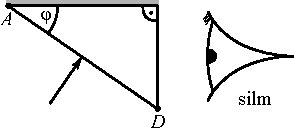
\includegraphics[width=0.4\textwidth]{2014-v3g-04-periskoopprillid_yl_joonis.pdf}
 \end{center}
\end{wrapfigure}

Kui liiga kaua järjest raamatut lugeda, võib kael pikast allapoole vaatamisest ära väsida. Selle vältimiseks on välja mõeldud erilised prillid, mille abil saab pead kallutamata alla vaadata. Prillide põhiliseks elemendiks on joonisel kujutatud prisma, mille pealmine tahk on kaetud valgust peegeldava materjaliga. Prisma tipunurk $\varphi$ on valitud selliselt, et kui prismasse sisenev valguskiir on pinnaga risti, siis on seda ka väljuv kiir. Prisma on tehtud materjalist murdumisnäitajaga $n=\SI{1,5}{}$. 

\osa Lõigul $AD$ on punktid $B$ ja $C$, mis jagavad selle kolmeks piirkonnaks: $AB$, $BC$ ning $CD$. Sõltuvalt sellest, millisele piirkonnale kiir langeb, on kiire käiguks prismas kolm põhimõtteliselt erinevat võimalust. Tehke joonis kiirte käigust kõigi juhtude jaoks.\\
\osa Leidke nurga $\varphi$ väärtus.\\
\osa Olgu külje $AD$ pikkus $l$. Kui kaugel asuvad punktid $B$ ja $C$ tipust $A$?\\
\osa Miks on prillides üldsegi vaja kasutada suhteliselt keerulist prismaga süsteemi, selle asemel et kiirte kallutamiseks kasutada ühte tasapeeglit?
\probend
\bigskip

% Ü114
\setAuthor{Mihkel Kree}
\setRound{lahtine}
\setYear{2015}
\setNumber{G 5}
\setDifficulty{5}
\setTopic{Geomeetriline optika}

\prob{Lääts}
Joonisel on kujutatud objekt AB ning sellest kumerläätses tekkinud tõeline kujutis A'B'. Leidke konstrueerimise teel läätse keskpunkti ning fookuse asukoht.

\begin{center}
 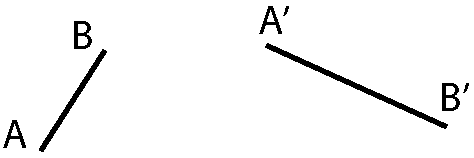
\includegraphics[width=0.7\linewidth]{2015-lahg-05-laatsMihkel.pdf}
\end{center}
\probend
\bigskip

% Ü115
\setAuthor{Sandra Schumann}
\setRound{lõppvoor}
\setYear{2018}
\setNumber{G 3}
\setDifficulty{5}
\setTopic{Geomeetriline optika}

\prob{Peegelpõhi}
Peegelpõhjaga tühja anumasse paigutatakse koondav klaaslääts nii, et läätse optiline peatelg on risti anuma põhjaga. Läätse kaugus anuma põhjast on $l=\SI{10}{cm}$. Läätsele suunatakse paralleelne valgusvihk, mis koondub pärast läätse läbimist mingis punktis $A$. Siis valatakse anum vett täis (lääts jääb vee alla). Valgusvihk koondub endiselt samas punktis $A$. Leidke läätse fookuskaugus $f$ õhus.

Klaasi murdumisnäitaja $n_k = \SI{1,49}{}$, vee murdumisnäitaja $n_v = \SI{1,33}{}$, õhu oma $n_0 = \SI{1,0}{}$. Murdumisnäitaja näitab, kui mitu korda on valguse kiirus vaakumis suurem kui aines.

\emph{Märkus.} Läätse fookuskauguse $f_v$ leidmiseks vees kehtib valem 
%\[ \frac {f_1}{f_2} = \frac{n_{lääts} n_1 - n_1 n_2}{n_{lääts} n_2 - n_1 n_2} \]
\[ f_v = f\cdot\frac{n_k n_v - n_0 n_v}{n_k n_0 - n_0 n_v}. \]
%kus $f_0$ on läätse fookuskaugus õhus, $f_v$ vees. $n_o$ õhu murdumisnäitaja, $n_v$ vee murdumisnäitaja ja $n_k$ läätse materjali murdumisnäitaja.
\probend
\newpage

\bigskip

% Ü116
\setAuthor{Eero Vaher}
\setRound{piirkonnavoor}
\setYear{2015}
\setNumber{G 8}
\setDifficulty{6}
\setTopic{Geomeetriline optika}

\prob{Fookuskaugus}
Õhukese tasanõgusa läätse parem külg on hõbetatud. Kui suur on sellise optilise elemendi fookuskaugus $f$ vasakult langeva valguse jaoks? Läätse nõgusa osa kõverusraadius on $R$, läätse materjali murdumisnäitaja ümbritseva keskkonna suhtes on $n$.

\begin{center}
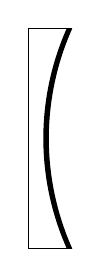
\begin{tikzpicture}[scale=0.7, transform shape]
\def\tmp{65.92}
\fill [black] (0.7,2) arc[start angle=90+\tmp, end angle=270-\tmp,radius=4.9] -- (0.8,-2) -- (0.8,-2) arc[start angle=270-\tmp, end angle=90+\tmp,radius=4.9] -- (0.7,2);
\draw (0.8,-2) -- (0,-2) -- (0,2) -- (0.8,2);
\end{tikzpicture}
\end{center}
\probend
\bigskip

% Ü117
\setAuthor{Jaan Kalda}
\setRound{lõppvoor}
\setYear{2012}
\setNumber{G 6}
\setDifficulty{7}
\setTopic{Geomeetriline optika}

\prob{Toru}
Peegeldavate siseseintega toru põhjas on punktvalgusallikas, vt joonist. Toru
sisediameeter on
$d=\SI{12}{mm}$, toru pikkus $l=\SI{60}{mm}$. Vastu toru lahtist otsa on
paigutatud koondav lääts fookuskaugusega $F=\SI{36}{mm}$ ning toru otsast
kaugusele $L=\SI{90}{mm}$ ekraan, millele kinnitatud millimeeterpaberile
on märgitud lõikepunkt optilise peateljega $O$.
Visandage kujutis, mida võib näha ekraanil.

\begin{center}
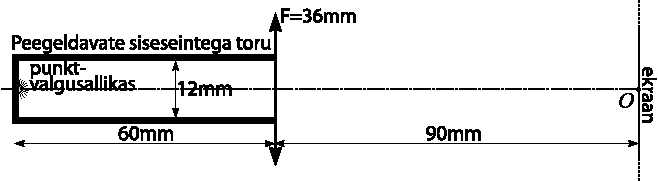
\includegraphics[width=\textwidth]{2012-v3g-06-toru-valgusallikas-lxxts}
\end{center}
\probend
\bigskip

% Ü118
\setAuthor{Valter Kiisk}
\setRound{lõppvoor}
\setYear{2013}
\setNumber{G 7}
\setDifficulty{7}
\setTopic{Geomeetriline optika}

\prob{Mikroskoop}
Nn digitaalne mikroskoop koosneb piki optilist peatelge nihutatavast
läätsest (objektiivist), mis tekitab vaadeldavast esemest tõelise kujutise
elektroonilise maatrikssensori pinnale. Terav kujutis tekib objektiivi kahe
erineva asendi korral. Vastavate joonsuurenduste suhteks määrati 25. Kummas
asendis ja mitu korda on sensori pinnaühikule langev kiirgusvõimsus suurem?
Võib eeldada, et läätse mõõtmed on palju väiksemad tema kaugusest objektist.
\probend
\newpage
\bigskip

% Ü119
\setAuthor{Erkki Tempel}
\setRound{lahtine}
\setYear{2014}
\setNumber{G 7}
\setDifficulty{7}
\setTopic{Geomeetriline optika}

\prob{Optiline skeem}
\begin{wrapfigure}{r}{0.5\textwidth}
 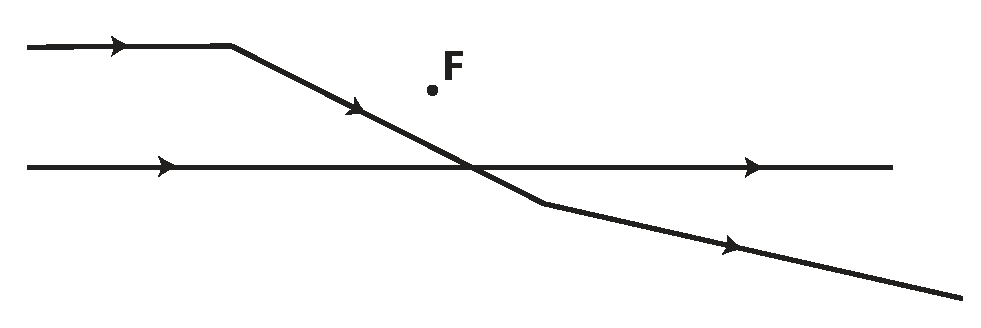
\includegraphics[width=0.5\textwidth]{2014-lahg-07-optilineskeemjoonis}
\end{wrapfigure}
Kõrvaloleval joonisel on kujutatud kahe algselt paralleelse kiire käik läbi kahe ühesuguse kumerläätse, mis ei asetse paralleelselt. Läätsede fookused ühtivad ning asuvad punktis F. Konstrueerige skeemile läätsed koos optiliste peatelgedega.
\probend
\bigskip

% Ü120
\setAuthor{Valter Kiisk}
\setRound{lõppvoor}
\setYear{2016}
\setNumber{G 6}
\setDifficulty{7}
\setTopic{Geomeetriline optika}

\prob{Luup}
Kui asetada poolkera-kujuline klaaskeha (lääts) tasapinnalise poolega vastu paberit, on võimalik vähemalt läätse keskosa ümbruses näha paberi pinna suurendatud kujutist. Kui mitmekordne kujutis saadakse, vaadeldes kauguselt, mis on hulga suurem läätse mõõtmetest? Klaasi murdumisnäitaja $n=\num{1.5}$.
\probend
\bigskip

% Ü121
\setAuthor{Andreas Valdmann}
\setRound{lõppvoor}
\setYear{2016}
\setNumber{G 8}
\setDifficulty{8}
\setTopic{Geomeetriline optika}

\prob{Nurgapeegel}
\begin{wrapfigure}{r}{0.35\textwidth}
	\vspace{-25pt}
	\begin{center}
		
\includegraphics[width=0.35\textwidth]{2016-v3g-08-wink.png}
	\end{center}
	\vspace{-20pt}
\end{wrapfigure}

Jukul oli katsetamiseks kolm ruudukujulist tasapeeglit. Ühte peeglisse vaadates ja paremat silma kinni pigistades nägi ta endast joonisel kujutatud peegelpilti. Järgmisena paigutas Juku kolm peeglit sedasi, et need moodustasid kuubi kolm tahku, millel on üks ühine tipp. Sealjuures jäid peegelpinnad kuubi sisemisele poolele. Joonistage peegelpilt, mida paremat silma kinni pigistav Juku endast otse nurgapeegli nurka vaadates nägi ja põhjendage tulemust konstrueerimise teel.
\probend
\bigskip

% Ü122
\setAuthor{Jaan Kalda}
\setRound{lõppvoor}
\setYear{2015}
\setNumber{G 7}
\setDifficulty{9}
\setTopic{Geomeetriline optika}

\prob{Ring ja ellips}
Juuresoleval joonisel on kujutatud ring ja sellest koondava läätse poolt tekitatud kujutis. Leidke läätse keskpunkt, optiline peatelg ja fookus.
\begin{center}
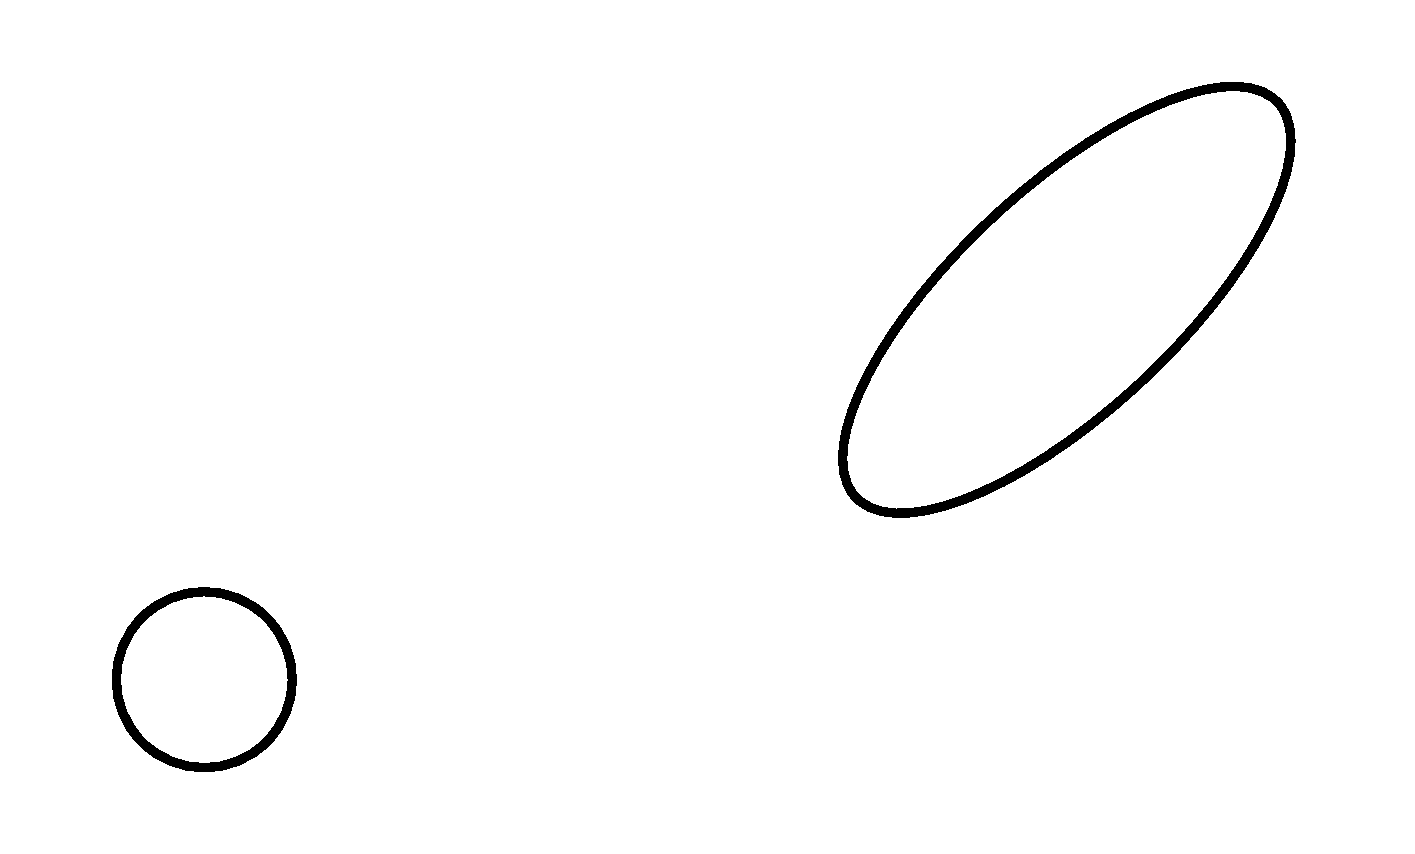
\includegraphics[width=0.7\textwidth]{2015-v3g-07-ringjaellips}%
\end{center}
\probend
\bigskip

% Ü123
\setAuthor{Ardi Loot}
\setRound{lõppvoor}
\setYear{2017}
\setNumber{G 8}
\setDifficulty{9}
\setTopic{Geomeetriline optika}

\prob{Kaamera}
Juku pildistab virmalisi iseehitatud kaameraga, mis koosneb ruudukujulisest
valgustundlikust elemendist küljepikkusega $2h=\SI{2.0}{cm}$ ja kumerläätsest
fookuskaugusega $f=\SI{14}{cm}.$ Jukule ei meeldi, et kaamera on
niivõrd suur ja ta tahab, et kaamera oleks maksimaalselt $L_{m}=\SI{7.0}{cm}$
pikk (kaamera pikkus on kaugus valgustundlikust elemendist välimise läätseni).
Selleks paigaldab ta vana kumerläätse asemel uue kumerläätse fookuskaugusega $f_{2}=\SI{3.0}{cm}$
valgustundlikust elemendist kaugusele $L_{m}.$ Kui suure fookuskaugusega
ja kui kaugele kumerläätsest peaks Juku süsteemi
lisama ühe nõgusläätse, et säiliks kaamera esialgne vaatenurk?
\probend
\bigskip

% Ü124
\setAuthor{Jaan Kalda}
\setRound{lõppvoor}
\setYear{2014}
\setNumber{G 10}
\setDifficulty{10}
\setTopic{Geomeetriline optika}

\prob{Klaassilinder}
Klaassilindri välispinnal märgitakse markeriga punkt. Kui seda silindrit vaadata suurelt kauguselt (hulga suuremalt kui silindri raadius) nii, et punkt paistab läbi silindri selle sümmeetriateljel olevat, siis on lisaks näha veel kahte punkti kujutist. Üks kujutis on näha ühel ja teine teisel pool sümmeetriatelge. Kui silindrit keerata ümber oma sümmeetriatelje, siis teatud hetkel sulavad kaks punkti kujutist kokku ning kaovad ära. Kolmas kujutis jääb alles. Kui silindrit edasi keerata, siis hetkel, kui selle pöördenurk algasendi suhtes on \ang{15}, kaob ka kolmas kujutis, nõnda et markeriga tehtud punkti polegi enam näha. Kui suur on klaasi murdumisnäitaja?
\probend
\bigskip
\newpage\subsection{\protect\StrSubstitute{Kinemaatika}{-}{ }}

% Ü125
\setAuthor{Koit Timpmann}
\setRound{piirkonnavoor}
\setYear{2013}
\setNumber{G 1}
\setDifficulty{1}
\setTopic{Kinemaatika}

\prob{Rong}
Kaubarong läbis kahe jaama vahelise teelõigu keskmise kiirusega \SI{36}{km/h}.
Kogu sõiduajast 2/5 vältel liikus rong ühtlaselt kiirenevalt, siis 2/5 vältel
liikus jääva kiirusega ning viimase 1/5 vältel pidurdas ühtlaselt aeglustuvalt.
Kui suur oli rongi maksimaalne kiirus kahe jaama vahelisel teel?
\probend
\bigskip

% Ü126
\setAuthor{Mihkel Kree}
\setRound{lahtine}
\setYear{2015}
\setNumber{G 1}
\setDifficulty{2}
\setTopic{Kinemaatika}

\prob{Rongivile}
Rong läheneb jaamale sirgjooneliselt ning muutumatu kiirusega. Vedurijuht laseb vilet kestusega $t_0=\SI{10}{s}$, peatuses rongi ootav jaamaülem mõõdab vile kestuseks aga $t_1=\SI{9}{s}$. Arvutage rongi liikumise kiirus $v$. Heli kiirus õhus $c=\SI{340}{m/s}$.
\probend
\bigskip

% Ü127
\setAuthor{Erkki Tempel}
\setRound{piirkonnavoor}
\setYear{2015}
\setNumber{G 1}
\setDifficulty{2}
\setTopic{Kinemaatika}

\prob{Kaubarong}
Tavaliselt sõidab kaubarong ühtlase kiirusega $v=\SI{72}{km/h}$, kuid seekord hilines jaama $\Delta t=\SI{5}{min}$. Raudteel olid hooldetööd ning rong pidi mingi aja sõitma kiirusega $v_{h}=\SI{18}{km/h}$. Rongi kiirendus pidurdamisel oli $a_p=\SI{0,2}{m/s^2}$ ning kiirendamisel $a_k=\SI{0,1}{m/s^2}$. Kui pika tee sõitis rong kiirusega \SI{18}{km/h}?
\probend
\bigskip

% Ü128
\setAuthor{Sandra Schumann}
\setRound{lahtine}
\setYear{2017}
\setNumber{G 1}
\setDifficulty{2}
\setTopic{Kinemaatika}

\prob{Kiirabiauto}
Jukust sõitis tänaval mööda kiirabiauto. Juku kuulis, et möödumisel langes kiirabiauto sireeni toon väikese tertsi võrra. Kui kiiresti sõitis kiirabiauto? Heli kiirus õhus Juku juures oli $v_h = \SI{343}{\meter\per\second}$. Eeldada, et Juku kaugus kiirabiauto sirgjoonelisest trajektoorist on tühiselt väike. Doppleri seadus annab seose sageduste ja liikumiskiiruste vahel.
\[ \frac{f_v}{f_a} = \frac{v_h + v_v}{v_h + v_a} \ , \]
kus \(f_v\) on vastuvõtja mõõdetud heli sagedus, \(f_a\) on allika tekitatud heli sagedus, \(v_v\) on heli vastuvõtja kiirus ja \(v_a\) on heliallika liikumise kiirus.

\emph{Vihje}. Väike terts on muusikaline intervall, mis vastab \num{1.5}-toonisele erinevusele heli sageduses. Üks oktav tähistab 2-kordset erinevust heli sageduses ja vastab 6 toonile. Eeldada, et toonid on jaotatud oktavis nõnda, et kui kolme helisageduse $f_1, f_2, f_3$ jaoks kehtib $\frac{f_2}{f_1} = \frac{f_3}{f_2}$ ja $f_1$ ning $f_2$ vahel on üks toon, siis on ka $f_2$ ja $f_3$ vahel üks toon.
\probend
\bigskip

% Ü129
\setAuthor{Mihkel Rähn}
\setRound{piirkonnavoor}
\setYear{2017}
\setNumber{G 2}
\setDifficulty{2}
\setTopic{Kinemaatika}

\prob{Pidurdus}
Kaks autot sõidavad teineteise järel kiirustega $v=\SI{50}{km/h}$. Esimene auto pidurdab maksimaalselt, mida nähes tagumise auto juht samuti pidurdab maksimaalselt. Esimese auto pidurid rakenduvad samal hetkel, kui süttivad pidurituled. Tagumise auto juhil kulub eesmise auto piduritulede süttimisest kuni oma auto pidurite rakendumiseni $t=\SI{1,5}{s}$. Teekatte hõõrdetegur $\mu=1$ ning raskuskiirendus $g=\SI{9,8}{m/s^2}$.\\
\osa Kui suur peaks olema autodevaheline vahemaa sõidu ajal, et pidurdamisel ei toimuks tagant otsasõitu?\\
\osa Kui autodevaheline vahemaa enne pidurdamist on $l=\SI{5}{m}$, siis kui suur on autode kiirus üksteise suhtes kokkupõrke hetkel?
\probend
\bigskip

% Ü130
\setAuthor{Jaan Kalda}
\setRound{lõppvoor}
\setYear{2013}
\setNumber{G 3}
\setDifficulty{4}
\setTopic{Kinemaatika}

\prob{Jalgrattur}
Poiss mõõdab jalgrattaga sõites tuule kiirust enda suhtes: kui ta sõidab piki teed ühes
suunas kiirusega \SI{10}{km/h}, saab ta tulemuseks \SI{20}{km/h}, ning kui ta sõidab
vastassuunas kiirusega \SI{20}{km/h}, siis saab ta tulemuseks samuti
\SI{20}{km/h}. Kui kiiresti maa suhtes puhub tuul?
\probend
\bigskip

% Ü131
\setAuthor{Jaan Toots}
\setRound{lõppvoor}
\setYear{2014}
\setNumber{G 2}
\setDifficulty{4}
\setTopic{Kinemaatika}

\prob{Viiul}
Viiulikeelt pikkusega $L$ kaugusel $\frac{3}{7}L$ ühest otsast alla vajutades ning lühemal osal poognaga tõmmates kõlab mingi põhisagedusega heli. Samal kaugusel $\frac{3}{7}L$ keelt ainult puudutades (alla vajutamata), on kõlav heli erinev. Milline on nende kahe põhisageduse suhe?
\probend
\bigskip

% Ü132
\setAuthor{Taavi Pungas}
\setRound{piirkonnavoor}
\setYear{2012}
\setNumber{G 4}
\setDifficulty{5}
\setTopic{Kinemaatika}

\prob{Pöördlava}
Sageli on teatrilava põranda osaks pöörlev ketas. Näitleja soovib sellise ketta
kõrval olevast punktist $A$ ajaga $t$ jõuda võimalikult kaugele mõnda teise ketta
kõrval olevasse punkti. Kus asub selline kaugeim sihtpunkt $B$? Väljendage vastus nurgana
$\alpha = \angle \mathit{AOB}$, kus $O$ on ketta keskpunkt. Näitleja kõnnib
kiirusega $v$, ketta pöörlemisperiood on $T$ ja raadius $r$. Võite eeldada, et $\alpha < \ang{180}$.
\probend
\bigskip

% Ü133
\setAuthor{Eero Vaher}
\setRound{lõppvoor}
\setYear{2015}
\setNumber{G 5}
\setDifficulty{5}
\setTopic{Kinemaatika}

\prob{Pallivise}
Juku elab silindrikujulises kosmosejaamas, mille pöörlemine tekitab kunstliku raskusjõu. Jaama raadius on $R$, selle pöörlemise nurkkiirus $\omega$. Juku viskab palli otse üles algkiirusega $v=\frac{\sqrt{3}}{3}\omega R$. Kui kaugele Jukust mööda jaama pinda pall maandub?
\probend
\bigskip

% Ü134
\setAuthor{Siim Ainsaar}
\setRound{lõppvoor}
\setYear{2012}
\setNumber{G 5}
\setDifficulty{6}
\setTopic{Kinemaatika}

\prob{Rehvid}
Et autorehvid kuluksid vähimal määral, tasub auto ehitada nii, et kurvis
pöörduksid esirattad eri nurga võrra. Leidke selles mõttes parim parema
esiratta pöördenurk $\beta$ paremkurvis, kus
vasaku esiratta oma on $\alpha$. Rataste vahekaugus on pikkupidi $a$ ja laiupidi
$b$ (vt joonist).
\begin{center}
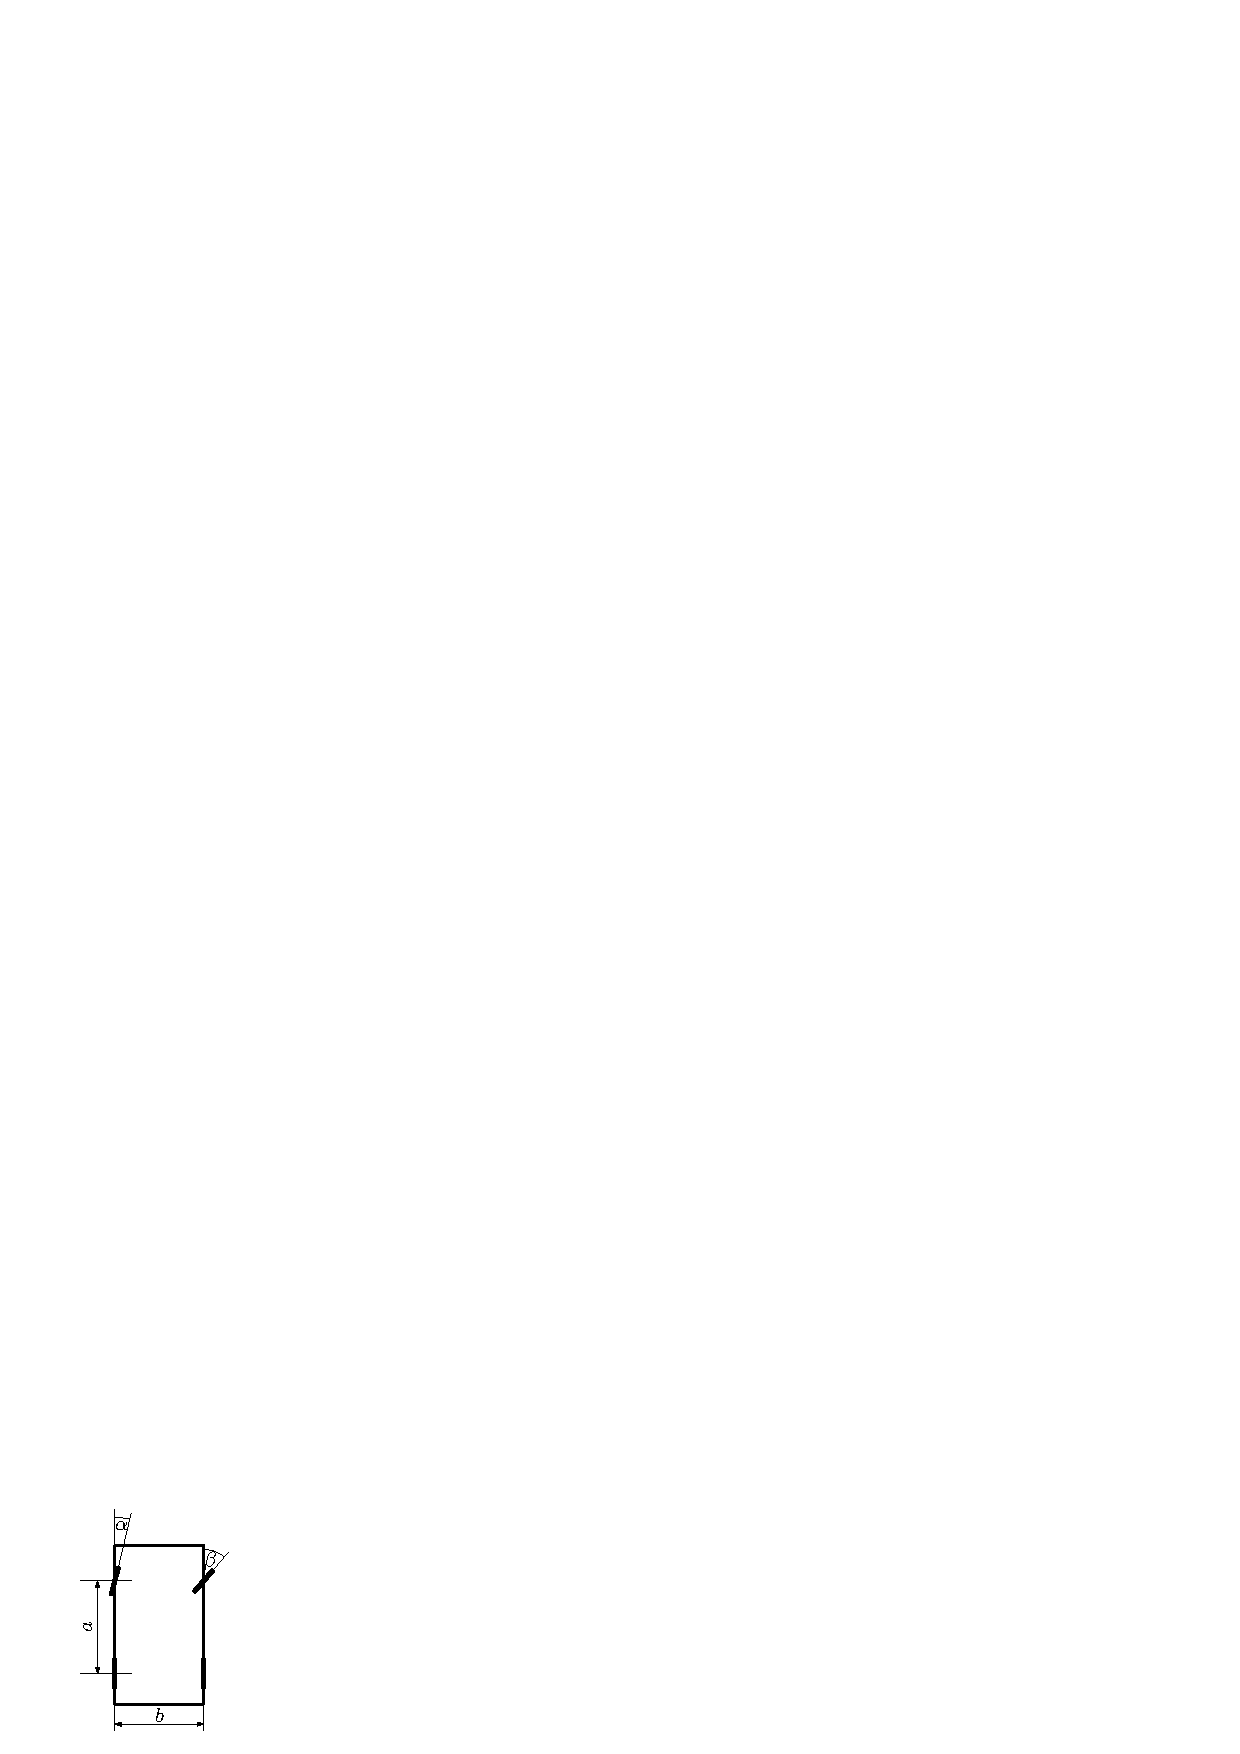
\includegraphics[width=0.3\linewidth]{2012-v3g-05-r_yl_joonis}%
\end{center}
\probend
\bigskip

% Ü135
\setAuthor{Jaan Kalda}
\setRound{lõppvoor}
\setYear{2014}
\setNumber{G 5}
\setDifficulty{6}
\setTopic{Kinemaatika}

\prob{Kammid}
\begin{wrapfigure}{r}{0.6\textwidth}%
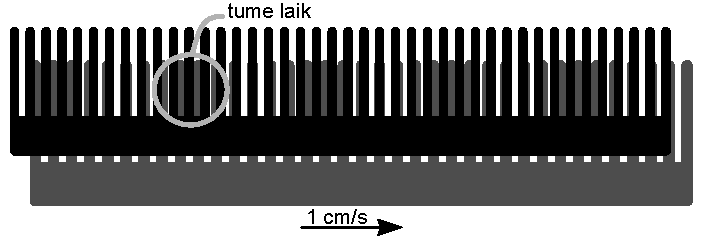
\includegraphics[width=1\linewidth]{2014-v3g-05-kammid}
\end{wrapfigure}

Kaks kammi on asetatud üksteise taha nii, nagu näidatud joonisel. Halli kammi liigutatakse kiirusega $v=\SI 1{cm/s}$ ning musta kammi hoitakse paigal. Millise kiirusega ja millises suunas liiguvad tumedad laigud?
\probend
\bigskip

% Ü136
\setAuthor{Mihkel Kree}
\setRound{lahtine}
\setYear{2014}
\setNumber{G 10}
\setDifficulty{8}
\setTopic{Kinemaatika}

\prob{Päikese pöörlemine}
Maa pöörleb ümber oma telje perioodiga $T_\text{m}\approx\SI{24}{h}$. Ka Päike pöörleb ümber oma telje. Selles võib veenduda näiteks päikeseplekkide liikumist jälgides, aga selles ülesandes kasutame hoopis infot Päikese ketta serval paiknevatest ekvaatori punktidest A ja B kiiratud spektrite kohta. Osutub, et kui mõõdetakse naatriumi kollase neeldumisjoone lainepikkusi, siis punktidest A ja B kiiratud spektritest saadakse selle lainepikkuse jaoks veidi erinevad väärtused. Mõõdetud lainepikkused erinevad teineteisest $\Delta \lambda = \SI{7.8}{pm}=\SI{7.8e-12}{m}$ võrra. Naatriumi kollase neeldumisjoone laboratoorne lainepikkus on $\lambda_0=\SI{590}{nm}$, valguse kiirus $c=\SI{3.0e8}{m/s}$, Päikese raadius $r=\SI{700000}{km}$. Leidke Päikese ekvatoriaalpiirkonna pöörlemisperiood $T_\text{p}$.
\probend
\bigskip

% Ü137
\setAuthor{Jaan Kalda}
\setRound{lõppvoor}
\setYear{2014}
\setNumber{G 9}
\setDifficulty{8}
\setTopic{Kinemaatika}

\prob{Traatrõngad}
Kaks ühesugust traatrõngast raadiusega $R$ on üksteise vahetus läheduses, rõngaste tasandid on paralleelsed ning rõngad puudutavad üksteist punktides $A$ ja $B$. Kaarele $AB$ vastav kesknurk on vaadeldaval ajahetkel $\alpha$. Alumine rõngas on paigal, ülemine pöörleb nurkkiirusega $\omega$ ümber punkti $A$ läbiva ning rõngaste tasanditega risti oleva telje. Leidke rõngaste puutepunkti $B$ kiirus antud ajahetkel.
\probend
\bigskip

% Ü138
\setAuthor{Jaan Kalda}
\setRound{lahtine}
\setYear{2016}
\setNumber{G 9}
\setDifficulty{9}
\setTopic{Kinemaatika}

\prob{Anemomeeter}
Ultraheli anemomeeter mõõdab tuule kiirust sel teel, et määrab aja, mis kulub helisignaalil allikast senosoriteni jõudmiseks.
Olgu heliallikas koordinaatide alguspunktis $O=(0;0)$ ning kolm sensorit punktides koordinaatidega $A=(0;a)$, $B=(a;0)$ ja $C=(-a;0)$, 
kus $a=\SI{211.1}{mm}$ (loeme lihtsustavalt, et nii heliallika kui ka sensorite mõõtmed on tühised). 
Anemomeetrit hoitakse nii, et kõik sensorid paiknevad ühes ja samas horisontaaltasandis ning helisignaali 
sensoriteni jõudmise aegadeks mõõdetakse vastavalt $t_A=\SI{627,0}{\micro s}$, $t_B=\SI{625,2}{\micro s}$ ja $t_C=\SI{603,4}{\micro s}$. 
Milline on tuule kiirus? Arvutustes võite kasutada mõistlikke lihtsustavaid lähendusi.
\probend
\bigskip

% Ü139
\setAuthor{Jaan Kalda}
\setRound{lõppvoor}
\setYear{2016}
\setNumber{G 9}
\setDifficulty{9}
\setTopic{Kinemaatika}

\prob{Kaater}
Kaater sõitis $l=\SI 4{km}$ kaugusel otse lõuna suunas asuvale saarele. 
Alguses võeti suund esimesele meremärgile, seejärel pöörati teise suunas ning lõpuks võeti kurss otse saare peale; seega koosnes trajektoor kolmest sirglõigust. Kaatrilt mõõdeti tuule kiirust ja suunda: esimest lõiku sõideti $t_1=\SI{3}{min}$ ja tuule kiiruseks mõõdeti $v_1=\SI{15}{m/s}$ ning tajutav suund oli otse idast, teist lõiku sõideti $t_2=\SI{1,5}{min}$ ja tuule kiiruseks mõõdeti $v_2=\SI{10}{m/s}$ ning tajutav suund oli otse kagust (lõuna-ida vahelt), kolmandat lõiku sõideti $t_3=\SI{1,5}{min}$ ja tuule kiiruseks mõõdeti $v_3=\SI{5}{m/s}$ ning tajutav suund oli otse edelast (lõuna-lääne vahelt). Mis oli tegelik tuule kiirus?

\emph{Märkus.} Eri lõikudel võis paadi kiirus olla erinev, kuid iga lõigu kestel hoiti konstantne; pööramiseks ja kiirendamiseks kulunud aeg oli tühine; tuule tegelik suund ja kiirus ei muutunud.
\probend
\bigskip
\newpage\subsection{\protect\StrSubstitute{Magnetism}{-}{ }}

% Ü140
\setAuthor{Kristian Kuppart}
\setRound{lahtine}
\setYear{2013}
\setNumber{G 2}
\setDifficulty{3}
\setTopic{Magnetism}

\prob{Magnetpeegel}
Positiivse laenguga $q$ ja kiirusega $v$ osake liigub ristkülikukujulise riba poole nii, et tema kiirusvektor
moodustab riba normaaliga nurga $\alpha$. Riba paksus on $d$ ja seal paikneb
homogeenne $z$-telje suunaline
magnetväli induktsiooniga $B$ (paberi tasandist meie poole suunatud). Millise maksimaalse
langemisnurga $\alpha_{\mathrm{max}}$ korral
osake veel läbib magnetvälja? On teada, et ribaga risti sellesse sisenev osake
läbiks riba.

\begin{center}
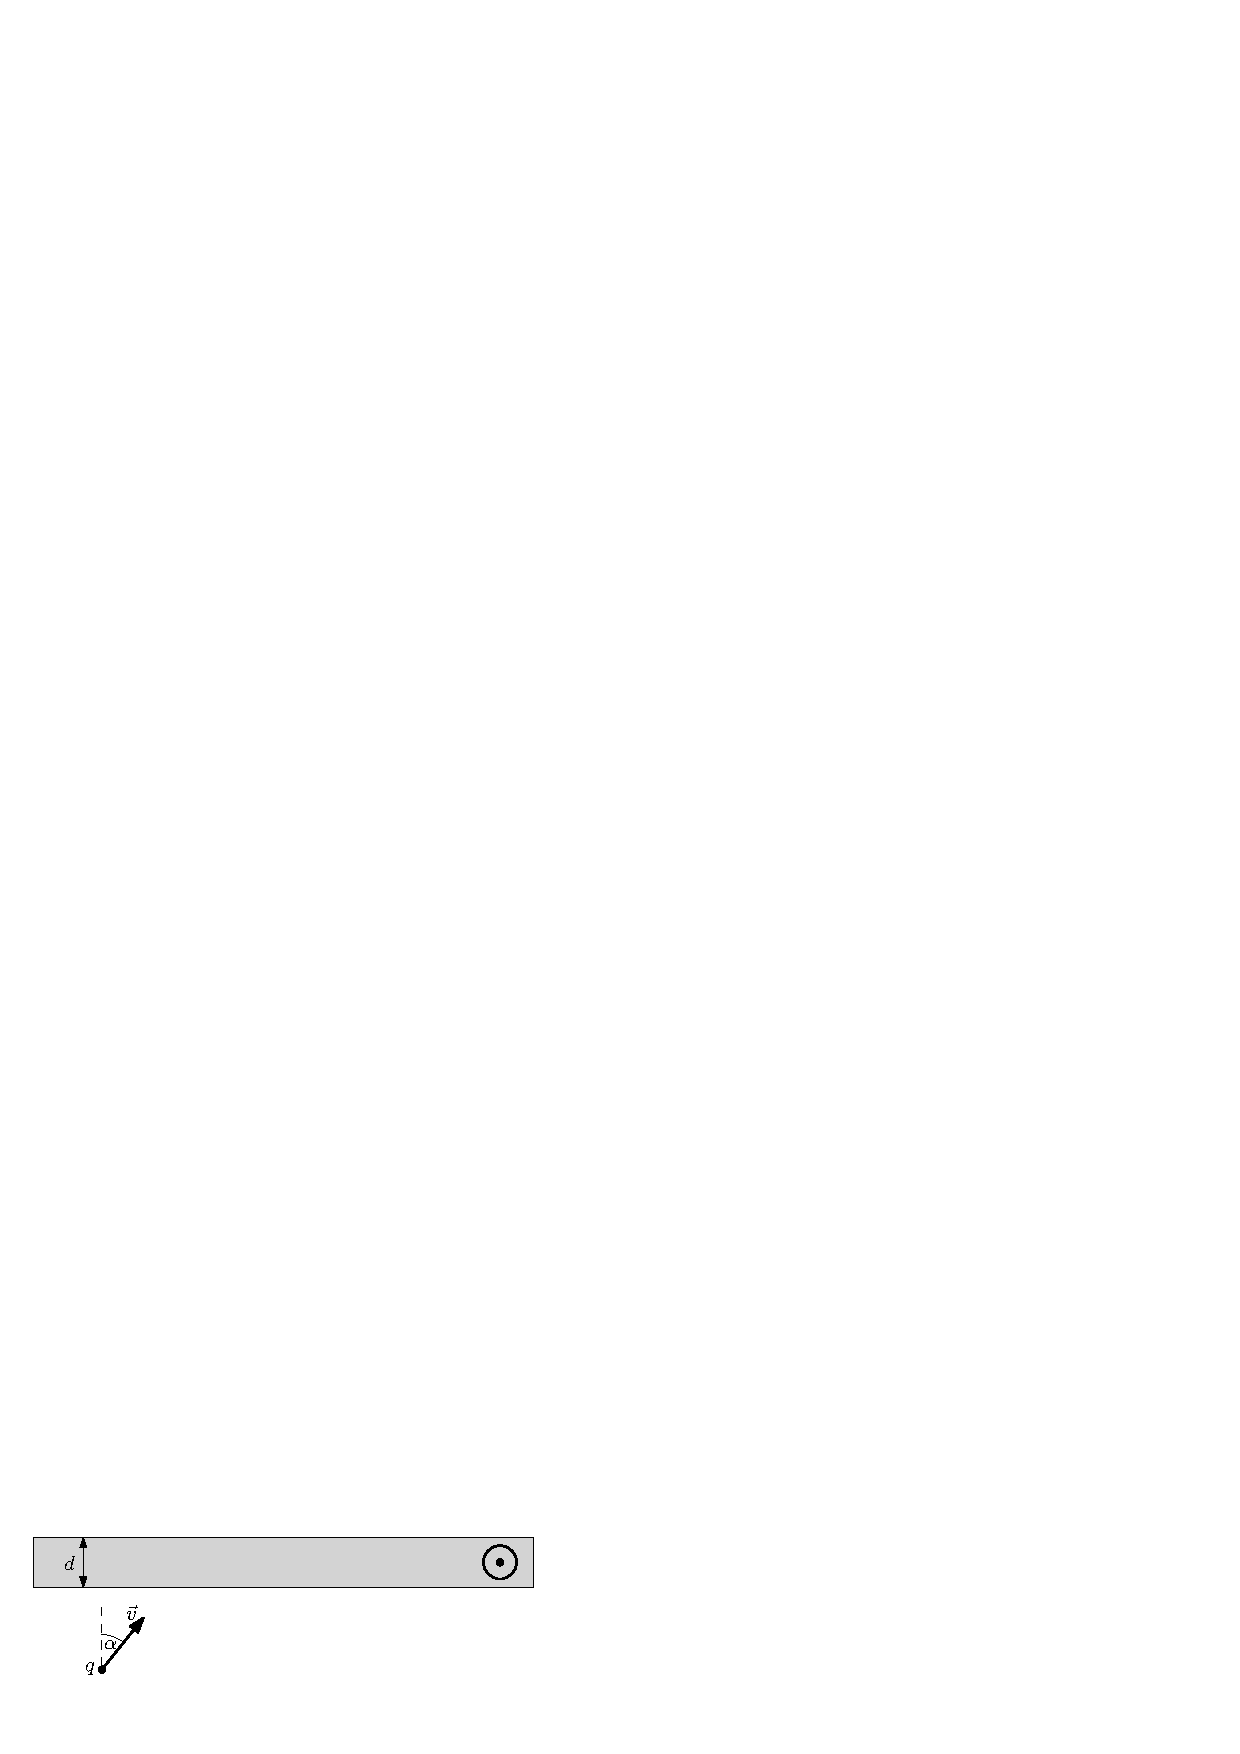
\includegraphics[width=\linewidth]{2013-lahg-02-magnetpeegeljoonis_ipe}
\end{center}
\probend
\bigskip

% Ü141
\setAuthor{Andreas Valdmann}
\setRound{lahtine}
\setYear{2013}
\setNumber{G 5}
\setDifficulty{4}
\setTopic{Magnetism}

\prob{Generaator}
Teatud tüüpi elektrigeneraatoris pöörleb väljundiga ühendatud juhtmekontuur
püsimagnetitega tekitatud magnetväljas, muutes mehaanilise töö elektrienergiaks.
Sellise generaatori külge oli tarbijana ühendatud elektrilamp. Esialgu aeti
generaatorit ringi nurkkiirusega $\omega_0$, mille tulemusel eraldus lambis
võimsus $P_0$. Mingil hetkel suurendati generaatori pöörlemissagedust 2 korda.\\
\osa Kui suur oli lambis eralduv võimsus pärast pöörlemissageduse suurendamist?\\
\osa Kui suur oli generaatori ringiajamiseks tarvilik jõumoment enne ja
pärast pöörlemissageduse suurendamist?

Võib eeldada, et generaator töötas kadudeta ehk kogu tema ringiajamisel tehtav
töö kandus üle tarbijale. Ühtlase sagedusega pöörlemisel on generaatorit
ringiajav jõumoment konstantne. Samuti võib eeldada, et lambi takistus ei sõltu
teda läbiva voolu tugevusest.
\probend
\bigskip

% Ü142
\setAuthor{Eero Vaher}
\setRound{lahtine}
\setYear{2013}
\setNumber{G 6}
\setDifficulty{5}
\setTopic{Magnetism}

\prob{Tiirlev kuulike}
Olgu meil positiivselt laetud kuulike massiga $m$. On teada, et kui kuulike
liiguks kiirusega $v$ sellega ristuvas magnetväljas induktsiooniga $B$,
siis oleks selle trajektooriks ringjoon raadiusega~$r$. Kui suure laenguga $q$ peab olema teine sama massiga kuulike, et esimene
kuulike liiguks teise kuulikese elektriväljas sama kiirusega samal trajektooril? Eeldage, et
kahe kuulikese süsteemile ei mõju väliseid jõude. Kõiki liikumisi vaadeldakse
laboratoorses taustsüsteemis.
\pagebreak
\probend
\bigskip

% Ü143
\setAuthor{Kristian Kuppart}
\setRound{piirkonnavoor}
\setYear{2018}
\setNumber{G 10}
\setDifficulty{6}
\setTopic{Magnetism}

\prob{Tsüklotron}
\begin{wrapfigure}{r}{0.35\linewidth}
	\begin{center}
		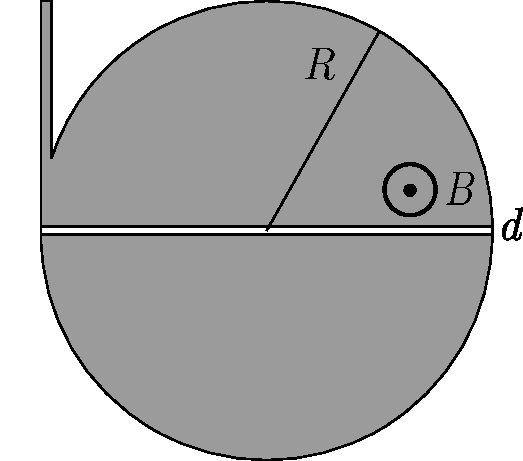
\includegraphics[width=\linewidth]{2018-v2g-10-tsyklotron}
	\end{center}
\end{wrapfigure}

Vaatleme tsüklotroni -- teatud tüüpi osakestekiirendi toimimist. Tsüklotron koosneb silindrikujulisest piirkonnast raadiusega $R$, kus on homogeenne magnetväli tugevusega $B$, ning õhukesest ribakujulisest piirkonnast laiusega $d$, kus on homogeenne ribaga risti olev elektriväli tugevusega $E$. Elektrivälja suunda muudetakse perioodiliselt vastassuunaliseks nii, et osakeste igal riba läbimisel on elektrivälja suund osakeste kiirusvektoriga samasuunaline. Samuti on tsüklotroni ühes ääres osakeste tsüklotronist väljumiseks kitsas kanal. Alustagu osakesed liikumist tsüklotroni keskelt tühiselt väikse algkiirusega. Mitu täisringi $n$ teevad osakesed tsüklotronis enne väljumist? Osakeste laeng on $q$ ja mass $m$. Eeldada, et $n\gg 1.$
\probend
\bigskip

% Ü144
\setAuthor{Kristian Kuppart}
\setRound{piirkonnavoor}
\setYear{2013}
\setNumber{G 10}
\setDifficulty{7}
\setTopic{Magnetism}

\prob{Mass-spektromeeter}
\begin{wrapfigure}[4]{r}{3cm}%
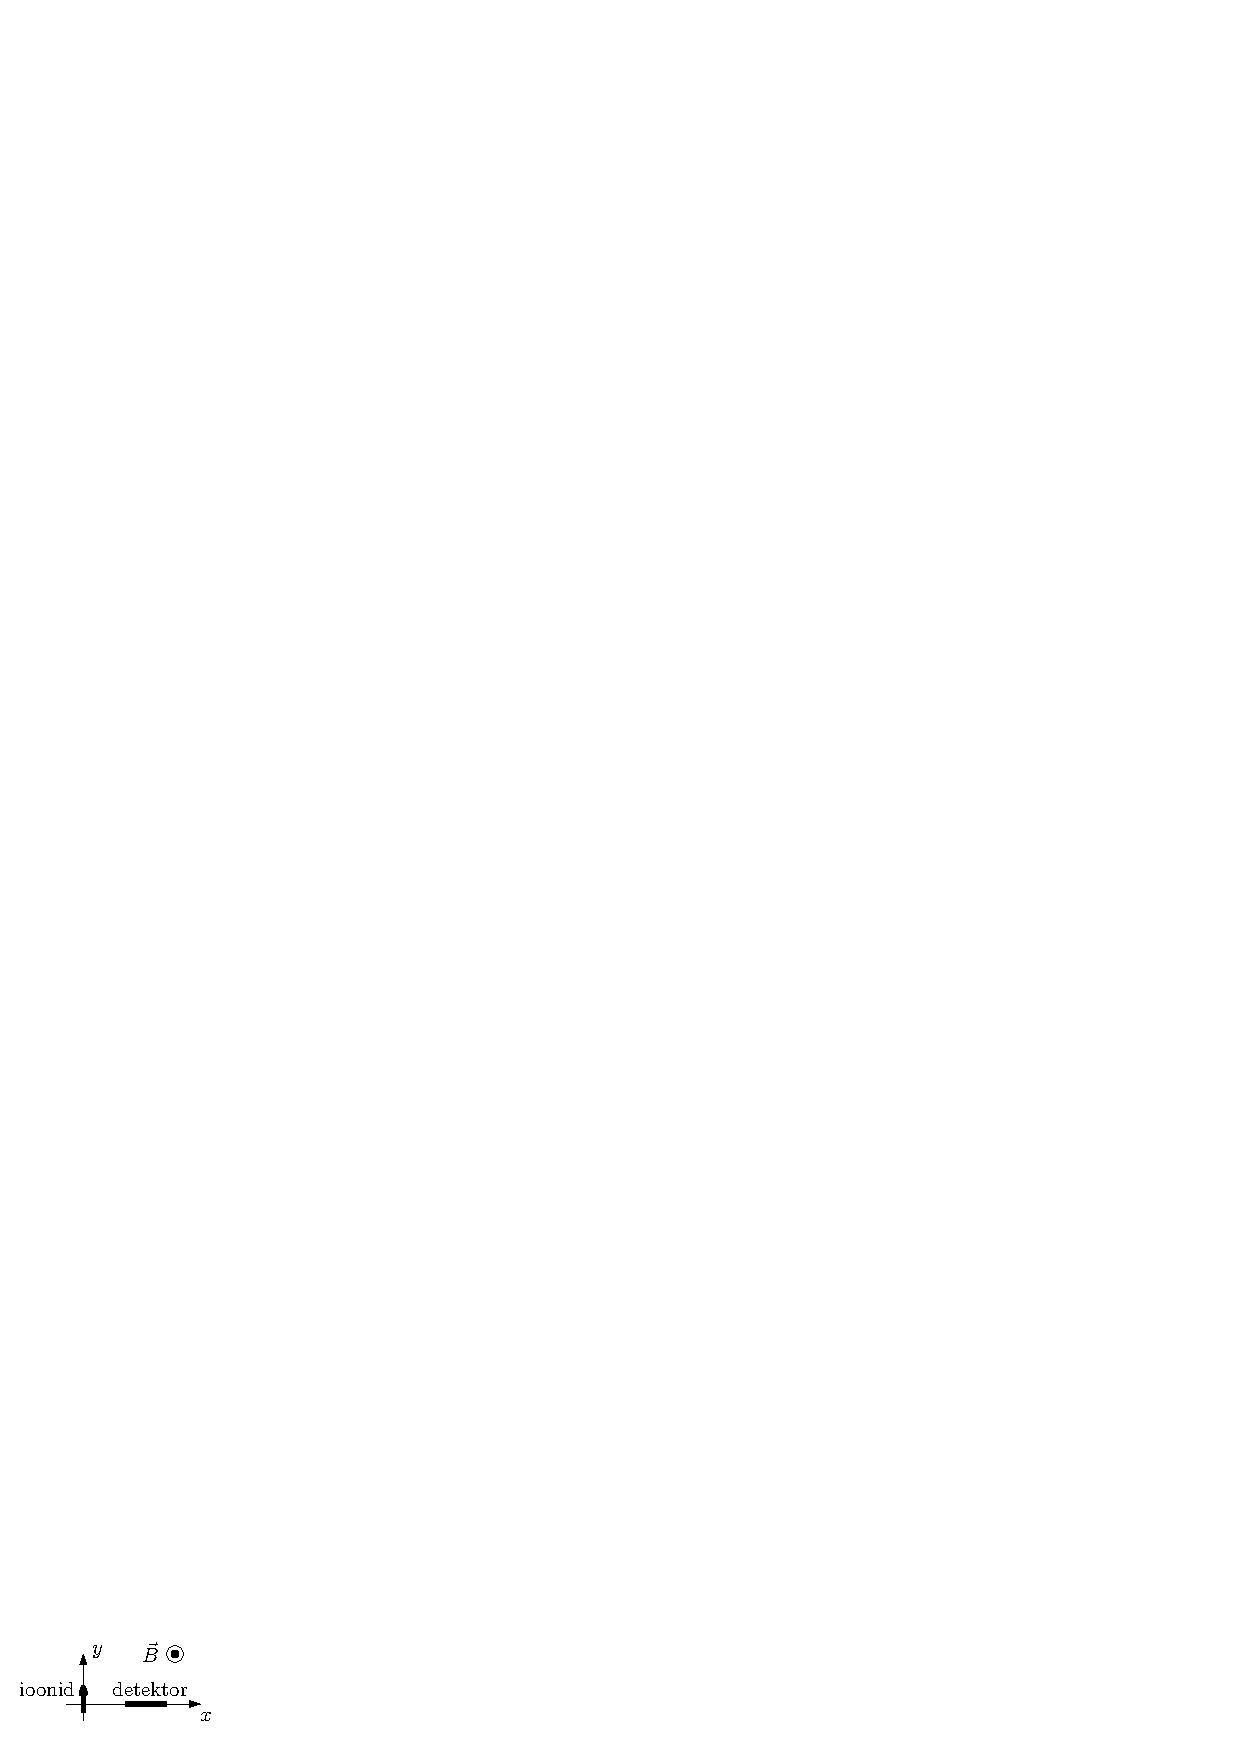
\includegraphics[width=\linewidth]{2013-v2g-10-massspektromeeter_ipe}%
\end{wrapfigure}
Laboris oli uurimiseks hulk mingit atomaarset ainet, mille molaarmassiks mõõdeti
$\mu_{1}$. Ühekordselt ioniseeritud ainet (iga aatom oli kaotanud ühe
elektroni) kiirendati elektriväljas potentsiaalide vahega $U$ ja suunati magnetvälja
induktsiooniga $B$ (vaadake joonist). Magnetinduktsioon oli joonise tasandiga
risti, 
ioonide algkiirus oli $y$-telje suunaline,
magnetväli asus piirkonnas $y>0$ ning aine sisenes magnetvälja punktis
$(0, 0, 0)$.

Täheldati, et väike kogus ainet langes $x$-teljel asuvale
detektorile kauguse
$d$ võrra kaugemal kohast, kuhu langes põhiosa ainest. Sellest järeldati,
et aine hulgas oli väike osa isotoopi erineva molaarmassiga. Leidke
selle isotoobi molaarmass $\mu_{2}$. Avogadro arv on $N_A$ ja elektroni laeng
on $-e$.
\probend
\bigskip

% Ü145
\setAuthor{Jaan Kalda}
\setRound{piirkonnavoor}
\setYear{2015}
\setNumber{G 9}
\setDifficulty{8}
\setTopic{Magnetism}

\prob{Magnetväli}
Piirkonnas $0<y<a$ on $z$-teljega paralleelne homogeenne magnetväli induktsiooniga $B$; piirkondades $y<0$ ja $y>a$ magnetväli puudub. 
Osake massiga $m$ ja laenguga $q$ siseneb kiirusega $v$ magnetväljaga piirkonda paralleelselt $y$-teljega üle joone $y=0$. Visandage osakese kiirusvektori ja $y$-telje vaheline nurk pärast seda, kui osake on piirkonnast $0<y<a$ väljunud funktsioonina kiirusest $v$.
\probend
\bigskip

% Ü146
\setAuthor{Eero Vaher}
\setRound{lahtine}
\setYear{2015}
\setNumber{G 10}
\setDifficulty{9}
\setTopic{Magnetism}

\prob{Laetud pendel}
Väike laetud kuulike massiga $m$ ja laenguga $q$ ripub venimatu pikkusega $l$ niidi otsas magnetväljas induktsiooniga $B$. Kuulike viiakse niiti sirgena hoides kõrgusele $H=\frac{7}{8}l$ ning lastakse siis lahti. Raskuskiirendus on $g$ ning magnetvälja suund on risti pendli võnketasandiga. Samuti on teada, et kehtib $q^2B^2l=\frac{3}{4}m^2g$. Milline on kuulikese trajektoor?

\begin{center}
\begin{resizebox}{0.5\linewidth}{!}{
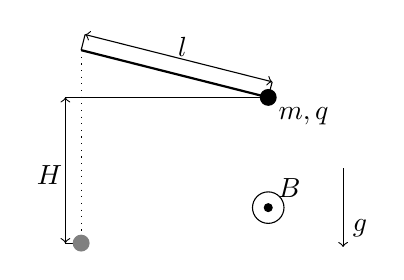
\begin{tikzpicture}
\newcommand{\x}{1.2*1.98}
\newcommand{\y}{-0.6}
\newcommand{\length}{{veclen(\x,\y)}}

\draw (\x,-2) circle (0.2) node [above right] {$B$};
\draw[fill=black] (\x, -2) circle (0.05);
\draw[->] (1.4*\x,-1.5) -- (1.4*\x,-2.5) node[above right] {$g$};

\draw[<->] (0.05,-0.05*\x/\y) -- (\x+0.05,\y-0.05*\x/\y);
\draw (0,0) -- (0.05,-0.05*\x/\y);
\draw (\x,\y) -- (\x+0.05,\y-0.05*\x/\y);
\draw[thick] (0,0) -- (\x,\y) node[below right] {$m,q$};
\draw[fill=black] (\x,\y) circle (0.1);
\node[above] at (\x/2+0.1,\y/2+0.1) {$l$};

\draw[<->] (-0.2,\y) -- (-0.2,-\length);
\draw (\x,\y) -- (-0.2,\y);
\draw (0,-\length) -- (-0.2,-\length);
\draw[dotted] (0,0) -- (0,-\length);
\draw[gray, fill=gray] (0,-\length) circle (0.1);
\node[left] at (0,-\length/2.5+\y) {$H~$};
\end{tikzpicture}}
\end{resizebox}
\end{center}
\probend
\bigskip

% Ü147
\setAuthor{Jaan Kalda}
\setRound{lõppvoor}
\setYear{2017}
\setNumber{G 10}
\setDifficulty{10}
\setTopic{Magnetism}

\prob{Elektronid}
Ruumipiirkonnas $x>-a$ ($a>0$) on homogeenne $z$-telje sihiline magnetväli induktsiooniga $B$. 
Koordinaatide alguspunktis on elektronide allikas, mis kiirgab elektrone võrdsel arvul
kõikidesse suundadesse (üle ruuminurga $4\pi$). Kõikide elektronide kiirus on $v$. Tasandis $x=-a$ on ekraan. Kui elektronid 
laenguga $e$ ja massiga $m$ põrkuvad vastu 
ekraani, siis on kokkupõrkepunktis näha helendust. Leidke helenduva laigu $y$-telje sihiline
läbimõõt tasandil $z = 0$ eeldusel, et vähemalt osa elektronidest jõuavad ekraanini.
Samal tasandil leida, kus kohas on laigu helenduse intensiivsus
kõige suurem. Milline on selle laigu $z$-telje sihiline pikkus tasandil $y=0$?
\probend
\bigskip
\newpage\subsection{\protect\StrSubstitute{Staatika}{-}{ }}

% Ü148
\setAuthor{Taavi Pungas}
\setRound{piirkonnavoor}
\setYear{2014}
\setNumber{G 6}
\setDifficulty{4}
\setTopic{Staatika}

\prob{Rõngas}
Lae külge on nööriga, mille pikkus on $L$, kinnitatud kerge plastmassrõngas raadiusega $R$, mille küljes on omakorda raske metallist mutter. Mutrit saab mööda rõngast libistada. Rõnga ja mutri vaheline hõõrdetegur on $\mu$. Juku tahab mutrit mööda rõngast nihutades saavutada olukorda, kus mutri ja lae vahekaugus $h$ oleks võimalikult väike, aga süsteem püsiks veel ilma välise sekkumiseta tasakaalus. Leidke vähim vahekaugus $h\idx{min}$, mille Juku võib saavutada. Eeldage, et rõnga mass on mutri omaga võrreldes tühiselt väike.
\probend
\bigskip

% Ü149
\setAuthor{Mihkel Rähn}
\setRound{piirkonnavoor}
\setYear{2015}
\setNumber{G 7}
\setDifficulty{5}
\setTopic{Staatika}

\prob{Poldilõikur}
Leida, kui suurt jõudu avaldab poldilõikuri tera poldile (vt joonis), kui käepidemetele avaldatud jõud on $F = \SI{90}{N}$.
 \begin{center}
 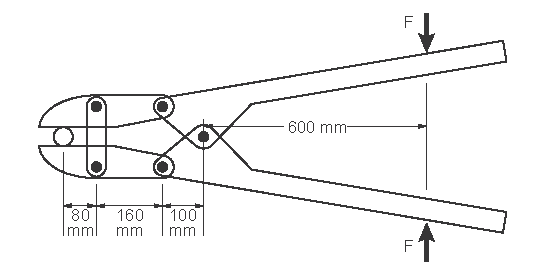
\includegraphics[width=0.7\textwidth]{2015-v2g-07-poldiloikur}
 \end{center}
\probend
\bigskip

% Ü150
\setAuthor{Mihkel Rähn}
\setRound{piirkonnavoor}
\setYear{2014}
\setNumber{G 7}
\setDifficulty{6}
\setTopic{Staatika}

\prob{Klotsid}
Horisontaalsel laual asuva klotsi massiga $m_1$ peale on asetatud teine klots massiga $m_2$. Kahe klotsi vaheline seisuhõõrdetegur on $\mu_2$. Alumise klotsi ja laua vaheline liugehõõrdetegur on $\mu_1$. Leidke maksimaalne horisontaalne jõud $F$, millega võib alumist klotsi tõmmata, ilma et ülemine klots libiseks.
\probend
\bigskip

% Ü151
\setAuthor{Mihkel Rähn}
\setRound{lõppvoor}
\setYear{2014}
\setNumber{G 6}
\setDifficulty{6}
\setTopic{Staatika}

\prob{Polüspast}
Jäälõhesse kukkunud alpinisti väljatõmbamiseks on käepärastest vahenditest (kolm plokki ja nöörijupid) koostatud polüspast. Lihtsustatud joonisel on jämeda joonega märgitud põhiköis, mille ühes otsas on kukkunu ning teisest otsast vinnatakse. Plokid on peene joonega kujutatud nööri abil kinnitatud mittelibiseva sõlmega (joonisel täidetud ring) põhiköie külge. Leidke polüspasti ülekandetegur nii hõõrdumist arvestamata kui ka eeldusel, et hõõrdumine vähendab jõuülekannet igal plokil $\SI{35}{\percent}$. Eeldage, et kõik jõud on vertikaalsed.

\begin{center}
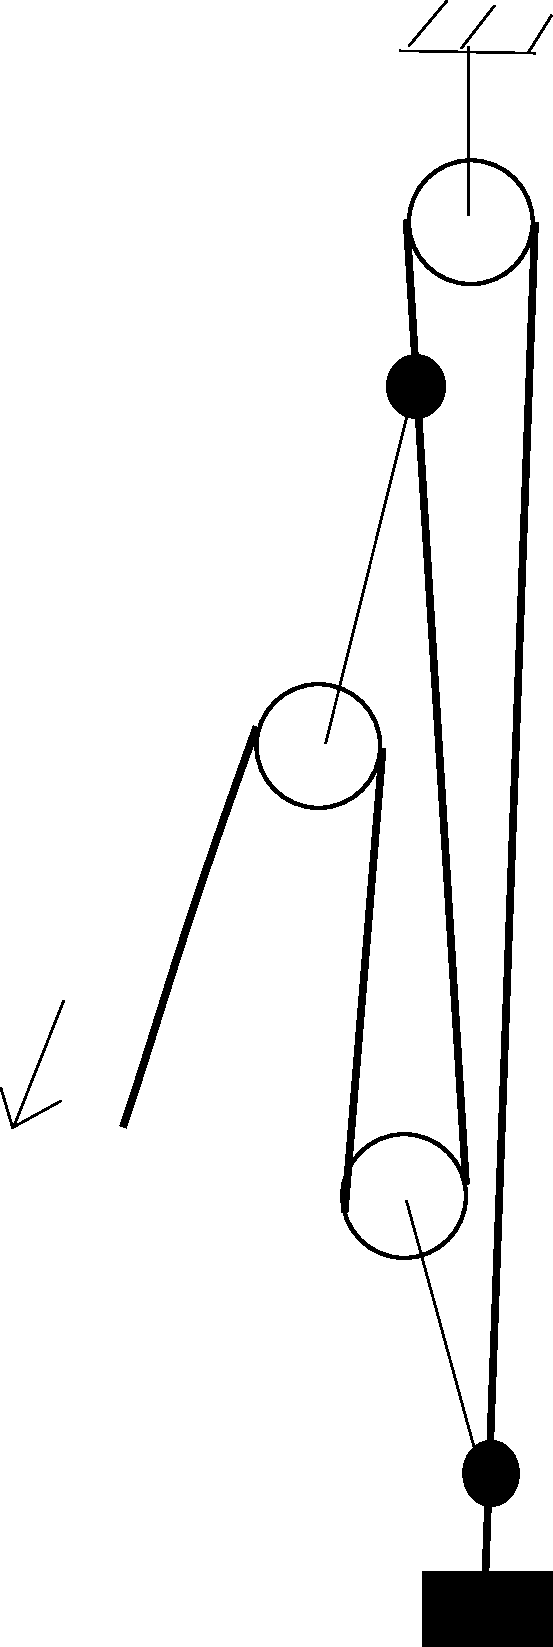
\includegraphics[width=0.25\linewidth]{2014-v3g-06-Polyspast}
\end{center}
\probend
\bigskip

% Ü152
\setAuthor{Andreas Valdmann}
\setRound{piirkonnavoor}
\setYear{2018}
\setNumber{G 9}
\setDifficulty{6}
\setTopic{Staatika}

\prob{Kelk}
Juku läks sõpradega kelgutama. Teel tagasi istusid Juku kaks sõpra kelgule ja Juku üritas kelku horisontaalsel lumisel teel enda järel vedada. Kui suur on minimaalne kelgunööri nurk maapinnaga, mille korral on Jukul võimalik kelk liikuma tõmmata? Juku mass $m_1 = \SI{60}{kg}$ ja hõõrdetegur Juku saabaste ning lume vahel $\mu_1 = \SI{0.30}{}$. Kelgu mass koos Juku sõpradega $m_2 = \SI{110}{kg}$ ja hõõrdetegur kelgu ning lume vahel $\mu_2 = \SI{0.20}{}$.
\probend
\bigskip

% Ü153
\setAuthor{Mihkel Kree}
\setRound{lahtine}
\setYear{2013}
\setNumber{G 8}
\setDifficulty{7}
\setTopic{Staatika}

\prob{Niidirull}
\begin{wrapfigure}[6]{r}{3cm}
\vspace{-15pt}
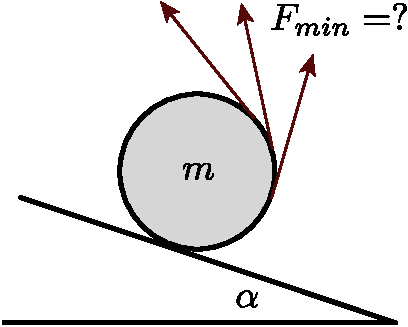
\includegraphics[width=\linewidth]{2013-lahg-08-joonis_niidirull-crop}
\end{wrapfigure}

Silinder massiga $m$, millele on keritud õhuke niit, asetatakse kaldpinnale nurgaga $\alpha$.
Millise minimaalse jõuga $F\idx{min}$ tuleb nöörist hoida, et silinder paigale
jääks (vt joonist)? Hõõrdetegur pinna ja silindri vahel on nii suur, et
libisemist ei toimu.
\probend
\bigskip

% Ü154
\setAuthor{Andres Põldaru}
\setRound{lahtine}
\setYear{2014}
\setNumber{G 8}
\setDifficulty{7}
\setTopic{Staatika}

\prob{Jalgrattur}
Jalgrattur sõidab alla ühtlase kallakuga nõlvast. Kui ta vajutab pidureid täpselt nii kõvasti, et tagumine ratas on peaaegu õhku tõusmas, siis tema kiirus mäest alla sõites ei muutu. Jalgratturist ja rattast koosneva süsteemi massikese asub täpselt kahe ratta vahel kaugusel $h$ maapinnast, rataste telgede vahekaugus on $d$. Kui suur on nõlva ja horisontaalsihi vaheline nurk $\alpha$? Kui suur peab olema ratta ja kaldpinna vaheline hõõrdetegur $\mu$, et jalgrattur saaks kirjeldatud moel pidurdada?
\probend
\bigskip

% Ü155
\setAuthor{Stanislav Zavjalov}
\setRound{lahtine}
\setYear{2012}
\setNumber{G 9}
\setDifficulty{9}
\setTopic{Staatika}

\prob{Nöör rennis}
\begin{wrapfigure}{r}{0.4\linewidth}
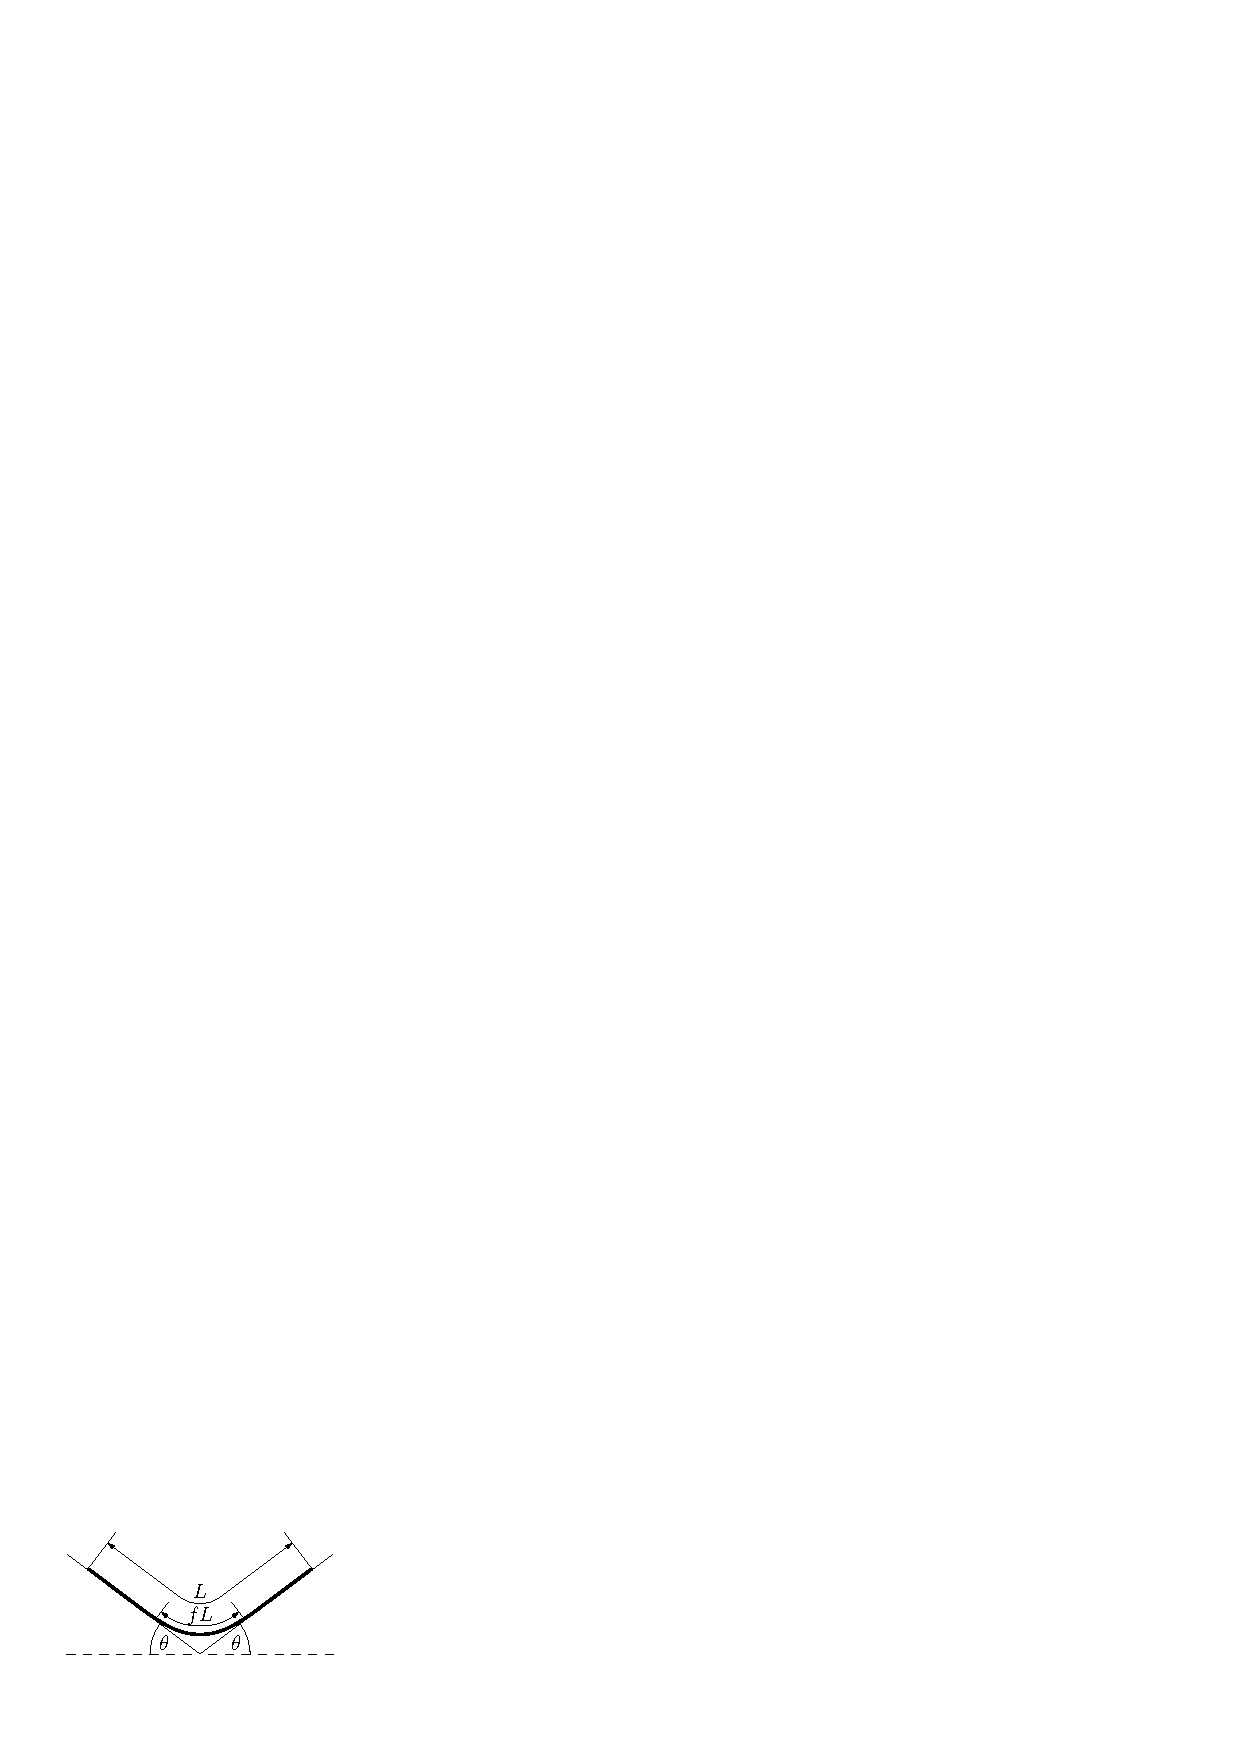
\includegraphics[width=\linewidth]{2012-lahg-09-n88r_ipe}
\end{wrapfigure}
Kaks plaati moodustavad V-kujulise horisontaalse renni. Mõlemad plaadid on
horisontaaltasapinna suhtes nurga $\theta$ all.
Rennis on jupp ühtlase
massijaotusega nööri pikkusega $L$, mis asub tervikuna renniga ristuvas tasandis
nii, et mõlema plaadiga puutub kokku sama palju nööri.
Renni põhja kohal ei toetu nöör enam pikkuse $fL$
ulatuses plaatidele. Leidke $f$, kui nöör on libisemise piiril. Hõõrdetegur nööri ja plaatide
vahel on $\mu = 1$.
\probend
\bigskip

% Ü156
\setAuthor{Jaan Kalda}
\setRound{lõppvoor}
\setYear{2017}
\setNumber{G 9}
\setDifficulty{9}
\setTopic{Staatika}

\prob{Katus}
Kaks jäika traadijuppi pikkusega $L$ on ühendatud otsapidi (nt niidiga seotud) nii, et nende otspunktid on kontaktis ja nende vaheline nurk saab takistuseta muutuda, moodustades V-kujulise figuuri. See traadist moodustis asetatakse horisontaalse libedapinnalise silindri peale nõnda, et tasakaaluasendis moodustub traadist \enquote{katus} (tagurpidi \enquote{V}) tipunurgaga $\alpha$. Massijaotus traadis on ühtlane, hõõre traadi ja silindri vahel puudub. a) Milline on silindri raadius $R$? b) Milline võrratus peab olema rahuldatud, et see asend oleks stabiilne (uurida stabiilsust vaid \enquote{katuse} kui terviku pöördumise suhtes, eeldades et traatidevaheline nurk ei muutu)?
\probend
\bigskip

% Ü157
\setAuthor{Jaan Kalda}
\setRound{lõppvoor}
\setYear{2015}
\setNumber{G 9}
\setDifficulty{10}
\setTopic{Staatika}

\prob{Niidiga hantel}
\begin{wrapfigure}{r}{0.23\textwidth}%
\vspace{-5 pt}%
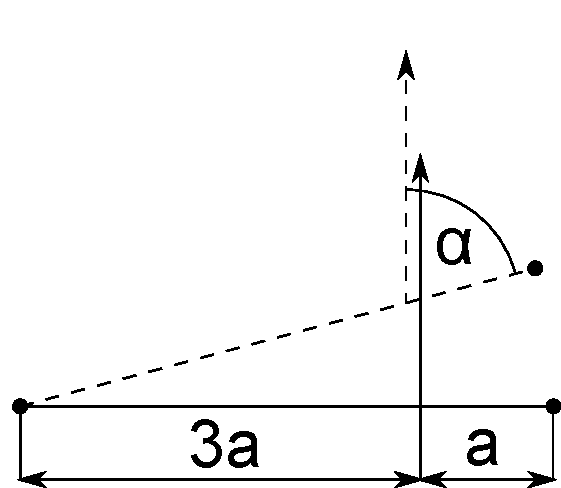
\includegraphics[width=0.23\textwidth]{2015-v3g-09-hantel}%
\vspace{-15 pt}%
\end{wrapfigure}
Horisontaalpinnal lebab hantel, mis koosneb kaalutust vardast pikkusega $l=4a$ ning selle otstele kinnitatud kahest ühesuguse massi ja hõõrdeteguriga väikesest klotsist. Varda külge kaugusele $a$ ühest klotsist on seotud pikk niit. Algul on niidi suund horisontaalne ja risti vardaga. Niiti aeglaselt tõmmates hakkab hantel pöörduma, sest alguses nihkub vaid üks klots. Milline on nurk $\alpha$ varda ja niidi vahel siis, kui ka teine klots nihkuma hakkab?
\probend
\bigskip
\newpage\subsection{\protect\StrSubstitute{Taevamehaanika}{-}{ }}

% Ü158
\setAuthor{Eero Vaher}
\setRound{piirkonnavoor}
\setYear{2014}
\setNumber{G 3}
\setDifficulty{2}
\setTopic{Taevamehaanika}

\prob{Maa pöörlemisperiood}
Keskmiseks päikeseööpäevaks ehk tavatähenduses ööpäevaks nimetatakse keskmist perioodi, mille jooksul Päike näib Maaga seotud vaatleja jaoks tegevat taevas täisringi. Keskmise päikeseööpäeva pikkuseks on \SI{24}{\hour} ehk \SI{86400}{\second}. Maal kulub ühe tiiru tegemiseks ümber Päikese \SI{365.256}{} keskmist päikeseööpäeva. Maa pöörlemissuund ümber oma telje ühtib selle tiirlemissuunaga Päikese ümber. Leidke nende andmete põhjal Maa pöörlemisperiood sekundi täpsusega.
\probend
\bigskip

% Ü159
\setAuthor{Mihkel Pajusalu}
\setRound{lahtine}
\setYear{2014}
\setNumber{G 3}
\setDifficulty{3}
\setTopic{Taevamehaanika}

\prob{Orbiit}
Taevakehad tiirlevad teatavasti elliptilistel orbiitidel. Ka Kuu orbiit ümber Maa on elliptiline. Kui Kuu kõige väiksem kaugus Maa-Kuu süsteemi massikeskmest (mille selles ülesandes võib lugeda ühtivaks Maa keskpunktiga) on $r_{1}=\SI{360000}{km}$ ja orbitaalkiirus sellel kaugusel on $v_1=\SI{1.1}{km/s}$, siis kui suur on ligikaudu suurim kaugus Maa ja Kuu vahel? Maa massiks võtta $M=\SI{6.0e24}{kg}$ ja gravitatsioonikonstandiks $G=\SI{6.7e-11}{\newton\metre\squared\per\kilo\gram\squared}$.
\probend
\bigskip

% Ü160
\setAuthor{Eero Vaher}
\setRound{piirkonnavoor}
\setYear{2013}
\setNumber{G 6}
\setDifficulty{4}
\setTopic{Taevamehaanika}

\prob{Päikese tihedus}
Leidke Päikese keskmine tihedus $\varrho$. Maa
tiirlemisperiood on $T=1$~aasta, gravitatsioonikonstant 
$G=\SI{6.7e-11}{N m^2/kg^2}$, Maa kaugus Päikesest $R=\SI{1.5e11}{m}$, Päikese nurkläbimõõt Maalt vaadatuna on
$\alpha=\ang{0,54}$ (see on nurk, mis moodustub kahe kiire vahel, mis on tõmmatud
vaatleja silma juurest Päikese diameetri otspunktide juurde).
\probend
\bigskip

% Ü161
\setAuthor{Eero Vaher}
\setRound{piirkonnavoor}
\setYear{2018}
\setNumber{G 6}
\setDifficulty{4}
\setTopic{Taevamehaanika}

\prob{Ühendatud satelliidid}
Kaks satelliiti, mõlemad massiga $m$, tiirlevad ümber planeedi massiga $M\gg m$ ringorbiitidel raadiustega $R_1$ ning $R_2=2R_1$. Satelliidid on omavahel ühendatud tühise massiga pinges trossiga pikkusega $R_1$, mille tõttu on mõlema satelliidi tiirlemisperiood $T$. Mitu korda on satelliitide joonkiirused $v_1$ ja $v_2$ suuremad või väiksemad joonkiirustest $v'_1$ ja $v'_2$, millega satelliidid tiirleksid oma orbiitidel trossi puudumisel?
\probend
\bigskip

% Ü162
\setAuthor{Eero Vaher}
\setRound{lõppvoor}
\setYear{2013}
\setNumber{G 5}
\setDifficulty{5}
\setTopic{Taevamehaanika}

\prob{Satelliit}
Geostatsionaarseks orbiidiks nimetatakse sellist orbiiti, millel asuv satelliit
Maa suhtes ei liigu. Kui suur on maa-ala, mida sellisel orbiidil olevalt
satelliidilt jälgida saab? Vastuseks esitage selle maa-ala läbimõõt mõõdetuna
mööda Maa pinda. Gravitatsioonikonstant $G=\SI{6.7e-11}{N \cdot m^2/kg^2}$, Maa
mass $M=\SI{6,0e24}{kg}$, Maa raadius $r=\SI{6400}{km}$, Maa
pöörlemisperiood $t=\SI{24}{h}$.
\probend
\bigskip
\newpage\subsection{\protect\StrSubstitute{Termodünaamika}{-}{ }}

% Ü163
\setAuthor{Jaak Kikas}
\setRound{lahtine}
\setYear{2012}
\setNumber{G 1}
\setDifficulty{1}
\setTopic{Termodünaamika}

\prob{Vee jäätumine}
\SI{0,5}{\kilo\gram} jääkuubikuid asetati \SI{1}{l} vette algtemperatuuriga
\SI{0}{\degreeCelsius}. Milline peab olema jää algtemperatuur, et kogu vesi jäätuks?
Jää sulamissoojus on \SI{330}{\kilo\joule\per\kilo\gram}, erisoojus
\SI{2,1}{\kilo\joule\per(\kilogram.\degreeCelsius)}. Soojusvahetust keskkonnaga ei
toimu.
Vee tihedus $\rho = \SI{1000}{kg/m^3}$.
\probend
\bigskip

% Ü164
\setAuthor{Koit Timpmann}
\setRound{piirkonnavoor}
\setYear{2013}
\setNumber{G 2}
\setDifficulty{1}
\setTopic{Termodünaamika}

\prob{Veepudel}
Külma ilmaga oli autosse ununenud \num{2,0}-liitrine täis veepudel. Auto juurde tulnud
autojuht Koit ei uskunud oma silmi: temperatuur autos oli \SI{-3}{\degreeCelsius},
aga vesi pudelis ei olnud külmunud. Koidule tuli meelde, et ta oli kunagi
kuulnud, et väga puhas vedelik võib olla vedelas olekus ka allpool
tahkumistemperatuuri. Selle kontrollimiseks võttis ta pudeli ja raputas seda
ning suhteliselt kiiresti muutus selles osa veest jääks. Mitu grammi jääd tekkis
pudelisse? Vee erisoojus $c = \SI{4200}{\joule\per(\kilogram \cdot \degreeCelsius)}$
ja tihedus $\varrho = \SI{1000}{\kilogram\per\meter\cubed}$, jää
sulamissoojus $\lambda = \SI{340}{ kJ/kg}$.
\probend
\bigskip

% Ü165
\setAuthor{Ants Remm}
\setRound{lõppvoor}
\setYear{2012}
\setNumber{G 1}
\setDifficulty{2}
\setTopic{Termodünaamika}

\prob{Hõõrdkeevitus}
Suhteliselt uus keevitustehnoloogia on hõõrdkeevitus. See seisneb selles, et üks
liidetavatest detailidest pannakse pöörlema ning surutakse vastu teist. Kui
tekkinud soojus on detailid peaaegu sulamistemperatuurini kuumutanud, jäetakse
pöörlev detail seisma ning suure rõhu all moodustub side. Vaatame olukorda, kus
kaks vasest torujuppi tahetakse kokku keevitada. Leidke, kui suure jõuga peab
pöörlemise ajal torusid kokku suruma, et tekiks piisavalt suur soojushulk
$\Delta t = \SI{6}{s}$ jooksul. Toru pöörlemiskiirus on $f = 1200$ pööret
minutis. Lihtsustatult võib eeldada, et mõlema toru otsast kuumeneb ühtlaselt $l
= \SI{0,5}{cm}$ pikkune jupp. Torude diameeter on $D = \SI{8}{cm}$, seina paksus
$d = \SI{5}{mm}$. Torud on alguses toatemperatuuril $T_0 = \SI{20}{^\circ C}$.
Liitumine toimub temperatuuril $T_1 = \SI{810}{^\circ C}$. Vase hõõrdetegur
iseendaga on $\mu = 0,96$, tihedus $\rho = \SI{8,9}{\frac{g}{cm^3}}$ ning
erisoojus $c = \SI{390}{\frac{J}{kg \cdot \degreeCelsius}}$. Soojuskadudega ümbritsevasse
keskkonda mitte arvestada.
\probend
\bigskip

% Ü166
\setAuthor{Erkki Tempel}
\setRound{piirkonnavoor}
\setYear{2015}
\setNumber{G 3}
\setDifficulty{2}
\setTopic{Termodünaamika}

\prob{Münt jääs}
Jäätüki sisse on jäätunud münt massiga $m_m=\SI{10}{g}$ ja tihedusega $\rho_m=\SI{8900}{kg/m^3}$. Jäätüki ja mündi temperatuur on \SI{0}{\degreeCelsius}. Jäätükk ilma mündita kaalub $m_j=\SI{130}{g}$. See jäätükk visatakse anumasse, milles on $V_v=\SI{400}{ml}$ vett algtemperatuuriga $T$. Kui suur peab olema vee minimaalne algtemperatuur $T$, et jäätükk koos mündiga vajuks pärast soojusliku tasakaalu saabumist põhja? Soojusvahetust väliskeskkonnaga mitte arvestada. Vee erisoojus $c=\SI{4200}{J/ (kg\cdot\degreeCelsius)}$ ning jää sulamissoojus $\lambda=\SI{330}{kJ/kg}$. Jää tihedus $\rho_j=\SI{900}{kg/m^3}$ ja vee tihedus $\rho_v=\SI{1000}{kg/m^3}$.
\probend
\bigskip

% Ü167
\setAuthor{Kaur Aare Saar}
\setRound{lõppvoor}
\setYear{2016}
\setNumber{G 1}
\setDifficulty{2}
\setTopic{Termodünaamika}

\prob{Soojusvaheti}
Tagasivoolu soojusvahetis jahutatakse sissetulevat naftat temperatuuriga $T_{n}=\SI{90}{\degreeCelsius}$ temperatuurini $T_{0}=\SI{20}{\degreeCelsius}$. 
Jahutusvesi liigub soojusvahetis vastupidises suunas naftaga ja siseneb soojusvahetisse temperatuuriga $T_{v}=\SI{10}{\degreeCelsius}$.
Vesi liigub kiirusega $v_{v}=\SI{6}{\m^3\per\minute}$ 
ja nafta liigub kiirusega $v_{n}=\SI{15}{\m^3\per\minute}$. 
Leidke, millise temperatuuriga väljub soojusvahetist vesi? Vee erisoojus $c_{v}=\SI{4200}{\joule\per\kilogram\per\degreeCelsius}$ 
ja nafta erisoojus $c_{n}=\SI{1800}{\joule\per\kilogram\per\degreeCelsius}$. Vee tihedus $\rho_{v}=\SI{1000}{\kilogram\per\metre\cubed}$ ja nafta tihedus $\rho_{n}=\SI{850}{\kilogram\per\metre\cubed}$.
\probend
\bigskip

% Ü168
\setAuthor{Oleg Košik}
\setRound{piirkonnavoor}
\setYear{2012}
\setNumber{G 2}
\setDifficulty{3}
\setTopic{Termodünaamika}

\prob{Küttesüsteem}
Talvel siseneb koolimaja küttesüsteemi vesi algtemperatuuriga $t_0=\SI{60}{\degreeCelsius}$
ning väljub sealt temperatuuriga $t_1=\SI{40}{\degreeCelsius}$. Koolimaja soojuskadude
võimsus on $N=\SI{100}{kW}$. Kooli siseneva ja sealt väljuva veetoru sisediameeter on
$D=\SI{100}{mm}$. Leidke veevoolu kiirus neis torudes. Vee erisoojus
$c=\SI{4200}{J/(kg\cdot\degreeCelsius}$, tihedus $\rho=\SI{1000}{kg/m^3}$).
\probend
\bigskip

% Ü169
\setAuthor{Erkki Tempel}
\setRound{lahtine}
\setYear{2015}
\setNumber{G 4}
\setDifficulty{4}
\setTopic{Termodünaamika}

\prob{Veekeedukann}
Veekeedukann küttekeha võimsusega $N$ on täidetud veega. Kannu tila ava pindala on $S$. Milline on suurim joonkiirus, millega veeaur kannu avast väljub? Vee aurustumissoojus on $L$, ideaalse gaasi konstant on $R$, õhurõhk on $p$ ning vee molaarmass on $\mu$. Veekeedukannu kasutegur soojuskadusid arvestades on $\gamma$.
\probend
\bigskip

% Ü170
\setAuthor{Ardi Loot}
\setRound{piirkonnavoor}
\setYear{2018}
\setNumber{G 3}
\setDifficulty{4}
\setTopic{Termodünaamika}

\prob{Radiaator}
Toas on vesiradiaator nimivõimsusega $P_{n}=\SI{2.0}{kW}.$ Mis on
selle radiaatori tegelik võimus ja tagasivoolava vee temperatuur,
kui radiaatorit läbib küttevesi kiirusega $q=\SI{1.0}{l/min},$
pealevoolava küttevee temperatuur $T_{p}=\SI{70}{\degreeCelsius}$ ja toatemperatuur
$T_{0}=\SI{22}{\degreeCelsius}$? Kui suur on radiaatori maksimaalne võimsus
antud pealevoolu- ja toatemperatuuri korral? Vee erisoojus $c_{v}=\SI{4200}{J/\left(kg\cdot K\right)}$
ja tihedus $\rho_{v}=\SI{1000}{kg/m^{3}}.$

\emph{Märkus.} Radiaatori nimivõimuseks nimetatakse selle küttevõimust fikseeritud\\
pealevoolu- ($T_{pn}=\SI{75}{\degreeCelsius}$), tagasivoolu- ($T_{tn}=\SI{65}{\degreeCelsius}$)
ja toatemperatuuri ($T_{0n}=\SI{20}{\degreeCelsius}$) korral.

\emph{Vihje.} Võib eeldada, et radiaatori tegelik võimus on võrdeline pealevoolu-
ja tagasivoolutemperatuuride keskmise ja toatemperatuuri vahega.
\probend
\bigskip

% Ü171
\setAuthor{Kristian Kuppart}
\setRound{lahtine}
\setYear{2017}
\setNumber{G 6}
\setDifficulty{5}
\setTopic{Termodünaamika}

\prob{Kasvuhooneefekt}
Vaatleme järgnevat Maa atmosfääri lihtsustatud mudelit, kus Maad ümbritsev atmosfäärikiht a) peegeldab kosmosesse tagasi $\mu=\SI{30}{\%}$ pealelangevast päikesekiirgusest ning ülejäänu laseb läbi ilma kiirgust neelamata; b) neelab täielikult kogu maapinnalt tuleva infrapunakiirguse. Päikeselt tulev kiiritustihedus on $w_0=\SI{1400}{\frac{W}{m^2}}$. Leidke maapinna keskmine temperatuur.

\textit{Vihje.} kehtib Stefan-Boltzmanni seadus -- musta keha poolt kiiratav võimsus pindalaühiku kohta avaldub kui $w=\sigma T^4$, kus $\sigma=\SI{5.67e-8}{\frac{W}{m^2 \cdot K^4}}$. Eeldada, et maapind kiirgab ainult infrapunakiirgust, ning et teda saab selle jaoks lugeda absoluutselt mustaks kehaks. Samuti neelab maapind kogu temani jõudva päikesevalguse.
\probend
\bigskip

% Ü172
\setAuthor{Oleg Košik}
\setRound{lõppvoor}
\setYear{2013}
\setNumber{G 8}
\setDifficulty{7}
\setTopic{Termodünaamika}

\prob{Kauplus}
Suurematel hoonetel on sageli eeskojad. Miks? 
Vaadelgem kauplust, millele ehitati nii kitsas eeskoda, et
läbi kaupluse seinte toimuvaid soojuskadusid see juurdeehitis ei
mõjuta. Kaupluse ukse avamisel vahetub läbi avatud ukse teatud kogus õhku.
Lugegem õhk kõikjal hästi segunenuks, st läbi lahtise
ukse läheb õuest eeskotta õuetemperatuuril õhk; kõigi uste jaoks teeme
analoogilised eeldused. Samuti
eeldame, et ühe
ukseavamisega vahetuva õhu hulk ei sõltu temperatuuride vahest ning et uste ja
eeskoja seinte soojusjuhtivusest tingitud soojuskaod on tühised võrreldes õhu
vahetumisest tingitutega.

Vaatleme olukorda enne eeskoja ehitamist. Jahedal aprillipäeval oli kaupluse
lahtioleku aegne välistemperatuur stabiilselt $T_1=\SI{4}{\degreeCelsius}$. Öösel, kui kauplus
on kinni, oli välistemperatuur stabiilselt $T_2=\SI{0}{\degreeCelsius}$. Kaupluse
elektriradiaatorite tööd juhib termostaat, mis hoiab sisetemperatuuri püsivalt
$T_0=\SI{20}{\degreeCelsius}$ juures.
Öösel oli radiaatorite keskmine võimsus $P_2= \SI{5,0}{kW}$
ning päeval $P_1=\SI{4,6}{kW}$. Päeval toimib kaks efekti: (a) inimesed avavad
aeg-ajalt ust; (b) inimeste kehasoojus ning kaupluse valgustid panustavad
kütmisse teatava lisavõimsusega. 

Pärast eesruumi ehitamist selgus, et sama välistemperatuuri ning
külastajate arvu juures vähenes radiaatorite päevane keskmine võimsus
\mbox{$P_3=\SI{3,8}{kW}$-ni.} Millist võimsust toodavad kaupluses olevad
inimesed ja valgustid, kui eeldada, et soojusvahetuse võimsus on võrdeline
temperatuuride vahega?
\probend
\bigskip

% Ü173
\setAuthor{Taavi Pungas}
\setRound{piirkonnavoor}
\setYear{2014}
\setNumber{G 9}
\setDifficulty{7}
\setTopic{Termodünaamika}

\prob{Küttesüsteem}
Vaatleme kortermaja küttesüsteemi lihtsustatud mudelit. Kahekordse maja kummalgi korrusel on üks korter. Loeme korterid täiesti ühesugusteks. See tähendab, et katus ja põrandad on hästi soojustatud ning soojuskadusid arvestame ainult läbi maja seinte. 

Keldris asub katel, mis kütab vee temperatuurini $t_1=\SI{68}{\degreeCelsius}$. Vesi liigub kõigepealt ülemisse korterisse ning läbib seal 10 ribiga radiaatori. Seejärel juhitakse vesi alumisse korterisse, kus see läbib 11 ribiga radiaatori. Pärast seda liigub vesi tagasi katlasse ning sinna jõudses on vee temperatuur $t_2=\SI{60}{\degreeCelsius}$. Eeldame, et vesi jahtub ainult radiaatorites. Küttesüsteem on ehitatud nii, et mõlemas korteris oleks täpselt sama sisetemperatuur $t$. Leidke temperatuur $t$. 

\emph{Teadmiseks:} soojuskadu läbi mingi seina on võrdeline selle pindalaga ja temperatuuride vahega seespool ja väljaspool seina. Eeldage, et mööda radiaatorit liikudes langeb vee temperatuur lineaarselt läbitud vahemaaga.
\probend
\bigskip

% Ü174
\setAuthor{Andres Põldaru}
\setRound{piirkonnavoor}
\setYear{2016}
\setNumber{G 10}
\setDifficulty{7}
\setTopic{Termodünaamika}

\prob{Veesoojendi}
Veesoojendis võimsusega $P=\SI{2.0}{kW}$ on algselt vesi massiga $m_0$ temperatuuril $T_0=\SI{20}{\degreeCelsius}$. Soojendisse voolab ühtlasel kiirusel juurde vett temperatuuril $T_0$ nii, et ajaühikus lisanduva vee mass $\mu=\const$. Soojendi saab täis ja vett hakkab üleval olevast avast välja voolama. Temperatuur jätkab tõusmist, stabiliseerudes \SI{36}{\degreeCelsius} juures. Soojendis oleva vee temperatuurigraafik on toodud allpool. Leidke $m_0$ ja $\mu$. Eeldage, et peale väljavoolava vee muid soojuskadusid pole ja soojendis olev vesi on alati ühtlase temperatuuriga. Vee erisoojus $c=\SI{4.2}{\frac{kJ}{kg\cdot K}}$.

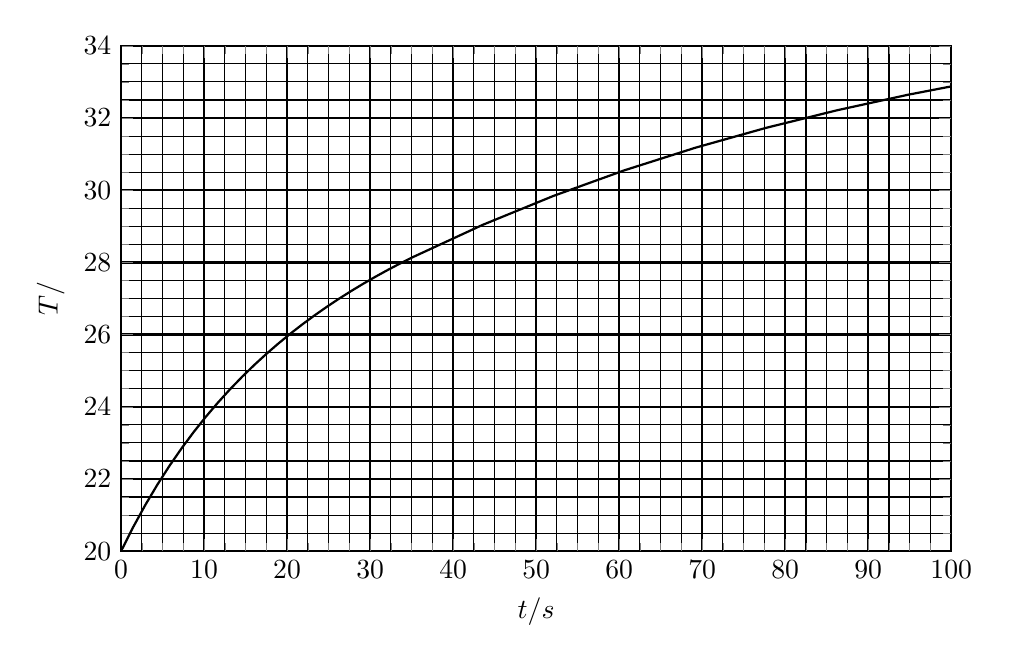
\begin{tikzpicture}
	\begin{axis}[ 
		xlabel={$t/s$},
		width = \textwidth,
		height = 8 cm,
		ylabel={$T/\si{\degreeCelsius}$},
		xmin=0, xmax = 100,
		ymin=20, ymax = 34,
		xtick distance = 10,
		ytick distance = 2,
		minor x tick num = 3,
		minor y tick num = 3,
		grid = both,
		minor grid style = {black},
		major grid style = {black, thick},
	] 
	\addplot [domain=0:35, thick]{20 + 2000/(4200*0.03)*(1-1/(1+0.03*x))};
	\addplot [domain=35:240, thick]
	{2000/(4200*0.03)+20+(20+ 2000/(4200*0.03)*(1-1/(1+0.03*35))
		-2000/(4200*0.03)-20)*e^(-0.03*(x-35)/(1+0.03*35))};
	\end{axis}
\end{tikzpicture}
\probend
\bigskip

% Ü175
\setAuthor{Ardi Loot}
\setRound{lõppvoor}
\setYear{2018}
\setNumber{G 5}
\setDifficulty{7}
\setTopic{Termodünaamika}

\prob{Soojustus}
\begin{wrapfigure}[10]{r}{0.5\textwidth}
\vspace{-30pt}
\begin{center}
\includegraphics[width=0.5\textwidth]{2018-v3g-05-kullastunud-aur}
\par\end{center} 
\end{wrapfigure}

Seina soojustus koosneb sisemisest (soojusjuhtivus $k_{1}=\SI{0.07}{W/\left(m\cdot K\right)}$)
ja välimisest kihist (soojusjuhtivus $k_{2}=\SI{0.05}{W/\left(m\cdot K\right)}$).
Nende kihtide vahel on kile, et takistada õhu liikumist läbi seina.
Millist tingimust peab rahuldama sisemise soojustuskihi pakus $L_{1},$
et vältida veeauru kondenseerumist seinas? Seina paksus $L=L_{1}+L_{2}=\SI{30}{cm},$
$L_{2}$ on välimise soojustuskihi paksus, toa temperatuur $T_{1}=\SI{20}{\degreeCelsius},$
suhteline õhuniiskus toas $\eta_{1}=\SI{60}{\percent}$ ja välistemperatuur
$T_{2}=\SI{-20}{\degreeCelsius}.$ Küllastunud veeauru osarõhu sõltuvus
temperatuurist on toodud joonisel.

\emph{Märkus.} Eeldada, et temperatuur muutub soojustuskihis lineaarselt
kaugusega ja muutuse kiirus on pöördvõrdeline soojusjuhtivusega.
\probend
\bigskip

% Ü176
\setAuthor{Stanislav Zavjalov}
\setRound{lõppvoor}
\setYear{2012}
\setNumber{G 7}
\setDifficulty{8}
\setTopic{Termodünaamika}

\prob{Ahi}
\begin{wrapfigure}{r}{0.5\textwidth}%
\includegraphics[width=\linewidth]{2012-v3g-07-ahi_graafik}%
\end{wrapfigure}
Väikese metallisulatusahju kütteelemendi võimsus on $P_0 = \SI{50}{W}$.
Toatemperatuuril olev ahi lülitakse sisse ja umbes 12 minuti pärast,
kui selle temperatuur praktiliselt enam ei kasva, pannakse ahju mitu
eelsoojendatud pliitükikest summaarse massiga $m = \SI{265}{g}$. Juuresoleval graafikul (suuremalt
lisalehel) on toodud
ahju temperatuuri sõltuvus ajast. Leidke selle põhjal plii sulamissoojus
$\lambda$.
\probend
\bigskip

% Ü177
\setAuthor{Ardi Loot}
\setRound{piirkonnavoor}
\setYear{2017}
\setNumber{G 10}
\setDifficulty{8}
\setTopic{Termodünaamika}

\prob{Gaasiküte}
Poolsfäärikujulist telki raadiusega $R=\SI{4}{m}$ köetakse
gaasipuhuriga. Seinte soojusjuhtivus on $U=\SI{3}{W/(m^{2}\cdot K)}$.
Ühe massiühiku gaasi põletamisel eraldub $D=\SI{2.25}{}$ massiühikut vett. Gaasi kütteväärtus on $k=\SI{40}{MJ/kg}$. Välisõhu temperatuur on $T_{0}=\SI{-10}{\degreeCelsius}$
ja õhuniiskus $\eta_{0}=\SI{50}{\percent}.$ Kui suur peab olema gaasikütte
võimsus $P$ ja telgi ventileerimise õhuruumala $Q$ ajaühikus, et hoida telgis
temperatuuri $T_{1}=\SI{15}{\degreeCelsius}$ ja õhuniiskust $\eta_{1}=\SI{80}{\percent}$?
Kui suur osa küttevõimusest kulub ventileeritava õhu soojendamiseks
ja mitu korda tunnis vahetub telgi õhk?

Õhu tihedus $\rho_{\tilde{o}}=\SI{1.2}{kg/m^{3}}$ ja soojusmahtuvus
$c_{\tilde{o}}=\SI{1.0}{kJ/(kg\cdot K)}$. Temperatuuril
$T_{0}=\SI{-10}{\degreeCelsius}$ mahub õhu ruumalaühikusse maksimaalselt
$G_{0}=\SI{2.3}{g/m^{3}}$ veeauru ning temperatuuril $T_{1}=\SI{15}{\degreeCelsius}$
vastavalt $G_{1}=\SI{12.8}{g/m^{3}}.$ Eeldada, et soojakaod läbi
telgi põranda puuduvad.
\probend
\bigskip

% Ü178
\setAuthor{Mihkel Pajusalu}
\setRound{lahtine}
\setYear{2014}
\setNumber{G 9}
\setDifficulty{9}
\setTopic{Termodünaamika}

\prob{Must kuup}
Olgu väga hea soojusjuhtivusega materjalist absoluutselt must kuup paralleelses valgusvihus, mille intensiivsus (võimsus ristlõikepindala kohta) on $I$. Milline on maksimaalne ja minimaalne stabiilne temperatuur $T_\text{max}$ ja $T_\text{min}$, mille kuup saavutab sõltuvalt selle asendist kiirguse leviku suuna suhtes?
\probend
\bigskip
\newpage\subsection{\protect\StrSubstitute{Varia}{-}{ }}

% Ü179
\setAuthor{EFO žürii}
\setRound{piirkonnavoor}
\setYear{2018}
\setNumber{G 1}
\setDifficulty{1}
\setTopic{Varia}

\prob{Kontraktsioon}
Omavahel segatakse $V_v$ liitrit vett ja $V_p$ liitrit piiritust nii, et tekkinud lahuse ruumala $V=\SI{1}{dm^3}$ ning lahuses on massi järgi $p=\SI{44,1}{\percent}$ piiritust. Leidke omavahel segatud vee ja piirituse ruumalad $V_v$ ja $V_p$. Lahuste kokkuvalamisel esineb $\gamma = \SI{6}{\percent}$-line kontraktsioon -- saadud lahuse ruumala on \SI{6}{\percent} väiksem kui vee ja piirituse ruumalade summa. Vee tihedus $\rho_v=\SI{1000}{kg/m^3}$ ning piirituse tihedus $\rho_p=\SI{790}{kg/m^3}$.
\probend
\bigskip

% Ü180
\setAuthor{Mihkel Kree}
\setRound{piirkonnavoor}
\setYear{2014}
\setNumber{G 4}
\setDifficulty{3}
\setTopic{Varia}

\prob{Mobiililaadija}
Leiutajad on pakkunud välja toreda seadme matkainimestele oma telefoni laadimiseks. Ühe saapa talla sisse pannakse mehhanism, mis toimib amortisaatorina. Iga kord kui kannale toetutakse, muundatakse mehaaniline töö väikese elektrigeneraatori abil elektrienergiaks. Oletame, et matkaja mass $m=\SI{60}{kg}$ ja ühe sammu ajal vajub tald kokku 
$h=\SI{5}{mm}$ võrra. Antud seadme kasutegur $\eta = \SI{0,2}{}$. Matkaja keskmiseks sammupaari pikkuseks ehk kahe järjestikuse samale kannale astumise vahemaaks võtame $d=\SI{1.5}{m}$. Nüüd tuleb vaid ühendada telefon juhtmega saapa külge ja aku laadimine võib alata.

Arvestage, et tüüpilises nutitelefonis on liitium-polümeeraku, mis töötab pingel $U=\SI{3.7}{V}$. Samuti arvestage, et kui telefon töötaks keskmisel voolutugevusel $I_k=\SI{130}{mA}$, suudaks aku vastu pidada $T=10$ tundi. Arvutage, kui pika maa peab matkaja maha kõndima, et tühi telefoni aku uuesti täis laadida.
\probend
\bigskip

% Ü181
\setAuthor{Valter Kiisk}
\setRound{lõppvoor}
\setYear{2017}
\setNumber{G 3}
\setDifficulty{3}
\setTopic{Varia}

\prob{Laser}
Laserkiir ühtlase diameetriga $d=\SI{1}{mm}$ langeb risti kiilukujulise klaasplaadi esimesele pinnale (pindade vaheline nurk $\varphi=\ang{2}$). Laserkiire koosseisus on monokromaatsed komponendid lainepikkustega $\lambda_1=\SI{355}{nm}$ ja $\lambda_2=\SI{532}{nm}$. Klaasi murdumisnäitajad nendel lainepikkustel on vastavalt $n_1=\num{1.48}$ ja $n_2=\num{1.46}$. Leidke kaugus $l$ klaasplaadist, kus erineva lainepikkusega valguskiired on teineteisest täielikult eraldunud.
\probend
\bigskip

% Ü182
\setAuthor{Koit Timpmann}
\setRound{lahtine}
\setYear{2011}
\setNumber{G 2}
\setDifficulty{4}
\setTopic{Varia}

\prob{Pindpinevus}
Klaastoru (raadius $r_1$) asetatakse jämedama klaastoru sisse nii, et nende teljed ühtivad. Seejärel
pannakse mõlemad püsti vette. Leidke, kui suur peaks olema jämedama toru
siseraadius $r_2$, et veetase oleks mõlemas klaastorus sama. Eeldage, et torude
seinad on tühiselt õhukesed.
\probend
\bigskip

% Ü183
\setAuthor{Ants Remm}
\setRound{lahtine}
\setYear{2011}
\setNumber{G 4}
\setDifficulty{4}
\setTopic{Varia}

\prob{Smurf solaariumis}
Smurf veetis solaariumi lampide all ajavahemiku $t = \SI{10}{min} $. Kui suure soojushulga $ Q $
sai Smurf? Joonistel on toodud Smurfile langenud valguse spekter $I$
(intensiivsus lainepikkuse kohta sõltuvalt valguse lainepikkusest, ühik
\SI{e9}{W/m^3}) ning Smurfi	
neeldumisspekter $\varepsilon$ (neelatud ja peale langenud valguse
intensiivsuste suhte
sõltuvus valguse lainepikkusest).
Smurfi efektiivne pindala, kuhu langeb valgus, on $ S = \SI{0,1}{m^2} $.
\begin{center}
\includegraphics[width=0.49\textwidth]{2011-lahg-04-I}
\includegraphics[width=0.49\textwidth]{2011-lahg-04-epsilon}
\end{center}
\probend
\bigskip

% Ü184
\setAuthor{Valter Kiisk}
\setRound{piirkonnavoor}
\setYear{2016}
\setNumber{G 7}
\setDifficulty{4}
\setTopic{Varia}

\prob{Valgustid}
Luminestsentstorust kaugusel $l_1=\SI{15}{cm}$ mõõdeti valgustatuseks $L_1=\SI{8400}{lx}$. Luminestsentstoru võib lugeda hulga pikemaks kaugusest $l_1$. Seevastu üksikust LED-pirnist kaugusel $l_2=\SI{30}{cm}$ mõõdeti valgustatuseks $L_2=\SI{2600}{lx}$. Kontoriruumis kulgevad luminestsentstorud ühe sirge katkematu rivina üle kogu ruumi, paiknedes töötasapinnast kõrgusel $h_1=\SI{1.8}{m}$. Laualambi LED-pirn paikneb kõrgusel $h_2=\SI{40}{cm}$ laua pinnast. Kui suur valgustatus saavutatakse otse valgusti all eraldi üldvalgustuse ja kohtvalgustuse kasutamisel? 

\emph{Märkus.} valgustatus iseloomustab ajaühikus pinnaühikule langevat valgusenergiat.
\probend
\bigskip

% Ü185
\setAuthor{Taavi Pungas}
\setRound{lõppvoor}
\setYear{2013}
\setNumber{G 6}
\setDifficulty{5}
\setTopic{Varia}

\prob{Tiik}
\begin{wrapfigure}{r}{0.25\textwidth}%
\includegraphics[width=\linewidth]{2013-v3g-06-lained}%
\end{wrapfigure}
Vaatleme tiiki visatud kivi ümber tekkinud lainetust. Kui kivi kukub vette,
tekib suur hulk erinevate lainepikkustega häiritusi, millest igaüks levib
omaette kiirusega. Nende liitumisel moodustub lainehari, mille liikumist
saame vaadelda. Joonisele (suuremalt lisalehele) on iga kindla ajavahemiku järel kantud selle
laineharja asukoht, mõõtkavaks sirglõik pikkusega~$L$. Laineharja kiirus $v$
sõltub seda parasjagu moodustavate komponentide lainepikkustest $\lambda$ ja vee
sügavusest $h$. Kui kivi vettekukkumisest möödunud aeg $t$ on väike, siis
koosneb lainehari lainepikkustest $\lambda \ll h$ ning laineharja kiirus sõltub
ajast seose $v \approx \frac{gt}{\pi}$ järgi. Kaugemal, kus laineharja
moodustavad häiritused lainepikkusega $\lambda \gg h$, liigub see kiirusega $v
\approx \sqrt{hg}$. Hinnake sügavust $h$ eeldusel, et see oli terve tiigi
ulatuses sama. Vastus andke suhtena~$h/L$.
\probend
\bigskip

% Ü186
\setAuthor{Mihkel Kree}
\setRound{lõppvoor}
\setYear{2016}
\setNumber{G 5}
\setDifficulty{5}
\setTopic{Varia}

\prob{Radoon}
Graptoliitargilliit (tuntud ka diktüoneemakilda nime all) on Põhja-Eestis paljanduv setteline savikivim, mis sisaldab hulgaliselt haruldasi elemente, muu hulgas uraani. Üks tonn kivimit sisaldab \SI{300}{g} uraan-238 isotoopi. Uraani levinuima isotoobi, aatommassiga $238$, poolestusaeg $\tau\idx{U}=\SI{4.5}{}$ miljardit aastat ning selle lagunemisahela vaheetapiks on radioaktiivne element radoon, aatommassiga $222$ ning poolestusajaga $\tau\idx{Rn}=\SI{3.8}{}$ päeva. Radoon on gaas, mida peetakse kopsuvähi tekitajaks, sest sissehingamisel satuvad organismi selle radioaktiivsed laguproduktid. Seetõttu sätestavad vastavad normatiivid, et hoonete ruumiõhus peab radooni aktiivsus olema väiksem kui \SI{200}{Bq/m^3}, kus	Henri Becquereli järgi nimetatud ühik \SI{}{Bq} tähistab üht tuuma lagunemist sekundis.

Matkaja tõi matkalt pahaaimamatult koju kaasa ühe graptoliitargilliidi tükikese massiga $m$ ning paigutas selle magamistuppa kapi peale. Arvestage lihtsustatult, et magamistoas ruumalaga $V=\SI{25}{m^3}$ õhuvahetust ei toimu ning et kogu tekkiv gaasiline radoon väljub kivimist. Leidke kivimitükikese suurim ohutu mass $m$, nii et sellest tingitud radooni aktiivsus jääks veel lubatud normidesse, kui kivimit hoida pikka aega toas. 

\emph{Märkus.} aatommassiühik $u=\SI{1.7e-27}{kg}$.
\probend
\bigskip

% Ü187
\setAuthor{Jaan Kalda}
\setRound{piirkonnavoor}
\setYear{2012}
\setNumber{G 7}
\setDifficulty{7}
\setTopic{Varia}

\prob{Vihmasadu}
Viilkatusega maja katus on peegelsümmeetriline: vertikaalne sümmeetriatasand on
ida-läänesuunaline ning katuse
põhja- ja lõunaküljed on omavahel risti. Mõlemal katusepoolel on vihmaveerenn,
mis kogub katusele langeva vee ning suunab selle tünni.
Sajab vihma ning puhub lõunatuul $u= \SI{6,0}{m/s}$; lõunaküljel paiknev tünn
täitub 2,0 korda kiiremini kui põhjaküljel paiknev tünn; võib
lugeda, et katuse läheduses piiskade langemissuund oluliselt ei muutu.
Milline on piiskade langemise keskmine kiirus (st kiiruse vertikaalkomponent)?
\probend
\bigskip

% Ü188
\setAuthor{Jaan Kalda}
\setRound{lõppvoor}
\setYear{2015}
\setNumber{G 6}
\setDifficulty{8}
\setTopic{Varia}

\prob{Lööklaine}
Elektrostaatilist lööklainet, mis levib kiirusega $w$ piki $x$-telge, võib kirjeldada elektrilise potentsiaali abil: $U=0$ kui $x<wt$ ning $U=U_0$ kui $x>wt$. Millise kiiruse $v$ omandab lööklaine mõjul algselt paigal seisnud osake massiga $m$ ning laenguga $q$? Vastus andke sõltuvana potentsiaalibarjääri kõrgusest $U_0$. Pöörake tähelepanu asjaolule, et see, kummale poole barjääri osake jääb, sõltub $U_0$ väärtusest.
\probend
\bigskip

% Ü189
\setAuthor{Jaan Kalda}
\setRound{lahtine}
\setYear{2013}
\setNumber{G 10}
\setDifficulty{10}
\setTopic{Varia}

\prob{Õhupalli vari}
Päikesepaistelisel päeval hõljub õhus kerakujuline läbipaistmatu õhupall, mis
jätab horisontaalsele maapinnale varju, kusjuures poolvarju pikkus on \SI{5,0}{m}
ja laius \SI{2,5}m ning täisvarju pikkus \SI{1,0}{m}. Kui suur on palli
läbimõõt ja kui kõrgel see on maapinnast? Päikese näiv nurkläbimõõt (see on nurk, 
mis moodustub kahe kiire vahel, mis on tõmmatud vaatleja silma juurest 
Päikese diameetri otspunktide juurde) oli sel
päeval $\alpha =0,53^\circ$.
\probend
\bigskip
\newpage\subsection{\protect\StrSubstitute{Vedelike mehaanika}{-}{ }}

% Ü190
\setAuthor{Koit Timpmann}
\setRound{piirkonnavoor}
\setYear{2012}
\setNumber{G 3}
\setDifficulty{2}
\setTopic{Vedelike mehaanika}

\prob{Tünn}
Vees ujuva tühja tünni ruumalast on $1/10$ vee sees. Pärast tünni täitmist
tundmatu vedelikuga jääb tünn vee peale ujuma, kuid nüüd on vee sees $9/10$ tünni
ruumalast. Kui suur on tünni valatud vedeliku tihedus? Vee tihedus on
\SI{1000}{kg/m^3}.
\probend
\bigskip

% Ü191
\setAuthor{Hans Daniel Kaimre}
\setRound{lõppvoor}
\setYear{2018}
\setNumber{G 2}
\setDifficulty{3}
\setTopic{Vedelike mehaanika}

\prob{Auk tünnis}
Suure vett täis tünni põhjas on auk, kust voolab vett välja. Graafikul on esitatud väljuva veejoa läbimõõdu sõltuvus kaugusest tünni põhjast $l$. Leidke veetaseme kõrgus tünnis.

\begin{center}
\includegraphics[width = 0.6\linewidth]{2018-v3g-02-juga.pdf}
\end{center}
\probend
\bigskip

% Ü192
\setAuthor{Koit Timpmann}
\setRound{lõppvoor}
\setYear{2015}
\setNumber{G 3}
\setDifficulty{4}
\setTopic{Vedelike mehaanika}

\prob{Ujuv kuup}
Õhukeseseinaline hermeetiline kuup ujub vee pinnal. Vee tihedus on $\rho$, kuubi mass koos selles oleva gaasiga $m$ ja selle serva pikkus $a$. Milline on vähim gaasi algrõhk kuubis $p$, mille korral kuup ei upuks, kui selle põhja tekiks auk? Õhurõhk on $p_0$, raskuskiirendus on $g$.
\probend
\bigskip

% Ü193
\setAuthor{Ardi Loot}
\setRound{piirkonnavoor}
\setYear{2018}
\setNumber{G 4}
\setDifficulty{4}
\setTopic{Vedelike mehaanika}

\prob{Pump}
Kaevust sügavusega $h=\SI{5.0}{m}$ tahetakse pumbata vett. Pump asub
maapinnal ning selle veevõtutoru (täidetud veega) on siseläbimõõduga
$d=\SI{16}{mm}$ ja pikkusega, mis on võrdne kaevu sügavusega.\\
\osa Kui suur peab olema pumba võimsus $P$, et pumbata vett vooluhulgaga
$q=\SI{30}{l/min}$? Pumba kasutegur on $\eta=\SI{25}{\percent}$.\\
\osa Missugune on maksimaalne kaevu sügavus $h_{m}$, mille korral on
võimalik sellist tüüpi pumbaga kaevust vett pumbata?

Arvestada, et torus olevale veesambale mõjub lisaks teistele jõududele
ka hõõrdejõud, mis põhjustab rõhu vähenemist toru pikkuse $l$ kohta $\Delta p=c_{h}q^{2}l/d^{5},$
kus $c_{h}=\SI{40}{Pa\cdot s^{2}/m^{2}}.$ Vee tihedus $\rho=\SI{1000}{kg/m^{3}}$,
raskuskiirendus $g=\SI{9.8}{m/s^{2}}$ ja õhurõhk $p_{0}=\SI{100}{kPa}.$
\probend
\bigskip

% Ü194
\setAuthor{Siim Ainsaar}
\setRound{piirkonnavoor}
\setYear{2013}
\setNumber{G 7}
\setDifficulty{5}
\setTopic{Vedelike mehaanika}

\prob{Veeklaas}
Silindrilisse klaasi, mille kõrgus on $H$ ja põhja raadius $r$, valati
vett kõrguseni $h$. Klaas kaeti paberilehega ja keerati
tagurpidi; paberi ja
klaasi vahelt voolas välja veekogus ruumalaga $V$. Kui paberit enam kinni ei
hoitud, jäi see sellegipoolest klaasi külge, ülejäänud vesi püsis klaasis.
Kui suur oli maksimaalselt paberi mass $m$? Õhurõhk oli $p_0$,
raskuskiirendus $g$ ning vee tihedus $\varrho$.
Kasutati kriitpaberit, mis vett ei imanud. Paberist lahtilaskmise hetkel olid 
õhu ja vee temperatuurid võrdsed.
\probend
\bigskip

% Ü195
\setAuthor{Erkki Tempel}
\setRound{lahtine}
\setYear{2014}
\setNumber{G 6}
\setDifficulty{5}
\setTopic{Vedelike mehaanika}

\prob{Klots vedelikes}
Silindrilises anumas põhja pindalaga $S$ on kaks mittesegunevat vedelikku tihedustega $\rho_1$ ja $\rho_2$. Anumasse asetatakse kuubikujuline klots ruumalaga $V$ ning tihedusega $\rho_k$ ($\rho_1>\rho_k>\rho_2$). Klots on täielikult vedelike sees ega puuduta anuma põhja.\\
\osa Kui suur osa klotsist asub alumises vedelikus?\\
\osa Kui palju muutub kahe vedeliku eralduspinna kõrgus pärast klotsi asetamist anumasse?
\probend
\bigskip

% Ü196
\setAuthor{Jonatan Kalmus}
\setRound{piirkonnavoor}
\setYear{2018}
\setNumber{G 7}
\setDifficulty{5}
\setTopic{Vedelike mehaanika}

\prob{Kuup veega}
Leidke veekoguse mass, mis tuleb valada kuupi, et see oleks võimalikult stabiilne, ehk süsteemi massikese oleks võimalikult madalal. Kuubi külje pikkus on $a$, mass $M$, vee tihedus $\rho$. Kuubi seina paksusega mitte arvestada. Kuup on täielikult sümmeetriline ehk sellel on olemas kõik 6 identset tahku.
\probend
\bigskip

% Ü197
\setAuthor{Mihkel Heidelberg}
\setRound{lahtine}
\setYear{2012}
\setNumber{G 5}
\setDifficulty{6}
\setTopic{Vedelike mehaanika}

\prob{Allveelaev}
\begin{wrapfigure}{r}{0.51\linewidth}%
\includegraphics[width=\linewidth]{2012-lahg-05-allveelaev_g}%
\end{wrapfigure}
Salaagent Bond põgeneb allveelaevalt selle torni kaudu. Tornis on algselt
rõhk sama mis õhurõhk vee peal: $p_0 = \SI{100}{kPa}$. Pärast torni ja ülejäänud
allveelaeva eraldava luugi sulgemist teeb ta seina sisse augu (vaata joonist), misjärel
täitub torn osaliselt veega. Seejärel avab Bond torni laeluugi ja ujub
koos vabaneva õhuga pinnale.\\
\osa Kui paks on õhukiht, mis jääb torni enne torni
laeluugi avamist ja pärast vee sissevoolamise lõppemist?\\
\osa Kui suur ja mis suunas (üles või alla) on õhu ja vee poolt laeluugile avaldatav summaarne jõud enne
avamist, kui veetase torni sees on jäänud paigale?
\par
Luugi pindala $S =
\SI{0,50}{m^2}$, veetase luugi kohal $h=\SI{25}{m}$, torni kõrgus 
$s=\SI{2,0}{m}$. Vee tihedus $\rho = \SI{1000}{kg/m^3}$, raskuskiirendus $g =
\SI{9,8}{m/s^2}$.
\probend
\bigskip

% Ü198
\setAuthor{Taavi Pungas}
\setRound{lahtine}
\setYear{2013}
\setNumber{G 7}
\setDifficulty{7}
\setTopic{Vedelike mehaanika}

\prob{Kauss}
Silindrikujuline metallkauss massiga $M=\SI{1}{kg}$ ja ruumalaga
$V_1=\SI{3}{dm^3}$ ujub vannis. Mari teeb eksperimenti ja valab ühtlaselt
$t=\SI{1}{s}$ jooksul kõrguselt $h=\SI{1,5}{m}$ kaussi kannutäie vett ruumalaga
$V_2=\SI{1,5}{dm^3}$. Ennustage eksperimendi tulemust: kas kauss läheb põhja või
ei? Põhjendage oma ennustust arvutustega. Vee tihedus $\rho=\SI{1000}{kg/m^3}$.
\probend
\bigskip

% Ü199
\setAuthor{Mihkel Kree}
\setRound{lahtine}
\setYear{2015}
\setNumber{G 7}
\setDifficulty{7}
\setTopic{Vedelike mehaanika}

\prob{Veejoad}
\begin{wrapfigure}{r}{0.2\textwidth}%
\vspace{-15pt}
\includegraphics[width=\linewidth]{2015-lahg-07-veejoadJoon}%
\end{wrapfigure}
Vertikaalse silindrilise anuma seina sisse on paljudele erinevatele kõrgustele tehtud pisikesed augud, millest voolab välja vett. Anumasse valatakse aeglaselt vett juurde nii, et veetase anumas püsib muutumatuna kõrgusel $H$. Leidke, millisesse ruumipiirkonda saab anumast väljuv vesi jõuda ehk avaldage veejugade mähispinna võrrand $xy$-teljestikus. Eeldage, et erinevad veejoad üksteist ei mõjuta.
\probend
\bigskip

% Ü200
\setAuthor{Erkki Tempel}
\setRound{piirkonnavoor}
\setYear{2016}
\setNumber{G 9}
\setDifficulty{7}
\setTopic{Vedelike mehaanika}

\prob{U-toru}
U-torusse ühtlase ristlõikepindalaga S on valatud vesi tihedusega $\rho_v$, nii et üle poole U-torust on veega täidetud ja kummagi täitmata osa pikkus on $h$. U-toru üks ots suletakse hermeetiliselt ning teise torusse valatakse aeglaselt õli kuni U-toru ülemise servani. Kui suur oli õli tihedus $\rho_{\text{õ}}$, kui on teada, et lisatud õlisamba kõrgus oli $l$? Atmosfäärirõhk on $p_0$.
\probend
\bigskip
\newpage\normalsize\section{Vihjed}
        \toggleHint
        
% V1
\setAuthor{Erkki Tempel}
\setRound{piirkonnavoor}
\setYear{2014}
\setNumber{G 1}
\setDifficulty{1}
\setTopic{Dünaamika}

\prob{Lendav pudel}
\hint
Nii pudelile kui veele mõjuvad täpselt samad jõud ning neid visatakse sama algkiirusega.
\probend
\bigskip

% V2
\setAuthor{Erkki Tempel}
\setRound{piirkonnavoor}
\setYear{2014}
\setNumber{G 2}
\setDifficulty{1}
\setTopic{Dünaamika}

\prob{Potsataja ja pähklid}
\hint
Antud olukorda on mugavam vaadelda rongiga kaasa liikuvas taustsüsteemis.
\probend
\bigskip

% V3
\setAuthor{Mihkel Rähn}
\setRound{lahtine}
\setYear{2016}
\setNumber{G 2}
\setDifficulty{1}
\setTopic{Dünaamika}

\prob{Kurv}
\hint
Autos istujad ei tunne külgsuunalist jõudu siis, kui summaarne jõud on tee pinnaga risti.
\probend
\bigskip

% V4
\setAuthor{Eero Vaher}
\setRound{lahtine}
\setYear{2012}
\setNumber{G 2}
\setDifficulty{2}
\setTopic{Dünaamika}

\prob{Kadunud rahakott}
\hint
Hoovõturaja alumises otsas on rahakott omandanud teatud horisontaalse kiiruse. Edasi hakkab rahakott liikuma mööda paraboolset trajektoori, kuni see taas vastu mäe nõlva kukub.
\probend
\bigskip

% V5
\setAuthor{Taavi Pungas}
\setRound{lahtine}
\setYear{2013}
\setNumber{G 1}
\setDifficulty{2}
\setTopic{Dünaamika}

\prob{Kivi}
\hint
Tikk hakkab poolkera pealt maha libisema siis, kui raskusjõu pinnaga paralleelne komponent ületab hõõrdejõu.
\probend
\bigskip

% V6
\setAuthor{Taavi Pungas}
\setRound{piirkonnavoor}
\setYear{2013}
\setNumber{G 4}
\setDifficulty{2}
\setTopic{Dünaamika}

\prob{Kelgutaja}
\hint
Fikseeritud $h$ ja $t$ puhul on nõlva kalle vähim siis, kui hõõrdejõud puudub.
\probend
\bigskip

% V7
\setAuthor{Taivo Pungas}
\setRound{lõppvoor}
\setYear{2013}
\setNumber{G 2}
\setDifficulty{2}
\setTopic{Dünaamika}

\prob{Pall}
\hint
Palli lennu kõrgus sõltub vastavale kõrgusele jõudmise aja ruudust.
\probend
\bigskip

% V8
\setAuthor{Mihkel Rähn}
\setRound{lahtine}
\setYear{2014}
\setNumber{G 1}
\setDifficulty{2}
\setTopic{Dünaamika}

\prob{Kaubarong}
\hint
\osa Horisontaalsel teel peab kaubarong ületama takistava hõõrdejõu.\\
\osa Lisaks hõõrdejõule peab rong nüüd ületama ka raskusjõu.
\probend
\bigskip

% V9
\setAuthor{Andreas Valdmann}
\setRound{lahtine}
\setYear{2014}
\setNumber{G 2}
\setDifficulty{2}
\setTopic{Dünaamika}

\prob{Vaakumkahur}
\hint
Pall jaotab kahuritoru kaheks kambriks. Pärast vasakpoolse membraani purustamist hakkab vasakpoolses kambris olev gaas palli paremale poole suruma.
\probend
\bigskip

% V10
\setAuthor{EFO žürii}
\setRound{lahtine}
\setYear{2016}
\setNumber{G 1}
\setDifficulty{2}
\setTopic{Dünaamika}

\prob{Mängukahur}
\hint
Kuna pall maandub kaldpinnale risti, siis liigub pall sellel hetkel nurgaga $\alpha$ vertikaali suhtes. Seega tulistatakse pall kahurist välja samuti nurga $\alpha$ all vertikaali suhtes ning pall põrkab kaldpinnalt tagasi sama nurga all.
\probend
\bigskip

% V11
\setAuthor{Oleg Košik}
\setRound{piirkonnavoor}
\setYear{2016}
\setNumber{G 2}
\setDifficulty{2}
\setTopic{Dünaamika}

\prob{Köievedu}
\hint
Vastavalt Newtoni III seadusele on nööri tõmme mõlema mehe jaoks sama suur, kuid vastupidises suunas. Lisaks nööri tõmbele mõjub kummalegi mehele vastassuunas hõõrdejõud.
\probend
\bigskip

% V12
\setAuthor{Moorits Mihkel Muru}
\setRound{lõppvoor}
\setYear{2017}
\setNumber{G 1}
\setDifficulty{2}
\setTopic{Dünaamika}

\prob{Vastlaliug}
\hint
Hõõrdejõu tõttu kulutatud energia sõltub läbitud teepikkusest ja selle kaldest, potentsiaalse energia vahe sõltub kõrguse muudust.
\probend
\bigskip

% V13
\setAuthor{Kaur Aare Saar}
\setRound{lahtine}
\setYear{2013}
\setNumber{G 3}
\setDifficulty{3}
\setTopic{Dünaamika}

\prob{Alpinist}
\hint
Jõudes kukkumise madalaimasse punkti, on alpinisti potentsiaalne energia läinud üle vedru potentsiaalseks energiaks. Pannes vastava seose kirja, on võimalik leida nööri pikenemise $x$.
\probend
\bigskip

% V14
\setAuthor{Taavi Pungas}
\setRound{piirkonnavoor}
\setYear{2014}
\setNumber{G 5}
\setDifficulty{3}
\setTopic{Dünaamika}

\prob{Langevarjuhüpe}
\hint
Nii Jukule kui ka Juhanile mõjub sama koefitsiendiga õhu hõõrdejõud, mis on raskusjõu poolt täielikult tasakaalustatud.
\probend
\bigskip

% V15
\setAuthor{Joonas Kalda}
\setRound{piirkonnavoor}
\setYear{2016}
\setNumber{G 4}
\setDifficulty{3}
\setTopic{Dünaamika}

\prob{Kelk}
\hint
Piirjuhul läheb kogu Juku potentsiaalne energia hõõrdejõu poolt eraldatud soojusenergiaks.
\probend
\bigskip

% V16
\setAuthor{Eero Vaher}
\setRound{lõppvoor}
\setYear{2016}
\setNumber{G 2}
\setDifficulty{3}
\setTopic{Dünaamika}

\prob{Pidurdus}
\hint
Auto kineetiline energia kulub pidurdusjõu ületamiseks ning potentsiaalse energia muuduks.
\probend
\bigskip

% V17
\setAuthor{Hans Daniel Kaimre}
\setRound{lõppvoor}
\setYear{2016}
\setNumber{G 3}
\setDifficulty{3}
\setTopic{Dünaamika}

\prob{Kahurikuul}
\hint
Selleks, et leida tegelikku kuuli kõrgust Maa pinnast, võib rakendada energia jäävuse seadust kuuli laskmise hetkel ja trajektoori kõrgeimas punktis.
\probend
\bigskip

% V18
\setAuthor{Andreas Valdmann}
\setRound{piirkonnavoor}
\setYear{2017}
\setNumber{G 3}
\setDifficulty{3}
\setTopic{Dünaamika}

\prob{Pendel}
\hint
Koormisele mõjuvad kolm jõudu: niidi pinge, raskuskiirendus ja kesktõmbekiirendus. Lisaks peab resultantjõud olema risti nööriga, sest vastasel juhul peaks koormise kiirenemisel nöör venima või lühenema.
\probend
\bigskip

% V19
\setAuthor{Jonatan Kalmus}
\setRound{lõppvoor}
\setYear{2017}
\setNumber{G 2}
\setDifficulty{3}
\setTopic{Dünaamika}

\prob{Mäenõlv}
\hint
Poole pedaalipöörde jooksul peab ratturi poolt tehtav töö kompenseerima ratta massikeskme tõusmisest kaasneva potentsiaalse energia muudu.
\probend
\bigskip

% V20
\setAuthor{Kristian Kuppart}
\setRound{lahtine}
\setYear{2011}
\setNumber{G 3}
\setDifficulty{4}
\setTopic{Dünaamika}

\prob{Veoauto}
\hint
Veepind võtab asendi, mis on risti sellele mõjuva resultantjõuga. Liikudes veoautoga seotud süsteemi, näeme, et resultantkiirendus on $\vec g - \vec a$.
\probend
\bigskip

% V21
\setAuthor{Andreas Valdmann}
\setRound{piirkonnavoor}
\setYear{2012}
\setNumber{G 5}
\setDifficulty{4}
\setTopic{Dünaamika}

\prob{Surmasõlm}
\hint
Autole mõjuvad raskusjõud ja tee toereaktsioon. Silmuses püsimiseks ei tohi toereaktsioon kaduda. Kriitiline olukord tekib silmuse ülemises punktis, sest siis on auto kiirus vähim ning raskusjõud tõmbab autot maksimaalselt teest eemale.
\probend
\bigskip

% V22
\setAuthor{Mihkel Kree}
\setRound{lõppvoor}
\setYear{2012}
\setNumber{G 2}
\setDifficulty{4}
\setTopic{Dünaamika}

\prob{Veejuga}
\hint
Torust väljuv vesi liigub nagu vabalt langev keha horisontaalsuunalise algkiirusega $v$. Seega on veejuga parabooli kujuga, mille parameetrid saab jooniselt mõõta.
\probend
\bigskip

% V23
\setAuthor{Aigar Vaigu}
\setRound{piirkonnavoor}
\setYear{2016}
\setNumber{G 6}
\setDifficulty{4}
\setTopic{Dünaamika}

\prob{Lasketiir}
\hint
Kuul liigub mööda paraboolselt trajektoori, kusjuures kiiruse horisontaalne komponent püsib konstantne, st $v_x = \const = v\cos\alpha$, ning vertikaalne komponent on ühtlaselt kiirenev $v_y = v\sin\alpha - gt$.
\probend
\bigskip

% V24
\setAuthor{Kaur Aare Saar}
\setRound{lõppvoor}
\setYear{2016}
\setNumber{G 4}
\setDifficulty{4}
\setTopic{Dünaamika}

\prob{Silinder}
\hint
Silindri impulsimoment ei muutu telje suhtes, mis läbib silindri ja pinna kontaktpunkte, sest hõõrdejõul puudub jõuõlg selle telje suhtes.
\probend
\bigskip

% V25
\setAuthor{Jonatan Kalmus}
\setRound{piirkonnavoor}
\setYear{2018}
\setNumber{G 5}
\setDifficulty{4}
\setTopic{Dünaamika}

\prob{Veok ringteel}
\hint
Liiga suure kiiruse korral hakkab veok tsentrifugaaljõu tõttu väliskurvis oleva serva suhtes ümber pöörama. Seega peab piirjuhul antud telje jaoks kehtima jõumomentide tasakaal.
\probend
\bigskip

% V26
\setAuthor{Ants Remm}
\setRound{lahtine}
\setYear{2012}
\setNumber{G 6}
\setDifficulty{5}
\setTopic{Dünaamika}

\prob{Kloori molekul}
\hint
Jagunemise käigus peab säilima summaarne impulss ning energia. Osakeste kiirusi on mugavam vaadelda komponentide kaupa. Selleks võib võtta, et $x$-telg on molekuli esialgse suunaga paralleelne ning $y$-telg sellega risti.
\probend
\bigskip

% V27
\setAuthor{Andres Põldaru}
\setRound{lahtine}
\setYear{2014}
\setNumber{G 5}
\setDifficulty{5}
\setTopic{Dünaamika}

\prob{Kiik}
\hint
Kokkupõrke käigus kehtib mõlema massi jaoks kangireegel. Lisaks kehtib kokkupõrge seni, kuni massid pöörlevad ümber kiige sama nurkkiirusega.
\probend
\bigskip

% V28
\setAuthor{Jaan Toots}
\setRound{lahtine}
\setYear{2015}
\setNumber{G 6}
\setDifficulty{5}
\setTopic{Dünaamika}

\prob{Vesiniku ioniseerimine}
\hint
Vesiniku aatomi ioniseerimiseks peab elektroni kineetiline energia olema suurem kui $E_0$. Elektroni ja prootoni kokkupõrke käigus säilib nii summaarne kineetiline energia kui ka impulss.
\probend
\bigskip

% V29
\setAuthor{Kristian Kuppart}
\setRound{piirkonnavoor}
\setYear{2015}
\setNumber{G 5}
\setDifficulty{5}
\setTopic{Dünaamika}

\prob{Veetoru}
\hint
Toru lõpus järsult pöörav vesi surub toru teatud jõuga külgsuunas. Antud jõud on leitav, kui vaadelda ajaühikus väljuva veehulga impulsimuutu siseneva veega võrreldes.
\probend
\bigskip

% V30
\setAuthor{Mihkel Kree}
\setRound{piirkonnavoor}
\setYear{2015}
\setNumber{G 6}
\setDifficulty{5}
\setTopic{Dünaamika}

\prob{Põrge}
\hint
Kuna põrge on elastne, säilib põrke käigus kineetiline energia. Impulsi kohta sama aga ei saa öelda, sest põrke ajal mõjuvad kinnituspunktile jõud. Küll aga säilib süsteemis summaarne impulsimoment kinnituspunkti suhtes, sest põrke ajal on kinnituspunktile mõjuvate jõudude õlad nullid ning põrge toimub nii kiiresti, et raskusjõuga pole vaja arvestada.
\probend
\bigskip

% V31
\setAuthor{Ardi Loot}
\setRound{lahtine}
\setYear{2016}
\setNumber{G 6}
\setDifficulty{5}
\setTopic{Dünaamika}

\prob{Rattur}
\hint
Ratturile mõjuvad laskumisel kolm jõudu: mäest allaviiv raskusjõud, takistav hõõrdejõud ning tuuletakistus. Rattur on saavutanud lõppkiiruse, kui need jõud on tasakaalustunud.
\probend
\bigskip

% V32
\setAuthor{Rasmus Kisel}
\setRound{piirkonnavoor}
\setYear{2017}
\setNumber{G 7}
\setDifficulty{5}
\setTopic{Dünaamika}

\prob{Kaks kuuli ja vedru}
\hint
Vaatamata sellele, et tundmatu kuuli mass ja vedru jäikus pole teada, võib neid ikkagi tundmatutena kasutada ning loota, et need lõppvastuses välja taanduvad.
\probend
\bigskip

% V33
\setAuthor{Moorits Mihkel Muru}
\setRound{lõppvoor}
\setYear{2017}
\setNumber{G 5}
\setDifficulty{5}
\setTopic{Dünaamika}

\prob{Reisirong}
\hint
Reisijale mõjub kolm omavahel ristiolevat kiirendust: raskuskiirendus, kesktõmbekiirendus ja joonkiirendus.
\probend
\bigskip

% V34
\setAuthor{Hans Daniel Kaimre}
\setRound{lõppvoor}
\setYear{2018}
\setNumber{G 4}
\setDifficulty{5}
\setTopic{Dünaamika}

\prob{Kaheosaline pendel}
\hint
Niidis kaob tõmbejõud, kui raskusjõu niidisuunaline komponent saab võrdseks tsentrifugaaljõuga. Kuuli kiirus asendis 3 on leitav energia jäävuse seadusest.
\probend
\bigskip

% V35
\setAuthor{Hans Daniel Kaimre}
\setRound{piirkonnavoor}
\setYear{2016}
\setNumber{G 8}
\setDifficulty{6}
\setTopic{Dünaamika}

\prob{Veerev pall}
\hint
Märkame, et kuna hõõrdejõud puudub, ei mõju süsteemile summaarset jõudu. Seega jääb klotsi ja palli summaarne massikese paigale.
\probend
\bigskip

% V36
\setAuthor{Tanel Kiis}
\setRound{lahtine}
\setYear{2012}
\setNumber{G 7}
\setDifficulty{7}
\setTopic{Dünaamika}

\prob{Pidurdamine}
\hint
Kuna suur keha liigub kahe põrke vahel teatud vahemaa võrra allapoole, ei toimu kokkupõrked iga $t$ tagant vaid natukene tihedamalt. Selleks, et leida, missuguse impulsi kuulike suurele kehale üle kannab, tasub kokkupõrget vaadelda suure keha süsteemis. Eelduse $m\ll M$ kohaselt on kokkupõrge võrreldav seinaga kokku põrkamisega.
\probend
\bigskip

% V37
\setAuthor{Madis Ollikainen}
\setRound{piirkonnavoor}
\setYear{2012}
\setNumber{G 9}
\setDifficulty{7}
\setTopic{Dünaamika}

\prob{Robin Hood}
\hint
Noole algkiirus on leitav lähteandmetest. Edasi peab nool tabama punkti koordinaatidega $(\SI{200}{m};\SI{-0,7}{m})$ alguspunkti suhtes. Selle jaoks saab kirja panna liikumisvõrrandi nii $x$- kui ka $y$-koordinaadi jaoks.
\probend
\bigskip

% V38
\setAuthor{Mihkel Rähn}
\setRound{lõppvoor}
\setYear{2014}
\setNumber{G 7}
\setDifficulty{7}
\setTopic{Dünaamika}

\prob{Sportauto}
\hint
Olukorda on mugav vaadelda autoga kaasa kiirenevas taustsüsteemis. Sellisel juhul rakendub autole kuus jõudu ning peab kehtima jõudude ning jõumomentide tasakaal.
\probend
\bigskip

% V39
\setAuthor{Kaur Aare Saar}
\setRound{lahtine}
\setYear{2015}
\setNumber{G 8}
\setDifficulty{7}
\setTopic{Dünaamika}

\prob{Latt}
\hint
Latile mõjub igas punktis hõõrdejõud, mis on vastupidine selle punkti liikumissuunale. Kogu mingile osale mõjuv hõõrdejõud on seega võrdeline selle osa pikkusega. Lisaks on teada, et hõõrdejõud üritavad takistada nii lati kulgliikumist kui ka selle pöörlemist.
\probend
\bigskip

% V40
\setAuthor{Tanel Kiis}
\setRound{piirkonnavoor}
\setYear{2013}
\setNumber{G 9}
\setDifficulty{8}
\setTopic{Dünaamika}

\prob{Õõnes kera}
\hint
Õõnsusega kera saab vaadelda positiivse tihedusega täidetud kera ja õõnsuse suuruse negatiivse tihedusega kera superpositsioonina. Sellisel juhul saab mugavalt kirja panna jõumomentide tasakaalu mõlema stsenaariumi jaoks.
\probend
\bigskip

% V41
\setAuthor{Andreas Valdmann}
\setRound{lõppvoor}
\setYear{2013}
\setNumber{G 9}
\setDifficulty{8}
\setTopic{Dünaamika}

\prob{Jalgpallurid}
\hint
Lihtsuse huvides tasub pallide kiirusi komponentide järgi vaadelda. Vertikaalne komponent $v_z$, horisontaalkomponent pikki jalgpallureid ühendavat sirget $v_y$ ning risti selle sirgega $v_x$. Kokkupõrke hetkel peab risti jalgpallureid ühendava sirgega läbitud vahemaa mõlemal pallil sama olema.
\probend
\bigskip

% V42
\setAuthor{Andres Põldaru}
\setRound{lahtine}
\setYear{2015}
\setNumber{G 9}
\setDifficulty{8}
\setTopic{Dünaamika}

\prob{Mutrivõti}
\hint
Esimesena on vaja leida, missugune on keermete pinnanormaali ja pöörlemistelje vaheline nurk $\alpha$. Selleks on mugav vaadelda mutrivõtme pinna jaotust. Selleks, et mutreid saaks kõvasti kinni keerata, peab hõõrdejõud tasakaalustama keermete suunas mõjuva jõu komponendi.
\probend
\bigskip

% V43
\setAuthor{Taavet Kalda}
\setRound{lahtine}
\setYear{2017}
\setNumber{G 8}
\setDifficulty{8}
\setTopic{Dünaamika}

\prob{Plokid}
\hint
Paneme tähele, et niidi pinge alumises nööris on kaks korda väiksem kui ülemises nööris. Selles saab veenduda, kui vaadelda alumisele plokile mõjuvaid jõudusid. Lisaks saab mõlema nööri jaoks kirja panna nende venimatuse tingimuse.
\probend
\bigskip

% V44
\setAuthor{Jaan Kalda}
\setRound{lahtine}
\setYear{2017}
\setNumber{G 9}
\setDifficulty{8}
\setTopic{Dünaamika}

\prob{Mänguauto}
\hint
Auto taustsüsteemis mõjub auto massikeskmele jõud $Ma$, kus $a$ on auto kiirendus. Lisaks mõjub tagaratastele hõõrdejõud ning mõlemale rattale toereaktsioon. Ülesande eelduste kohaselt peab mõlema poolperioodi jooksul kehtima jõudude ja jõumomentide tasakaal.
\probend
\bigskip

% V45
\setAuthor{Jaan Kalda}
\setRound{lahtine}
\setYear{2012}
\setNumber{G 10}
\setDifficulty{9}
\setTopic{Dünaamika}

\prob{Killud}
\hint
Kildude koguimpulss on null, seega moodustavad impulsivektorid kolmnurga, mille sarnasustegurid on võimalik kildude liikumissuundadest taastada. Sarnaselt saab toimida kildude kineetilise energia ja libisemiskaugustega.
\probend
\bigskip

% V46
\setAuthor{Roland Matt}
\setRound{lõppvoor}
\setYear{2012}
\setNumber{G 8}
\setDifficulty{9}
\setTopic{Dünaamika}

\prob{Liivakell}
\hint
Juhul, kui süsteemi massikeskme kõrgus on $x(t)$, siis Newtoni II seaduse kohaselt $M\ddot{x}(t) = F - Mg$, kus $M$ on süsteemi kogumass ja $F$ kaalu näit. Seega taandub ülesanne $x(t)$ leidmisele liivakella töörežiimis.
\probend
\bigskip

% V47
\setAuthor{Jaan Kalda}
\setRound{lõppvoor}
\setYear{2014}
\setNumber{G 8}
\setDifficulty{9}
\setTopic{Dünaamika}

\prob{Silindrilised anumad}
\hint
Üks võimalus sisemise silindri kiirenduse leidmiseks on rakendada virtuaalse nihke meetodit. Selle jaoks tuleb vaadelda, kuidas muutub süsteemi kineetiline ja potentsiaalne energia siis, kui sisemine silinder kerkib vahemaa $x$ võrra. Olles avaldanud süsteemi koguenergia $x$ kaudu, võib sellest tuletise võtta ning võrdsustada selle \num{0}-ga.
\probend
\bigskip

% V48
\setAuthor{Mihkel Kree}
\setRound{lõppvoor}
\setYear{2015}
\setNumber{G 8}
\setDifficulty{9}
\setTopic{Dünaamika}

\prob{Vedru}
\hint
Vastu maapinda kukkudes jääb kast hetkeliselt paigale ning koormis hakkab võnkuma ümber uue tasakaaluasendi ehk ümber punkti, kus vedru pinge tasakaalustab koormisele mõjuva raskusjõu. Järgneva liikumise käigus on kõige kriitilisem punkt see, kus koormis on kõige kõrgemas punktis. Sellisel juhul on kastile mõjuva vedru jõud maksimaalne.
\probend
\bigskip

% V49
\setAuthor{Jaan Kalda}
\setRound{lahtine}
\setYear{2017}
\setNumber{G 10}
\setDifficulty{9}
\setTopic{Dünaamika}

\prob{Vardad}
\hint
Punkti $B$ kiirust on võimalik leida, kasutades varraste venimatust ning asjaolu, et $A$ on fikseeritud. Punkti $B$ kiirenduse $AB$-sihilist komponenti saab leida kesktõmbekiirenduse kaudu ning kiirenduse suuna määramiseks on kasulik minna kiirusega $\vec{v}$ liikuvasse taustsüsteemi.
\probend
\bigskip

% V50
\setAuthor{Eero Vaher}
\setRound{piirkonnavoor}
\setYear{2016}
\setNumber{G 1}
\setDifficulty{1}
\setTopic{Elektriahelad}

\prob{Voltmeetrid}
\hint
Kuna voltmeetrit on ühesugused, võib need asendada takistustega $R$.
\probend
\bigskip

% V51
\setAuthor{Erkki Tempel}
\setRound{piirkonnavoor}
\setYear{2017}
\setNumber{G 1}
\setDifficulty{1}
\setTopic{Elektriahelad}

\prob{Voltmeeter}
\hint
Jooniselt näeme, et äärmised takistid on lühistatud, mistõttu need mõõteriistade näitu ei mõjuta.
\probend
\bigskip

% V52
\setAuthor{Mihkel Kree}
\setRound{piirkonnavoor}
\setYear{2015}
\setNumber{G 2}
\setDifficulty{2}
\setTopic{Elektriahelad}

\prob{Lambid}
\hint
Kuigi pingeallika pinge ja lampide takistused pole teada, võib neid kasutada muutujatena ja vaadata, kas need taanduvad lõppvastuses välja.
\probend
\bigskip

% V53
\setAuthor{Oleg Košik}
\setRound{piirkonnavoor}
\setYear{2013}
\setNumber{G 5}
\setDifficulty{3}
\setTopic{Elektriahelad}

\prob{Elektriskeem}
\hint
Mõlema kontuuri jaoks saab rakendada Ohmi seadust või Kirchhoffi seadusi.
\probend
\bigskip

% V54
\setAuthor{Eero Vaher}
\setRound{lahtine}
\setYear{2014}
\setNumber{G 4}
\setDifficulty{3}
\setTopic{Elektriahelad}

\prob{Tetraeeder}
\hint
Takistuse leidmiseks tasub tetraeedri pinna jaotus joonistada ning ära kasutada sümmeetriat.
\probend
\bigskip

% V55
\setAuthor{Taavi Pungas}
\setRound{lõppvoor}
\setYear{2014}
\setNumber{G 1}
\setDifficulty{3}
\setTopic{Elektriahelad}

\prob{Ruudustik}
\hint
Sümmeetria kaalutlustel saab skeemis sama potentsiaaliga punkte kokku ühendada.
\probend
\bigskip

% V56
\setAuthor{Hans Daniel Kaimre}
\setRound{lahtine}
\setYear{2015}
\setNumber{G 2}
\setDifficulty{3}
\setTopic{Elektriahelad}

\prob{Takistid}
\hint
Kogutakistuse määramist lihtsustab skeemi kavalam ümber joonistamine.
\probend
\bigskip

% V57
\setAuthor{Kristian Kuppart}
\setRound{lahtine}
\setYear{2016}
\setNumber{G 3}
\setDifficulty{3}
\setTopic{Elektriahelad}

\prob{Elektriskeem}
\hint
Kuna kondensaatorid on enne lüliti sulgemist laadimata, on ka pinge nende klemmidel $0$.\\
Pärast pika aja möödumist on kondensaatorite laeng jõudnud stabiliseerida ehk vool läbi kondensaatorite on $0$. Teisisõnu võib kondensaatorid efektiivselt skeemist lahti ühendada.
\probend
\bigskip

% V58
\setAuthor{Kristian Kuppart}
\setRound{lõppvoor}
\setYear{2013}
\setNumber{G 4}
\setDifficulty{4}
\setTopic{Elektriahelad}

\prob{Must kast}
\hint
Asjaolu, et voltmeeter näitab $\frac{U}{2}$, vihjab kondensaatorite jadaühendusele $C$ ja $D$ vahel.
\probend
\bigskip

% V59
\setAuthor{Sandra Schumann}
\setRound{lahtine}
\setYear{2017}
\setNumber{G 4}
\setDifficulty{4}
\setTopic{Elektriahelad}

\prob{Elektroonikaskeem}
\hint
Esimesel tekstis kirjeldatud juhul on kondensaatori pinge elektriskeemi sisselülitamise hetkel \SI{0}{V}, sest lüliti \enquote{väljasasendis} on takisti ja kondensaator jadamisi ühendatud. Teisel juhul on kondensaatori pinge koheselt pärast vooluallika polaarsuse muutmist \SI{9}{V}. Nende teadmistega saab leida takisti pinge mõlemal juhul ja kirja panna vastavad tingimused takisti läbipõlemise ja mitte läbipõlemise jaoks.
\probend
\bigskip

% V60
\setAuthor{Jaan Kalda}
\setRound{lõppvoor}
\setYear{2012}
\setNumber{G 3}
\setDifficulty{5}
\setTopic{Elektriahelad}

\prob{Elektriline sild}
\hint
Peegelsümmeetria tõttu ülemises ja alumises takistis ($R_2$ ja $R_4$) vool puudub.
\probend
\bigskip

% V61
\setAuthor{Jaan Kalda}
\setRound{lõppvoor}
\setYear{2015}
\setNumber{G 4}
\setDifficulty{5}
\setTopic{Elektriahelad}

\prob{Must kast}
\hint
Takistid saavad omavahel olla kas kolmnurk- või tähtühenduses. Ampermeeter ei saa olla otse väljundklemmide vahele lülitatud, sest siis põleks see vastavale klemmipaarile pinge rakendamisel läbi. Samuti ei saa see olla ühegi takistiga rööbiti lülitatud, sest siis ei läbiks vastavat takistit kunagi vool ning sisuliselt tähendaks see takisti asendamist null-takistusega.
\probend
\bigskip

% V62
\setAuthor{Jaan Kalda}
\setRound{lõppvoor}
\setYear{2017}
\setNumber{G 6}
\setDifficulty{5}
\setTopic{Elektriahelad}

\prob{Viisnurk}
\hint
Elektriskeemi käitumisest arusaamiseks tasub skeem selgemalt ümber joonistada, nii et ampermeeter on asendatud juhtmega ja voltmeeter lihtsalt kõrvaldatud.
\probend
\bigskip

% V63
\setAuthor{Valter Kiisk}
\setRound{piirkonnavoor}
\setYear{2018}
\setNumber{G 8}
\setDifficulty{5}
\setTopic{Elektriahelad}

\prob{12 lampi}
\hint
Eesmärk on leida elektriskeem, kus igale lambile langeb viiendik klemmipingest. Mõistlik on kõigepealt proovida võimalikult lihtsaid korrapäraseid lampide konfiguratsioone. Näiteks saab lambid asetada rööpühendusse, kus igas harus on kas 1, 2, 3, 4, 6 või 12 lampi.
\probend
\bigskip

% V64
\setAuthor{Eero Vaher}
\setRound{piirkonnavoor}
\setYear{2014}
\setNumber{G 8}
\setDifficulty{6}
\setTopic{Elektriahelad}

\prob{Elektriahela energia}
\hint
Kuna tegemist on jadaühendusega, siis on voolutugevus läbi kõikide vooluelementide sama. Lisaks peab pingelang üle kõikide vooluelementide olema \num{0}.
\probend
\bigskip

% V65
\setAuthor{Sandra Schumann}
\setRound{lõppvoor}
\setYear{2016}
\setNumber{G 7}
\setDifficulty{6}
\setTopic{Elektriahelad}

\prob{Vooluallikad}
\hint
Kuna elektriskeemis on mitu patareid ja vooluallikat, tuleb Kirchhoffi seadused ettevaatlikult iga kontuuri jaoks kirja panna. Juhul, kui lüliti on suletud, on vooluallikas efektiivselt lühistatud ning ülejäänud süsteemi järelikult ei mõjuta.
\probend
\bigskip

% V66
\setAuthor{Eero Vaher}
\setRound{lõppvoor}
\setYear{2018}
\setNumber{G 7}
\setDifficulty{6}
\setTopic{Elektriahelad}

\prob{Takistuste tuvastamine}
\hint
Takistuste leidmiseks tasub kõik \SI{1}{\ohm} takistuste kombinatsioonid läbi vaadata ning süstemaatiliselt valed konfiguratsioonid elimineerida.
\probend
\bigskip

% V67
\setAuthor{Mihkel Pajusalu}
\setRound{piirkonnavoor}
\setYear{2012}
\setNumber{G 8}
\setDifficulty{7}
\setTopic{Elektriahelad}

\prob{Raudtee}
\hint
Ülesandes peab käsitlema kahte juhtu: a) kui mõõtepunkt ei asu vaguni rataste vahel ja b) kui mõõtepunkt asub vaguni rataste vahel. Mõlemal juhul käitub tekkiv elektriskeem isemoodi.
\probend
\bigskip

% V68
\setAuthor{Mihkel Kree}
\setRound{lahtine}
\setYear{2013}
\setNumber{G 9}
\setDifficulty{7}
\setTopic{Elektriahelad}

\prob{Lambid}
\hint
Paneme tähele, et sümmeetria tõttu on lampide 1 ja 4 otspunktide potentsiaalid võrdsed.
\probend
\bigskip

% V69
\setAuthor{Jaan Kalda}
\setRound{lahtine}
\setYear{2012}
\setNumber{G 8}
\setDifficulty{8}
\setTopic{Elektriahelad}

\prob{Dioodid}
\hint
Oluline on tähele panna, et dioodidel saab pärivoolu korral pingeks olla ainult \SI{1,0}{V}. Tasub vaadata, kas rohkem kui ühel dioodil saab üldse vastava skeemi korral selline pinge olla.
\probend
\bigskip

% V70
\setAuthor{Jaan Kalda}
\setRound{lahtine}
\setYear{2016}
\setNumber{G 8}
\setDifficulty{8}
\setTopic{Elektriahelad}

\prob{Oktaeeder}
\hint
Et ampermeetrite sisetakistus on \num{0}, siis võime need lühistada: kõigis nendes tippudes, kuhu viivad ampermeetrid, on potentsiaalid võrdsed. Sümmeetria tõttu peab see 
potentsiaal jääma täpselt patareiklemmide potentsiaalide vahepeale, seega on igale takistile rakendatud pinge
$\SI 3V$.
\probend
\bigskip

% V71
\setAuthor{Jaan Kalda}
\setRound{lõppvoor}
\setYear{2018}
\setNumber{G 9}
\setDifficulty{8}
\setTopic{Elektriahelad}

\prob{Kondensaator}
\hint
Pärast lüliti avamist eraldub kogu energia kondensaatorilt lambis soojusena. Lisaks on kogu vabanev soojusenergia võrdne patarei kogutööga.
\probend
\bigskip

% V72
\setAuthor{Jaan Toots}
\setRound{lõppvoor}
\setYear{2015}
\setNumber{G 10}
\setDifficulty{10}
\setTopic{Elektriahelad}

\prob{Türistor}
\hint
Kirchhoffi esimese seaduse põhjal peab suvalise pinge ja voolutugevuse korral kehtima $V = U - IR$, kus $V$ on pinge türistoril. Kandes vastava funktsiooni volt-amperkarakteristikule on näha, et mingi pinge $U$ korral on $I$ ja $V$ jaoks kuni kolm lahendit, kusjuures negatiivse tõusuga punkt ei ole stabiilne, kuna vastaks negatiivsele takistusele. Antud informatsiooniga on võimalik määrata, kuidas türistorit läbiv vool muutub pingeallika pinge tõstmisel.
\probend
\bigskip

% V73
\setAuthor{Madis Ollikainen}
\setRound{lahtine}
\setYear{2012}
\setNumber{G 3}
\setDifficulty{2}
\setTopic{Elektrostaatika}

\prob{Kondensaator}
\hint
Kuulikesele mõjub nii raskusjõud kui ka elektrostaatiline jõud. Nende tulemusena hakkab kuul konstantse kiirendusega vertikaalselt üles liikuma.
\probend
\bigskip

% V74
\setAuthor{Mihkel Kree}
\setRound{lahtine}
\setYear{2017}
\setNumber{G 3}
\setDifficulty{4}
\setTopic{Elektrostaatika}

\prob{Elektron}
\hint
Plaatide vahel mõjub elektronile elektrivälja poolt allapoole suunatud kiirendus. Seega on elektroni kiirus plaatide vahelisest ruumist väljumisel minimaalne siis, kui elektroni trajektoor möödub alumise plaadi parema otsa lähedalt.
\probend
\bigskip

% V75
\setAuthor{Mihkel Kree}
\setRound{piirkonnavoor}
\setYear{2017}
\setNumber{G 9}
\setDifficulty{6}
\setTopic{Elektrostaatika}

\prob{Laengud}
\hint
Väikeste $y$-suunaliste võnkumiste jaoks on kasulik vaadata, missugune jõud kerale mõjub, kui seda väikse distantsi $y$ võrra tasakaaluasendist eemale nihutada.
\probend
\bigskip

% V76
\setAuthor{Jonatan Kalmus}
\setRound{lõppvoor}
\setYear{2018}
\setNumber{G 6}
\setDifficulty{7}
\setTopic{Elektrostaatika}

\prob{Pendel}
\hint
Elektrivälja lisamisel nihkub kuuli tasakaaluasend kas üles või alla, sõltuvalt elektrivälja suunast. Seega on igat poolperioodi mõistlik eraldi vaadata, sest selle raames liigub kuul ümber fikseeritud tasakaaluasendi.
\probend
\bigskip

% V77
\setAuthor{Stanislav Zavjalov}
\setRound{piirkonnavoor}
\setYear{2012}
\setNumber{G 10}
\setDifficulty{8}
\setTopic{Elektrostaatika}

\prob{Koonus}
\hint
Vastuse leidmiseks ei pea leidma täpset avaldist koonuse tipu potentsiaali jaoks, vaid piisab võrdelisuse seaduse leidmisest koonuse laengu ja lineaarmõõtme suhtes. Potentsiaalide jaoks kehtib ka superpositsiooniprintsiip ehk lõplik potentsiaal on esialgse koonuse potentsiaali ja äralõigatud koonuse potentsiaali vahe.
\probend
\bigskip

% V78
\setAuthor{Jaan Kalda}
\setRound{lõppvoor}
\setYear{2012}
\setNumber{G 9}
\setDifficulty{8}
\setTopic{Elektrostaatika}

\prob{Laengud}
\hint
Kuivõrd potentsiaal sõltub ainult $x$-koordinaadist, on elektriväli kõikjal $x$-telje sihiline ning
impulsi $y$-komponent säilib. Täielik \enquote{sisepeegeldus} toimub siis, kui positiivse $x-$suunaga 
seotud kineetiline energia on suurem kui $qU$.
\probend
\bigskip

% V79
\setAuthor{Stanislav Zavjalov}
\setRound{lõppvoor}
\setYear{2013}
\setNumber{G 10}
\setDifficulty{8}
\setTopic{Elektrostaatika}

\prob{Kondensaator}
\hint
Metallplaati sisse viies kondensaatori plaatide laeng säilib, aga pinge muutub. Kuna metallplaadi sees elektrivälja ei ole, on pingelang üle kondensaatori kaks korda väiksem, sest elektriväljaga täidetud piirkond väheneb $d/2$ võrra.
\probend
\bigskip

% V80
\setAuthor{Jaan Kalda}
\setRound{lahtine}
\setYear{2017}
\setNumber{G 7}
\setDifficulty{8}
\setTopic{Elektrostaatika}

\prob{Kondensaator}
\hint
Mahtuvuse leidmiseks võib kondensaatorit vaadelda kui kahte jadamisi ühendatud dielektrikuga kondensaatorit. Selleks asetame mõttelise metallplaadi dielektrilise kihi eralduspinnale. Eralduspinna laengu leidmiseks võib rakendada Gaussi teoreemi mõttelise \enquote{karbi} jaoks, mis hõlmab piirpinda.
\probend
\bigskip

% V81
\setAuthor{Jaan Kalda}
\setRound{piirkonnavoor}
\setYear{2015}
\setNumber{G 10}
\setDifficulty{9}
\setTopic{Elektrostaatika}

\prob{Laengutega pulk}
\hint
\osa Seni kuni üks laeng on piirkonnas $x>0$ ning teine piirkonnas $x<0$, on pulgale mõjuv summaarne jõud \num{0}; see tähendab, et pulk liigub konstantse kiirusega. Kui mõlemad laengud on piirkonnas $x>0$, mõjub pulgale elektrivälja poolt summaarne konstante jõud.\\
\osa Antud juhul sõltub pulgale mõjuv jõud lineaarselt pulga nihkest $x$.
\probend
\bigskip

% V82
\setAuthor{Jaan Kalda}
\setRound{lahtine}
\setYear{2016}
\setNumber{G 10}
\setDifficulty{9}
\setTopic{Elektrostaatika}

\prob{Kuulid}
\hint
Metallkeradele indutseeritakse elektrivälja poolt võrdsed ja vastasmärgilised laengud $\pm q$; kuivõrd traat on peenike,
siis võime ignoreerida sellel olevaid laenguid. Kuna metallkuulid käituvad nagu elektriline dipool, on süsteem tasakaalus siis, kui metalltraat on paralleelne elektriväljaga. Et traat on juhtivast materjalist, siis on süsteem ekvipotentsiaalne.
\probend
\bigskip

% V83
\setAuthor{Jaan Kalda}
\setRound{lõppvoor}
\setYear{2018}
\setNumber{G 10}
\setDifficulty{9}
\setTopic{Elektrostaatika}

\prob{Kaks kuuli}
\hint
Elektriväli indutseerib kuulidele vastasmärgilised laengud, mis tagavad, et kuulide potentsiaalid on võrdsed.
\probend
\bigskip

% V84
\setAuthor{Jaan Kalda}
\setRound{lõppvoor}
\setYear{2016}
\setNumber{G 10}
\setDifficulty{10}
\setTopic{Elektrostaatika}

\prob{Kolm kuuli}
\hint
\osa Kuulide ruutkeskmine kiirus on maksimaalne siis, kui elektriline potentsiaalne on minimaalne, st siis, kui nööride vahel on sirgnurk. Rakendades sümmeetriat ja impulsi ning energia jäävust, on võimalik antud olukorras kuulide kiirused leida.\\
\osa Paneme tähele, et $A$ kiireneb sümmeetria tõttu vertikaalselt. Peale kuulide vahelise tõukejõu tuleb arvestada ka niidi pingega.
\probend
\bigskip

% V85
\setAuthor{Eero Vaher}
\setRound{lõppvoor}
\setYear{2015}
\setNumber{G 1}
\setDifficulty{2}
\setTopic{Gaasid}

\prob{Õhupall}
\hint
Suurima võimaliku koormise massi korral on õhupalli keskmine tihedus võrdne õhu tihedusega.
\probend
\bigskip

% V86
\setAuthor{Eero Vaher}
\setRound{lahtine}
\setYear{2013}
\setNumber{G 4}
\setDifficulty{3}
\setTopic{Gaasid}

\prob{Õhupalli vägi}
\hint
Nii Maal kui ka Marsil peab õhupallile mõjuv üleslükkejõud kompenseerima koormise raskusjõu. Üleslükkejõud sõltub õhu tihedusest ning õhu tihedus on leitav ideaalse gaasi olekuvõrrandist.
\probend
\bigskip

% V87
\setAuthor{Mihkel Kree}
\setRound{lõppvoor}
\setYear{2014}
\setNumber{G 3}
\setDifficulty{4}
\setTopic{Gaasid}

\prob{Paisupaak}
\hint
Ideaalse gaasi olekuvõrrandiga on võimalik määrata, mis õhu ruumalaga avariiventiil avaneks. Õhu ruumala muudust on aga võimalik avaldada vajaliku vee tiheduse muudu.
\probend
\bigskip

% V88
\setAuthor{Kaur Aare Saar}
\setRound{lahtine}
\setYear{2015}
\setNumber{G 3}
\setDifficulty{4}
\setTopic{Gaasid}

\prob{Balloon}
\hint
Kuna balloon on silindrikujuline, on pinged selle telje sihis ning sellega ristuvas sihis erinevad. Mõlemal juhul peab ballooni seinas olev jõud tasakaalustama balloonisisese gaasi rõhu põhjustatud jõu.
\probend
\bigskip

% V89
\setAuthor{Mihkel Kree}
\setRound{piirkonnavoor}
\setYear{2016}
\setNumber{G 5}
\setDifficulty{4}
\setTopic{Gaasid}

\prob{Saunauks}
\hint
Kerisele visatud vee tekitatud lisarõhk on leitav ideaalse gaasi olekuvõrrandist. See rõhk mõjub ühtlaselt üle kogu ukse laiuse, seega tuleb uksele mõjuva jõumomendi arvutamisel võtta jõu õlaks pool ukse laiusest.
\probend
\bigskip

% V90
\setAuthor{Ardi Loot}
\setRound{lahtine}
\setYear{2017}
\setNumber{G 5}
\setDifficulty{4}
\setTopic{Gaasid}

\prob{Rattamatk}
\hint
On selge, et rehvi pumpamisel on rakendatav jõud võrdeline rehvis oleva rõhuga (õhurõhu suhtes). Rakendades jõudude tasakaalutingimust rehvi kokkupuutepinnale maaga, on võimalik leida kokkupuutepinna pindala, millest saab omakorda avaldada rehvi deformatsiooni ning rattarehvi ruumala muudu. Rattarehvi ruumala muudust tingitud rehvi siserõhu muutu on võimalik avaldada ideaalse gaasivõrrandiga.
\probend
\bigskip

% V91
\setAuthor{Rasmus Kisel}
\setRound{piirkonnavoor}
\setYear{2017}
\setNumber{G 6}
\setDifficulty{4}
\setTopic{Gaasid}

\prob{Silinder külmkapis}
\hint
Enne ja pärast jää sulamist saab kasutada ideaalse gaasi olekuvõrrandit. Lisaks saab aine massi jäävusest leida gaasi ruumalamuudu.
\probend
\bigskip

% V92
\setAuthor{Tundmatu autor}
\setRound{lahtine}
\setYear{2011}
\setNumber{G 5}
\setDifficulty{5}
\setTopic{Gaasid}

\prob{Süstal}
\hint
Kolvi lõppasendis tasakaalustab kolvile mõjuv hõõrdejõud rõhkude vahest tekitatud rõhumisjõu.
\probend
\bigskip

% V93
\setAuthor{Andreas Valdmann}
\setRound{piirkonnavoor}
\setYear{2012}
\setNumber{G 6}
\setDifficulty{5}
\setTopic{Gaasid}

\prob{Kuumaõhupall}
\hint
Õhupalli lendu tõusmise piiril peab kuumaõhupalli keskmine tihedus olema võrdne välisõhu tihedusega.
\probend
\bigskip

% V94
\setAuthor{Andreas Valdmann}
\setRound{lõppvoor}
\setYear{2012}
\setNumber{G 4}
\setDifficulty{5}
\setTopic{Gaasid}

\prob{Korvpall}
\hint
Sügavale vee alla sukeldamisel surub veesamba rõhk palli kokku. Pall hakkab ise põhja vajuma, kui tema ruumala väheneb nii palju, et pallile mõjuv üleslükkejõud saab väiksemaks raskusjõust ehk palli keskmine tihedus muutub väiksemaks vee tihedusest.
\probend
\bigskip

% V95
\setAuthor{Ardi Loot}
\setRound{lahtine}
\setYear{2016}
\setNumber{G 7}
\setDifficulty{6}
\setTopic{Gaasid}

\prob{Paisupaak}
\hint
Antud ülesandes on kolm tundmatut: paisupaagis oleva õhu moolide arv, paagi esialgne rõhk ning ruumala. Lisaks on tekstis kirjeldatud kolme tingimust, mida paak täitma peab; igaühe jaoks saab kirja panna ideaalse gaasi olekuvõrrandi.
\probend
\bigskip

% V96
\setAuthor{Valter Kiisk}
\setRound{piirkonnavoor}
\setYear{2017}
\setNumber{G 8}
\setDifficulty{7}
\setTopic{Gaasid}

\prob{Terasanum}
\hint
Anuma tugevuse määrab ilmselt seina paksus. Gaasi rõhust tingitud mehaaniline tõmbepinge anuma seintes ei tohi ületada väärtust $\sigma=\SI{450}{MPa}$. Tõmbepinge leidmiseks tasub anum mõtteliselt jaotada kahes poolsfääriks ning vaadelda neile mõjuvate jõudude tasakaalu.
\probend
\bigskip

% V97
\setAuthor{Ardi Loot}
\setRound{lõppvoor}
\setYear{2017}
\setNumber{G 7}
\setDifficulty{7}
\setTopic{Gaasid}

\prob{Õhupall}
\hint
Tasub vaadata, kuidas muutub õhupalli temperatuur, kui sinna teatud ruumala $V$ õhku sisse pumbata. Temperatuuri leidmiseks saab rakendada termodünaamika esimest seadust.
\probend
\bigskip

% V98
\setAuthor{Ants Remm}
\setRound{piirkonnavoor}
\setYear{2014}
\setNumber{G 10}
\setDifficulty{8}
\setTopic{Gaasid}

\prob{Kuumaõhupall}
\hint
Selleks, et kuumaõhupall õhuks püsiks, peab sees olev õhk olema piisavalt madala tihedusega, et üleslükkejõud tasakaalustaks kuumaõhupalli raskusjõu. Kui õhupalli sees on õhk temperatuuril $T$, siis õhupalli pooridest imbub välja soe õhk temperatuuril $T$, samas kui õhupalli siseneb õhk temperatuuril $T_0$. Propaani põletamine peab vastava soojuskao kompenseerima.
\probend
\bigskip

% V99
\setAuthor{Jaan Kalda}
\setRound{lõppvoor}
\setYear{2018}
\setNumber{G 8}
\setDifficulty{8}
\setTopic{Gaasid}

\prob{Kerkiv õhupall}
\hint
On võimalik näidata, et seni, kuni heelium pole võtnud enda alla veel kogu õhupalli ruumala, püsib tõstejõud konstante.
\probend
\bigskip

% V100
\setAuthor{Roland Matt}
\setRound{lahtine}
\setYear{2011}
\setNumber{G 1}
\setDifficulty{2}
\setTopic{Geomeetriline optika}

\prob{Segadus optikalaboris}
\hint
Selleks, et kiirtekimp laieneks ja jääks paralleelseks, pidi optik paigutama
nõgusläätse kumerläätse ette niimoodi, et läätsede fookused ühtiksid nõgusläätse
ees. Fookuste ühtimises saab veenduda, kasutades läätse valemit ning arvestades, et paralleelse kiirtekimbu kujutis asub lõpmatuses.
\probend
\bigskip

% V101
\setAuthor{Koit Timpmann}
\setRound{piirkonnavoor}
\setYear{2016}
\setNumber{G 3}
\setDifficulty{2}
\setTopic{Geomeetriline optika}

\prob{Lääts}
\hint
Pärast selge joonise joonestamist taandub ülesanne geomeetria peale.
\probend
\bigskip

% V102
\setAuthor{EFO žürii}
\setRound{lahtine}
\setYear{2017}
\setNumber{G 2}
\setDifficulty{2}
\setTopic{Geomeetriline optika}

\prob{Valgusallika kujutis}
\hint
$A$ asukoha leidmiseks võib kasutada läätsevalemit.
\probend
\bigskip

% V103
\setAuthor{Aigar Vaigu}
\setRound{piirkonnavoor}
\setYear{2017}
\setNumber{G 4}
\setDifficulty{2}
\setTopic{Geomeetriline optika}

\prob{Piiritusetehas}
\hint
Ainus muutus kiire teekonnas toimub segu sees. Murdumisnäitaja muutuse tõttu hakkab kiir segus teise nurga all liikuma. Vastavat nurga muutust ning seejärel ka $y$-suunalist nihet on võimalik leida Snelli seaduse abil.
\probend
\bigskip

% V104
\setAuthor{EFO žürii}
\setRound{piirkonnavoor}
\setYear{2018}
\setNumber{G 2}
\setDifficulty{2}
\setTopic{Geomeetriline optika}

\prob{Kaks valgusallikat}
\hint
Selleks, et kaks valgusallikat sama kujutise annaksid, peab üks olema näiline ja teine tegelik.
\probend
\bigskip

% V105
\setAuthor{Hans Daniel Kaimre}
\setRound{lõppvoor}
\setYear{2018}
\setNumber{G 1}
\setDifficulty{2}
\setTopic{Geomeetriline optika}

\prob{Poolitatud lääts}
\hint
Objekti kaugus läätsest on üheselt ära määratud sellega, et lääts on objektist ja kujutisest ühel kaugusel. Kiirte edasise käigu jaoks tuleb mõlemat läätse poolt eraldi vaadata.
\probend
\bigskip

% V106
\setAuthor{Taavi Pungas}
\setRound{lahtine}
\setYear{2012}
\setNumber{G 4}
\setDifficulty{3}
\setTopic{Geomeetriline optika}

\prob{Kärbes}
\hint
Kärbse kiiruse leidmiseks on kasulik vaadelda, kuidas kärbse poolt aja $t$ jooksul läbitud lõik pikkusega $vt$ läbi läätse välja venib.
\probend
\bigskip

% V107
\setAuthor{Oleg Košik}
\setRound{piirkonnavoor}
\setYear{2012}
\setNumber{G 1}
\setDifficulty{3}
\setTopic{Geomeetriline optika}

\prob{Peegel}
\hint
Tuttavad märkavad üksteist sellel hetkel, kui kiir, mis saab alguse ühest inimesest ning põrkab vastu peegli paremat nurka, jõuab teise inimeseni. Antud olukorra jaoks saab koostada joonise ning vastavad tingimused kirja panna.
\probend
\bigskip

% V108
\setAuthor{Tanel Kiis}
\setRound{lõppvoor}
\setYear{2013}
\setNumber{G 1}
\setDifficulty{3}
\setTopic{Geomeetriline optika}

\prob{Läätsed}
\hint
Ülesande lahendamiseks tasub vaadelda kõige äärmist kiirt, mis kumerläätse siseneb, ning abijoontega määratleda, kuidas vastav kiir optilist süsteemi läbib. Seejärel saab ära kasutada sarnaseid kolmnurki.
\probend
\bigskip

% V109
\setAuthor{Valter Kiisk}
\setRound{lõppvoor}
\setYear{2015}
\setNumber{G 2}
\setDifficulty{3}
\setTopic{Geomeetriline optika}

\prob{Valgustamine}
\hint
Antud juhul tasub vaadelda kõige äärmisi süsteemi sisenevaid kiiri.
\probend
\bigskip

% V110
\setAuthor{Andreas Valdmann}
\setRound{lahtine}
\setYear{2016}
\setNumber{G 4}
\setDifficulty{4}
\setTopic{Geomeetriline optika}

\prob{Optiline kiud}
\hint
Pikas optilises kius jäävad levima vaid sellised kiired, mille jaoks toimub südamiku ja katte lahutuspinnal täielik sisepeegeldumine.
\probend
\bigskip

% V111
\setAuthor{Andres Põldaru}
\setRound{lahtine}
\setYear{2016}
\setNumber{G 5}
\setDifficulty{4}
\setTopic{Geomeetriline optika}

\prob{Kolmlääts}
\hint
Pärast mõningast geomeetriat selgub, et $A$ on kahe vasakul oleva läätse fookuses; seega on punktist $A$ tulevad kiired pärast vastavate läätsede läbimist paralleelsed.
\probend
\bigskip

% V112
\setAuthor{Eero Vaher}
\setRound{piirkonnavoor}
\setYear{2017}
\setNumber{G 5}
\setDifficulty{4}
\setTopic{Geomeetriline optika}

\prob{Puuduv lääts}
\hint
Nõguslääts tekitab esemest näiva kujutise ning kumerlääts tekitab näivast kujutisest tõelise kujutise. Kuna kumerläätse asukoht on teada, saab tagurpidi lähenedes rekonstrueerida näilise kujutise asukoha.
\probend
\bigskip

% V113
\setAuthor{Andreas Valdmann}
\setRound{lõppvoor}
\setYear{2014}
\setNumber{G 4}
\setDifficulty{5}
\setTopic{Geomeetriline optika}

\prob{Periskoopprillid}
\hint
Nurga $\varphi$ leidmiseks tuleb vaadelda kiirt, mis siseneb lõiku $AB$.
\probend
\bigskip

% V114
\setAuthor{Mihkel Kree}
\setRound{lahtine}
\setYear{2015}
\setNumber{G 5}
\setDifficulty{5}
\setTopic{Geomeetriline optika}

\prob{Lääts}
\hint
Läätse asukoha leidmiseks tasub vaadata geomeetriliselt omapäraseid kiiri ja kuidas need läbi läätse murduvad. Selleks sobivad näiteks kiired AB, AA' ja BB'.
\probend
\bigskip

% V115
\setAuthor{Sandra Schumann}
\setRound{lõppvoor}
\setYear{2018}
\setNumber{G 3}
\setDifficulty{5}
\setTopic{Geomeetriline optika}

\prob{Peegelpõhi}
\hint
Paneme tähele, et valemi järgi keskkonna murdumisnäitaja suurenedes, kuid läätse murdumisnäitaja samaks jäädes läätse fookuskaugus suureneb. Seega on ainus viis, kuidas valguskiired saaksid ka pärast anuma vett täis valamist samas punktis koonduda, see, kui vees peegelduksid valguskiired põhjas olevalt peeglilt ja seejärel koonduksid samas punktis, kus enne.
\probend
\bigskip

% V116
\setAuthor{Eero Vaher}
\setRound{piirkonnavoor}
\setYear{2015}
\setNumber{G 8}
\setDifficulty{6}
\setTopic{Geomeetriline optika}

\prob{Fookuskaugus}
\hint
Läätse fookuskauguse leidmiseks tasub vaadelda valguskimpu, mille suund on paralleelne optilise peateljega. Sellisel juhul tekitavad kiired näilise kujutise läätse fookusesse.
\probend
\bigskip

% V117
\setAuthor{Jaan Kalda}
\setRound{lõppvoor}
\setYear{2012}
\setNumber{G 6}
\setDifficulty{7}
\setTopic{Geomeetriline optika}

\prob{Toru}
\hint
Kui peegeldavate silindriliste seinte asemel oleks kaks tasapeeglit, siis
tekiks optilise peateljega risti punktallika kujutiste lõpmatu jada (peegeldus, peegelduse peegeldus jne). Iga peegeldus tekitaks läbi läätse ekraanil uue kujutise. Tasapeeglite juhtu on võimalik ka silindrilise peegli peale laiendada.
\probend
\bigskip

% V118
\setAuthor{Valter Kiisk}
\setRound{lõppvoor}
\setYear{2013}
\setNumber{G 7}
\setDifficulty{7}
\setTopic{Geomeetriline optika}

\prob{Mikroskoop}
\hint
Mõlemad teravustatavuse asendid on üksteise suhtes sümmeetrilised. See tähendab seda, et kui esimeses asendis on läätse kaugus esemest $a$ ja sensorist $b$, siis teises asendis on vastavad kaugused ümber vahetatud.
\probend
\bigskip

% V119
\setAuthor{Erkki Tempel}
\setRound{lahtine}
\setYear{2014}
\setNumber{G 7}
\setDifficulty{7}
\setTopic{Geomeetriline optika}

\prob{Optiline skeem}
\hint
Algselt paralleelsed kiired koonduvad pärast läätse läbimist fokaaltasandis. Seega on võimalik esimese läätse fokaaltasand rekonstrueerida, teades fookuse asukohta ja kahe kiire lõikepunkti.
\probend
\bigskip

% V120
\setAuthor{Valter Kiisk}
\setRound{lõppvoor}
\setYear{2016}
\setNumber{G 6}
\setDifficulty{7}
\setTopic{Geomeetriline optika}

\prob{Luup}
\hint
Poolkera kumera pinna keskosa võib vaadelda omaette õhukese läätsena, mille fookuskaugus ja kaugus paberi pinnast määravad kujutise suurenduse. Läätse fookuskauguse leidmiseks on kasulik vaadelda valguskiirt, mis liigub paralleelselt optilise peateljega. Pärast läätses murdumist koondub kiir fookusesse.
\probend
\bigskip

% V121
\setAuthor{Andreas Valdmann}
\setRound{lõppvoor}
\setYear{2016}
\setNumber{G 8}
\setDifficulty{8}
\setTopic{Geomeetriline optika}

\prob{Nurgapeegel}
\hint
Juku näo kujutise leidmiseks tasub kõigepealt vaadelda, kuidas Juku silmad peeglites kujutisi tekitavad. Kuna peeglid on üksteise suhtes täisnurga all, on selge, et otse nurgapeegli nurka vaadates on näha kolmandat järku kujutis.
\probend
\bigskip

% V122
\setAuthor{Jaan Kalda}
\setRound{lõppvoor}
\setYear{2015}
\setNumber{G 7}
\setDifficulty{9}
\setTopic{Geomeetriline optika}

\prob{Ring ja ellips}
\hint
Esimesena tuleks alustada läätse keskpunkti leidmisega, seejärel paika panna läätse orientatsioon ning fookus. Keskpunkti leidmiseks tasub vaadata kiiri, mis puutuvad nii ringi kui ka ellipsit.
\probend
\bigskip

% V123
\setAuthor{Ardi Loot}
\setRound{lõppvoor}
\setYear{2017}
\setNumber{G 8}
\setDifficulty{9}
\setTopic{Geomeetriline optika}

\prob{Kaamera}
\hint
Tekitagu lõpmatuses asuv objekt läbi kumerläätse ja nõgusläätse vastavalt kujutised $A'$ ja $A$. Kaamera vaatenurk on leitav, vaadates olukorda, kus $A$ asub valgustundliku elemendi ääres. Sellisel juhul on kaamera vaatenurk $A'$ poolt kaetav nurk kumerläätse keskpunktist vaadatuna.
\probend
\bigskip

% V124
\setAuthor{Jaan Kalda}
\setRound{lõppvoor}
\setYear{2014}
\setNumber{G 10}
\setDifficulty{10}
\setTopic{Geomeetriline optika}

\prob{Klaassilinder}
\hint
Tähistame märgitud punkti $A$-ga ja silindri keskpunkti $O$-ga. Antud ülesande kontekstis tasub vaadelda funktsiooni $f(\alpha) = \delta$, mis kirjeldab punktist $A$ alguse saanud kiire silindrist väljumise nurka $\delta$ kiire $AO$ suhtes funktsioonina stardinurgast $\alpha$ kiire $AO$ suhtes. Silindri algasendit kirjeldab $f(\alpha) = 0$ kolme lahendiga. Lisaks on teada, et $f(\alpha) = \ang{15}$ on lahenditeta.
\probend
\bigskip

% V125
\setAuthor{Koit Timpmann}
\setRound{piirkonnavoor}
\setYear{2013}
\setNumber{G 1}
\setDifficulty{1}
\setTopic{Kinemaatika}

\prob{Rong}
\hint
Kiirendamise ning pidurdamise käigus on rongi keskmine kiirus $v\idx{max}/2$.
\probend
\bigskip

% V126
\setAuthor{Mihkel Kree}
\setRound{lahtine}
\setYear{2015}
\setNumber{G 1}
\setDifficulty{2}
\setTopic{Kinemaatika}

\prob{Rongivile}
\hint
Tasub vaadata, kuidas heli poolt läbitav vahemaa muutub vile laskmise alguses ja lõpus.
\probend
\bigskip

% V127
\setAuthor{Erkki Tempel}
\setRound{piirkonnavoor}
\setYear{2015}
\setNumber{G 1}
\setDifficulty{2}
\setTopic{Kinemaatika}

\prob{Kaubarong}
\hint
Peale teejupi, kus rong sõidab kiirusega \SI{18}{km/h}, tulevad rongil ajakaod ka teelõikudel, kus rong pidurdab ja kiireneb.
\probend
\bigskip

% V128
\setAuthor{Sandra Schumann}
\setRound{lahtine}
\setYear{2017}
\setNumber{G 1}
\setDifficulty{2}
\setTopic{Kinemaatika}

\prob{Kiirabiauto}
\hint
Nii kiirabiauto lähenemise kui ka kaugenemise jaoks saab kirja panna Doppleri seaduse. Lisaks on sageduste suhe üheselt määratud asjaoluga, et kiirabiauto sireeni toon langes väikese tertsi võrra.
\probend
\bigskip

% V129
\setAuthor{Mihkel Rähn}
\setRound{piirkonnavoor}
\setYear{2017}
\setNumber{G 2}
\setDifficulty{2}
\setTopic{Kinemaatika}

\prob{Pidurdus}
\hint
\osa Kõige suurem kokkupõrke oht on siis, kui esimene on jõudnud täielikult seiskuda (selles saab veenduda, kui liikuda tagumise autoga kaasa liikuvasse taustsüsteemi).\\
\osa Kahe liikuva objekti suhtelist liikumist on kasulik uurida liikuvas taustsüsteemis.
\probend
\bigskip

% V130
\setAuthor{Jaan Kalda}
\setRound{lõppvoor}
\setYear{2013}
\setNumber{G 3}
\setDifficulty{4}
\setTopic{Kinemaatika}

\prob{Jalgrattur}
\hint
Vaadeldes tuule ja jalgratturi kiirusi vektoritena, on võimalik geomeetriliselt konstrueerida vastavad tekstis toodud tingimused ning geomeetria põhjal tuule kiirus välja arvutada.
\probend
\bigskip

% V131
\setAuthor{Jaan Toots}
\setRound{lõppvoor}
\setYear{2014}
\setNumber{G 2}
\setDifficulty{4}
\setTopic{Kinemaatika}

\prob{Viiul}
\hint
Tekkival seisulainel peavad olema sõlmed mõlemas keele võnkuva osa otspunktis. Viiuli keelt puudutades peab ka keele puutepunkt sõlmpunkt olema.
\probend
\bigskip

% V132
\setAuthor{Taavi Pungas}
\setRound{piirkonnavoor}
\setYear{2012}
\setNumber{G 4}
\setDifficulty{5}
\setTopic{Kinemaatika}

\prob{Pöördlava}
\hint
Näitleja liikumist on mugav vaadelda kettaga seotud taustsüsteemis. Sellisel juhul pöörleb maapind nurkkiirusega $\frac{2\pi}{T}$ ning näitleja kõnnib ketta peal kiirusega $v$.
\probend
\bigskip

% V133
\setAuthor{Eero Vaher}
\setRound{lõppvoor}
\setYear{2015}
\setNumber{G 5}
\setDifficulty{5}
\setTopic{Kinemaatika}

\prob{Pallivise}
\hint
Palli lendu on mugav vaadelda laboratoorses taustsüsteemis. Sellisel juhul liigub pall pärast viset ühtlaselt ning sirgjooneliselt, kusjuures selle kiiruse vertikaalsihiline komponent on $v$ ning horisontaalsihiline komponent $\omega R$.
\probend
\bigskip

% V134
\setAuthor{Siim Ainsaar}
\setRound{lõppvoor}
\setYear{2012}
\setNumber{G 5}
\setDifficulty{6}
\setTopic{Kinemaatika}

\prob{Rehvid}
\hint
Selleks, et autorehvid kuluksid vähimal määral, peavad rattad pöörama ühtse kehana. Kuna rattad ei libise, asub pöörlemiskese rataste teljel.
\probend
\bigskip

% V135
\setAuthor{Jaan Kalda}
\setRound{lõppvoor}
\setYear{2014}
\setNumber{G 5}
\setDifficulty{6}
\setTopic{Kinemaatika}

\prob{Kammid}
\hint
Kui hall kamm liigub ühe pii võrra, on uus pilt identne esialgsega ning järelikult on tume laik liikunud ühe \enquote{lainepikkuse} võrra.
\probend
\bigskip

% V136
\setAuthor{Mihkel Kree}
\setRound{lahtine}
\setYear{2014}
\setNumber{G 10}
\setDifficulty{8}
\setTopic{Kinemaatika}

\prob{Päikese pöörlemine}
\hint
Mõõdetud lainepikkuste erinevus tuleneb mõõdetud punktide kiiruste vahest vaatleja suhtes. Kui Päikese pöörlemise nurkkiirus ekvaatoril on $v$, siis üks ekvaatori ots eemaldub vaatlejast kiirusega $v$ ja teine läheneb kiirusega $v$. Antud kiirusele vastav lainepikkuse muut on leitav Doppleri nihkest.
\probend
\bigskip

% V137
\setAuthor{Jaan Kalda}
\setRound{lõppvoor}
\setYear{2014}
\setNumber{G 9}
\setDifficulty{8}
\setTopic{Kinemaatika}

\prob{Traatrõngad}
\hint
Liikudes süsteemi, mis pöörleb nurkkiirusega $\omega/2$, on võimalik olukorra sümmeetriat ära kasutada.
\probend
\bigskip

% V138
\setAuthor{Jaan Kalda}
\setRound{lahtine}
\setYear{2016}
\setNumber{G 9}
\setDifficulty{9}
\setTopic{Kinemaatika}

\prob{Anemomeeter}
\hint
Leviaegade suhtelised erinevused on väikesed, seega võib lugeda, et helikiirus on hulga suurem tuule kiirusest. Heli levikut on kasulik vaadata tuulega seotud taustsüsteemis.
\probend
\bigskip

% V139
\setAuthor{Jaan Kalda}
\setRound{lõppvoor}
\setYear{2016}
\setNumber{G 9}
\setDifficulty{9}
\setTopic{Kinemaatika}

\prob{Kaater}
\hint
Ülesandes antud algandmed kirjeldavad kaatri liikumist tuule suhtes. Seega tasub olukorda vaadelda tuulega kaasa liikuvas taustsüsteemis.
\probend
\bigskip

% V140
\setAuthor{Kristian Kuppart}
\setRound{lahtine}
\setYear{2013}
\setNumber{G 2}
\setDifficulty{3}
\setTopic{Magnetism}

\prob{Magnetpeegel}
\hint
Magnetväljas hakkab osake liikuma mööda ringjoont, mille raadius on leitav jõudude tasakaalust. Maksimaalse nurga korral väljub osake magnetribast eraldusjoonega paralleelselt.
\probend
\bigskip

% V141
\setAuthor{Andreas Valdmann}
\setRound{lahtine}
\setYear{2013}
\setNumber{G 5}
\setDifficulty{4}
\setTopic{Magnetism}

\prob{Generaator}
\hint
Elektrivool generaatori mähises (juhtmekontuuris) tekib elektromagnetilise induktsiooni toimel ning seda protsessi kirjeldab Faraday seadus $\varepsilon = -\frac{\Delta\Phi}{\Delta t}$, kus $\varepsilon$ on voltides mõõdetav elektromotoorjõu suurus ning $\Delta\Phi$ on juhtmekontuuri läbiva magnetvoo muutus, mis toimub ajavahemiku $\Delta t$ jooksul.
\probend
\bigskip

% V142
\setAuthor{Eero Vaher}
\setRound{lahtine}
\setYear{2013}
\setNumber{G 6}
\setDifficulty{5}
\setTopic{Magnetism}

\prob{Tiirlev kuulike}
\hint
Magnetväljas ringliikumisel käitub Lorentzi jõud kesktõmbejõuna. Analoogselt on teisel juhul kesktõmbejõud kuloniline jõud kahe kuuli vahel, kusjuures peab tähelepanu pöörama sellele, et kuulid tiirlevad ümber ühise massikeskme.
\probend
\bigskip

% V143
\setAuthor{Kristian Kuppart}
\setRound{piirkonnavoor}
\setYear{2018}
\setNumber{G 10}
\setDifficulty{6}
\setTopic{Magnetism}

\prob{Tsüklotron}
\hint
Osakesed hakkavad tsüklotronis liikuma päripäeva mööda järjest suureneva raadiusega poolringjooni. Osake väljub tsüklotronist, kui tema trajektoori raadius kasvab sama suureks tsüklotroni raadiusega $R$.
\probend
\bigskip

% V144
\setAuthor{Kristian Kuppart}
\setRound{piirkonnavoor}
\setYear{2013}
\setNumber{G 10}
\setDifficulty{7}
\setTopic{Magnetism}

\prob{Mass-spektromeeter}
\hint
Osakeste kiirus magnetvälja sisenedes on avaldatav energia jäävusest. Magnetväljas algab ringliikumine, kusjuures detektorini jõutakse pärast poole ringjoone läbimist. Teisisõnu on detekteeritud $x$-koordinaat $2R$, kus $R$ on ringjoone raadius.
\probend
\bigskip

% V145
\setAuthor{Jaan Kalda}
\setRound{piirkonnavoor}
\setYear{2015}
\setNumber{G 9}
\setDifficulty{8}
\setTopic{Magnetism}

\prob{Magnetväli}
\hint
Laeng sooritab magnetväljas ringliikumist; mida suurem on magnetväli, seda suurem on ringi raadius. Enne ja pärast ringliikumist on osakese trajektoor sirge, kusjuures ülemine ringjooneks on ilma murdepunktita, st sirgjooned on ringjoone puutujaks.
\probend
\bigskip

% V146
\setAuthor{Eero Vaher}
\setRound{lahtine}
\setYear{2015}
\setNumber{G 10}
\setDifficulty{9}
\setTopic{Magnetism}

\prob{Laetud pendel}
\hint
Kuulikesele mõjuvad raskusjõud, niidi pinge ning Lorentzi jõud. Kuulike püsib ringjoone kaare kujulisel trajektooril seni, kuni Lorentzi jõud ja niidi pinge ületavad ülejäänud jõudude niidisihilise komponendi. Vastav kriitiline nurk on leitav energia jäävuse seadusest ning jõudude tasakaalust.
\probend
\bigskip

% V147
\setAuthor{Jaan Kalda}
\setRound{lõppvoor}
\setYear{2017}
\setNumber{G 10}
\setDifficulty{10}
\setTopic{Magnetism}

\prob{Elektronid}
\hint
Elektronid hakkavad liikuma mööda $z$-teljelist heeliksit, kusjuures heeliksi raadius on võrdeline $x-y$ suunalise kiirusega. Seega liiguvad kõik elektronid $x-y$ tasandis mööda ringjoont.
\probend
\bigskip

% V148
\setAuthor{Taavi Pungas}
\setRound{piirkonnavoor}
\setYear{2014}
\setNumber{G 6}
\setDifficulty{4}
\setTopic{Staatika}

\prob{Rõngas}
\hint
Selleks, et süsteem oleks tasakaalus, peab mutter asuma täpselt nööri kinnituspunkti all.
\probend
\bigskip

% V149
\setAuthor{Mihkel Rähn}
\setRound{piirkonnavoor}
\setYear{2015}
\setNumber{G 7}
\setDifficulty{5}
\setTopic{Staatika}

\prob{Poldilõikur}
\hint
Jõu ülekanne toimub kangi põhimõttel, kus summaarne jõumoment pöördtelje suhtes on võrdne nulliga. Vastavad jõumomentide tasakaalu saab kirja panna nii käepideme kui ka lõiketerade jaoks.
\probend
\bigskip

% V150
\setAuthor{Mihkel Rähn}
\setRound{piirkonnavoor}
\setYear{2014}
\setNumber{G 7}
\setDifficulty{6}
\setTopic{Staatika}

\prob{Klotsid}
\hint
Ülemine klots ei libise, kui kiirendusest põhjustatud jõud ei ületa seisuhõõrdejõudu. Kui ülemine klots ei libise, võib kahte klotsi käsitleda ühtse kehana, mille kiirendus võib maksimaalselt olla $\mu_2g$.
\probend
\bigskip

% V151
\setAuthor{Mihkel Rähn}
\setRound{lõppvoor}
\setYear{2014}
\setNumber{G 6}
\setDifficulty{6}
\setTopic{Staatika}

\prob{Polüspast}
\hint
Hõõrdevaba ploki korral on pinge põhiköies jääv, muutub vaid selle suund. Lisaks peab tasakaalutingimuse rahuldamiseks ploki kinnituse pinge olema võrdne plokki läbiva põhiköie pingete summaga. Lahendamise jaoks on mugav alustada päästja poolsest otsast ning öelda, et vastav tõmbejõud on $F$.
\probend
\bigskip

% V152
\setAuthor{Andreas Valdmann}
\setRound{piirkonnavoor}
\setYear{2018}
\setNumber{G 9}
\setDifficulty{6}
\setTopic{Staatika}

\prob{Kelk}
\hint
Mõistlik on nööri pinge jaotada horisontaalseks ja vertikaalseks komponendiks $T_x$ ja $T_y$. Sellisel juhul kasvab Juku saabastele mõjuv toereaktsioon $T_y$ võrra ning kelgule mõjuv toereaktsioon kahaneb $T_y$ võrra. Minimaalse kelgunööri nurga puhul on Jukust tulenev hõõrdejõud võrdne kelgu hõõrdejõuga.
\probend
\bigskip

% V153
\setAuthor{Mihkel Kree}
\setRound{lahtine}
\setYear{2013}
\setNumber{G 8}
\setDifficulty{7}
\setTopic{Staatika}

\prob{Niidirull}
\hint
Silindril peab kehtima nii jõudude kui ka jõumomentide tasakaal. Jõumomentide tasakaalu on mugav vaadelda telje suhtes, mis läbib toetuspunkti, sest siis on hõõrdejõu ja toereaktsiooni jõuõlg \num{0}.
\probend
\bigskip

% V154
\setAuthor{Andres Põldaru}
\setRound{lahtine}
\setYear{2014}
\setNumber{G 8}
\setDifficulty{7}
\setTopic{Staatika}

\prob{Jalgrattur}
\hint
Kuna tagumine ratas on õhku tõusmas, siis sellele jõude ei rakendu. Ainsad jalgrattale mõjuvad jõud on raskusjõud ning jõud esiratta ja maapinna kontaktpunktis. Lisaks on teada, et peab kehtima nii jõudude kui jõumomentide tasakaal iga punkti suhtes.
\probend
\bigskip

% V155
\setAuthor{Stanislav Zavjalov}
\setRound{lahtine}
\setYear{2012}
\setNumber{G 9}
\setDifficulty{9}
\setTopic{Staatika}

\prob{Nöör rennis}
\hint
Nöörile mõjuvad kolm jõudu: raskusjõud, nööri toereaktsioon ning hõõrdejõud. Selleks, et tasakaalutingimusi kirja panna on mugav vaadelda õhus rippuvat osa ja plaadil lebavat osa eraldi. Seejuures peab arvestama ka nööri ja plaadi kokkupuutepunktis mõjuva nööri pingega.
\probend
\bigskip

% V156
\setAuthor{Jaan Kalda}
\setRound{lõppvoor}
\setYear{2017}
\setNumber{G 9}
\setDifficulty{9}
\setTopic{Staatika}

\prob{Katus}
\hint
Traadile mõjuvad kolm jõudu: raskusjõud ja traatide kontaktpunktis ning traadi ja silindri puutepunktis mõjuvad rõhumisjõud. Selleks, et traat tasakaalus oleks, peavad nende jõudude pikendused lõikuma ühes punktis (vastasel korral mõjuks kahe jõu lõikumispunkti suhtes kolmas jõud traadile nullist erineva jõumomendiga ja traat hakkaks liikuma).\\
Stabiilsuse analüüsis saab tähele panna, et kui \enquote{katus} pöörleb tervikuna, siis selle massikese liigub mööda ringjoont.
\probend
\bigskip

% V157
\setAuthor{Jaan Kalda}
\setRound{lõppvoor}
\setYear{2015}
\setNumber{G 9}
\setDifficulty{10}
\setTopic{Staatika}

\prob{Niidiga hantel}
\hint
Pulgale mõjuvad kolm jõudu. Kuna niiti tõmmatakse aeglaselt, võib eeldada, et süsteemis kehtib nii jõudude kui ka jõumomentide tasakaal. Jõumomentide tasakaalu tõttu peavad jõudude rakendussirged lõikuma ühes punktis.
\probend
\bigskip

% V158
\setAuthor{Eero Vaher}
\setRound{piirkonnavoor}
\setYear{2014}
\setNumber{G 3}
\setDifficulty{2}
\setTopic{Taevamehaanika}

\prob{Maa pöörlemisperiood}
\hint
Maa tiirlemise tõttu erineb Maa täispöörete arv aastas keskmiste päikeseööpäevade arvust ühe võrra.
\probend
\bigskip

% V159
\setAuthor{Mihkel Pajusalu}
\setRound{lahtine}
\setYear{2014}
\setNumber{G 3}
\setDifficulty{3}
\setTopic{Taevamehaanika}

\prob{Orbiit}
\hint
Peale energia jäävuse kehtib ka impulsimomendi jäävus Maa keskpunkti suhtes.
\probend
\bigskip

% V160
\setAuthor{Eero Vaher}
\setRound{piirkonnavoor}
\setYear{2013}
\setNumber{G 6}
\setDifficulty{4}
\setTopic{Taevamehaanika}

\prob{Päikese tihedus}
\hint
Maa jõudude tasakaalust on võimalik avaldada Päikese mass ning Päikese nurkdiameetrist Päikese raadius.
\probend
\bigskip

% V161
\setAuthor{Eero Vaher}
\setRound{piirkonnavoor}
\setYear{2018}
\setNumber{G 6}
\setDifficulty{4}
\setTopic{Taevamehaanika}

\prob{Ühendatud satelliidid}
\hint
Kasutades trossi pinget tundmatuna, saab mõlema satelliidi jaoks kirja panna jõudude tasakaalu.
\probend
\bigskip

% V162
\setAuthor{Eero Vaher}
\setRound{lõppvoor}
\setYear{2013}
\setNumber{G 5}
\setDifficulty{5}
\setTopic{Taevamehaanika}

\prob{Satelliit}
\hint
Geostatsionaarse orbiidi raadius on leitav jõudude tasakaalust ning orbiidi perioodist.
\probend
\bigskip

% V163
\setAuthor{Jaak Kikas}
\setRound{lahtine}
\setYear{2012}
\setNumber{G 1}
\setDifficulty{1}
\setTopic{Termodünaamika}

\prob{Vee jäätumine}
\hint
Vee jäätumisel eralduv soojushulk peab täpselt ära kuluma jää soojendamiseks.
\probend
\bigskip

% V164
\setAuthor{Koit Timpmann}
\setRound{piirkonnavoor}
\setYear{2013}
\setNumber{G 2}
\setDifficulty{1}
\setTopic{Termodünaamika}

\prob{Veepudel}
\hint
Vee jäätumisel eraldunud soojushulk kulub alajahtunud vee soojendamiseks jäätumistemperatuurini.
\probend
\bigskip

% V165
\setAuthor{Ants Remm}
\setRound{lõppvoor}
\setYear{2012}
\setNumber{G 1}
\setDifficulty{2}
\setTopic{Termodünaamika}

\prob{Hõõrdkeevitus}
\hint
Ühest küljest on hõõrdumisest tekkiv soojushulk hõõrdejõu ja toru ääre poolt läbitud vahemaa korrutis. Teisest küljest on soojushulk avaldatav toru soojusmahtuvusest ja lõpptemperatuuri ning algtemperatuuri vahest.
\probend
\bigskip

% V166
\setAuthor{Erkki Tempel}
\setRound{piirkonnavoor}
\setYear{2015}
\setNumber{G 3}
\setDifficulty{2}
\setTopic{Termodünaamika}

\prob{Münt jääs}
\hint
Jäätükk koos mündiga hakkab uppuma siis, kui selle keskmine tihedus on võrdne vee tihedusega. Jää sulamiseks vajaminev energia saadakse vee jahtumisel eraldunud energiast.
\probend
\bigskip

% V167
\setAuthor{Kaur Aare Saar}
\setRound{lõppvoor}
\setYear{2016}
\setNumber{G 1}
\setDifficulty{2}
\setTopic{Termodünaamika}

\prob{Soojusvaheti}
\hint
Nafta jahtumisel eraldunud soojus kulub vee soojendamiseks.
\probend
\bigskip

% V168
\setAuthor{Oleg Košik}
\setRound{piirkonnavoor}
\setYear{2012}
\setNumber{G 2}
\setDifficulty{3}
\setTopic{Termodünaamika}

\prob{Küttesüsteem}
\hint
Aja $\Delta t$ jooksul peab koolimajja siseneva ja väljuva vee soojushulkade vahe olema võrdne soojuskadudega läbi seinte.
\probend
\bigskip

% V169
\setAuthor{Erkki Tempel}
\setRound{lahtine}
\setYear{2015}
\setNumber{G 4}
\setDifficulty{4}
\setTopic{Termodünaamika}

\prob{Veekeedukann}
\hint
Suurima kiiruse saavutab veeaur siis, kui vesi on kuumutatud keemistemperatuurini. Sellisel juhul kulub kogu küttekeha võimsus vee aurustamiseks.
\probend
\bigskip

% V170
\setAuthor{Ardi Loot}
\setRound{piirkonnavoor}
\setYear{2018}
\setNumber{G 3}
\setDifficulty{4}
\setTopic{Termodünaamika}

\prob{Radiaator}
\hint
Vesiradiaatori soojusvahetust toaga kirjeldavat võrdetegurit on võimalik leida nimivõimsuse kaudu. Lisaks soojusvahetusele saab radiaatori võimsust siduda radiaatorit läbiva vee siseenergia kaoga.
\probend
\bigskip

% V171
\setAuthor{Kristian Kuppart}
\setRound{lahtine}
\setYear{2017}
\setNumber{G 6}
\setDifficulty{5}
\setTopic{Termodünaamika}

\prob{Kasvuhooneefekt}
\hint
Lisaks läbi atmosfääri tulevale päikesekiirgusele tuleb arvestada atmosfääri poolt kiiratava võimsusega. Juhul, kui Maa pinnalt jõuab atmosfääri kiirgus võimsusega $P_m$, siis atmosfäär kiirgab Maast välja ja Maale sisse kiirgust võimsusega $\frac{P_m}{2}$.
\probend
\bigskip

% V172
\setAuthor{Oleg Košik}
\setRound{lõppvoor}
\setYear{2013}
\setNumber{G 8}
\setDifficulty{7}
\setTopic{Termodünaamika}

\prob{Kauplus}
\hint
Soojusvahetus eesruumi ja õue vahel peab olema sama suur kui soojusvahetus eesruumi ja kaupluse vahel. Seega püsib päevasel ajal eesruumis temperatuur $\frac{T_0+T_1}{2}=\SI{12}{\degreeCelsius}$ ning eesruumi ehitusega vähenesid ukse lahtikäimisest tingitud soojuskaod 2 korda.
\probend
\bigskip

% V173
\setAuthor{Taavi Pungas}
\setRound{piirkonnavoor}
\setYear{2014}
\setNumber{G 9}
\setDifficulty{7}
\setTopic{Termodünaamika}

\prob{Küttesüsteem}
\hint
Et korterid on identsed ning nende sisetemperatuurid on samad, peavad ka soojuskaod läbi nende seinte olema võrdsed. Seega annab katlast tulev kuum vesi poole oma soojusest ära ülemises korteris ja poole alumises. Lisaks on radiaatori poolt ära antav soojusvõimsus võrdeline torude keskmise temperatuuriga ning radiaatori ribide kogupindalaga.
\probend
\bigskip

% V174
\setAuthor{Andres Põldaru}
\setRound{piirkonnavoor}
\setYear{2016}
\setNumber{G 10}
\setDifficulty{7}
\setTopic{Termodünaamika}

\prob{Veesoojendi}
\hint
Alguses on lisanduva vee temperatuur võrdne soojendis oleva vee temperatuuriga ja vett välja ei voola; seega muutub vee temperatuur ainult soojendilt saadava soojuse tõttu. Stabiilsel temperatuuril on ajaühikus väljavoolava vee soojendamiseks kulunud energia võrdne soojendi võimsusega.
\probend
\bigskip

% V175
\setAuthor{Ardi Loot}
\setRound{lõppvoor}
\setYear{2018}
\setNumber{G 5}
\setDifficulty{7}
\setTopic{Termodünaamika}

\prob{Soojustus}
\hint
Selleks, soojustuskihtide vahel oleval kilel vältida kondenseerumist, ei tohi kile asukohas temperatuur
langeda alla kastepunkti. Kastepunkt on leitav graafikult, leides veeauru osarõhu toatemperatuuril ning seejärel leides sellele vastava kastepunkti.
\probend
\bigskip

% V176
\setAuthor{Stanislav Zavjalov}
\setRound{lõppvoor}
\setYear{2012}
\setNumber{G 7}
\setDifficulty{8}
\setTopic{Termodünaamika}

\prob{Ahi}
\hint
On teada, et hetkeline efektiivne soojusvõimsus on võrdeline temperatuuri ja aja graafiku puutuja tõusuga. Enne pliitüki lisamist on ainsad soojuskaod läbi seinte; mida suurem on ahju temperatuur, seda suuremad on kaod. Pärast pliitüki lisamist läheb osa ahju võimsust veel plii sulatamiseks.
\probend
\bigskip

% V177
\setAuthor{Ardi Loot}
\setRound{piirkonnavoor}
\setYear{2017}
\setNumber{G 10}
\setDifficulty{8}
\setTopic{Termodünaamika}

\prob{Gaasiküte}
\hint
Telk peab olema soojuslikus ja niiskuslikus tasakaalus. Peale soojakadudele läbi seinte läheb osa soojusest kaotsi ventileeritava õhuga.
\probend
\bigskip

% V178
\setAuthor{Mihkel Pajusalu}
\setRound{lahtine}
\setYear{2014}
\setNumber{G 9}
\setDifficulty{9}
\setTopic{Termodünaamika}

\prob{Must kuup}
\hint
Soojustasakaalu korral kiirgab kuup sama palju kui see neelab. Kiiratav võimsus on leitav Stefan-Boltzmanni seadusest ning neelatav võimsus kuubi projektsiooni pindalast kiirguse leviku suunaga risti oleval tasandil. On selge, et maksimaalse temperatuuriga peab kuubi projektsiooni pindala olema maksimaalne ja minimaalse temperatuuriga minimaalne.
\probend
\bigskip

% V179
\setAuthor{EFO žürii}
\setRound{piirkonnavoor}
\setYear{2018}
\setNumber{G 1}
\setDifficulty{1}
\setTopic{Varia}

\prob{Kontraktsioon}
\hint
Esialgu võib leida piirituse ja vee massid ning nende kaudu vastavad ruumalad.
\probend
\bigskip

% V180
\setAuthor{Mihkel Kree}
\setRound{piirkonnavoor}
\setYear{2014}
\setNumber{G 4}
\setDifficulty{3}
\setTopic{Varia}

\prob{Mobiililaadija}
\hint
Algandmetest on võimalik leida, kui palju energiat ühe sammu tegemine genereerib ning kui palju energiat telefoni aku hoiustab. Nende suhe määrab vajalike sammude arvu.
\probend
\bigskip

% V181
\setAuthor{Valter Kiisk}
\setRound{lõppvoor}
\setYear{2017}
\setNumber{G 3}
\setDifficulty{3}
\setTopic{Varia}

\prob{Laser}
\hint
Eri värvi komponendid on täielikult eraldunud juhul, kui plaadist väljuvate laserkiirte tsentrite vaheline kaugus distantsil $l$ saab võrdseks kiire diameetriga.
\probend
\bigskip

% V182
\setAuthor{Koit Timpmann}
\setRound{lahtine}
\setYear{2011}
\setNumber{G 2}
\setDifficulty{4}
\setTopic{Varia}

\prob{Pindpinevus}
\hint
Reservuaari veetasemest ülespoole jääva vee kaalu peab tasakaalustama kapillaarjõud vee ja klaasi kontaktjoonel.
\probend
\bigskip

% V183
\setAuthor{Ants Remm}
\setRound{lahtine}
\setYear{2011}
\setNumber{G 4}
\setDifficulty{4}
\setTopic{Varia}

\prob{Smurf solaariumis}
\hint
Kuna kogu Smurfile langenud valgusest $I$ neeldub Smurfil vaid $ I \cdot\varepsilon $, kujutab $ I \cdot \varepsilon $ graafik Smurfil neeldunud valguse intensiivsust lainepikkuse kohta sõltuvalt lainepikkusest. Graafiku alune pindala annabki Smurfil neeldunud soojushulga.
\probend
\bigskip

% V184
\setAuthor{Valter Kiisk}
\setRound{piirkonnavoor}
\setYear{2016}
\setNumber{G 7}
\setDifficulty{4}
\setTopic{Varia}

\prob{Valgustid}
\hint
Kirjeldatud eeldustel luminestsentstoru (ja nendest moodustatud rivi) võib vaadelda lõpmata pika joonvalgusallikana, mille valgusvoog jaotub ühtlaselt silinderpinnale, mille pindala on võrdeline silindri raadiusega. Kuna kogu energia jaguneb silindri pinna peale, siis valgustatus on pöördvõrdeline kaugusega. Sarnase argumentatsiooniga saab ka leida LED-lambi valgustatuse sõltuvuse kaugusest.
\probend
\bigskip

% V185
\setAuthor{Taavi Pungas}
\setRound{lõppvoor}
\setYear{2013}
\setNumber{G 6}
\setDifficulty{5}
\setTopic{Varia}

\prob{Tiik}
\hint
Jooniselt on võimalik mõõta ringide läbimõõdud. Kasutades lühikese lainepikkusega lainete kiiruse valemit, on esimeste ringide raadiuste põhjal võimalik arvutada kulunud ajavahemikud.
\probend
\bigskip

% V186
\setAuthor{Mihkel Kree}
\setRound{lõppvoor}
\setYear{2016}
\setNumber{G 5}
\setDifficulty{5}
\setTopic{Varia}

\prob{Radoon}
\hint
Iga lagunev uraani tuum jõuab oma lagunemisahelas radoonini. Tasakaalulisel juhul tähendab see, et ajaühikus lagunevate uraani tuumade arv on võrdne ka nii ajaühikus tekkivate kui ka lagunevate radooni tuumade arvuga.\\
Lagunevate uraani tuumade arv on leitav, kui uurida uraani tuumade koguarvu avaldist $N_U(t) = N_02^{-\frac{t}{\tau}}$. Diferentseerides saame, et ajaühikus lagunevate uraani tuumade arv on $\frac{\Delta N_U(t)}{\Delta t} = \frac{N_0\ln 2}{\tau}e^{-\frac{t}{\tau}} = \frac{N_U(t)\ln 2}{\tau}$.
\probend
\bigskip

% V187
\setAuthor{Jaan Kalda}
\setRound{piirkonnavoor}
\setYear{2012}
\setNumber{G 7}
\setDifficulty{7}
\setTopic{Varia}

\prob{Vihmasadu}
\hint
Horisontaalsuunalise tuule tõttu langevad vihmapiisad teatud nurga all vertikaali suhtes. Kuna lõunaküljel olev tünn täitub kaks korda kiiremini, siis lõunakatuse ristlõikepindala peab langevate piiskade risttasandis olema kaks korda suurem kui põhjaküljel.
\probend
\bigskip

% V188
\setAuthor{Jaan Kalda}
\setRound{lõppvoor}
\setYear{2015}
\setNumber{G 6}
\setDifficulty{8}
\setTopic{Varia}

\prob{Lööklaine}
\hint
Osakese energia säilib vaid lööklaine taustsüsteemis. Seega tasub vaadelda liikumist vastavas taustsüsteemis.
\probend
\bigskip

% V189
\setAuthor{Jaan Kalda}
\setRound{lahtine}
\setYear{2013}
\setNumber{G 10}
\setDifficulty{10}
\setTopic{Varia}

\prob{Õhupalli vari}
\hint
Kuna täisvari on poolvarjust märksa väiksem ja Päikese nurkläbimõõt on ka väike, peab õhupall maapinnast suhteliselt kaugel olema. Seega võib maapinna läheduses lugeda varju koonuseid ligikaudu silindriteks. Paneme tähele, et poolvarju koonuse läbimõõt maapinna läheduses on \SI{2,5}{m}, sest poolvarju laius (väikseim mõõde) vastab koonuse läbimõõdule. Analoogselt on täisvarju koonuse läbimõõt $\SI{1,0}{m}\cdot\frac{\SI{2,5}{m}}{\SI{5,0}{m}} = \SI{0,5}{m}$.
\probend
\bigskip

% V190
\setAuthor{Koit Timpmann}
\setRound{piirkonnavoor}
\setYear{2012}
\setNumber{G 3}
\setDifficulty{2}
\setTopic{Vedelike mehaanika}

\prob{Tünn}
\hint
Tünnile mõjuv üleslükkejõud peab olema võrdne raskusjõuga.
\probend
\bigskip

% V191
\setAuthor{Hans Daniel Kaimre}
\setRound{lõppvoor}
\setYear{2018}
\setNumber{G 2}
\setDifficulty{3}
\setTopic{Vedelike mehaanika}

\prob{Auk tünnis}
\hint
Väljuva veejoa kiirus on leitav Bernoulli seadusest või energia jäävusest. Lisaks on väljuvas joas vooluhulk igas ajaühikus sama, st $Av = \const$, kus $A$ ja $v$ on vastavalt joa ristlõikepindala ja kiirus.
\probend
\bigskip

% V192
\setAuthor{Koit Timpmann}
\setRound{lõppvoor}
\setYear{2015}
\setNumber{G 3}
\setDifficulty{4}
\setTopic{Vedelike mehaanika}

\prob{Ujuv kuup}
\hint
Kuubi vettevajumisel on kõige kriitilisem hetk see, kui kuubi ülemine tahk on parajasti vee alla vajunud, sest siis hakkab kuubile mõjuma suurim üleslükkejõud.
\probend
\bigskip

% V193
\setAuthor{Ardi Loot}
\setRound{piirkonnavoor}
\setYear{2018}
\setNumber{G 4}
\setDifficulty{4}
\setTopic{Vedelike mehaanika}

\prob{Pump}
\hint
\osa Torus olevale veesambale mõjub raskusjõud, takistusjõud ning pumba poolt avaldatud jõud. Ühtlase pumpamise korral kehtib jõudude tasakaal.\\
\osa Pump paneb vee alarõhku tekitades liikuma. Kuna pump asub maapinnal, tekib minimaalne alarõhk juhul, kui pump tekitab vaakumi.
\probend
\bigskip

% V194
\setAuthor{Siim Ainsaar}
\setRound{piirkonnavoor}
\setYear{2013}
\setNumber{G 7}
\setDifficulty{5}
\setTopic{Vedelike mehaanika}

\prob{Veeklaas}
\hint
Klaasi sees olevate õhu molekulide arv jääb samaks, aga ruumala suureneb. Seega tekib klaasi sees veepinna kohal alarõhk. Teisest küljest väheneb paberi kohal veesamba kõrgus, mis vähendab hüdrostaatilist rõhku. Tekkinud summaarne alarõhk peab kompenseerima paberi raskusjõu.
\probend
\bigskip

% V195
\setAuthor{Erkki Tempel}
\setRound{lahtine}
\setYear{2014}
\setNumber{G 6}
\setDifficulty{5}
\setTopic{Vedelike mehaanika}

\prob{Klots vedelikes}
\hint
Kuna klots on tasakaalus, peab kuubile mõjuv summaarne üleslükkejõud olema võrdne gravitatsioonijõuga. Selle jaoks on mugav võtta alumisse vedelikku jäänud kuubi osa ruumala tundmatuna.
\probend
\bigskip

% V196
\setAuthor{Jonatan Kalmus}
\setRound{piirkonnavoor}
\setYear{2018}
\setNumber{G 7}
\setDifficulty{5}
\setTopic{Vedelike mehaanika}

\prob{Kuup veega}
\hint
Süsteemi massikese on võimalikult madalal siis, kui veesamba kõrgus ühtib süsteemi massikeskme kõrgusega. Selles saab veenduda, kui vaadelda, mis juhtub väikese veekoguse lisamisel või eemaldamisel.
\probend
\bigskip

% V197
\setAuthor{Mihkel Heidelberg}
\setRound{lahtine}
\setYear{2012}
\setNumber{G 5}
\setDifficulty{6}
\setTopic{Vedelike mehaanika}

\prob{Allveelaev}
\hint
\osa Vee sissevoolu lõppedes on hüdrostaatilised rõhud vees torni sees ja väljas tasakaalus. Õhurõhk torni sees vee kohal on võrdne hüdrostaatilise rõhuga samal tasemel tornist väljas.\\
\osa Luugile mõjub altpool torni sees oleva õhu rõhk ning ülevalt vee hüdrostaatiline rõhk.
\probend
\bigskip

% V198
\setAuthor{Taavi Pungas}
\setRound{lahtine}
\setYear{2013}
\setNumber{G 7}
\setDifficulty{7}
\setTopic{Vedelike mehaanika}

\prob{Kauss}
\hint
Kausile mõjub valamise käigus raskusjõud, üleslükkejõud ning vee sissekukkumisest tulenev rõhumisjõud. Rõhumisjõud on leitav vaadeldes, missuguse impulsi $\Delta p$ kukkuv vesi ajavahemiku $\Delta t$ jooksul kausile üle annab. Sellisel juhul on rõhumisjõud $F = \frac{\Delta p}{\Delta t}$.
\probend
\bigskip

% V199
\setAuthor{Mihkel Kree}
\setRound{lahtine}
\setYear{2015}
\setNumber{G 7}
\setDifficulty{7}
\setTopic{Vedelike mehaanika}

\prob{Veejoad}
\hint
Selleks, et määrata, mis ruumipiirkonda vesi jõuab, võib vaadelda punkti koordinaatidega $(x, y)$ ning üritada määrata, missuguselt algkõrguselt peaks veejuga alguse saama, et sellesse punkti jõuda. Kui lahendit ei ole, antud ruumipunkti vesi ei jõua.
\probend
\bigskip

% V200
\setAuthor{Erkki Tempel}
\setRound{piirkonnavoor}
\setYear{2016}
\setNumber{G 9}
\setDifficulty{7}
\setTopic{Vedelike mehaanika}

\prob{U-toru}
\hint
Õli valamise tulemusena langeb vee tase $l - h$ võrra selles torus, kuhu õli kallati, ning tõuseb sama taseme võrra teises torus. Kuna süsteem on tasakaalus, peavad mõlemad vedelikusambad U-toru alumises punktis sama rõhku avaldama.
\probend
\bigskip
\newpage\section{Lahendused}
        \toggleSolution
        
% L1
\setAuthor{Erkki Tempel}
\setRound{piirkonnavoor}
\setYear{2014}
\setNumber{G 1}
\setDifficulty{1}
\setTopic{Dünaamika}

\prob{Lendav pudel}
\solu
Mõlemat juhtu, millal pudel liigub üles ning pudel liigub alla, võib vaadelda kui vabalangemist. Kuna pudelile ja veele mõjuvad jõud on vabalangemise korral samasugused, siis vesi ei voola pudelist välja kummalgi juhul. Seega vee väljavoolu kiirus on \SI{0}{m/s}.
\probend
\bigskip

% L2
\setAuthor{Erkki Tempel}
\setRound{piirkonnavoor}
\setYear{2014}
\setNumber{G 2}
\setDifficulty{1}
\setTopic{Dünaamika}

\prob{Potsataja ja pähklid}
\solu
Lahenduse lihtsustamiseks läheme üle rongiga seotud taustsüsteemi. Sellisel juhul võib rongi liikumise jätta arvestamata ning vaadelda pähklite loopimist seisvalt rongilt. Pähklite liikumisel vaatleme kahte komponenti: vertikaalne kukkumine kiirendusega $g$ ning ühtlane horisontaalne liikumine kiirusega $u$. Pähklid jõuavad maapinnani ajaga 
$t=\sqrt{2h/g}$.
Sama ajaga liigub kumbki pähkel horisontaalselt vahemaa $s=u\sqrt{2h/g}$ võrra. Pealtvaates on pähklite trajektoorid täisnurkse võrdhaarse kolmnurga kaatetiteks. Pähklite omavaheline kaugus $l$ maandumishetkel on võrdne kolmnurga hüpotenuusi pikkusega, mille leiame Pythagorase teoreemist:
\[ l=\sqrt{2s^2}=2u\sqrt{\frac{h}{g}}. \]
\probend
\bigskip

% L3
\setAuthor{Mihkel Rähn}
\setRound{lahtine}
\setYear{2016}
\setNumber{G 2}
\setDifficulty{1}
\setTopic{Dünaamika}

\prob{Kurv}
\solu
Olgu auto külgkalle $\alpha$ ning autole mõjuv summaarne jõud $N$. Kuna autos olijad ei tunne külgsuunalist jõudu, on $N$ teega risti ja seega nurga $\alpha$ all vertikaali suhtes. Jõu võrrandid maaga seotud teljestikus on:
\begin{align*}
mg &= N\cos \alpha,\\
N\sin\alpha &= \frac{mv^2}{R}.
\end{align*}
Lahendades võrrandisüsteemi, saame
\[
\alpha = \arctan\left(\frac{v^2}{Rg}\right) = \ang{14}.
\]
\probend
\bigskip

% L4
\setAuthor{Eero Vaher}
\setRound{lahtine}
\setYear{2012}
\setNumber{G 2}
\setDifficulty{2}
\setTopic{Dünaamika}

\prob{Kadunud rahakott}
\solu
Hoovõturaja alumise otsani jõudes on rahakott omandanud kineetilise energia $E=\frac{mv^2}{2}=mgh$, kusjuures algkiirus $v=\sqrt{2gh}$ on horisontaalne. Kui valime koordinaatide alguspunktiks hoovõturaja alumise otsa, määravad rahakoti lennutrajektoori võrrandid $x=vt$ ja $y=-gt^2 / 2$. Rahakott maandub siis, kui selle trajektoor ja nõlva kirjeldav joon $y=-x\tan\alpha$ lõikuvad. Seega 
$$-gt^2 / 2=-vt\tan\alpha,$$ 
$$t=\frac{2v \tan \alpha}{g},$$ 
ehk
$$x=4h \tan\alpha.$$
\probend
\bigskip

% L5
\setAuthor{Taavi Pungas}
\setRound{lahtine}
\setYear{2013}
\setNumber{G 1}
\setDifficulty{2}
\setTopic{Dünaamika}

\prob{Kivi}
\solu
Olgu libisema hakkamise hetkel pinna kaldenurk $\alpha$. Mõtleme esmalt, kuidas on seotud see $\alpha$ väärtus hõõrdeteguriga $\mu$. Topsile mõjuva raskusjõu $mg$ jagame pinnaga risti olevaks komponendiks $F_{\bot}=mg\cos\alpha$ ning pinnaga paralleelseks komponendiks $F_{||}=mg\sin\alpha$. Kivi pind avaldab topsile toereaktsiooni $N=F_\bot$ ning maksimaalset hõõrdejõudu $F_h=\mu N$. Tops libiseb maha, kui $F_{||}>F_h$. Kriitilisel hetkel saame võrrandi $F_{||}=F_h$ ehk
\[ \mu \cos \alpha = \sin\alpha, \quad \text{millest} \quad \tan\alpha = \mu.\]

Kaldenurk $\alpha$ on ühtlasi võrdne vertikaali ja kivi keskpunktist libisemispaika tõmmatud joone vahelise nurgaga ja suhtub täisringi $360^\circ$ samuti kui kaarepikkus $b$ suhtub ümbermõõtu $a$, $\alpha = 360^\circ \!\cdot\! b/a$. Seega $\mu = \tan (360^\circ \! \cdot\! b/a)$ ning arvuliseks vastuseks saame 
\[\mu = \tan (30^\circ) = \frac{1}{\sqrt{3}} \approx \SI{0,58}{}.\]
\probend
\bigskip

% L6
\setAuthor{Taavi Pungas}
\setRound{piirkonnavoor}
\setYear{2013}
\setNumber{G 4}
\setDifficulty{2}
\setTopic{Dünaamika}

\prob{Kelgutaja}
\solu
Laps kelgutas vahemaa $l=h / \sin \alpha$. Fikseeritud $h$ ja $t$ puhul on nõlva kalle vähim siis, kui hõõrdejõud puudub. Sel juhul on raskusjõu ja toereaktsiooni resultantjõu suund mööda nõlva alla ning see annab kelgule kiirenduse $a=g \sin \alpha$. Kiirendus on konstantne, seega $l=\frac{a t^2}{2}$. Asendades vahemaa ja kiirenduse avaldised, saame
\[
\frac{h}{\sin\alpha} = \frac{g t^2 \sin \alpha}{2},
\]
millest leiame
\[
\alpha = \arcsin\left( \sqrt{\frac{2h}{g t^2}}\right).
\]
Kasutades ülesandes toodud lähteandmeid, saame arvuliseks vastuseks $\alpha = 12^\circ$.
\probend
\bigskip

% L7
\setAuthor{Taivo Pungas}
\setRound{lõppvoor}
\setYear{2013}
\setNumber{G 2}
\setDifficulty{2}
\setTopic{Dünaamika}

\prob{Pall}
\solu
$h \propto t^{2}$, kus $h$ on maksimaalse tõusu kõrgus ja $t$ on sellele kõrgusele tõusmiseks kulunud aeg.\\
Olgu $t_{i}$ aeg, mis kulus pallil pärast $i$-ndat põrget maksimaalsele kõrgusele tõusmiseks. Kuna iga piik graafikul tähistab üht põrget, siis võime mõõta graafikult 3. ja 4. põrke alguste vahelise kauguse $d_{3}$, kusjuures $t_{3}=kd_{3}$ (kus $k$ on mingi võrdetegur), ning 1. ja 2. põrke alguste vahelise kauguse $d_{1}$, kusjuures $t_{1}=kd_{1}$. Seega 
$\frac{t_{1}}{t_{3}}=\frac{d_{1}}{d_{3}}$, kust
$$h_{1}=h_{3}\left(\frac{t_{1}}{t_{3}}\right)^{2}=h_{3}\left(\frac{d_{1}}{d_{3}}\right)^{2} \approx \SI{1,7}{m}.$$\\
\probend
\bigskip

% L8
\setAuthor{Mihkel Rähn}
\setRound{lahtine}
\setYear{2014}
\setNumber{G 1}
\setDifficulty{2}
\setTopic{Dünaamika}

\prob{Kaubarong}
\solu
Jagades tuntud töö valemi $A=Fs+\Delta E$ ajaga, saame võimsuse jaoks võrrandi 
\[
N=Fv+\frac{\Delta E}{t},
\]
mille kohaselt veduri võimsus on tasakaalustatud takistusjõudude ja kiiruse korrutise ning potentsiaalse energia $E$ muutumise kiiruse summaga. Hõõrdejõud on $F=\mu mg$. Horisontaalsel teel potentsiaalne energia ei muutu ning avaldades saame
\[
v_1=\frac{N}{\mu mg}=\SI{92}{km \per h}.
\]
Tõusul toimub potentsiaalse energia $E=mgh$ suurenemine, kus $h=s\sin a$ ning $\sin a=\frac{1cm}{100cm}$. Seega
\[
\frac{\Delta E}{t}=\frac{smg}{t}\sin a=mgv\sin a.
\]
Seega teisel juhul
\[
N=umgv_2+mgv_2\sin a,
\]
millest
\[
v_2=\frac{N}{mg(u+\sin a)}=\SI{15}{km \per h}.
\]
\probend
\bigskip

% L9
\setAuthor{Andreas Valdmann}
\setRound{lahtine}
\setYear{2014}
\setNumber{G 2}
\setDifficulty{2}
\setTopic{Dünaamika}

\prob{Vaakumkahur}
\solu
Pall jaotab kahuritoru kaheks kambriks. Enne tulistamist on mõlemas kambris rõhk võrdne nulliga. Vasakpoolse membraani purustamisel täitub vasak pool torust välisõhuga ning palli poolte vahel tekib rõhkude vahe $\Delta P=P_0-0=P_0$. Pallile hakkab mõjuma jõud, mis on võrdne palli ristlõikepindala ja rõhkude vahe korrutisega: $F=P_0\pi d^2/4$. Newtoni 2. seaduse abil saame leida palli kiirenduse $a=F/m$. Ühtlaselt kiireneva liikumise korral kehtib seos
\[ l=\frac{v^2-v_0^2}{2a}, \]
kus $l$ on läbitud vahemaa ning $v_0$ ja $v$ on vastavalt alg- ja lõppkiirus. Kuna palli algkiirus on võrdne nulliga ning tahame leida lõppkiirust, siis avaldame
\[ v=\sqrt{2la}=\sqrt{\frac{2lP_0\pi d^2}{4m}}=d\sqrt{\frac{lP_0\pi}{2m}}.\]
Kasutades ülesandes antud arvväärtusi, saame palli kiiruseks vahetult enne parempoolse membraani läbimist $v=\SI{130}{m/s}$. Membraani purustamiseks kulub energiat ning seetõttu on palli väljumiskiirus sellest veidi väiksem, kuid võite isegi ette kujutada, et õhuke fooliumileht ei takista \SI{470}{km/h} kihutava palli lendu just märkimisväärselt.
\probend
\bigskip

% L10
\setAuthor{EFO žürii}
\setRound{lahtine}
\setYear{2016}
\setNumber{G 1}
\setDifficulty{2}
\setTopic{Dünaamika}

\prob{Mängukahur}
\solu
Kuna pall maandub kaldpinnale risti, siis liigub pall sellel hetkel nurga $\alpha$ all vertikaali suhtes. Seega tulistatakse pall kahurist välja ka nurga $\alpha$ all vertikaali suhtes ning pall põrkab kaldpinnalt tagasi ka sama nurga all. Palli horisontaalne kiiruse komponent on $v\sin(\alpha)$ ja vertikaalne komponent on $v\cos(\alpha)$. Trajektoori kõige ülemises punktis on vertikaalne kiiruse komponent null ja on kulunud pool kogu liikumise ajast $t$. Aja $t/2$ jooksul muutub kiirus raskuskiirenduse tõttu $gt/2$ võrra, seega $gt/2 =v\cos(\alpha)$, millest $t=2v\cos(\alpha)/g$. Horisontaalne kiirus ei muutu liikumise jooksul. Horisontaalselt läbitud vahemaa on $$s=vt\sin(\alpha)=\frac{2v^2\cos(\alpha)\sin(\alpha)}{g} = \frac{v^2\sin(2\alpha)}{g}.$$
Seega kahurist tulistades oli palli algkiirus $v_1$, kus
\[ v_1^2 = \frac{Lg}{\sin(2\alpha)}, \]
ning tagasipõrkel $v_2$, kus
\[ v_2^2 = \frac{lg}{\sin(2\alpha)}. \]
Tulistamise ja tagasipõrkamise hetkel oli pallil ainult kineetiline energia:
\[ E_1 = \frac{mv_1^2}{2}=\frac{mLg}{2\sin(2\alpha)},\quad\quad E_2 =\frac{mv_2^2}{2} = \frac{mlg}{2\sin(2\alpha)}. \]
Seega põrkel kaduma läinud energia osakaal on
\[ \frac{E_1-E_2}{E_1} = \frac{L-l}{L}. \]
\probend
\bigskip

% L11
\setAuthor{Oleg Košik}
\setRound{piirkonnavoor}
\setYear{2016}
\setNumber{G 2}
\setDifficulty{2}
\setTopic{Dünaamika}

\prob{Köievedu}
\solu
Olgu nööri tõmme $T$. Vastavalt Newtoni III seadusele on nööri tõmme mõlema mehe jaoks sama suur, kuid vastupidises suunas. Lisaks nööri tõmbele mõjub kummalegi mehele vastassuunas hõõrdejõud, mille maksimaalne väärtus on võrdeline raskusjõuga. Seetõttu hakkab esimesena liikuma kergem mees, kelleks on Oleg.

Vaatame, millise maksimaalse kiirendusega hakkab Oleg liikuma.
Jõudude tasakaal Eero jaoks:
\[
T-\mu m_1g = 0.
\]
Olegi puhul kehtib aga Newtoni II seadus:
\[
T-\mu m_2g = m_2a.
\]
Avaldades esimesest võrrandist $T=m_1g$ ja asendades teise võrrandisse, leiame
\[
a = \frac{m_1-m_2}{m_2}\mu g \approx \SI{0,86}{\meter \per \second\squared}.
\]
\probend
\bigskip

% L12
\setAuthor{Moorits Mihkel Muru}
\setRound{lõppvoor}
\setYear{2017}
\setNumber{G 1}
\setDifficulty{2}
\setTopic{Dünaamika}

\prob{Vastlaliug}
\solu
Hõõrdejõu tõttu kulutatud energia sõltub läbitud teepikkusest ja selle kaldest, potentsiaalse energia vahe sõltub kõrguse muudust. Esimesel lõigul vabaneb potentsiaalne energia \(E_1 = mgh\) ja hõõrdejõu mõjul liikumiseks kaotatakse energia
\[
A_1 = \mu \cdot mg\cos\alpha \cdot \frac{h}{\sin\alpha} = \mu mgh \cot\alpha.
\]
Teisel lõigul vabaneb potentsiaalne energia \(E_2 = mgs \sin\beta\) ja hõõrdejõu tõttu kaotatakse energia
\[
A_2 = \mu \cdot mg \cos \beta \cdot s = \mu mgs \cos \beta.
\]
Seega nõlva lõppedes on kelgutajal alles kineetiline energia
\begin{align*}
\Delta E &= E_1 - A_1 + E_2 - A_2 = \\
&= mgh(1-\mu\cot\alpha) + mgs(\sin\beta - \mu\cos\beta) = \SI{787.4}{\joule} \, .
\end{align*}
Tasase maa peal enam potentsiaalset energiat ei vabane, aga kineetiline energia väheneb hõõrdumise tõttu. Kelk libiseb tasase maa peal
\begin{align*}
l = \frac{\Delta E}{F_h} = \frac{\Delta E}{\mu mg} = \SI{21.4}{\meter} \, .
\end{align*}
Seega kogu vastlaliu pikkus on
\[
\frac{h}{\sin\alpha} + s + l = \SI{47.2}{\meter}.
\]
\probend
\bigskip

% L13
\setAuthor{Kaur Aare Saar}
\setRound{lahtine}
\setYear{2013}
\setNumber{G 3}
\setDifficulty{3}
\setTopic{Dünaamika}

\prob{Alpinist}
\solu
Alpinist kukub $2L+x$ võrra, kus $x$ on nööri pikenemine. Jõudes kukkumise kõige madalamasse punkti, kus kineetiline energia puudub, on gravitatsiooniline potentsiaalne energia $mg(2L+x)$ üle läinud vedru potentsiaalseks energiaks $kx^2/2$. Seega energia jäävuse seadus väljendub kujul
\[mg(2L+x)=\frac{kx^2}{2}.\]
Maksimaalse nööri pinge seosest $T=kx=25mg$ avaldame $x=25mg/k$ ning asendades selle eelnevasse võrrandisse, saame
\[4mgL+\frac{50m^2g^2}{k}=\frac{25^2m^2g^2}{k}.\]
Lihtsustamiseks korrutame võrrandit $k$-ga ning jagame $4mgL$-ga, saame
\[k=\frac{(25^2-50)mg}{4L}\approx \SI{18}{kN/m}.\]
({\em Huvitav on ka pikenemine $x$ välja arvutada, saame} $x\approx \SI{1}{m}$.)
\probend
\bigskip

% L14
\setAuthor{Taavi Pungas}
\setRound{piirkonnavoor}
\setYear{2014}
\setNumber{G 5}
\setDifficulty{3}
\setTopic{Dünaamika}

\prob{Langevarjuhüpe}
\solu
Kui Juku kiirus oli konstantne ($v$), tasakaalustusid temale mõjuv raskusjõud ja õhu hõõrdejõud: $(m+m_v)g=kv^2$, kus $k$ on mingi koefitsient. Ka Juhanile mõjuvad jõud olid konstantse kiirusega $u$ langedes tasakaalus, $(M+m_v)g=ku^2$. Neist kahest võrrandist saame seose \[\frac{m+m_v}{M+m_v}=\frac{v^2}{u^2}.\] Teisalt $v=h/t$ ja $u=h/T$, seega $v/u=T/t$. Siit
\[\frac{T^2}{t^2}=\frac{m+m_v}{M+m_v},\]
\[T=t \cdot \sqrt{\frac{m+m_v}{M+m_v}}=\SI{92}{\s}.\]
\probend
\bigskip

% L15
\setAuthor{Joonas Kalda}
\setRound{piirkonnavoor}
\setYear{2016}
\setNumber{G 4}
\setDifficulty{3}
\setTopic{Dünaamika}

\prob{Kelk}
\solu
Olgu jõe ületamiseks vajalik kõrgus $h$ ja Juku mass koos kelguga $m$. Startides on Jukul potentsiaalne energia $E\idx{pot} = mgh$, mis muundub kelgu liikumisel soojuseks hõõrdejõu kaudu. Kaldal tuleb Jukul läbida distants $s = h/\sin(\alpha)$. Hõõrdejõu väärtus kaldpinnal on $F_h=\mu_1 mg \cos(\alpha)$. Hõõrdejõu poolt tehtud töö on $A_1 = F_h s = {\mu_1}mgh/\tan(\alpha)$. Jää peal tuleb läbida distants $l$ ja hõõrdejõu poolt tehtud töö on $A_2 = {\mu_2}mgl$. Piirjuhul läheb kogu potentsiaalne energia soojusenergiaks:
$$E\idx{pot} = A_1 + A_2,$$
$$h =\frac{\mu_1 h}{\tan(\alpha)} + {\mu_2} l, $$
$$h \cdot \left(1 - \frac{\mu_1}{\tan(\alpha)}\right) = {\mu_2} l,$$
$$h = \frac{\mu_2 l \tan(\alpha)}{\tan(\alpha) - {\mu_1}} \approx \SI{3.9}{m}.$$
\probend
\bigskip

% L16
\setAuthor{Eero Vaher}
\setRound{lõppvoor}
\setYear{2016}
\setNumber{G 2}
\setDifficulty{3}
\setTopic{Dünaamika}

\prob{Pidurdus}
\solu
Olgu auto mass $m$ ning pidurdusjõud $F$. Auto kineetiline energia kulub pidurdusjõu ületamiseks ning potentsiaalse energia muuduks. Ülesmäge sõites
\[
\frac{mv^2}{2}=Fs_1+mg\Delta h_1.
\]
Kõrguse muut ning auto poolt läbitud teepikkus on omavahel seotud avaldisega $\Delta h_1=ks_1$, seega
\[
\frac{mv^2}{2}=\left(F+mgk\right)s_1.
\]
Allamäge sõites kehtib analoogiliselt
\[
\frac{mv^2}{2}=\left(F-mgk\right)s_2.
\]
Vasakute poolte võrdsusest järeldub paremate poolte võrdsus 
\[
\left(F+mgk\right)s_1=\left(F-mgk\right)s_2
\]
ehk
\[
F=\frac{s_2+s_1}{s_2-s_1}mgk.
\]
Kiiruse jaoks saame energia jäävusest avaldised 
\[
v=\sqrt{2gks_1\left(\frac{s_2+s_1}{s_2-s_1}+1\right)}
\]
või
\[
v=\sqrt{2gks_2\left(\frac{s_2+s_1}{s_2-s_1}-1\right)}.
\]
Mõlemad saab ümber kirjutada kujule 
\[
v=\sqrt{4gk\frac{s_1s_2}{s_2-s_1}}=\SI{14}{m \per s}=\SI{50.4}{km \per h}.
\]
\probend
\bigskip

% L17
\setAuthor{Hans Daniel Kaimre}
\setRound{lõppvoor}
\setYear{2016}
\setNumber{G 3}
\setDifficulty{3}
\setTopic{Dünaamika}

\prob{Kahurikuul}
\solu
Lähtume sellest, et kehtima peab energia jäävuse seadus. Kui laskmise hetkel on kuuli kiirus $v$, siis on alghetkel energia $E_1 = mv^2/2 - GMm/R$, kus $M$ on Maa mass ja $m$ kuuli mass. Kõige kõrgemal olles on kuuli vertikaalne kiirus \num{0}, seega energia avaldub kui $E_2 = -GMm/(R+h)$, kus $h$ on kuuli kõrgus Maa pinnast. Energia jäävuse seadusest lähtuvalt peavad need energiad olema võrdsed:$$E_1 = E_2 \quad\rightarrow\quad \frac{mv^2}{2} - \frac{GMm}{R} = -\frac{GMm}{R+h}.$$
On öeldud, et juhul kui gravitatsioonivälja tugevus oleks igas punktis kuuli trajektooril võrdne raskuskiirendusega Maa pinnal, lendaks kuul kõrgusele $H$. Ehk $mv^2/2=mgH$ ja asendades $g=GM/R^2$ saame $v^2/2=GMH/R^2$. Asendades selle ülalpool olevasse võrdusesse, saame:
$$\frac{GMm}{R^2}H - \frac{GMm}{R} = -\frac{GMm}{R+h} \quad\rightarrow\quad \frac{H}{R^2}-\frac{1}{R} = - \frac{1}{R+h},$$
$$h=\frac{R^2}{R-H} - R = \frac{RH}{R-H} \approx \SI{427}{km}.$$
\probend
\bigskip

% L18
\setAuthor{Andreas Valdmann}
\setRound{piirkonnavoor}
\setYear{2017}
\setNumber{G 3}
\setDifficulty{3}
\setTopic{Dünaamika}

\prob{Pendel}
\solu
Olgu pendli pikkus $l$ ja koormise mass $m$. Amplituudiasendis (joonisel vasakul) on pendel paigal ja koormisele mõjuvad raskusjõud $m\vec{g}$ ning nööri pinge $\vec{T}$. Nende jõudude summa $\vec{F}$ on suunatud piki koormise trajektoori ehk on risti nööriga (resultantjõul $\vec{F}$ ei saa olla piki nööri suunatud komponenti, sest vastasel korral peaks koormise kiirendamisel nöör pikenema või lühenema). Täisnurksest kolmnurgast leiame, et amplituudiasendis on pinge nööris $T_1 = mg\cos(\ang{60}) = mg / 2$. Amplituudiasendist eemaldumisel toimub kaks muutust: nurk $\alpha$ väheneb ja koormisele hakkab mõjuma kesktõmbekiirendus, mis on nööri pingega vastassuunaline. Kuna mõlemad muutused suurendavad pinget nööris, siis on pinge vähim just amplituudiasendis.

\begin{center}
	\vspace{-10pt}
	\includegraphics[width=0.65\textwidth]{2017-v2g-03-pendel-joonis.pdf}
	\vspace{-15pt}
\end{center}

Eelnevale argumendile toetudes on pinge nööris suurim pendli tasakaaluasendis: $T_2 = m(g + a)$, kus $a = v^2 / l$ on koormisele mõjuv kesktõmbekiirendus ja $v$ koormise kiirus. Kiiruse $v$ leidmiseks kasutame energia jäävuse seadust, mille kohaselt on koormise potentsiaalse energia muut tasakaaluasendi ja amplituudiasendi vahel võrdne kineetilise energiaga tasakaaluasendis: $mg\Delta h = mv^2 / 2$. Parempoolselt jooniselt näeme, et kõrguste erinevus $\Delta h = l[1-\cos(\ang{60})] = l / 2$. Seega $a = 2g\Delta h / l = g$ ja $T_2 = 2mg$. Niisiis erinevad suurim ja vähim pinge nööris $T_2 / T_1 = 4$ korda.
\probend
\bigskip

% L19
\setAuthor{Jonatan Kalmus}
\setRound{lõppvoor}
\setYear{2017}
\setNumber{G 2}
\setDifficulty{3}
\setTopic{Dünaamika}

\prob{Mäenõlv}
\solu
Vaatleme poole pedaalipöörde jooksul toimuvat protsessi. Selle käigus liigub vajuv pedaal ratturi taustsüsteemis $2r_1$ võrra allapoole, st ratturi poolt tehtud töö pooleperioodi jooksul on $A = 2mgr_1$. Teisest küljest peab ratturi poolt tehtud töö kompenseerima massikeskme potentsiaalse energia kasvu $\Delta E_P = (M + m)gh$, kus $h$ on ratta vertikaalne nihe. 

Poole pedaalipöörde jooksul liigub ratas pikki mäenõlva väntmehhanismi ülekannete tõttu vahemaa $l=\frac{\pi r_2 r_4}{r_3}$. Massikeskme vertikaalne nihe on seega $h = l\sin\alpha$. Niisiis, kriitilise kaldenurgaga kehtib $A = \Delta E_P$, ehk
\[
2mgr_1 = (M + m)g\frac{\pi r_2r_4}{r_3}\sin\alpha.
\]
Seega
\[
\alpha = \arcsin\left(\frac{2\pi mr_1r_3}{(M + m)r_2r_4}\right).
\]
\probend
\bigskip

% L20
\setAuthor{Kristian Kuppart}
\setRound{lahtine}
\setYear{2011}
\setNumber{G 3}
\setDifficulty{4}
\setTopic{Dünaamika}

\prob{Veoauto}
\solu
Läheme veoautoga seotud taustsüsteemi, mis liigub kulgevalt kiirendusega $\vec a$. Selles süsteemis mõjub
kehadele lisaks raskusjõule veel inertsijõud $-m\vec a$, mis on olemuselt identne raskusjõuga.
Seega võtab veepind asendi, mis on risti inertsijõu ja raskusjõu resultandiga, $m(\vec g-\vec a)$.
Olgu vedelikupinna algasendi keskpunkt $O$ ja parempoolne otspunkt $A$ ning uue asendi parempoolne otspunkt $B$.
Sellisel juhul on kolmnurk $OAB$ sarnane vektoritele $-\vec a$ ja $\vec g$ ehitatud täisnurkse kolmnurgaga (nurkade võrdsuse tõttu):
$|AB|=|OA|\cdot a/g$. Maksimaalse kiirenduse korral ühtib punkt $B$ kasti ülemise servaga, st $|AB|=H-h$. Niisiis
\[
a=g\frac{|AB|}{|OA|}=2g\frac {H-h}{L}.
\]
\probend
\bigskip

% L21
\setAuthor{Andreas Valdmann}
\setRound{piirkonnavoor}
\setYear{2012}
\setNumber{G 5}
\setDifficulty{4}
\setTopic{Dünaamika}

\prob{Surmasõlm}
\solu
Autole mõjuvad raskusjõud ja tee toereaktsioon. Silmuses püsimiseks ei tohi
toereaktsioon kaduda. Nende jõudude resultandi silmuse keskele
suunatud komponent moodustab kesktõmbejõu. Selle suurus sõltub auto kiirusest:
\[F_c=m\frac{v^2}{R},\]
kus $R$ on silmuse raadius.
Kriitiline olukord tekib silmuse ülemises punktis, kus auto kiirus on vähim ja
raskusjõud tõmbab autot risti teest eemale. Piirjuhul seal
toereaktsioon puudub ning raskusjõud on ise kesktõmbejõud:
\[ mg=\frac{mv^2}{d/2},\]
kus $m$ on auto mass ja $v$ kiirus.
Energia jäävuse seaduse kohaselt on auto kõrgus ja kiirus otseselt seotud:
\[ mgh'=\frac{mv^2}{2},\]
kus $h'$ on algpunkti ja uuritava punkti kõrguste vahe. Saadud võrrandit 
eelmisega läbi jagades saame vajaliku kõrguste erinevuse algpunkti ja silmuse 
haripunkti vahel:
\[ h'=\frac{d}{4}.\]
Otsitud kogukõrgus on silmuse läbimõõdu võrra suurem ja
\[ h=h'+d=\SI{1,25}{d}.\]
\probend
\bigskip

% L22
\setAuthor{Mihkel Kree}
\setRound{lõppvoor}
\setYear{2012}
\setNumber{G 2}
\setDifficulty{4}
\setTopic{Dünaamika}

\prob{Veejuga}
\solu
Vaatleme torust väljuvat veeosakest kui vabalt langevat keha horisontaalsuunalise algkiirusega $v$, mille horisontaalsuunaline kaugus kasvab ajas lineaarselt $s=vt$, vertikaalsuunaline aga kui $h=\frac{1}{2}gt^2$. Järelikult $h\sim s^2$ ning veejoa kuju on matemaatiliselt kirjeldatav parabooli võrrandiga $y=kx^2$, kus $x$ ja $y$ on veejoa koordinaadid joonisel toodud teljestiku ühikutes (nullpunktiks valime teljestiku ülemise vasakpoolse nurga, $x$-telg olgu suunatud paremale ning $y$-telg alla). Määramaks joonise abil võrdetegurit $k$, valime mõned täisarvuliste koordinaatiga punktid $(x,y)$, millest juga läbi läheb, näiteks $(\num{19,5})$, $(\num{24,8})$ ja $(\num{34,16})$. Arvutades iga punkti jaoks suhte $x^2/y$, leiame et $k=\num{0.014}$. 
	
Arvestades järgnevalt, et teljestiku ühikule vastab füüsikaline pikkus $d$ (veejoa läbimõõt, mille loeme võrdseks toru sisediameetriga), võime teisendada kaugused $s$ ja $h$ teljestiku ühikutesse:
\[x=\frac{s}{d}=\frac{vt}{d},\quad \mathrm{ja} \quad y=\frac{h}{d}=\frac{gt^2}{2d}=\frac{gd}{2v^2}\frac{v^2t^2}{d^2}=\frac{gd}{2v^2}x^2,\]
millest saame kiirust ja diameetrit omavahel siduva võrrandi
\begin{equation}\label{eq:2012-v3g-02-vd1}
k=\frac{gd}{2v^2}\quad \mathrm{ehk} \quad \frac{v^2}{d}=\frac{g}{2k}.
\end{equation}
	
Nüüd arvestame aja $t$ jooksul torust läbi voolanud vee ruumalaks $Svt$, kus $S$ on toru sisepindala, millest saame teise kiirust ja diameetrit sisaldava võrrandi
\begin{equation}\label{eq:2012-v3g-02-vd2}
V=\frac{\pi d^2}{4}vt \quad \mathrm{ehk} \quad vd^2=\frac{4V}{\pi t}.
\end{equation}

Võttes võrrandi (\ref{eq:2012-v3g-02-vd2}) ruutu ning jagades läbi võrrandiga (\ref{eq:2012-v3g-02-vd1}), taandub kiirus välja ning alles jääb
\[d^5=\frac{16V^2}{\pi^2t^2}\frac{2k}{g}, \quad \mathrm{millest} \quad d=\left(\frac{32V^2k}{\pi^2 t^2 g}\right)^{\frac{1}{5}}=\SI{1}{mm	}.\]
\probend
\bigskip

% L23
\setAuthor{Aigar Vaigu}
\setRound{piirkonnavoor}
\setYear{2016}
\setNumber{G 6}
\setDifficulty{4}
\setTopic{Dünaamika}

\prob{Lasketiir}
\solu
Vastavalt ülesande tekstile ei arvesta me õhutakistust.
Esmalt tuleb leida, missuguse nurga $\alpha$ all on relva vintraud suunatud ülespoole, et tabada märklaua keskmesse ehk \enquote{kümnesse} vintpüssi normaalse asendi korral. Kuuli trajektoor on sümmeetriline, seega kuuli kogu lennuaeg $t$ on kaks korda suurem kui aeg $t\idx{tipp}$, mis kulub trajektoori kõrgeimasse punkti jõudmiseks (vt joonis).
\begin{figure}[h!]
	\centering
	\includegraphics[scale=0.55]{2016-v2g-06-Lasketiir-1.PNG}
	%\caption{Joonis 1}
	%\label{fig:lasketiir_1}
\end{figure}

Järgnevalt kirjeldame kuuli liikumist liikumisvõrranditega horisontaalse liikumise jaoks
$$
s=v_{x}t
$$
ja vertikaalse liikumise jaoks
$$
v_{y}-gt\idx{tipp}=v_{y}-g\frac{t}{2}=0,
$$
kus $g$ on raskuskiirendus \SI{9,81}{m/s^2}, $s$ märklaua kaugus \SI{30}{m} ning $v_x$ ja $v_y$ vastavalt horisontaal- ja verikaalsuunaline algkiirus.

Neid kahte võrrandit kombineerides saame leida nurga $\alpha$:
\begin{align*}
s=v_{x}t & \Rightarrow t=\frac{s}{v_{x}},\\
v_{y}-g\frac{t}{2} & = 0,\\
v_{y}-g\frac{s}{2v_{x}} & = 0,\\
2v_{x}v_{y} & = gs.
\end{align*}
Avaldame viimses reas $v_x$ ja $v_y$ algkiiruse $v_o$ ja trigonomeetriliste funktsioonide kaudu ning kasutame kahekordse nurga siinuse valemit 
$\sin2\alpha = 2\sin\alpha\cos\alpha$. Saame, et 
\begin{align*}
2v_{x}v_{y} & = gs,\\
2v_{0}^{2}\sin\alpha\cos\alpha & = gs,\\
v_{0}^{2}\sin2\alpha & = gs,\\
\sin2\alpha & = \frac{gs}{v_{0}^{2}}.
\end{align*}

\begingroup
\setlength{\columnsep}{1pt}
\begin{wrapfigure}[15]{r}{0.35\textwidth}
	\vspace{-20pt}
	\includegraphics[width = \linewidth]{2016-v2g-06-Lasketiir-2.PNG}
	%\caption{Joonis 2}
	%\label{fig:lasketiir_1}
\end{wrapfigure}
Kui nüüd keerata relva ümber sihtimistelje $180$ kraadi, siis kui enne oli relvatoru nurga $\alpha$ võrra suunatud üles, on relvatoru nüüd sama nurga jagu suunatud alla (vt joonis), seega jäävad kuuli horisontaal- ja vertikaalsuunalised kiirused oma arvväärtuselt samaks.

Kuuli märklaua tabamise koha leiame kuuli vertikaalsuunalisest liikumisvõrrandist, arvestades et kuuli lastakse allapoole:
$$
h=v_{y}t+\frac{gt^2}{2}.
$$
Asendame liikumisvõrrandisse kuuli lennuaja $t$ ja vertikaalsuunalise kiiruse $v_y$ horisontaalsuunalise kiiruse $v_x$ kaudu vastavalt $t=s / v_x$ ja $v_y = gs/2v_x$. Saame:
\begin{align*}
h & = v_{y}\frac{s}{v_{x}}+\frac{gs^2}{2v_{x}^2},\\
h & = \frac{gs}{2v_x}\frac{s}{v_{x}}+\frac{g}{2}\Big(\frac{s}{v_{x}}\Big)^2,\\
h & = \frac{gs^2}{v_{x}^2},\\
h & = \frac{gs^2}{v_{0}^2\cos^2\alpha}.
\end{align*}
\endgroup

Kuna nurk $\alpha$ on meil teada, saame arvutada koha, kus kuul märklauda tabab.

Võib aga kasutada trigonomeetria seoseid. Saame:
\begin{align*}
h & = {gs^2 \over v_{0}^2\cos^2\alpha}\\
& = {gs^2 \over v_{0}^2}{2 \over 1+\cos2\alpha}\\
& = {gs^2 \over v_{0}^2}{2 \over 1+\sqrt{1-\sin^2 2\alpha}}\\
& = {gs^2 \over v_{0}^2}{2 \over 1+\sqrt{1-\Big({gs \over v_0^2}\Big)^2}}\\
& = {2gs^2 \over v_0^2+\sqrt{v_0^4-(gs)^2}}.
\end{align*}
Rehkendus annab tulemuseks:
$$
h = \frac{2\cdot \SI{9,81}{m/s^2} \cdot (\SI{30}{m})^2}{(\SI{320}{m/s})^2+\sqrt{(\SI{320}{m/s})^4-(\SI{9,81}{m/s^2} \cdot \SI{30}{m})^2}} \approx \SI{8,6}{cm}.
$$
\probend
\bigskip

% L24
\setAuthor{Kaur Aare Saar}
\setRound{lõppvoor}
\setYear{2016}
\setNumber{G 4}
\setDifficulty{4}
\setTopic{Dünaamika}

\prob{Silinder}
\solu
Silindri impulsimoment ei muutu telje suhtes, mis läbib silindri ja pinna kontaktpunkte, sest hõõrdejõul puudub moment selle telje suhtes. Olgu esialgne nurkkiirus $\omega$. Esialgne impulsimoment on seega
\[
h_1=-mvR+I\omega=-mvR+mR^2\omega,
\]
kus seest tühja silindri jaoks $I=mR^2$. Pärast libisemist on nurkkiirus $\frac{v}{R}$. Seega impulsimoment on
\[
h_2=mvR+I\frac{v}{R}=2mvR.
\]
Impulsimomendi jäävusest $h_1=h_2$ saame, et $\omega=\frac{3v}{R}$.\\
\emph{Märkus.} Võis lahendada ka seest täis silindri jaoks. Siis $I=\frac{mR^2}{2}$ ja saame $\omega = \frac{5v}{R}$.
\probend
\bigskip

% L25
\setAuthor{Jonatan Kalmus}
\setRound{piirkonnavoor}
\setYear{2018}
\setNumber{G 5}
\setDifficulty{4}
\setTopic{Dünaamika}

\prob{Veok ringteel}
\solu
Kui veok libisema ei hakka, piirab tema maksimaalset kiirust tsentrifugaaljõud, mis võib veoki külili lükata. Veoki masskeskmele mõjub horisontaalselt raskusjõud $F_R=mg$ ning vertikaalselt tsentrifugaaljõud $F_T=m\frac{v^2}{R}$. 
Vaatleme veoki projektsiooni vertikaalsele laiusega paralleelsele tasandile. Saame kirja panna kangireegli veoki väliskurvis oleva alumise nurga jaoks (väliskurvis oleva ratta välimise punkti ja maa kontakt), mille ümber tsentrifugaaljõu jõumoment veokit keerama hakkab. Ümber selle punkti keerab veokit ühtpidi raskusjõu jõumoment $\tau_R=F_R\frac{l}{2}$ ning teistpidi tsentrifugaaljõu jõumoment $\tau_T=F_T h$. Piirjuhul on need jõumomendid võrdsed ning saame võrrandi
$$mg\frac{l}{2}=\frac{mv^2}{R}h,$$ 
kust saame avaldada maksimaalse kiiruse:
$$v=\sqrt{\frac{Rgl}{2h}}.$$
\probend
\bigskip

% L26
\setAuthor{Ants Remm}
\setRound{lahtine}
\setYear{2012}
\setNumber{G 6}
\setDifficulty{5}
\setTopic{Dünaamika}

\prob{Kloori molekul}
\solu
Siin ülesandes saab lähtuda energia jäävusest: kloori molekuli seoseenergia $E_s$ on võrdne vahega, kus footoni energiast $\frac{hc}{\lambda}$ ja esialgsest mehaanilisest energiast $E_0 = 2m\idx{Cl} \frac{v^2}{2} $ on maha lahutatud kloori aatomite mehaaniline energia pärast jagunemist
\[
E_1 = m\idx{Cl} \frac{v_1^2}{2} + m\idx{Cl} \frac{v_2^2}{2}.
\]
Olgu $x$-telg paralleelne molekuli esialgse liikumisega. Teame, et üks aatomitest liikus pärast jagunemist risti $x$-teljega. See tähendab, et $v_{1x} = 0$ ning $v_{1y} = u$. Impulsi jäävuse seadusest saame ka teise aatomi kiiruse komponendid $v_{2x} = 2 v$ ja $v_{2y} = -u$. Nüüd saab panna kirja energia jäävuse:
$$
	\frac{hc}{\lambda} + m\idx{Cl} v^2 = E_s + m\idx{Cl} \frac{u^2}{2} + m\idx{Cl} \frac{4v^2 + u^2}{2} = E_s + 2 m\idx{Cl} v^2 + m\idx{Cl} u^2.
$$
Sealt saab avaldada $E_s$, arvestades, et $m\idx{Cl} = \frac{\mu\idx{Cl}}{N_A}$, kus $\mu\idx{Cl} = \SI{35e-3}{kg\per mol}$.
$$ E_s = \frac{hc}{\lambda} - m\idx{Cl} v^2 - m\idx{Cl} u^2 = \frac{hc}{\lambda} - \frac{\mu\idx{Cl}}{N_A} (v^2 + u^2) = \SI{4,0e-19}{J} = \SI{2,5}{eV}.
$$
\probend
\bigskip

% L27
\setAuthor{Andres Põldaru}
\setRound{lahtine}
\setYear{2014}
\setNumber{G 5}
\setDifficulty{5}
\setTopic{Dünaamika}

\prob{Kiik}
\solu
Massi $m_2$ kiirus kokkupõrkehetkel on $v_0=\sqrt{2gh}$. Kokkupõrke ajal avaldab pealekukkuv mass jõudu kiigele ning kiik omakorda esimesele massile. Nende jõudude jaoks kehtib kangireegel: $F_1l_1=F_2l_2$. Lisaks kehtib Newtoni teine seadus $F_1=m_1a_1$ ja $F_2=m_2a_2$. Kokku saame $m_1a_1l_1=m_2a_2l_2$. Kuna kiirendus on kiiruse muutus, siis $m_1l_1\Delta v_1=m_2l_2\Delta v_2$. Mitteelastne kokkupõrge kestab seni, kuni massid pöörlevad ümber kiige telje sama nurkkiirusega (kui pealekukkuv mass liiguks suurema nurkkiirusega, painutaks ta kiike ja kiirendaks esimest massi kuni nurkkiirused on ühtlustunud) ehk $\frac{v_1}{l_1}=\frac{v_2}{l_2}$, millest saame $\frac{\Delta v_1}{l_1}=\frac{v_0-\Delta v_2}{l_2}$. Asendades $\Delta v_2$ eelnevalt saadud võrrandist ja arvestades, et esimene mass oli alguses paigal ehk kiiruse muut võrdub lõppkiirusega, saame 
\[
v_1=\frac{l_1l_2m_2v_0}{m_1l_1^2+m_2l_2^2}=\frac{l_1l_2m_2\sqrt{2gh}}{m_1l_1^2+m_2l_2^2}.
\]

Teine lahenduskäik kasutab impulsi jäävust pöörlemistelje suhtes. Kuna kiige ja masside süsteem saab vabalt ümber telje pöörelda ja väliseid jõumomente selle punkti suhtes pole, on impulsimoment jääv. Kui valiksime mingi muu punkti, peaksime arvestama maapinna ja kiige vahelisi jõude. Nurkkiiruste võrdsuse tingimus jääb samaks, mis eelmise lahenduse puhul. Saame võrrandisüsteemi, mille lahend on ülalt juba tuttav.
\[
 m_2v_0l_2=m_1v_1l_1+m_2v_2l_2,
\]
\[
\frac{v_1}{l_1}=\frac{v_2}{l_2}.
\]
\probend
\bigskip

% L28
\setAuthor{Jaan Toots}
\setRound{lahtine}
\setYear{2015}
\setNumber{G 6}
\setDifficulty{5}
\setTopic{Dünaamika}

\prob{Vesiniku ioniseerimine}
\solu
Käsitleme prootoni ja elektroni interaktsiooni elastse kokkupõrkena. Olgu prootoni algkiirus $\vec{u}$, lõppkiirus $\vec{v}$ ning elektroni kiirus vahetult pärast põrget $\vec{w}$. Esialgu võime eirata elektroni kuulumist vesiniku aatomisse. Energia jäävusest
\[
\frac{1}{2}m_p u^2 = \frac{1}{2}m_p v^2 + \frac{1}{2}m_e w^2
\]
ning impulsi jäävusest
\[
m_p \vec{u} = m_p \vec{v} + m_e \vec{w}.
\]
Viimase võrrandi mõlema poole skalaarkorrutisest iseendaga saame
\[
m_p^2 u^2 = m_p^2 v^2 + m_e^2 w^2 + 2 m_p m_e \vec{v}\cdot \vec{w}.
\]
Asendame $u$ energia jäävusest.
\[
m_p ( m_p v^2 + m_e w^2 ) = m_p^2 v^2 + m_e^2 w^2 + 2 m_p m_e \vec{v}\cdot \vec{w},
\]
järelikult
\[
( m_p - m_e ) w^2 = 2 m_p \vec{v}\cdot\vec{w} = 2 m_p vw \cos\theta,
\]
kus $\theta$ on vektorite $\vec{v}$ ja $\vec{w}$ vaheline nurk. Elektroni eemaldamine vesiniku aatomist on võimalik, kui elektroni koguenergia $E>0$. Seega üritame maksimeerida elektroni kineetilist energiat ning ühtlasi ka kiirust $w$ kokkupõrke tagajärjel.
\[
W = \max\left(\frac{2 m_p v}{m_p - m_e}\cos\theta\right) = \frac{2 m_p v}{m_p - m_e}.
\]
Energia võrrandist saame
\[
K_0 = \frac{1}{2}m_p u^2 = \frac{1}{2}m_p \left(\frac{( m_p - m_e ) W}{2 m_p}\right)^2 + \frac{1}{2}m_e W^2 = \frac{(m_p + m_e)^2}{8 m_p} W^2.
\]
Ioniseerimiseks $K_e = \frac{1}{2}m_e W^2 > E_0$ ehk
\[
K_0 > \frac{E_0 (m_p + m_e)^2}{4 m_p m_e} = \SI{6.25}{\kilo\electronvolt}.
\]
\probend
\bigskip

% L29
\setAuthor{Kristian Kuppart}
\setRound{piirkonnavoor}
\setYear{2015}
\setNumber{G 5}
\setDifficulty{5}
\setTopic{Dünaamika}

\prob{Veetoru}
\solu
Kui toru otsast voolab välja vesi kiirusega $v$, siis ajaühikus torust väljunud vee hulk on $\frac{\Delta m}{\Delta t}=\rho S v$. Paneme kirja Newtoni II seaduse torust väljunud veehulga jaoks: 
\[ F=\frac{\Delta p}{\Delta t}=\frac{\Delta(mv)}{\Delta t}=v \frac{\Delta m}{\Delta t}. \]
Kuna vesi saab ajaühikus sellise impulsi, peab järelikult Newtoni III seaduse tõttu mõjuma torule sama suur ja vastassuunaline jõud. Paneme kirja jõumomentide tasakaalu võrrandi toru kinnituskoha suhtes: 
\[ \frac{MgL\sin \alpha}{2}=FL. \]
Asendades sisse $\frac{\Delta m}{\Delta t}$ ning avaldades $\alpha$, saame
\[ \alpha=\arcsin \left(\frac{2\rho v^2 S}{Mg}\right). \]
\probend
\bigskip

% L30
\setAuthor{Mihkel Kree}
\setRound{piirkonnavoor}
\setYear{2015}
\setNumber{G 6}
\setDifficulty{5}
\setTopic{Dünaamika}

\prob{Põrge}
\solu
Elastse põrke korral säilib kineetiline energia. Teisalt ei saa me aga rääkida impulsi jäävusest, sest põrke ajal mõjuvad ka kinnituspunktis suured jõud. Küll aga säilib süsteemi summaarne impulsimoment kinnituspunkti suhtes, sest põrke ajal kinnituspunktis mõjuvate jõudude õlad on siis nullid ning põrge toimub nii kiiresti, et raskusjõuga pole vaja arvestada.

Paneme esmalt kirja energia jäävuse seaduse. Algselt on kuulil kineetiline energia $E_k=m_1v^2/2$. Pärast põrget on vardal kineetiline energia $E_v=I\omega^2/2$, kus $\omega$ on lati pöörlemise nurkkiirus. Niisiis,
\[
\frac{m_1v^2}{2}=\frac{I\omega^2}{2}.
\]

Asume nüüd impulsimomendi seadust avaldama. Enne põrget on liikuva kuuli impulsimoment kinnituspunkti suhtes $L_k=m_1vh$ ning vahetult pärast põrget on pöörleva varda impulsimoment $L_v=I\omega$. Niisiis,
\[
m_1vh=I\omega.
\]

Nüüd on jäänud veel lahendada neist kahest võrrandist koosnev süsteem ning avaldada otsitav kõrgus $h$. Võib lahendada asendusvõttega, aga võime ka näiteks võtta teise võrrandi mõlemad pooled ruutu ning jagada läbi esimese võrrandiga, saades
\[
m_1h^2 = I,\quad \text{millest} \quad h = \sqrt{\frac{I}{m_1}}=\sqrt{\frac{M}{3m_1}}L.
\]
\probend
\bigskip

% L31
\setAuthor{Ardi Loot}
\setRound{lahtine}
\setYear{2016}
\setNumber{G 6}
\setDifficulty{5}
\setTopic{Dünaamika}

\prob{Rattur}
\solu
Ratturile mõjuvad laskumisel kolm jõudu: mäest allaviiv raskusjõud
($F_{a}=mg\sin(\theta)$) ning takistavad hõõrdejõud ($F_{h}\cos(\theta)$, väikese nurga tõttu võib $\cos(\theta)$ ära jätta)
ja tuuletakistus ($F_{t}=cv^{2},$ kus $c$ on kordaja). Rattur on
saavutanud lõppkiiruse, kui need jõud on tasakaalustunud. Kuna lõppkiirus
on teada kahe eri langemisnurga korral, on võimalik kirja panna võrrandisüsteem
hõõrdejõu $F_{h}$ ja tuuletakistuskordaja $c$ leidmiseks ($v_{2}=v_{1}-\Delta v$) 
\[
\begin{cases}
mg\sin(\theta_{1})&=F_{h}\cos(\theta_1)+cv_{1}^{2}\\
mg\sin(\theta_{2})&=F_{h}\cos(\theta_2)+cv_{2}^{2}.
\end{cases}
\]
Lahendades süsteemi saab avaldada:
\begin{align*}
F_{h} & = mg\cdot\frac{v_{1}^{2}\sin(\theta_{2})-v_{2}^{2}\sin(\theta_{1})}{v_{1}^{2}\cos(\theta_2)-v_{2}^{2}\cos(\theta_1)}\approx\SI{1.7}{N},\\[7pt] 
c & = mg\cdot\frac{\sin(\theta_{1})\cos(\theta_2)-\sin(\theta_{2})\cos(\theta_1)}{v_{1}^{2}\cos(\theta_2)-v_{2}^{2}\cos(\theta_1)}\approx\SI{0.42}{kg/m}.
\end{align*}

Kasutades saadud tulemusi on lihtne arvutada ratturile mõjuvad
takistusjõud ja sellele ületamiseks kuluv võimsus horisontaalsel teel
kiirusega $v$:
\[
F=F_{h}+cv^{2}\approx\SI{14.5}{N},
\]
\[
P=Fv=mgv\cdot\frac{\sin(\theta_{1})\left(v^{2}\cos(\theta_2)-v_{2}^{2}\right)-\sin(\theta_{2})\left(v^{2}\cos(\theta_1)-v_{1}^{2}\right)}{v_{1}^{2}\cos(\theta_2)-v_{2}^{2}\cos(\theta_1)},
\]
\[
P\approx\SI{80.8}{W}.
\]
Tuuletakistuse ületamiseks kulub $cv^{2}/F=\SI{88.5}{\percent}$
koguvõimsusest.
\probend
\bigskip

% L32
\setAuthor{Rasmus Kisel}
\setRound{piirkonnavoor}
\setYear{2017}
\setNumber{G 7}
\setDifficulty{5}
\setTopic{Dünaamika}

\prob{Kaks kuuli ja vedru}
\solu
Olgu tundmatu mass $m$, vedru algne pikkus $l$ ning vedru pikkus pöörlemise ajal $d$. Ülesandes oli antud, et massi $m$ kaugus pöörlemiskeskmest on pöörlemise ajal $l$. Massi $M$ kaugus pöörlemiskeskmest on seega $d-l$.
Kuna vedru pikenes $d-l$ jagu, siis tekib vedrus pinge $F=k(d-l)$. Selle pinge peab vedru mõlemas otsas tasakaalustama vastava kuuli tsentrifugaaljõud. Vaatleme jõudude tasakaalu tuntud massil $M$:
\begin{equation*}
M\omega^2(d-l)=k(d-l),
\end{equation*}
kus $M\omega^2(d-l)$ on massile $M$ mõjuv tsentrifugaaljõud.
Siit järeldame, et $\omega^2=\frac{k}{M}$. Seega on pöörlemise periood:
\begin{equation*}
T=\frac{2\pi}{\omega}=2\pi \sqrt{\frac{M}{k}}.
\end{equation*}
\probend
\bigskip

% L33
\setAuthor{Moorits Mihkel Muru}
\setRound{lõppvoor}
\setYear{2017}
\setNumber{G 5}
\setDifficulty{5}
\setTopic{Dünaamika}

\prob{Reisirong}
\solu
Reisijale mõjub kolm omavahel ristiolevat kiirendust: raskuskiirendus, kesktõmbekiirendus ja joonkiirendus. Leiame kõigepealt, kui suur on rongi liikumissuunaline kiirendus. Olgu rongi algkiirus $v_a$ ja lõppkiirus $v_l$. Sellisel juhul kehtib seos $v_a/v_l=\alpha \Rightarrow v_a = \alpha v_l$. Kuna kiirus muutub ühtlaselt (lineaarselt), siis avaldub keskmine kiirus koguteepikkuse ja aja jagatisena ning samuti alg- ja lõppkiiruse keskmisena.
\[ \frac{v_a + v_l}{2} = \frac{(\alpha + 1) v_l}{2} = \frac{s}{t} \Rightarrow v_l = \frac{2s}{(\alpha + 1)t}. \]
Liikumissuunaline kiirendus on
\[ a_t = \frac{v_a-v_l}{t} = \frac{(\alpha - 1) v_l}{t} = \frac{2(\alpha - 1)s}{(\alpha + 1)t^2} \ . \]
Järgmiseks uurime kesktõmbekiirendust. Selle jaoks on vaja leida trajektoori raadius, mis ringi korral on $r = s/\varphi$, sest liikumissuuna muutus on võrdne ringjoonel läbitud nurgaga. Leiame kiiruse $v_k$ trajektoori keskpunktis. Selleks kasutame üldist ühtlaselt kiireneval/aeglustuval liikumisel kehtivat valemit $d=(v_2^2-v_1^2)/(2a)$, mis meie uuritaval juhul tuleb
\[\frac{s}{2} = \frac{v_k^2 - v_a^2}{2a_t}.\]
Sellest avaldame
\begin{align*}
v_k &= \sqrt{v_a^2+a_t s} = \sqrt{\left(\frac{2\alpha s}{(\alpha+1)t}\right)^2 +\frac{2(\alpha - 1)s^2}{(\alpha+1)t^2}} =\\
&=\sqrt{\frac{4\alpha^2 s^2 + 2(\alpha-1)(\alpha+1)s^2}{(\alpha+1)^2 t^2}} =\\
&=\frac{s}{(\alpha+1)t} \sqrt{6\alpha^2-2}.
\end{align*}
Seega kesktõmbekiirendus on
\[ a_r = \frac{v_k^2}{r} = v_k^2 \frac{\varphi}{s} = \frac{2s\varphi}{(\alpha+1)^2t^2} [3\alpha^2-1]. \]
Viimane kiirendus on raskuskiirendus ja selle tähistame $g$-ga. Kuna kõik kiirendused on risti, siis resultantkiirenduse leidmiseks tuleb liita kiirenduste ruudud ja võtta sellest ruutjuur.
\begin{align*}
a &= \sqrt{ g^2 + a_t^2 + a_r^2 } =\\
&= \sqrt{ g^2 + \left(\frac{2(\alpha - 1)s}{(\alpha + 1)t^2}\right)^2 + \left(\frac{2s\varphi}{(\alpha+1)^2t^2} [3\alpha^2-1]\right)^2 }.
\end{align*}
Kaalu ja massi vahel kehtib seos
\[ P = ma \Rightarrow m = \frac{P}{a}. \]
Kui sisestame antud väärtused valemisse, saame reisija kiirenduseks $a\approx\SI{9.83}{\meter\per\second\squared}$ ja massiks $m\approx\SI{85.4}{\kilogram}$.
\probend
\bigskip

% L34
\setAuthor{Hans Daniel Kaimre}
\setRound{lõppvoor}
\setYear{2018}
\setNumber{G 4}
\setDifficulty{5}
\setTopic{Dünaamika}

\prob{Kaheosaline pendel}
\solu
Niidis kaob tõmbejõud, kui raskusjõu niidisuunaline komponent saab võrdseks tsentrifugaaljõuga. Märgistame nurga niidi ning horisontaaljoone vahel $\theta$-ga. Tsentrifugaaljõud avaldub kui $F_t=mv^2/r=2mv^2/l$ ning raskusjõu niidisuunaline komponent $F_rn=mg\sin\theta$. Need peavad võrduma, seega:
$$\frac{2mv^2}{l}=mg\sin\theta \Rightarrow v^2=\frac{gl\sin\theta}{2}.$$
Võttes potentsiaalse energia nivoo nullpunktiks asendi 2, saame et kuuli energia asendis 1 on $E_1=mgl$. Asendis 3 on aga kuulikese energia $E_3=mv^2/2+mg(1+\sin\theta)l/2$. Kuna kehtib energia jäävuse seadus, peab kehtima $E_1=E_3$:
$$mgl=\frac{mv^2}{2}+mg(1+\sin\theta)\frac{l}{2} \Rightarrow v^2=gl(1-\sin\theta).$$
Pannes kaks avaldist $v^2$ jaoks omavahel võrduma, saame:
$$\frac{gl\sin\theta}{2}=gl(1-\sin\theta)\Rightarrow \frac{3}{2}\sin\theta=\frac{3}{2}\cos\alpha=1 \Rightarrow \alpha=\arccos\frac{2}{3}.$$
\probend
\bigskip

% L35
\setAuthor{Hans Daniel Kaimre}
\setRound{piirkonnavoor}
\setYear{2016}
\setNumber{G 8}
\setDifficulty{6}
\setTopic{Dünaamika}

\prob{Veerev pall}
\solu
Olgu $x$-suunaline kiirus pallil $v_{x1}$ ning klotsil vastassuunas $v_{x2}$. Kuna hõõrdejõud pinnaga puudub, siis süsteemile horisontaalseid jõude ei mõju ja kehtib horisontaalse impulsi jäävuse seadus $mv_{x1}=Mv_{x2}$, kust $\frac{v_{x1}}{v_{x2}}=\frac{M}{m}$. Kuna see peab kehtima igal ajahetkel, siis järelikult kehtib ka $\frac{s_{x1}}{s_{x2}}=\frac{M}{m}$, kus $s_{x1}$ ja $s_{x2}$ on vastavalt palli ja aluse horisontaalsuunas läbitud vahemaad. Kui pall on jõudnud teise otsa, siis palli nihe klotsi suhtes on $2(R-r)$ (vahemaa palli keskmest punktis A palli keskmeni punktis B), seega
\[
s_{x1}+s_{x2}=2(R-r).
\]
Avaldades $s_{x1} = s_{x2}\frac Mm$ ja asendades eelmisesse võrrandisse, saame 
$$s_{x2}=2(R-r)\frac{m}{M+m}.$$
\probend
\bigskip

% L36
\setAuthor{Tanel Kiis}
\setRound{lahtine}
\setYear{2012}
\setNumber{G 7}
\setDifficulty{7}
\setTopic{Dünaamika}

\prob{Pidurdamine}
\solu
Kaks naaberkuulikest lendavad üksteisest kaugusel $u t$. Hetkest, mil neist esimene põrkab suure kehaga, kulub teise kuulikese põrkeni aega $T=\frac{u t}{u+v}$.
Liikudes suure massi süsteemi, näeme et enne kokkupõrget läheneb väike kuul kiirusega $v + u$. Pärast kokkupõrget lahkub väike kuul vastassuunas samasuguse kiirusega. Seega on kokkupõrke jooksul üle kantud impulss $\Delta p = 2m(v + u)$. Antud impulss peab tasakaalustama langevat keha kiirendava raskusjõu: \[ F=\frac{\Delta p}{T}=\frac{2m(v + u)}{T} = \frac{2m(v + u)^2}{ut}=Mg. \]
Lihtsustame antud avaldist ning leiame $u$:
\[
u^2 + u\left( 2v - \frac{Mgt}{2m}\right) + v^2 = 0,
\]
\[
u = \frac{Mgt}{4m} - v \pm \sqrt{\frac{Mgt}{4m}\left( 2v - \frac{Mgt}{4m}\right)}.
\]
Näeme, et $u$ jaoks on kaks lahendit. Seega ongi $u$ jaoks kaks võimalikku väärtust.
\probend
\bigskip

% L37
\setAuthor{Madis Ollikainen}
\setRound{piirkonnavoor}
\setYear{2012}
\setNumber{G 9}
\setDifficulty{7}
\setTopic{Dünaamika}

\prob{Robin Hood}
\solu
Kõigepealt leiame noole algkiiruse. Selle leiame noolele antud kineetilise energia kaudu.
$$ E_{K}=\frac{m v^2}{2},$$
$$E_{K}=\eta A \Rightarrow$$
$$v=\sqrt{\frac{2\eta A}{m}}=\sqrt{\frac{2\cdot0,17\cdot 500}{0,054}}\approx \SI{56,1}{m/s}.$$

Paneme tähele, et noole kiiruse horisontaalne komponent on
$$v\idx{horisontaal}=v\cdot \cos\alpha.$$

ja vertikaalne komponent on
$$v\idx{vertikaal}=v\cdot \sin\alpha.$$

Kui nool lendab aja $t$, siis 

$$v \cos\alpha\cdot t=L,$$

$$v \sin\alpha\cdot t-\frac{g t^2}{2}=-h. $$

(Kuna nool lastakse lendu märklaua keskpunktist h võrra kõrgemalt.)

Nüüd avaldame ülemisest võrrandist $\sin\alpha$:
$$\cos\alpha=\frac{L}{vt} \Rightarrow \sin\alpha=\sqrt{1-\left(\frac{L}{vt}\right)^2}=\sqrt{\frac{v^2t^2-L^2}{v^2t^2}}.$$


Asendame selle alumisse võrrandisse
$$vt\cdot \sqrt{\frac{v^2t^2-L^2}{v^2t^2}}=\frac{g t^2}{2}-h \Rightarrow$$
$$v^2t^2-L^2=h^2 - hgt^2+\frac{g^2 t^4}{4} \Rightarrow$$
$$\frac{g^2}{4}\cdot t^4 - \left(hg+v^2\right)\cdot t^2 + \left(h^2+L^2\right)=0.$$
Lahendame ruutvõrrandi $t^2$ suhtes:
$$t^2_{1,2}=\frac{\left(hg+v^2\right)\pm\sqrt{\left(hg+v^2\right)^2-4\cdot \frac{g^2}{4}\left(h^2+L^2\right)}}{2\cdot \frac{g^2}{4}} \Rightarrow$$
$$t^2_{1}=\SI{117}{s^2} \Rightarrow t_{1}=\pm\sqrt{116}=\pm \SI{10,8}s,$$
$$t^2_{2}=\SI{14,3}{s^2} \Rightarrow t_{2}=\pm \sqrt{14,3}\SI{}s=\pm \SI{3,77}s.$$
On selge, et negatiivne aeg ei oma antud juhul füüsikalist tähendust. Tuleb välja, et Robin võib noolt lasta kahe erineva nurga, 
$\alpha_{1}$ ja $\alpha_{2}$ all:
$$\alpha_{1}= \arccos\frac{L}{vt_{1}}=\arccos\frac{200}{56\cdot10,8}\approx 71^\circ ,$$
$$\alpha_{2}=\arccos\frac{L}{vt_{2}}=\arccos\frac{200}{56\cdot3,78}\approx 19^\circ .$$
\probend
\bigskip

% L38
\setAuthor{Mihkel Rähn}
\setRound{lõppvoor}
\setYear{2014}
\setNumber{G 7}
\setDifficulty{7}
\setTopic{Dünaamika}

\prob{Sportauto}
\solu
Minnes üle autoga seotud mitteinertsiaalsesse taustsüsteemi, tuleb lisada veojõule $F_v$ vastassuunaline arvväärtuselt võrdne inertsiaaljõud $F_i$, mis rakendub masskeskmele. Olgu toereaktsioonid esiteljel $N_1$ ja tagateljel $N_2$. Jõudude võrrandid:
\[
\begin{aligned}
F_v&=\mu N_1,\\
F_v&=F_i,\\
N_1+N_2&=mg,\\
ma&=F_v. 
\end{aligned}
\]
Saame kirja panna ka jõumomentide võrrandi tagatelje jaoks 
\[
F_ih+N_1b-mgs=0.
\]
Lahendades võrrandisüsteemi, saame
\[
a=\frac{gs}{h+\frac{b}{\mu}}.
\]
\probend
\bigskip

% L39
\setAuthor{Kaur Aare Saar}
\setRound{lahtine}
\setYear{2015}
\setNumber{G 8}
\setDifficulty{7}
\setTopic{Dünaamika}

\prob{Latt}
\solu
Olgu lati mass $m$, raskuskiirendus $g$ ning hõõretegur $\mu$. Latile mõjub igas punktis hõõrdejõud, mis on vastupidine selle punkti liikumissuunale. Kogu mingile osale mõjuv hõõrdejõud on seega võrdeline selle osa pikkusega. Lati lükatavast otsast kaugemale osale mõjuv hõõrdejõud mõjub siis samas suunas rakendatavale jõule ning lati lähemas otsas mõjub hõõrdejõud sellele vastu. Hõõrdejõud üritavad takistada nii lati kulgliikumist kui ka selle pöörlemist. Kui latti pidevalt otsast lükatakse, peab tekkima olukord, kus lisaks lükkava jõu ning hõõrdejõudude tasakaalule kehtib ka nende jõudude momentide tasakaal. Need momendid peavad olema tasakaalus suvalise punkti suhtes. Otstarbekas on vaadelda jõumomente lati lükatava otsa suhtes, sest seal on lükkava jõu moment null. Olgu lati pöörlemistelje kaugus lükatavast otsast $x$. Saame
\[
\mu mg \cdot \frac{x}{L} \cdot \frac{x}{2}=\mu mg \cdot \frac{L-x}{L} \cdot \left(x+\frac{L-x}{2}\right)
\]
ning
\[
x=\frac{\sqrt{2}}{2}L.
\]
\probend
\bigskip

% L40
\setAuthor{Tanel Kiis}
\setRound{piirkonnavoor}
\setYear{2013}
\setNumber{G 9}
\setDifficulty{8}
\setTopic{Dünaamika}

\prob{Õõnes kera}
\solu
\begin{center}
\includegraphics[width=\textwidth]{2013-v2g-09-kera.png}
\end{center}

Kui tegemist poleks õõnsa keraga, oleks selle mass $M=\frac{4}{3}\pi r^3 = \SI{33}{kg}$. Mudeldame õõnsusega kera kui tervet kera, mille sees on negatiivse massiga $m'=\SI{3}{kg}$ kera. Kera pöörab ennast nii, et tema masskese jääks kinnituspunkti alla. Olge õõnsuse keskpunkti (Õ) asukoha koordinaadid kera keskpunkti suhtes $x$ ja $y$. Nende leidmiseks kasutame jõumomentide tasakaalu nööri kinnituspunkti suhtes. Saame võrrandisüsteemi:
\[Mr \cos \alpha = m'(r-y+x \tan \alpha) \cos \alpha,\]
\[Mr \cos \beta = m'(r+y+x \tan \beta) \cos \beta.\]
Õõnsuse ja kera keskpunktide vaheline kaugus on $d=\sqrt{x^2+y^2}$,
\[ d=\frac{2r(\frac{M}{m'}-1)}{\tan\alpha+\tan\beta}\sqrt{1+\frac{1}{4}(\tan\alpha-\tan\beta)^2} = \SI{0,8}{cm}. \]
\probend
\bigskip

% L41
\setAuthor{Andreas Valdmann}
\setRound{lõppvoor}
\setYear{2013}
\setNumber{G 9}
\setDifficulty{8}
\setTopic{Dünaamika}

\prob{Jalgpallurid}
\solu
Vaatame pallide algkiirusi komponentide kaupa. Olgu 1. palli algkiiruse vertikaalkomponent $v_{1\mathrm{vert}}$ ning horisontaalkomponent pikki jalgpallureid ühendavat sirget $v_{1\mathrm{piki}}$ ja risti selle sirgega $v_{1\mathrm{risti}}$. Teise palli jaoks on vastavad komponendid $v\idx{2\mathrm{vert}}$, $v_{2\mathrm{piki}}$ ja $v_{2\mathrm{risti}}$. Kokkupõrke hetkel peavad mõlemad pallid olema läbinud ristsuunas võrdse vahemaa. Kuna pallide ristsuunaline kiirus ei muutu, siis peab kehtima $v_{1\mathrm{risti}}=v_{2\mathrm{risti}}$.\\
Kokkupõrkeks peavad pallid olema jõudnud ka samale kõrgusele. See tingimus on ilmselt täidetud, kui pallide algsed vertikaalkiirused on võrdsed, mille korral on pallid igal ajahetkel samal kõrgusel. Oletame, et pallid võiksid teatud hetkel samale kõrgusele jõuda ka juhul, kui näiteks esimese palli algne vertikaalkiirus on väiksem. Pallide tõusuaeg on arvutatav valemist $t=v_{\mathrm{vert}}/g$. Seega pöördub esimene väiksema vertikaalsuunalise algkiirusega pall varem tagasi. Kui teine pall lõpuks laskuma hakkab, siis liigub esimene pall juba maa poole. Kuna mõlemad pallid kiirenevad võrdselt raskuskiirendusega, siis on laskumisel esimese palli kiirus alati suurem ja teine pall ei jõua selle pallide õhusoleku ajal järele. Seega pole kokkupõrge erinevate vertikaalkiiruste korral võimalik ja peab kehtima $v_{1\mathrm{vert}}=v_{2\mathrm{vert}}$.\\
Kuna algkiirused olid moodulilt võrdsed ja $v^2=v_{\mathrm{vert}}^2+v_{\mathrm{piki}}^2+v_{\mathrm{risti}}^2$, siis peavad ka algkiiruste pikikomponendid olema absoluutväärtuselt võrdsed. Võimalikud kokkupõrkekohad on mõlemast jalgpallurist võrdsel kaugusel ja nende punktihulk moodustab maapinna tasandile projekteerituna sirge, mille otspunktide kaugus mõlemast jalgpallurist on määratud palli maksimaalse lennukaugusega. Selle leidmiseks avaldame näiteks lennuaja, mis on võrdne kahekordse ajaga, mis kulub raskusjõu mõjul vertikaalkiiruse kahanemiseks nullini
\[
t=2\frac{v_{\mathrm{vert}}}{g}.
\]
Selle ajaga liigutakse horisontaalsihis vahemaa
\[
s=v\idx{hor}t=2\frac{v\idx{hor}v\idx{vert}}{g}. 
\]
Suurim lennukaugus saavutatakse, kui $v\idx{vert}=v\idx{hor}=v / \sqrt{2}$ ja seega $s\idx{max}=v^2 / g$.\\
Täisnurksest kolmnurgast leiame kokkupõrkepunktide piirkonna pikkuse
\[
l=2\sqrt{{s\idx{max}}^2-(d/2)^2}=2\sqrt{\frac{v^4}{g^2}-\frac{d^2}{4}},
\]
mille arvväärtus on \SI{41}{m}.

\begin{center}
\includegraphics{2013-v3g-09-jalgpallurid}
\end{center}
\probend
\bigskip

% L42
\setAuthor{Andres Põldaru}
\setRound{lahtine}
\setYear{2015}
\setNumber{G 9}
\setDifficulty{8}
\setTopic{Dünaamika}

\prob{Mutrivõti}
\solu
Kui keermed on liikunud piki regulaatori telge teepikkuse $x$ võrra, on need pöördunud nurga $\varphi=2\pi nx$ võrra ning liikunud teljega risti teepikkuse $y=\varphi r=2\pi nxr$ võrra. Olgu $\alpha$ nurk pinnanormaali ja pöörlemistelje vahel. Saame 
\[
\tan(\alpha)=\frac{x}{y}=\frac{x}{2\pi nxr}=\frac{1}{2\pi rn}.
\]
Mõjugu keermetele regulaatori telje suunaline jõud $F$. Keermete suunas mõjuv jõu komponent on $F\sin\alpha$, mille peab tasakaalustama hõõrdejõud suurima võimaliku väärtusega $\mu F\cos\alpha$. Saame 
\[
\mu\geq\tan\alpha=\frac{1}{2\pi rn}
\]
ehk
\[
n\ge\frac{1}{2\pi r\mu}.
\]

\begin{center}
\includegraphics[width=0.5\linewidth]{2015-lahg-09-mutriv6ti_lahendus.pdf}
\end{center}
\probend
\bigskip

% L43
\setAuthor{Taavet Kalda}
\setRound{lahtine}
\setYear{2017}
\setNumber{G 8}
\setDifficulty{8}
\setTopic{Dünaamika}

\prob{Plokid}
\solu
Olgu ülemisele ja alumisele plokile toetuvate nööride pinged vastavalt $T_1$ ja $T_2$ ning raskuste $m_1$, $m_2$ ja $M$ kiirendused vastavalt $a_1$, $a_2$ ja $a$ (gravitatsiooniga samasuunalised). Kuna raskus $M$ peab alguses paigal olema, st $a = 0$. Nööride venimatus annab kaks lisatingimust. Esiteks, ülemise nööri venimatusest peab alumise ploki kiirendus olema $-a_1$. Teiseks, alumise nööri venimatusest saab järeldada, et alumine plokk liigub kiirendusega $\frac{a_2 + a}{2} = \frac{a_2}{2} = -a_1$, sest $m_2$ ja $M$ liiguvad keskmiselt sama palju kui alumine plokk. Kuna nöörid on kaalutud, on nende pinge igas punktis sama. Paneme alumise ploki ja iga raskuse jaoks Newtoni 2. seaduse kirja:
\begin{align}
0 &= 2T_2 - T_1,				& &\text{- alumine plokk}\label{Plokid:eq-1}\\
m_1a_1 &= m_1g - T_1,			& &\text{- esimene raskus}\label{Plokid:eq-2}\\
m_2a_2 &= m_2g - T_2,			& &\text{- teine raskus}\label{Plokid:eq-3}\\
0 &= Mg - T_2,					& &\text{- uuritav raskus}\label{Plokid:eq-4}\\
\frac{a_2}{2} &= -a_1.			& &\text{- nööride venimatus\label{Plokid:eq-5}}
\end{align}
Tekkinud võrrandisüsteemis on 5 võrrandit ja 5 tundmatut. Seega on $M$ üheselt määratud.

(\ref{Plokid:eq-1}) ja (\ref{Plokid:eq-4}) annavad $T_2 = Mg$ ja $T_1 = 2Mg$. Asendame (\ref{Plokid:eq-5}) ja saadud seosed võrranditesse (\ref{Plokid:eq-2}) ja (\ref{Plokid:eq-3}):
\begin{align}
m_1a_1 &= m_1g - 2Mg, \label{Plokid:eq-6}\\
-2m_2a_1 &= m_2g - Mg. \label{Plokid:eq-7}
\end{align}
Liidame (\ref{Plokid:eq-6}) ja (\ref{Plokid:eq-7}) kokku kaaludega $\frac{2}{m_1}$ ja $\frac{1}{m_2}$:
\[
0 = 2g - 4\frac{Mg}{m_1} + g - \frac{Mg}{m_2},
\]
ehk
\[
M = \frac{3}{\frac{4}{m_1} + \frac{1}{m_2}} = \frac{3m_1m_2}{4m_2 + m_1}.
\]
\probend
\bigskip

% L44
\setAuthor{Jaan Kalda}
\setRound{lahtine}
\setYear{2017}
\setNumber{G 9}
\setDifficulty{8}
\setTopic{Dünaamika}

\prob{Mänguauto}
\solu
Vaatleme auto taustsüsteemis tasakaalutingimusi: tagumiste rataste ja maapinna suhtes välja kirjutatud jõumomentide tasakaalu tingimus:
\[
\frac {MgL}2=N_eL\pm Mah,
\]
millest
\[
N_e=\frac M2g\pm Ma\frac hL.
\]
Seega hõõrdejõud
\[
F_h=(Mg-N_e)\mu=\left(\frac M2g\mp Ma\frac hL\right)\mu=Ma,
\]
kusjuures pluss ja miinus vahelduvad üle poolperioodi. Siit saame avaldada
\[
a=\frac{\mu g}{2(1\pm \mu h/L)}.
\]
Seega keskmine kiirendus
\[
\left< a\right>=\frac{g\mu^2h}{2L(1-\mu^2h^2/L^2)}.
\]
\probend
\bigskip

% L45
\setAuthor{Jaan Kalda}
\setRound{lahtine}
\setYear{2012}
\setNumber{G 10}
\setDifficulty{9}
\setTopic{Dünaamika}

\prob{Killud}
\solu
Kildude koguimpulss on null, seega moodustavad impulsivektorid kolmnurga, mille saame sarnasusteguri täpsusega taastada kildude liikumissuundade abil.
Sellest kolmnurgast saame küljepikkuste suhete mõõtmise abil teada algimpulsside suhted $p_1 : p_2: p_3 = \num{72} : \num{24} : \num{59}$ (need numbrid on 
kolmnurga külgede pikkused millimeetrites). 
Kildude libisemiskaugused suhtuvad kui algkiiruste ruudud --- mõõtmiste abil saame teada 
\[
v_1^2:v_2^2:v_3^2 = \num{72}:\num{30}:\num{21}
\]
ning ruutjuure võtmise järel ka 
kiiruste suhted
\[
v_1 : v_2: v_3 = \num{8,5}:\num{5,5}:\num{4,6}.
\]
Jagades impulsside suhted kiiruste suhtega, saame teada masside suhted
\[
m_1:m_2:m_3=\num{8,5}:\num{4,4}:\num{12,8}
\]
ning teades kogumassi ka massid eraldi võetuna,
\[
m_1=\SI {10}g\cdot \frac{\num{8,5}}{\num{8,5}+\num{4,4}+\num{12,8}} = \SI{3,3}g\text{, }m_2=\SI {10}g\cdot \frac{\num{4,4}}{\num{25,7}}=\SI{1,7}g\text{, } 
m_3=\SI {10}g\cdot \frac{\num{12,8}}{\num{25,7}}=\SI{5,0}g.
\]
\hspace*{0\columnwidth}\includegraphics[width=\columnwidth]{2012-lahg-10-killud_lah}
\probend
\bigskip

% L46
\setAuthor{Roland Matt}
\setRound{lõppvoor}
\setYear{2012}
\setNumber{G 8}
\setDifficulty{9}
\setTopic{Dünaamika}

\prob{Liivakell}
\solu
Olgu kogu liivahulga kõrgus $H$ ja liiva kõrgus alumises anumas $h$. Alumisse anumasse voolab liiv masskiirusega $w$. 


Paneme kirja liivakella masskeskme koordinaadi:
\[x=\frac{\frac{h}{2}hS\rho+(\frac{L}{2}+\frac{H-h}{2})(H-h)S\rho}{HS\rho}=\frac{2h^2+LH-Lh+H^2-2Hh}{2H}.\] 
Kui liivakella masskese omab kiirendust, peab masskeskme koordinaadi teine tuletis aja järgi olema nullist erinev. Järeldusena Newtoni II seadusest võib õelda, et liivakellale peab mõjuma masskeskme kiirendusele vastav lisajõud -- see ongi kaalu näidu muutus, mida otsime.
Võtame nüüd masskeskme koordinaadist kaks korda järjest ajalist tuletist, pidades meeles, et liivataseme kõrguse $h$ tuletis aja järgi (muutumiskiirus) on seotud otseselt liiva voolu masskiirusega $v$ järgnevalt:
\[w=S\rho\dot{h}.\]
Täpiga suuruse peal tähistame vastavat ajalist tuletist. Peame meeles, et $h$ muutumise kiirendus (teine tuletis aja järgi) peab võrduma nulliga ning et $L$ ja $H$ on konstantsed suurused, mistõttu nende tuletised on nullid.
\[\dot{x}=\frac{4h\dot{h}-L\dot{h}-2H\dot{h}}{2H}.\]
Võtame veelkord tuletist:
\[a=\ddot{x}=\frac{4h\ddot{h}+4\dot{h}^2-L\ddot{h}-2H\ddot{h}}{2H}=\frac{2\dot{h}^2}{H}=\frac{2w^2}{HS^2\rho^2}.\]
Kogu liivakellas oleva liiva mass on $m=SH\rho$.
Liivakellale mõjuv täiendav jõud (kaalu näidu muutus):
\[F=ma=\frac{2w^2}{S\rho}.\]
\probend
\bigskip

% L47
\setAuthor{Jaan Kalda}
\setRound{lõppvoor}
\setYear{2014}
\setNumber{G 8}
\setDifficulty{9}
\setTopic{Dünaamika}

\prob{Silindrilised anumad}
\solu
Kui tühi anum kerkib vahemaa $x$ võrra, siis tema all vabaneb ruumala
$\pi r^2 x$, mille täidab silindritevahelisest ruumist
pärit vesi. Vajugu nivoo vahemaa $y$ võrra; ruumalade võrdsuse tõttu
$\pi r^2 x = \pi (R^2-r^2) y$, seega
$$y=x\frac {r^2}{R^2-r^2}.$$
Kui $x\ll L$, siis süsteemi potentsiaalne energia väheneb vee ülevalt
alla ümberpaigutumise tõttu suuruse
$$E_p=g\rho \pi r^2 x L$$
võrra.
Energia balansis võime ignoreerida sisemise silindri otsa juures
toimuva vee liikumise kineetilist energiat, kuna selles osaleva vee hulk on väga väike võrreldes langeva vee hulgaga.
Seetõttu vee kineetiline energia
$$E_k=\frac 12 \rho \pi (R^2-r^2) L\dot y^2,$$
kus $\dot y$ tähistab $y$ tuletist aja järgi.
Võttes energia jäävuse seadusest $gr^2x=\frac 12(R^2-r^2)\dot y^2$
tuletise aja järgi, leiame
$$gr^2\dot x=(R^2-r^2)\dot y\ddot y.$$
$x$ ja $y$ vahelise seose tõttu kehtib võrdus $r^2\dot x=(R^2-r^2)\dot
y$, mistõttu
$$\ddot y = g\Rightarrow \ddot x = g\frac
{R^2-r^2}{r^2}\approx\SI{4,3}{m/s^2}.$$
\probend
\bigskip

% L48
\setAuthor{Mihkel Kree}
\setRound{lõppvoor}
\setYear{2015}
\setNumber{G 8}
\setDifficulty{9}
\setTopic{Dünaamika}

\prob{Vedru}
\solu
\osa Hetkeks, mil kast maapinnale jõuab, on koormis omandanud kiiruse $v_i=\sqrt{2gh}$. Seejärel hakkab vedru võnkuma ümber uue tasakaaluasendi ehk ümber punkti, kus vedru pinge tasakaalustab koormisele mõjuva raskusjõu: $ky_0=mg$. Tasakaaluasendisse jõudmiseks peab koormis veel täiendavalt läbima kauguse $y_0=\frac{mg}{k}$. Olgu vedru võnkumise amplituud $A$. Kõige ülemises punktis jääb koormis hetkeks seisma ning kokkusurutud vedru avaldab nii koormisele kui kastile jõudu $k(A-y_0)$. Kast hüppab üles tingimusel $mg = k(A-y_0)$, millest 
\[
A = \frac{mg}{k}+y_0 =2y_0.
\]
Rakendame nüüd energia jäävust. Võnkumise ülemises punktis on kineetiline energia muutunud gravitatsiooni ja vedru potentsiaalseks energiaks. 
\[
mgh=\frac{mv_i^2}{2} = mg(A-y_0) + \frac{1}{2}k(A-y_0)^2 = \left(1+ \frac{1}{2}\right)mgy_0 = \frac{3}{2}mgy_0,
\]
millest saame otsitavaks kõrguseks
\[
h_\text{min} = \frac{3}{2}y_0 = \frac{3mg}{2k} = \frac{3g}{2\omega^2}.
\]
\begin{center}
\includegraphics[width=0.35\textwidth]{2015-v3g-08-vedruJoonis_v2.pdf}
\end{center}
\osa Teisele küsimusele vastates lähtume harmoonilise võnkumise omadustest. Veendume esmalt, et konstantse jõu $mg$ lisamine nihutab tasakaaluasendit, kuid jätab võnkumist kirjeldava võrrandi samaks. Tõepoolest, lugedes koordinaadi $y$ alguspunktiks uue tasakaaluasendi, on meie vedru võnkumine kirjeldatav võrrandiga
\[
ma = m \ddot{y} = -k(y-y_0) - mg = -ky.
\]
Sellise võnkumise nurksagedus on muidugi $\omega=\sqrt{k/m}$ ning periood $T=\frac{2\pi}{\omega}$. Kui hakkaksime aega lugema hetkest, mil koormis läbib tasakaaluasendit, siis kuluks vedru maksimaalselt kokku surumiseks kolm veerandperioodi ($\frac{3}{4}T$: kast liigub alla, tagasi tasakaaluasendisse ja üles), sest langemiskõrguse $h=h_\text{min}$ korral saab kast hüpata vaid koormise kõige ülemises asendis. Paraku ei alusta me aja arvestamist mitte tasakaaluasendist, vaid hetkest, mil vedru on välja venitamata. Peame seega arvesse võtma lisaaega $\Delta t$, mis kulub koormisel vahemaa $y_0$ läbimiseks. Kuna koormis ei liigu konstantse kiirendusega, siis seos $s=at^2/2$ siin ei kehti. $\Delta t$ leidmiseks lähtume harmoonilise võnkumise faasist $\varphi$, mis kulub algasendist tasakaaluasendisse jõudmiseks. Seda faasi on lihtne avaldada koordinaatide abil, pidades silmas, et amplituud $A$ vastab koordinaadi faasinihkele $\pi/2$ tasakaaluasendi suhtes. Nimelt $y_0=A\sin\varphi$, millest
\[
\varphi = \arcsin(y_0/A) = \arcsin(1/2) = \frac{\pi}{6}.
\]
Faasi $\varphi$ läbimiseks kuluv aeg on
\[
\Delta t = \frac{\varphi}{\omega}=\frac{1}{12}T.
\]
Järelikult veedab kast maapinnal kuni üles kerkimiseni aja
\[
t = \frac{3}{4}T + \Delta t = \frac{5}{6}T = \frac{5\pi}{3\omega}.
\]
\probend
\bigskip

% L49
\setAuthor{Jaan Kalda}
\setRound{lahtine}
\setYear{2017}
\setNumber{G 10}
\setDifficulty{9}
\setTopic{Dünaamika}

\prob{Vardad}
\solu
Vaadeldaval hetkel on kiirusvektori ja $AC$ vahelise nurga siinus $\frac 12$, st nurk ise on $30^\circ$ ja seetõttu $AB$ on risti kiirusvektoriga. Järelikult on punkti $B$ kiirusvektori suund sama, mis $\vec v$. Varda $BC$ venimatuse tõttu peavad otspunktide kiirusvektorite projektsioonid varda sihile olema võrdsed. Et nurgad nende kiirusvektorite ja varda sihiga on võrdsed, siis peavad ka kiiruste moodulid olema võrdsed. Niisiis punkti $B$ kiirus on $\vec v$. Seetõttu on punkti $B$ kesktõmbekiirendus $v^2/2l$. Punktil $B$ võib olla veel mingi tangentsiaalkiirendus, hetkel me teame vaid kogukiirenduse projektsiooni $AB$ sihile. Läheme nüüd kiirusega $\vec v$ liikuvasse taustsüsteemi, kus punkt $C$ on kogu aeg paigal ja punkt $B$ on hetkeliselt paigal. Et $B$ on hetkeliselt paigal, siis selle kesktõmbekiirendus pöörlemisel ümber $C$ on antud hetkel null, st $B$ kiirenduse vektor on risti $BC$-ga. Seega me teame kiirenduse suunda ja projektsiooni $v^2/2l$ sihile $AB$ (mis moodustab vektori suunaga nurga $30^\circ$). Selle põhjal saame avaldada kiirenduse mooduli
\[
a=\frac{v^2}{2l\cos30^\circ}=\frac{v^2}{\sqrt 3l}.
\]
\probend
\bigskip

% L50
\setAuthor{Eero Vaher}
\setRound{piirkonnavoor}
\setYear{2016}
\setNumber{G 1}
\setDifficulty{1}
\setTopic{Elektriahelad}

\prob{Voltmeetrid}
\solu
Voltmeetrid mõõdavad alati pingelangu enda klemmidel, kusjuures pingelangud on määratud voltmeetrite takistustega. Olgu iga voltmeetri takistus $R$. Kogu skeemi takistus on 
\[
R_k=\left(\frac{1}{R}+\frac{1}{2R}\right)^{-1}+R=\frac{5}{3}R.
\]
Pingelang esimesel voltmeetril on
\[
U_1=\frac{R}{R_k}U_0=\SI{18}{V}.
\]
Pingelang neljandal voltmeetril on $U_4=U_0-U_1=\SI{12}{V}$ ning pingelangud teisel ja kolmandal voltmeetril on 
\[
U_2=U_3=\frac{U_4}{2}=\SI{6}{V}.
\]
\probend
\bigskip

% L51
\setAuthor{Erkki Tempel}
\setRound{piirkonnavoor}
\setYear{2017}
\setNumber{G 1}
\setDifficulty{1}
\setTopic{Elektriahelad}

\prob{Voltmeeter}
\solu
Jooniselt näeme, et äärmised takistid on lühistatud, mistõttu need mõõteriistade näitu ei mõjuta. Ampermeeter on jadamisi kahe takistiga, mistõttu on ampermeetriga harus kogutakistus $2R$. Seega on kogupinge selles harus võrdne patarei pingega
\[ U = I\cdot 2R.\]
Asendades ampermeetri voltmeetriga, näitab voltmeeter patarei pinget, kuna tegemist on ideaalse voltmeetriga, mille takistus on lõpmatu. Sellest tulenevalt voltmeetriga haru vool ei läbi ja temaga jadamisi ühendatud takistid voltmeetri näitu ei mõjuta.

\[ U\idx{voltmeeter} = 2RI.\]
\probend
\bigskip

% L52
\setAuthor{Mihkel Kree}
\setRound{piirkonnavoor}
\setYear{2015}
\setNumber{G 2}
\setDifficulty{2}
\setTopic{Elektriahelad}

\prob{Lambid}
\solu
Olgu pingeallika pinge $U$. Paralleelühenduse korral langeb kummalegi lambile samuti pinge $U$. Olgu lampide takistused $R_1$ ja $R_2$, neil eralduvad võimused on siis $P_1=U^2/R_1$ ja $P_2=U^2/R_2$. Et ülesande tingimuste kohaselt on nende võimsuste suhe $k$, saame avaldada seose takistute vahel:
\begin{equation}
\label{eq:R12suhe}
P_1 = kP_2, \quad \text{millest} \quad R_1 = R_2/k \quad \text{ehk} \quad R_2=kR_1.
\end{equation}
\emph{Märkus.} üldisust kitsendamata võinuksime samaväärselt öelda ka: $P_1 = P_2/k$.

Ühendades need lambid nüüd jadamisi, on ahela kogutakistuseks $R_1+R_2$ ning kummaski lambis võrdne voolutugevus $I=U/(R_1+R_2)$. Lampidel eralduvad võimsused on nüüd vastavalt $P_1'=I^2R_1$ ja $P_2'=I^2R_2$.

Koguvõimsuste suhe kahel juhul on seega
\[
\gamma = \frac{P'_1+P'_2}{P_1+P_2} = \frac{I^2(R_1+R_2)}{U^2(\frac{1}{R_1}+\frac{1}{R_2})}=
\frac{R_1R_2}{(R_1+R_2)^2}.
\]
Et saada avaldises lahti tundmatutest takistustes, peame ühe neist asendame teise kaudu seose (\ref{eq:R12suhe}) abil, saades otsitavaks koguvõimsuste suhteks
\[
\gamma = \frac{R_1^2 k}{R_1^2(1+k)^2} = \frac{k}{(1+k)^2}.
\]
Vastates lisaküsimusele, näeme et $\gamma < 1$ ehk jadaühenduses koguvõimsus väheneb.
\probend
\bigskip

% L53
\setAuthor{Oleg Košik}
\setRound{piirkonnavoor}
\setYear{2013}
\setNumber{G 5}
\setDifficulty{3}
\setTopic{Elektriahelad}

\prob{Elektriskeem}
\solu
\osa Tekib kaks kontuuri, milles igaühes on üks vooluallikas ning kaks ampermeetrit. Voolud ampermeetritel 1 ja 3 leiame Ohmi seadusest: $I_1=\frac{3\varepsilon}{r}$, $I_3=\frac{\varepsilon}{r}$, voolu ampermeetril 2 aga Kirchhoffi I seadusest: 
\[
I_2=I_1+I_3=\frac{4\varepsilon}{r}.
\]

\osa Ilmselt $I_2=0$. Tekib üks kontuur, mis sisaldab kahte vooluallikat. Voolutugevuse kontuuris leiame Kirchhoffi II seadusest:
\[
I_1=I_3=\frac{3\varepsilon-\varepsilon}{r+r}=\frac{\varepsilon}{r}.
\]
\probend
\bigskip

% L54
\setAuthor{Eero Vaher}
\setRound{lahtine}
\setYear{2014}
\setNumber{G 4}
\setDifficulty{3}
\setTopic{Elektriahelad}

\prob{Tetraeeder}
\solu
Alloleval joonisel on toodud tetraeedri ekvivalentskeem. Sümmeetriakaalutlustel ei saa tippude C ja D vaheline takisti mõjutada tippude A ja B vahelist takistust, järelikult võib selle skeemilt eemaldada. Allesjääva skeemi takistust on lihtne leida.
\[R_\text{AB}=\left(\frac{1}{R+R}+\frac{1}{R+R}+\frac{1}{R}\right)^{-1}=\frac{R}{2}.\]
\begin{center}
\includegraphics[width=0.6\linewidth]{2014-lahg-04-skeem}
\end{center}
\probend
\bigskip

% L55
\setAuthor{Taavi Pungas}
\setRound{lõppvoor}
\setYear{2014}
\setNumber{G 1}
\setDifficulty{3}
\setTopic{Elektriahelad}

\prob{Ruudustik}
\solu
Sümmeetria tõttu on ruudustiku kaks tähistamata nurka ja keskpunkt sama potentsiaaliga, mistõttu võid need kolm punkti kokku ühendada. Saadud skeem jaotub ilusti rööp- ja jadaühendusteks, nende abil saame punktide A ja B vaheliseks takistuseks $R=\SI{1,5}{\ohm}$.
\probend
\bigskip

% L56
\setAuthor{Hans Daniel Kaimre}
\setRound{lahtine}
\setYear{2015}
\setNumber{G 2}
\setDifficulty{3}
\setTopic{Elektriahelad}

\prob{Takistid}
\solu
Teades, et ühesuguse potentsiaaliga punkte võib ahelas vabalt lahti ja kokku ühendada, saame ülesandes esitatud elektriskeemi viia allolevale kujule.
\begin{center}
\begin{circuitikz}[scale=0.9] \draw
(0,0) to [resistor, *-*] (2,0)
(2,0) to [resistor] (4,0)
(4,0) to [resistor, *-*] (6,0)
(4,1) to [resistor] (6,1)
(4,-1) to [resistor] (6,-1)
(4,1) -- (4,-1)
(6,1) -- (6,-1)
(2,-1.8) -- (2,1.8)
(6.2,-1.8)-- (6.2,1.8)
(2,1.8) to[resistor] (6.2,1.8)
(2,-1.8) to[resistor] (6.2,-1.8)
(6.4,2.6) -- (6.4,-2.6)
(0,2.6) -- (0,-2.6)
(0,2.6) to[resistor] (6.4,2.6)
(0,-2.6) to[resistor] (6.4,-2.6)
(-1,0) to [short,o-] (0,0)
(6,0) to [short,-o] (7.4,0)
(-1,0) node[label={above:A}] {}
(7.4,0) node[label={above:B}] {}
(6.2,0) to[short, *-*] (6.4,0)
;
\end{circuitikz}
\end{center}
\[
R_{AB}= (2R^{-1}+(R+(2R^{-1}+(R+(3R^{-1})^{-1})^{-1})^{-1})^{-1})^{-1}=\frac{15}{41}R.
\]
\probend
\bigskip

% L57
\setAuthor{Kristian Kuppart}
\setRound{lahtine}
\setYear{2016}
\setNumber{G 3}
\setDifficulty{3}
\setTopic{Elektriahelad}

\prob{Elektriskeem}
\solu
Vahetult pärast lüliti sulgemist ei ole parempoolsele kondensaatorile laengut jõudnud koguneda, mis tähendab, et pinge tema klemmidel $U=\frac{q}{C}=0$. Parempoolsest ülemisest takistist esimesel hetkel voolu läbi ei lähe. Sama mõttekäik kehtib vasakpoolse kondensaator kohta, niisiis voolutugevus $I=\frac{2U}{R}$ 

Pika aja möödumisel on mõlemad kondensaatorid efektiivselt lahti ühendatud, kogu vool läheb läbi keskmise haru: $I=\frac{U}{2R}$
\probend
\bigskip

% L58
\setAuthor{Kristian Kuppart}
\setRound{lõppvoor}
\setYear{2013}
\setNumber{G 4}
\setDifficulty{4}
\setTopic{Elektriahelad}

\prob{Must kast}
\solu
Sobiv skeem on näiteks selline:

\begin{center}
\includegraphics[width=0.5\textwidth]{2013-v3g-04-mustkastlah}\\
\end{center}

Kui klemmide A ja B külge ühendada patarei ja klemmide C ja D külge voltmeeter, siis läbi kondensaatori $C_2$ vool ei lähe ning ta ei laadu. Pinge temal on \num{0} ning voltmeeter näitab $U$.

Kui aga patarei ühendada klemmide C ja D külge ja voltmeeter klemmide A ja B külge, laaduvad mõlemad kondensaatorid üheaegselt ning pinge $U$ jaotub nende vahel võrdselt. Voltmeeter näitab $\frac{U}{2}$.
\probend
\bigskip

% L59
\setAuthor{Sandra Schumann}
\setRound{lahtine}
\setYear{2017}
\setNumber{G 4}
\setDifficulty{4}
\setTopic{Elektriahelad}

\prob{Elektroonikaskeem}
\solu
Vaatame vooluallika polaarsuse vahetamist olukorras, kus seade vahepeal välja lülitatakse.

Kondensaatoril olevaks pingeks saab pärast mõne aja möödumist \SI{0}{\volt}. Kui seade uuesti sisse lülitada, siis läheb aega, enne kui kondensaatoril olev pinge suureneb, ja takistil $R$ on seetõttu vähemalt hetkeliselt pinge \SI{9}{\volt}. Selles olukorras ei tohi takistil eralduv võimsus ületada maksimaalset väärtust $P\idx{max} = \SI{0.25}{\watt}$.
\[P\idx{max} > \frac{U^2}{R},\]
\[R > \frac{U^2}{P\idx{max}} = \frac{(\SI{9}{\volt})^2}{\SI{0.25}{\watt}} = \SI{324}{\ohm}. \]

Kui seadet mitte välja lülitada, jääb vooluallika eemaldamisel kondensaatorile pinge \SI{9}{\volt}. Pärast vooluallika polaarsuse vahetamist saab takisti endale vähemalt hetkeliselt patarei ja kondensaatori liitunud pinge \SI{9}{\volt} + \SI{9}{\volt} = \SI{18}{\volt}. Selles olukorras ületab takistil eralduv võimsus väärtuse $P\idx{max} = \SI{0.25}{\watt}$.
\[P\idx{max} < \frac{U_2^2}{R},\]
\[R < \frac{U_2^2}{P\idx{max}} = \frac{(\SI{18}{\volt})^2}{\SI{0.25}{\watt}} = \SI{1296}{\ohm}. \]

\textit{Märkus}. Tegelikkuses ei põle reaalsed takistid kohe läbi maksimaalse võimsuse hetkelisel kergel ületamisel, seega on takisti maksimaalne võimalik väärtus märkimisväärselt väiksem ja kondensaatori mahtuvuse väärtus peab sellise olukorra tekitamise jaoks olema väga suur. Täpsed piirid aga sõltuvad konkreetsest takistist ja selle kvaliteedist.
\probend
\bigskip

% L60
\setAuthor{Jaan Kalda}
\setRound{lõppvoor}
\setYear{2012}
\setNumber{G 3}
\setDifficulty{5}
\setTopic{Elektriahelad}

\prob{Elektriline sild}
\solu
Sümmeetria tõttu ülemises ja alumises takistis ($R_2$ ja $R_4$) vool puudub. 
Tõepoolest, oletagem et ühes neist (nt $R_2$-s) läheb vool vasakult paremale. Peegeledame joonist vertikaaltelje
suhtes: $R_1$ ja $R_3$ ning ${\cal E}_1$ ja ${\cal E}_2$ vahetavad kohad, 
kuid takistite ning elektromotoorjõudude võrdsuse tõttu skeem ei muutu. Peegelduse käigus 
peaks nüüd vool muutma suuna vastupidiseks ning minema paremalt vasakule; esialgse ja 
peegelduse tulemusel saadud skeemi ekvivalentsuse tõttu peaks aga vool olema endiselt vasakult paremale,
mis viib vastuoluni. Järelikult on vool $R_2$-s ja $R_4$-s null ning skeemilt võib vastavad juhtmed kõrvaldada.
Järele jääb $R_1$, ${\cal E}_2$, $R_4$ ja ${\cal E}_2$ jadaühendus, mistõttu on voolutugevus ahelas, sh $R_1$-s ja $R_3$-s
leitav kui $I=2{\cal E}/2R = {\cal E}/R$.
\probend
\bigskip

% L61
\setAuthor{Jaan Kalda}
\setRound{lõppvoor}
\setYear{2015}
\setNumber{G 4}
\setDifficulty{5}
\setTopic{Elektriahelad}

\prob{Must kast}
\solu
Takistid saavad omavahel olla kas kolmnurk- või tähtühenduses. Ampermeeter ei saa olla otse väljundklemmide vahele lülitatud, sest siis põleks see vastavale klemmipaarile pinge rakendamisel läbi. Samuti ei saa see olla ühegi takistiga rööbiti lülitatud, sest siis ei läbiks vastavat takistit kunagi vool ning sisuliselt tähendaks see takisti asendamist null-takistusega. Sildühendus vajaks viit elementi, meil on aga vaid neli. Niisiis peab ampermeeter olema ühendatud järjestikku ühe takistusega. Tähtühenduse korral ei näitaks ampermeeter voolu, kui pinge on rakendatud vastasklemmidele. Seega saab mustas kastis olla vaid kolmnurkühendus. Kui pinge rakendada nende klemmide vahele, mille vaheline kolmnurga külg ei sisalda ampermeetrit, siis on ampermeetri ahelas kaks järjestikust takistit, järelikult on takistus suurem ja vool väiksem. Ampermeeter peab seega olema sellel kolmnurga küljel, mis ühendab klemme $B$ ja $C$, sest siis on voolutugevus suurim. Nüüd on lihtne leida kolmnurkühenduse küljel $BC$ oleva 
takistuse väärtus: $R_{BC}=U/I_{BC}=\SI{2}{\ohm}$. Kui pinge rakendada klemmidele $A$ ja $B$, siis moodustavad kolmnurga küljed $AC$ ja $CB$
ampermeetrit sisaldava järjestikühenduse, $R_{AC}+R_{BC}=U/I_{AB}=\SI 6\ohm$ ning $R_{AC}=\SI 6\ohm-\SI 2\ohm=\SI 4\ohm$.
Analoogselt leiame, et $R_{AB}+R_{BC}=U/I_{AC}=\SI 3\ohm$ ning $R_{AB}=\SI 3\ohm-\SI 2\ohm=\SI 1\ohm$.
\probend
\bigskip

% L62
\setAuthor{Jaan Kalda}
\setRound{lõppvoor}
\setYear{2017}
\setNumber{G 6}
\setDifficulty{5}
\setTopic{Elektriahelad}

\prob{Viisnurk}
\solu
Joonistame lihtsustatud skeemi, arvestades et ampermeeter ja voltmeeter 
on ideaalsed. See tähendab, et ampermeetri võib asendada juhtmega ja 
voltmeetri lihtsalt kõrvaldada. Tähistame uue skeemi sõlmpunktid 
tähtedega P --- patarei plussklemm; M --- patarei miinusklemm; A --- 
ampermeetri asukoht; V --- voltmeetri alumine klemm. Takistid tähistame 
numbritega ühest viieni, liikudes päripäeva ja alustades viisnurga 
ülemisest tipust paremale jäävast takistist. Tulemus on toodud joonisel 
oleval skeemil.
\begin{center}
	\includegraphics[width=0.5\textwidth]{2017-v3g-06-viisnurk-lah}
\end{center}
Kirchoffi vooluseaduse tõttu on ampermeetri vool võrdne 
takistite 4 ja 5 voolude vahega, sest see osa voolust, mis läks läbi takisti 4, aga ei läinud läbi takisti 5, pidi järelikult läbi ampermeetri minema. Voltmeetri näit on võrdne klemmide 
M ja V vahelise pingega.
Skeemis on takistid 1 ja 5 paralleelselt, seega on nende takistus kokku $\frac{1}{2}\si{\ohm}$. Takisti 4 on paralleelselt 
takistite 2 ja 3 jadaühendusega, seega on nende takistus
\[
\frac{1}{\frac{1}{1\si{\ohm}}+\frac{1}{2\si{\ohm}}} = \frac 23 \si{\ohm}.
\]
Terve skeemi kogutakistus on seega
\[
R_K=\left(\frac 12 + 
\frac 23\right)\si{\ohm}=\frac 76\si{\ohm},
\]
koguvool seega $I=\mathcal 
E/R_K=\SI{6}A$. Takistitest 1 ja 5 läheb sama palju voolu läbi,
mistõttu takisti 5 vool on $I_5=\frac 12 I=\SI{3}A$ ja pingelang sellel takistil on \SI{3}{\volt}. Seega on punktide A ja P vahel pinge \SI{4}{\volt} ja vool läbi takisti 4 
on $I_4=\frac{\SI{4}{\volt}}{\SI{1}{\ohm}}=\SI{4}A$. Ampermeetri
näit on seega $I_4-I_5=\SI 1A$.

Pinge M ja V vahel on patarei pingest väiksem takisti 3 pinge võrra. Kuna punktide A ja P vahel oli pinge \SI{4}{\volt}, siis arvestades, et takistid 2 ja 3 on samasugused ning jadamisi ühendatud, on takistil 3 pinge \SI{2}V. 
See annab voltmeetri pingeks $\SI{7}V -\SI{2}V= \SI{5}V$.
\probend
\bigskip

% L63
\setAuthor{Valter Kiisk}
\setRound{piirkonnavoor}
\setYear{2018}
\setNumber{G 8}
\setDifficulty{5}
\setTopic{Elektriahelad}

\prob{12 lampi}
\solu
\osa Ilmselt tuleb takisti voolu piiramiseks ühendada järjestikku vooluallikaga (ükski teine kombinatsioon, sh takisti ärajätmine, ei võimalda kõiki 12 lampi lülitada nominaalpingele). Lambid saab põhimõtteliselt ahelasse ühendada 1-, 2-, 3-, 4-, 6- või 12-kaupa jadamisi ja seejärel rööbiti (st kõik lambid on ahelasse lülitatud ühetaoliselt). Iga kombinatsiooni korral arvutame esmalt ahela erinevate osade takistuse (ühikutes $R$, mis on üksiku lambi takistus) ja seejärel arvestame pinge jagunemist elementidel proportsionaalselt takistusega. Erinevate variantide kontrollimine näitab, et lambile langeb nominaalpinge näiteks juhul, kui ühendada lambid kahekaupa jadamisi ja seejärel 6 sellist ahelat rööbiti. Seega, õige skeem on selline, nagu kujutatud joonisel.

\begin{center}
\includegraphics{2018-v2g-08-lambid-joonis.pdf}
\end{center}

Kuni kõik lambid põlevad, langeb igale lambile pinge $U/5$, kus $U$ on pingeallika klemmipinge. Koguvõimsus on vastavalt
\[
P_1=12\times \frac{U^2}{25R}=\frac{12U^2}{25R},
\]
kus $R$ on üksiku lambi takistus. Kui üks lampidest põleb läbi, siis ka sellega järjestikku ühendatud pirn lõpetab töötamise. Järele jääb vaid 5 rööbiti ühendatud ahelat ja seega lampide kogutakistus on $2R/5$. Võttes nüüd arvesse pinge jagunemist ahelas, saab pinge igal lambil olema
\[
U\times \frac{2R/5}{2R/5+R/2} \times \frac{1}{2}=\frac{2}{9}U
\]
ja lampide koguvõimsus vastavalt
\[
P_2=10\times \frac{4U^2}{81R}=\frac{40U^2}{81R}.
\]
Seega koguvõimsus kasvab $P_2/P_1=250/243\approx \num{1.029}$ korda.

\textit{Märkus.} Leidub veel mitu sobivat skeemi. Toome mõned neist.
\begin{itemize} 
\item
Ühendame lambid kolmekaupa jadamisi ja seejärel 4 sellist ahelat rööbiti. Sel juhul osas \textit{b)} kahaneb lampide koguvõimsus $\num{1.080}$ korda.
\item
Ühendame lambid neljakaupa rööbiti ja seejärel 3 sellist plokki jadamisi takistiga. Sel juhul osas \textit{b)} kahaneb lampide koguvõimsus $\num{1.024}$ korda
\end{itemize}
Töötavaid skeeme leidub rohkemgi.
\probend
\bigskip

% L64
\setAuthor{Eero Vaher}
\setRound{piirkonnavoor}
\setYear{2014}
\setNumber{G 8}
\setDifficulty{6}
\setTopic{Elektriahelad}

\prob{Elektriahela energia}
\solu
Kuna tegemist on jadaühendusega, on ka voolutugevus läbi takisti ning pooli \SI{300}{\milli\ampere}. Poolis oli seega hetkel $t_0$ energia 
\[
E_L=\frac{LI^2}{2}=\SI{0.45}{\milli\joule}.
\]
Summaarne pingelang takistil ning poolil peab olema võrdne kondensaatori pingega. Antud pooli pinge suuna korral saame kondensaatori pingeks $U_C=IR+U$. Kondensaatori energia on hetkel $t_0$ 
\[
E_C=\frac{CU_C^2}{2}=\SI{0.64}{\milli\joule},
\]
seega oli hetkel $t_0$ rohkem energiat kondensaatoril.
\probend
\bigskip

% L65
\setAuthor{Sandra Schumann}
\setRound{lõppvoor}
\setYear{2016}
\setNumber{G 7}
\setDifficulty{6}
\setTopic{Elektriahelad}

\prob{Vooluallikad}
\solu
{\bf a}) Kui lüliti on suletud, siis vooluallika vool saab läbi lüliti ringi käia ja ei mõjuta midagi. Võime selle asendada juhtmega. Lisaks paneme tähele, et \SI{5}{\kilo\ohm} takisti ei mõjuta kuidagi pinget \SI{10}{\kilo\ohm} takisti otstel. Liikudes \SI{10}{\kilo\ohm} takisti vasakult poolt vastupäeva mööda skeemi edasi, saame, et potentsiaalide erinevus (pinge) sellel takistil on
\[
U = -\SI{1}{\volt} + \SI{3}{\volt} - \SI{2}{\volt} = \SI{0}{\volt}.
\]
Selle abil saame leida voolutugevuse läbi takisti:
\[
I = \frac U R = \frac {\SI{0}{\volt}} {\SI{10}{\kilo\ohm}} = \SI{0}{\milli\ampere}.
\]
Pinge $U$ on lihtsalt patarei pinge $U=\SI{1}{\volt}$.
	
{\bf b}) Lüliti on avatud. Alustame seekord voolutugevusest. Me teame, et tänu konstantse voolu allikale läbib \SI{10}{\kilo\ohm} takistit vool tugevusega $I = \SI{2}{\milli\ampere}$. Selle abil saame leida pinge takisti otstel:
\[
U_R = IR = \SI{2}{\milli\ampere} \cdot \SI{10}{\kilo\ohm} = \SI{20}{\volt}.
\]
Liites takistil olevale pingele kahe patarei pinged otsa, saame märke jälgides leida pinge
\[
U = \SI{20}{\volt} - \SI{2}{\volt} + \SI{3}{\volt} = \SI{21}{\volt}.
\]
\probend
\bigskip

% L66
\setAuthor{Eero Vaher}
\setRound{lõppvoor}
\setYear{2018}
\setNumber{G 7}
\setDifficulty{6}
\setTopic{Elektriahelad}

\prob{Takistuste tuvastamine}
\solu
\begin{wrapfigure}[9]{r}{0.4\linewidth}
 \vspace{-8pt}
	\begin{resizebox}{\linewidth}{!}{
		\begin{circuitikz}
			\draw
				(8,0) to[battery1] (1,0) to (1,2.5) to (2,2.5) to[short, *-] (2,4) to[resistor,l=${R_1=\SI{2}{\ohm}}$, -*] (4.5,4) to[resistor,l=${R_4=\SI{1}{\ohm}}$] (7,4) to[short, -*] (7,2.5) to (8,2.5) to (8,0)
				(2,2.5) to (2,1) to[resistor,l=${R_2=\SI{1}{\ohm}}$, -*] (4.5,1) to[resistor,l=${R_5=\SI{2}{\ohm}}$] (7,1) to (7,2.5)
				(4.5,1) to[resistor,l_=${R_3=\SI{1}{\ohm}}$] (4.5,4)
				;
		\end{circuitikz}}
	\end{resizebox}
\end{wrapfigure}
Elektrivoolul on võimalik ahelat läbida kolmel moel: läbi ülemise haru (takistid $R_1$ ja $R_4$), läbi keskmise haru (takistid $R_2$, $R_3$ ja $R_4$) ning läbi alumise haru (takistid $R_2$ ja $R_5$). Pingelang igal takistil on võrdne selle takistuse ning seda läbiva voolutugevuse korrutisega ning pingelangude summa kõigil kolmel teekonnal peab olema võrdne pingega vooluallikal. Niisiis $I_1R_1+I_4R_4=I_2R_2+I_3R_3+I_4R_4=I_2R_2+I_5R_5=U_0$. Neist võrranditest saab tuletada avaldised $I_1R_1=I_2R_2+I_3R_3$ ning $I_3R_3+I_4R_4=I_5R_5$, mis kirjeldavad pingelange skeemi vasakul ning paremal poolel. Lisaks saame panna kirja võrrandid voolutugevuste jaoks: $I_1=I_0-I_2$, $I_4=I_1+I_3$ ning $I_5=I_2-I_3$.

Paneme tähele, et kui $R_1=R_2$ ja $R_4=R_5$, siis sümmeetriakaalutlustel peaks kehtima $R_3=0$. 

On ilmne, et $R_3=\SI{1}{\ohm}$. Oletame esmalt, et $R_1=R_4=R_3$. Sellisel juhul avaldub pingelang ülemises harus kujul $(2I_1+I_3)R_3=U_0$, millest järeldub $I_1=\SI{6}{A}$ ning $I_2=\SI{4}{A}$. Vaadeldes voolu teekonda läbi keskmise haru, saame kirjutada $I_2R_2+U_3+(I_1+I_3)R_3=U_0$, millest saab järeldada $R_2=R_5=\SI{1}{\ohm}$. Selline skeem rahuldab eespool mainitud sümmeetriat, seega tehtud eeldus pole tõene. 

Oletame nüüd, et $R_2=R_5=R_3$. Skeemi alumise haru jaoks saame kirjutada $(2I_2-I_3)R_3=U_0$ ehk $I_2=\SI{8}{A}$ ning $I_1=\SI{2}{A}$. Pingelangud skeemi vasakus pooles peavad rahuldama võrrandit $I_1R_1=(I_2+I_3)R_3$, millest järeldub $R_1=\SI{5}{\ohm}$. Sellisel juhul on aga pingelang skeemi ülemisel harul $(2I_1+I_3)R_1=\SI{30}{V}\not=U_0$.

Oletame nüüd, et $R_1=R_5=R_3$. Pingelang skeemi keskmisel harul on $I_2R_2+U_3+(I_0-I_2+I_3)R_2=U_3+(I_0+I_3)R_2=U_0$ ehk $R_2=R_4=\SI{1}{\ohm}$. Tegemist on juba vaadeldud juhuga. 

Ainus järelejäänud võimalus on $R_2=R_4=R_3$. Skeemi vasakust poolest saame $(I_0-I_2)R_1=I_2R_3+U_3$, paremast $(I_2-I_3)R_1=U_3+(I_0-I_2+I_3)R_3$. Nende põhjal $(I_0-I_3)R_1=2U_3+(I_0+I_3)R_3$ ehk $R_1=\SI{2}{\ohm}$. On lihtne veenduda, et leitud väärtused rahuldavad kõiki võrrandeid pingelangude jaoks.
\probend
\bigskip

% L67
\setAuthor{Mihkel Pajusalu}
\setRound{piirkonnavoor}
\setYear{2012}
\setNumber{G 8}
\setDifficulty{7}
\setTopic{Elektriahelad}

\prob{Raudtee}
\solu
\begin{wrapfigure}{r}{50mm}
\includegraphics[width=\linewidth]{2012-v2g-08-rong_lahendus}
\end{wrapfigure}
Ülesandes peab käsitlema kahte juhtu: a) kui mõõtepunkt ei asu vaguni rataste vahel ja b) kui mõõtepunkt asub vaguni rataste vahel. On ka näha, et ülesanne on sümmeetriline mõõtepunkti suhtes, st takistuse käitumine enne seda, kui vaguni keskpunkt möödub mõõtepunktist ja pärast seda, on üksteise peegelpildid.

Vaatleme alguses juhtu a). On näha, et sellel juhul on vagunil fikseeritud takistus, millele liitub vaguni ja mõõtepunkti vahele jäävate rööbaste takistus.
\[
R=2(l/2-vt)\rho+\frac{1}{\frac{1}{r}+\frac{1}{r+2l\rho}}.
\]

Seejärel vaatleme juhtu b). Sellel juhul moodustub takistus kahest rööpühenduses olevast osast, mille takistus muutub vaguni liikumise käigus. $R_1=(l-vt')\rho$ ja $R_2=vt'\rho$, kus $t'=t-s/v$ on aeg, mis on möödunud hetkest, kui esimene rattapaar möödus mõõtepunktist. Seega saab takistuse käitumise leida valemist:
\[
R=\frac{1}{\frac{1}{r+2R_1}+\frac{1}{r+2R_2}}=\frac{1}{\frac{1}{r+2(l-vt')\rho}+\frac{1}{r+2vt'\rho}}.
\]

Tulemuseks on graafik:

\begin{center}
\includegraphics[width=300pt]{2012-v2g-08-rong_graafik}
\end{center}
\probend
\bigskip

% L68
\setAuthor{Mihkel Kree}
\setRound{lahtine}
\setYear{2013}
\setNumber{G 9}
\setDifficulty{7}
\setTopic{Elektriahelad}

\prob{Lambid}
\solu
Paneme tähele, et skeemi sümmeetria tõttu ei läbi vool lampi 1, sest selle otstel on võrdsed potentsiaalid. Sama kehtib lambi 4 kohta. Joonistame skeemi ümber, ühendades lambi 1 otspunktid omavahel kokku, sama teeme ka lambi 4 otspunktidega. Saame võrdlemisi lihtsa skeemi, mis koosneb kolmest jadamisi ühendatud paralleelühendusest, nagu joonisel näidatud. 

\begin{center}
\includegraphics[width=0.8\textwidth]{2013-lahg-09-ahelLah.pdf}
\end{center}

Arvutame ahela kogutakistuse
\[R_t = \frac{R}{2} + \frac{1}{\frac{1}{R}+\frac{1}{r}+\frac{1}{r}+\frac{1}{R}}+\frac{R}{2} =\frac{4}{3}R,\]
kus arvestasime, et $r=2R$, kusjuures keskmise paralleelühenduse takistuseks tuli $R_k=R/3$, mis moodustab $1/4$ osa kogutakistusest, seega langeb keskmisele osale ka $1/4$ osa patarei pingest ehk $V_k = \mathcal{E}/4 = 5/4\si{V}$. Nüüd on juba lihtne avaldada lampides 2 ja 3 eralduv võimsus
\[P_2=P_3=\frac{V_k^2}{r}=\frac{25}{16\cdot 20}\SI{}{W}\approx\SI{0,08}{W}.\]
Lampides 1 ja 4 mõistagi võimsust ei eraldu.
\probend
\bigskip

% L69
\setAuthor{Jaan Kalda}
\setRound{lahtine}
\setYear{2012}
\setNumber{G 8}
\setDifficulty{8}
\setTopic{Elektriahelad}

\prob{Dioodid}
\solu
Esimesele dioodile ($D_1$) ei saa langeda üle ühe voldi, mistõttu järgnevatele ($D_2$ ja $D_3$) peab langema alla ühe voldi (takisti võtab ka endale teatud pinge).
Seetõttu on ülejäänud dioodid suletud, st nullvooluga ning need võib skeemilt "välja lõigata". Selle tulemusel moodustub esimese dioodi taha 
jada- ja rööpühenduste kombinatsioon kogutakistusega $\SI 4{k\ohm}$, millele langeb dioodipinge 1V ning mida läbib vool $\SI 1V /\SI 4{k\ohm}= \SI {0,25}{mA}$. 
Esimesele kahe kilo-oomisele takistile langeb pinge $\SI 3V-\SI 1V=\SI 2V$, mistõttu selle vool on $\SI 2V/\SI 2{k\ohm}=\SI 1{mA}$. Järelikult on esimese dioodi vool
$\SI 1{mA}-\SI {0,25}{mA}=\SI{0,75}{mA}$ ning võimsus $\SI{0,75}{mA}\cdot \SI 1V=\SI{0,75}{mW}$. Suletud dioodidel võimsust loomulikult ei eraldu.
\probend
\bigskip

% L70
\setAuthor{Jaan Kalda}
\setRound{lahtine}
\setYear{2016}
\setNumber{G 8}
\setDifficulty{8}
\setTopic{Elektriahelad}

\prob{Oktaeeder}
\solu
Et ampermeetrite sisetakistus on \num{0}, võime need lühistada: kõigis nendes tippudes, kuhu viivad ampermeetrid, on potentsiaalid võrdsed. Sümmeetria tõttu peab see 
potentsiaal jääma täpselt patareiklemmide potentsiaalide vahepeale, seega on igale takistile rakendatud pinge
$\SI 3V$. Niisiis on 1-oomistes takistites vool $\SI 3A$ ja 2-oomistes $\SI {1.5}A$. Sümmeetria tõttu 
jaguneb see voolude vahe igas tipus võrdselt kahe naaber-ampermeetri vahel, st kõikide ampermeetrite näidud on 
$\SI {0.75}A$.
\probend
\bigskip

% L71
\setAuthor{Jaan Kalda}
\setRound{lõppvoor}
\setYear{2018}
\setNumber{G 9}
\setDifficulty{8}
\setTopic{Elektriahelad}

\prob{Kondensaator}
\solu
Teises staadiumis eralduv soojus on võrdne kondensaatori energiaga lüliti avamise hetkel, $Q_2=q_C^2/2C$, kus $q_C$ on kondensaatori laeng sel hetkel. Kogu vabanev soojusenergia on võrdne patarei kogutööga
\[
A=(q_C+q_R)\mathcal E=Q_1+Q_2,
\]
kus $q_R$ on otsitav lampi läbiv laeng. Seega
\[
q_R=\frac{Q_1+Q_2}{\mathcal E}-\sqrt{2CQ_2}.
\]
\probend
\bigskip

% L72
\setAuthor{Jaan Toots}
\setRound{lõppvoor}
\setYear{2015}
\setNumber{G 10}
\setDifficulty{10}
\setTopic{Elektriahelad}

\prob{Türistor}
\solu
\begin{figure}[h]
\begin{center}
\begin{tikzpicture}[scale=1.4,
axes/.style=]

%\draw[step=0.2, gray, dotted, very thin] (0,0) grid (4,4);
\draw[step=1, gray, ultra thin] (0,0) grid (4,4);

\begin{scope}[axes]
 \draw[->] (-0.2,0) -- (4.5,0) node[below] {$\frac{V_1}{\si{\volt}}$} coordinate(x axis);
 \draw[->] (0,-0.2) -- (0,4.5) node[left] {$\frac{I}{\si{\milli\ampere}}$} coordinate(y axis);

 \foreach \x/\xtext in {1/10, 2/20, 3/30, 4/40}
 \draw (\x,0) node[below] {$\xtext$};
 
 \foreach \y/\ytext in {1/5, 2/10, 3/15, 4/20}
 \draw (0,\y) node[left] {$\ytext$};
\end{scope}

\draw [thick, name path=func] (0,0) .. controls (2,0.2) and (3.2,0.2) .. (3.2,0.7) .. controls (3.2,1.2) and (5/12,1.2) .. (0.5,1.9) -- (0.75,4);

\path
let
\n0 = {2.7}
in
coordinate (E0) at (\n0,0)
coordinate (W0) at (0,\n0);

\draw [dashed, thin, red, name path=example] (E0) -- (W0);

\fill [name intersections={of=func and example, by={a,b,c}}]
[red, opacity=0.5, every node/.style={above right, black, opacity=1}] (a) circle (1pt) node {\footnotesize $A$} (b) circle (1pt) node {\footnotesize $B$} (c) circle (1pt) node {\footnotesize $C$};

\path
let
\n1 = {3.96}
in
coordinate (E1) at (\n1,0)
coordinate (W1) at (0,\n1);

\draw [name path=line 1] (E1) -- (W1);

\fill [name intersections={of=func and line 1, by={a,c,b}}]
[red, opacity=0.5, every node/.style={below left, black, opacity=1}] (a) circle (1pt) node {\footnotesize $1$} (b) circle (1pt) node {\footnotesize $2$};

\path
let
\n2 = {4.2}
in
coordinate (E2) at (\n2,0)
coordinate (W2) at (0,\n2);

\draw [name path=line 2] (E2) -- (W2);

\fill [name intersections={of=func and line 2, by={a}}]
[red, opacity=0.5, every node/.style={above right, black, opacity=1}] (a) circle (1pt) node {\footnotesize $3$};

%\draw let \n1={0.815} in (0,\n1) -- (4,\n1);
%\draw let \n1={3.296} in (0,\n1) -- (4,\n1);
%\draw let \n1={3.509} in (0,\n1) -- (4,\n1);
\end{tikzpicture}
\end{center}
\end{figure}
Kirchhoffi esimese seaduse põhjal peab suvalise pinge ja voolutugevuse korral kehtima $V_1 = U - IR$, kus $V_1$ on pinge türistoril $T_1$. Füüsikaliselt reaalsed on sellised olukorrad, kus $V_1$ ja $I$ on türistori volt-amperkarakteristiku poolt lubatud. Üldjuhul on mingi pinge $U$ korral kuni kolm lahendit (punane sirge graafikul); punkt~$B$ ei ole stabiilne, kuna vastaks negatiivsele takistusele, ning punktid~$A$ ja~$C$ on lubatud, kuid vastavad erinevatele režiimidele, mis sõltuvad sellest, kuidas punktini jõutud on. Ülaltoodu põhjal on võimalik skitseerida voolutugevuse graafik. Alguses suureneb voolutugevus ligikaudu lineaarselt, sest türistor käitub sarnaselt lineaarsele takistile takistusega $r_1=\SI{20}{\kilo\ohm}$, mistõttu on voolutugevuse graafiku algne tõus $\frac{1}{R + r_1}=\frac{1}{\SI{22}{\kilo\ohm}}$. Punkti~$1$ (pinge \SI{39.6}{\volt}, voolutugevus \SI{4.1}{\milli\ampere}) läheduses hakkab voolutugevus kiiresti kasvama ning hüppab punkti~$2$ (pinge \SI{39.6}{\volt}, voolutugevus \SI{16.5}{\milli\ampere}). Edasi käitub türistor taas lineaarselt takistusega $r_2=\SI{0.24}{k\ohm}$ kuni lõpp-punktini~$3$ (pinge \SI{42}{\volt}, voolutugevus \SI{17.5}{\milli\ampere}). Voolutugevuse $I_a$ saab täpsemalt leida, kasutades Kirchhoffi seaduseid ja türistori takistust lineaarselt lähendades. Siis saame $I_a = \SI{17.54}{\milli\ampere}$.

\begin{figure}[h]
\begin{center}
\begin{tikzpicture}[scale=1.4,
axes/.style=]

%\draw[step=0.2, gray, dotted, very thin] (0,0) grid (5,4);
\draw[step=1, gray, ultra thin] (0,0) grid (5,4);

\begin{scope}[axes]
 \draw[->] (-0.2,0) -- (5.5,0) node[below] {$\frac{t}{\si{\second}}$} coordinate(x axis);
 \draw[->] (0,-0.2) -- (0,4.5) node[left] {$\frac{I}{\si{\milli\ampere}}$} coordinate(y axis);

 \foreach \x/\xtext in {1/10, 2/20, 3/30, 4/40, 5/50}
 \draw (\x,0) node[below] {$\xtext$};
 
 \foreach \y/\ytext in {1/5, 2/10, 3/15, 4/20}
 \draw (0,\y) node[left] {$\ytext$};
\end{scope}

\draw let \n1={3.9615}, \n2={0.815} in [thick] (0,0) .. controls (2.2,0.2) and ($(\n1,0.3)-(0.1,0)$) .. (\n1,\n2);
\draw let \n1={3.9615}, \n2={0.815}, \n3={3.296} in [dashed] (\n1,\n2) -- (\n1,\n3);
\draw let \n1={3.9615}, \n2={0.815}, \n3={3.296}, \n4={3.509} in [thick] (\n1,\n3) -- (4.2,\n4);

\fill let \n1={3.9615}, \n2={0.815}, \n3={3.296}, \n4={3.509} in [red, opacity=0.5, thick, every node/.style={above left, black, opacity=1}] (\n1,\n2) circle (1pt) node {\footnotesize $1$} (\n1,\n3) circle (1pt) node {\footnotesize $2$} (4.2,\n4) circle (1pt) node {\footnotesize $3$};

\end{tikzpicture}
\end{center}
\end{figure}
Pärast lüliti sulgemist lahendame vooluringi lähtuvalt Kirchhoffi seadustest. $U = IR + V_1 = IR + V_2$, $I = I_1 + I_2$, kus $I_1^0=\SI{-11.5}{mA}$ on türistori volt-amperkarakteristiku teise lineaarse osa algordinaat.
Lahendamiseks eeldame, et $T_2$ on lineaarses režiimis enne hüpet (sarnaselt punktile $A$) ning $T_1$ pärast hüpet (sarnaselt punktile $C$). Saame $I_1 = I_1^0 + \frac{V_1}{r_2}$ ja $I_2 = V_2/r_1$. Lahendades saame türistoride pingeteks $V_1 = V_2$, voolutugevuseks läbi takisti $I = I_1^0 + V_1/r_1 + V_1/r_2$, pingeks vooluallikal
\[
U = I_1^0R + V_1R/r_2 + V_1R/r_1 + V_1
\]
ning pingeteks türistoridel
\[
V_1 = V_2 = \frac{U - I_1^0R}{R/r_1 + R/r_2 + 1} = \SI{6.84}{\volt}.
\]
Seega $I_1 = \SI{17.2}{\milli\ampere}$ ja $I_2 = \SI{0.34}{\milli\ampere}$, mis õigustab tehtud eelduseid.
\probend
\bigskip

% L73
\setAuthor{Madis Ollikainen}
\setRound{lahtine}
\setYear{2012}
\setNumber{G 3}
\setDifficulty{2}
\setTopic{Elektrostaatika}

\prob{Kondensaator}
\solu
Kuulikesele mõjub nii raskusjõud $mg$ kui ka elektrostaatiline jõud $QE=QU/d$. Nendest leiame kiirenduse $a$:
\[ F = QE - mg \Rightarrow a = \frac{F}{m} = \frac{U}{d}\frac{Q}{m} - g. \]
Konstantse kiirendusega liikudes on plaatidevahelise kauguse ja selle läbimiseks kuluva aja seos $ d = \frac{at^2}{2} $. Niisiis
\[ d = \frac{\left(\frac{U}{d}\frac{Q}{m} - q\right)t^2}{2} \Rightarrow \frac{2d}{t^2} = \frac{U}{d}\frac{Q}{m} - g. \]
Siit saame massi ja laengu suhteks
\[ \frac{m}{Q} = \frac{t^2U}{\left(2d + gt^2\right)d}. \]
\probend
\bigskip

% L74
\setAuthor{Mihkel Kree}
\setRound{lahtine}
\setYear{2017}
\setNumber{G 3}
\setDifficulty{4}
\setTopic{Elektrostaatika}

\prob{Elektron}
\solu
Elektriväljas liikuvale elektronile mõjub allapoole suunatud vertikaalne jõud $qE$, millele vastab elektroni kiirendus $a=qE/m$. Seega võime elektroni liikumist analüüsida analoogiliselt õhku visatud kivi liikumisega: a) elektron liigub mööda paraboolselt trajektoori; b) elektroni kiiruse horisontaalkomponent $v_0$ ei muutu; c) elektroni kiiruse vertikaalkomponent kasvab ajas kujul $v_y=at$; d) elektroni horisontaalne nihe kasvab ajas kujul $x=v_0t$; e) elektroni vertikaalne nihe kasvab ajas kujul $y=at^2/2$.

Elektroni kiirus plaatide vahelisest ruumist väljumisel on minimaalne siis, kui elektroni trajektoor möödub alumise plaadi parema otsa lähedalt. Sellest väiksema kiiruse korral lendaks elektron vastu alumist plaati ning ei pääseks seetõttu plaatide vahelisest ruumist välja.

Olgu elektroni algkiirus $v_0$. Elektronil kulub plaatide vahelise ruumi läbimiseks aeg $t=l/v_0$, mille jooksul peab vertikaalne nihe olema võrdne plaatide vahelise kaugusega $d=at^2/2$. Siit saame avaldada elektroni plaatide vahel liikumise aja $t=\sqrt{2d/a}$, elektroni vertikaalse kiiruse plaatide vahelisest ruumist väljumisel $v_y=at=\sqrt{2ad}$ ning elektroni minimaalse vajaliku algkiiruse $v_0=l/t=\sqrt{al^2/2d}$. Nüüd saame avaldada otsitava minimaalse lõppkiiruse mooduli:
\[
v_\mathrm{min}=\sqrt{v_y^2+v_0^2}=\sqrt{2ad+\frac{al^2}{2d}}=\sqrt{\frac{qE\left(4d^2+l^2\right)}{2md}}.
\]
\probend
\bigskip

% L75
\setAuthor{Mihkel Kree}
\setRound{piirkonnavoor}
\setYear{2017}
\setNumber{G 9}
\setDifficulty{6}
\setTopic{Elektrostaatika}

\prob{Laengud}
\solu
Olgu keskmise kera nihe $y$. Keskmise kera kaugus kummastki äärmisest kerast on nüüd $l=\sqrt{d^2+y^2}$. Kumbki äärmine kera mõjutab keskmist kera jõuga $F=\frac{kqQ}{l^2}$, mille vertikaalkomponent on $F_y=-\frac{y}{l}F$. Kokku mõjub keskmisele kerale vertikaaljõud $2F_y$, millest saame seose keskmise kera kiirenduse jaoks $ma=2F_y$. Et $y\ll d$, siis $l\approx d$, millest saame lihtsustada liikumisvõrrandi kujule
\[
a=-\frac{2kQq}{md^3}y.
\]
See võrrand kirjeldab harmoonilist võnkumist perioodiga 
\[ T = 2\pi \sqrt{\frac{md^3}{2kQq}}.\]
{\em Märkus.} perioodi ja sageduse valem on võimalik leida analoogiast vedru võnkumisega, kus $ma = -kx$ ja $T=2\pi \sqrt{m/k}$.
\probend
\bigskip

% L76
\setAuthor{Jonatan Kalmus}
\setRound{lõppvoor}
\setYear{2018}
\setNumber{G 6}
\setDifficulty{7}
\setTopic{Elektrostaatika}

\prob{Pendel}
\solu
Kuna liikumine toimub vaid vertikaalsihis, võtame $x$-teljeks vertikaalsihi suunaga alla. Algsest jõudude tasakaalust saame
$$Mg = kx_0,$$
kust kuuli algkõrgus on $x_0 = \frac{Mg}{k}$. Teame, et vedru otsa asetatud kuuli pool võnkeperioodi on 
$$\tau = \pi \sqrt{\frac{M}{k}}.$$
On selge, et see ei sõltu gravitatsioonivälja tugevusest. Kuna nii gravitatsioonivälja kui ka elektrivälja poolt tekitatud jõud käituvad analoogselt, võime järeldada, et võnkeperiood ei sõltu ka elektrivälja tugevusest ning jääb konstantseks. Seega muudab elektrivälja jõud vaid kuuli tasakaaluasendit iga kord, kui kuul muudab oma liikumissuunda (sest ülesandes on öeldud, et elektriväli on alati kuuli liikumise suunas) ehk iga poole võnkeperioodi $\tau$ järel. Alla liikumisel on elektriväli suunatud alla ning saame kirja panna uue jõudude tasakaalu
$$Mg + Eq = kx_\downarrow.$$
Seega on tasakaaluasend alla liikumisel
$$x_\downarrow = \frac{Mg}{k} + \frac{Eq}{k} = x_0 + \Delta x.$$
Analoogselt saame leida tasakaaluasendi üles liikumisel, kuid nüüd on elekriväli suunatud üles:
$$x_\uparrow = \frac{Mg}{k} - \frac{Eq}{k} = x_0 - \Delta x.$$
On selge, et algselt elektrivälja sisselülitamisel, kui elektriväli on alla suunatud, muutub tasakaaluasend hetkeliselt vastavaks, kuid kuuli asukoht jääb algselt samaks. Seega pole kuul enam tasakaalus, vaid uuest tasakaaluasendist kaugusel $\Delta x$ ning hakkab võnkuma amplituudiga $A_1 = \Delta x$ tasakaaluasendi $x_\downarrow$ ümber. Aja $\tau$ järel on kuul jõudnud kaugusele $x_0 + 2\Delta x$. Kuna kuul hakkab nüüd üles liikuma, muutub ka kuuli tasakaaluasend koos elektriväljaga vastavaks ning üles minnes võngub kuul juba amplituudiga $A_2 = 3 \Delta x$ tasakaaluasendi $x_\uparrow$ ümber.
On selge, et iga tasakaaluasendi vahetumisega kasvab kuuli amplituud edaspidi $2 \Delta x$ võrra. Tasakaaluasend vahetub aga iga ajavahemiku $\tau$ järel.
Nüüd leiame kuuli asukoha ülesandes antud ajahetkel, milleks on $7 \tau$. Selle aja jooksul liigub kuul korra algasendist alla, ning teeb siis $3$ täisvõnget, jõudes nende järel uuesti alla. Pärast algasendist alla jõudmist on kuuli asukoht $x_0 + 2 \Delta x $. Seejärel liigub kuul üles asendisse $x_0 - 4 \Delta x$ ja uuesti alla asendisse $x_0 + 6 \Delta x$. Kauguse aboluutväärtus algasendist suureneb seega iga $\tau$ järel $2 \Delta x$ võrra. $7 \tau$ järel on kaugus tasakaaluasendist seega $7 \cdot 2 \Delta x = 14 \Delta x$.
Nagu enne selgeks tegime, on kuul seega küsitud ajahetkel $7 \tau$ algasendist $x_0$ $14 \Delta x = 14 \frac{Eq}{k}$ võrra all pool.
\probend
\bigskip

% L77
\setAuthor{Stanislav Zavjalov}
\setRound{piirkonnavoor}
\setYear{2012}
\setNumber{G 10}
\setDifficulty{8}
\setTopic{Elektrostaatika}

\prob{Koonus}
\solu
Punktlaengu $q'$ poolt tekitatud potentsiaal on
\[
\phi = \frac{1}{4 \pi \epsilon_0} \frac{q'}{r}.
\]
Seega koonuse poolt tekitatud potentsiaal selle tipus on võrdeline summaarse laenguga ning pöördvõrdeline koonuse mõne lineaarmõõtmega. Olgu suurema koonuse laeng $Q$ ja väiksema (mis on osa suuremast koonusest) $q$, siis nende sarnasuse tõttu
\[
\frac{q}{Q} = \frac{h^3}{H^3}.
\]
Kui suurem koonus tekitas punktis $S$ potentsiaali $\varphi_0$, siis väiksem koonus (olles veel suurema koonuse osana) tekitab seal potentsiaali $\varphi_1$, mille kohta kehtib seos
\[
\frac{\varphi_1}{\varphi_0} = \frac{q}{h} \frac{H}{Q} = \frac{h^2}{H^2},
\]
kust avaldame
\[
\varphi_1 = \varphi_0 \frac{h^2}{H^2}.
\]
Potentsiaali jaoks kehtib superpositsiooniprintsiip, seega väiksema koonuse eemaldamine toob kaasa vastava panuse kadumise. Seega otsitav uus potentsiaal on
\[
\varphi' = \varphi_0 - \varphi_1 = \varphi_0 \left( 1 - \frac{h^2}{H^2}\right).
\]
\probend
\bigskip

% L78
\setAuthor{Jaan Kalda}
\setRound{lõppvoor}
\setYear{2012}
\setNumber{G 9}
\setDifficulty{8}
\setTopic{Elektrostaatika}

\prob{Laengud}
\solu
\osa Kuivõrd potentsiaal sõltub ainult $x$-koordinaadist, siis on elektriväli kõikjal $x$-telje sihiline ning
impulsi $y$-komponent säilib. Seega, kui osake siseneb kõrgema potentsiaaliga piirkonda, siis 
väheneb vaid kiiruse $x$-komponent ning
trajektoor on selline, nagu oleks valguskiirel optiliselt hõredamat kihti läbides.\\
\osa Täielik \enquote{sisepeegeldus} toimub siis, kui positiivse $x$-suunaga 
seotud kineetiline energia on suurem kui $qU$, mis vastab kiirusvektori 
ja $x$-telje vahelisele nugale
\[
\arccos \sqrt{\frac {qU}{4qU}}=\frac \pi 3.
\]
Ainult sellest nurgast väiksemate nurkade puhul saab osake läbida kõrgema 
potentsiaaliga kihti ning selliset osakeste suhteline hulk on
\[
\xi = \frac \pi 3 \div \pi = \frac 13.
\]
\probend
\bigskip

% L79
\setAuthor{Stanislav Zavjalov}
\setRound{lõppvoor}
\setYear{2013}
\setNumber{G 10}
\setDifficulty{8}
\setTopic{Elektrostaatika}

\prob{Kondensaator}
\solu
Plaatkondensaatori mahtuvus on $C = \epsilon_0 S / d$, ning seega esialgu on kondesaatoril laeng $$Q_0 = C U_0 = \epsilon_0 S U_0/ d$$ ning koguenergia $$E = C U_0^2 / 2 = \epsilon_0 S U_0^2/ 2 d.$$Et kondensaator on patareist lahti ühendatud, laeng säilib; aga pinge muutub, kui viime sisse metalliplaadi.

Olgu metallplaadi kaugus ühest kondensaatori plaadist $x$, siis on tegemist kahe jadamisi plaatkondensaatoriga, üks plaadivahelise kaugusega $x$ ning teine kaugusega $d - (d/2 + x) = d/2 - x$. Uute kondensaatorite kogumahtuvuse $C'$ leiame seosest $$1/C' = 1/C(x) + 1/C(d/2-x) = \frac{x}{\epsilon_0 S} + \frac{d/2 - x}{\epsilon_0 S} = \frac{d/2 - x + x}{\epsilon_0 S} = \frac{d}{2 \epsilon_0 S},$$kust $C' = 2C$. Seega süsteemi uus koguenergia on $$E' = Q_0^2 / 2C' = \epsilon_0 S U_0^2/ 4 d$$ ning ei sõltu plaadi täpsest asukohast kondensaatori sees. Süsteemi uue ja vana koguenergia vahe peab võrduma välisjõudude poolt sooritatud tööga, mis sel juhul tuleb negatiivne:
$$E' = E + A \rightarrow A = E' - E = - \epsilon_0 S U_0^2/ 4 d.$$
Et välisjõu töö on negatiivne, tõmbub plaat ise kondesaatori sisse.
\probend
\bigskip

% L80
\setAuthor{Jaan Kalda}
\setRound{lahtine}
\setYear{2017}
\setNumber{G 7}
\setDifficulty{8}
\setTopic{Elektrostaatika}

\prob{Kondensaator}
\solu
Vaatleme kahe dielektrikuga kondensaatorit kui kahte järjestikku ühendatud plaatkondensaatorit. Selleks asetame mõttelise metallplaadi dielektriliste kihtide eralduspinnale. Ühel kondensaatoril on seal laeng $+q$, teisel $-q$, seega vaba laeng on mõttelisel metallplaadil null (nii nagu vaja, sest tegelikult seal ju metallplaati pole). Algse dielektrikuta kondensaatori mahtuvus $C=\varepsilon_0S/d$. Mõtteliste kondensaatorite mahtuvused on $C_1=S\varepsilon_0\varepsilon/(d/2)=2\varepsilon C$ ja $C_2=S\varepsilon_02\varepsilon/(d/2)=4\varepsilon C$, seega summaarse mahtuvuse pöördväärtus 
\[
C'=\frac{C_1C_2}{(C_1+C_2)}=\frac 43\varepsilon C.
\]

Dielektrikuga kondensaatori mahtuvus erineb dielektrikuta kondensaatori mahtuvusest, sest lisaks vabale laengule $q$ metallplaadil on veel dielektriku pinnal vastasmärgiline dielektriku polarisatsioonist tingitud (dielektrikust mitte-eraldatav) laeng $-q'$. Summaarne laeng $Q=q-q'$ on selline, nagu on antud pinge puhul samasugusel, ilma dielektrikuta kondensaatoril. Olgu ühe mõttelise kondensaatori kogulaeng (vaba laeng + dielektriku laeng) $Q_1=q-q_1'$ ja teisel $Q_2=q-q_2'$, siis sellel plaadil, mis jääb dielektrikute eralduspinnale, on kondensaatori plaatide laengumärke arvestades kogulaeng $Q_1-Q_2=q_2'-q_1'$. Seega, dielektrikute eralduspinnal oleva kogulaengu $q_2'-q_1'$ saame leida, kui selliste dielektrikuta kondensaatorite laengute vahe, mille pinge võrdub vastavale dielektrikukihile langeva pingega. 

Mõttelistel kondensaatoritel on ühesugune laeng, seose $U=q/C$ tõttu on pinge pöördvõrdeline mahtuvusega, st ühele poole (kus dielektriline läbitavus on $\varepsilon$) langeb pinge $2U_0/3$ ja teisele poole (kus dielektriline läbitavus on $2\varepsilon$) $U_0/3$. Kui dielektriku kihti ei oleks, siis oleks kummagi mõttelise kondensaatori mahtuvus $2C$. Seega laeng mõttelistel kondensaatoritel oleks vastavalt $Q_1=4U_0C/3$ ja $Q_2=2U_0C/3$, mistõttu kogulaeng dielektrikute eralduspinnal
\[
q'=Q_1-Q_2=2CU_0/3.
\]
\vspace{0.5\baselineskip}

\emph{Alternatiivne lahendus}\\
Olgu kondensaatori plaadil laeng $q$, siis Gaussi teoreemist kondensaatori plaadi jaoks saame seose $SD=q$, millest $D=q/S$. Dielektrikute eralduspinnal on $D$-vektori normaalkomponent pidev, seega piirkonnas, kus dielektriline läbitavus on $\varepsilon$, on $E_1=D/\varepsilon\varepsilon_0$, teises piirkonnas $E_2=D/2\varepsilon\varepsilon_0$. Järelikult
\[
U_0=E_1\frac d2+E_2\frac d2=(Dd/2\varepsilon\varepsilon_0)(1+\frac 12)=\frac 34Qd/\varepsilon\varepsilon_0S,
\]
millest
\[
C'\equiv Q/U_0=\frac 43\varepsilon\varepsilon_0S/d=\frac 43C\varepsilon.
\]
Laengu piirpinnal $q'$ leiame Gaussi teoreemi abil mõttelise \enquote{karbi} jaoks, mis hõlmab piirpinda: 
\[
q'=(E_1-E_2)\varepsilon_0S=DS/2\varepsilon=q/2\varepsilon=U_0C'/2\varepsilon=\frac 23CU_0.
\]
\probend
\bigskip

% L81
\setAuthor{Jaan Kalda}
\setRound{piirkonnavoor}
\setYear{2015}
\setNumber{G 10}
\setDifficulty{9}
\setTopic{Elektrostaatika}

\prob{Laengutega pulk}
\solu
\osa Seni, kuni üks laeng on piirkonnas $x>0$ ning teine piirkonnas $x<0$, on pulgale mõjuv summaarne jõud \num{0}, mis tähendab, et pulk liigub konstantse kiirusega. \\
Alumisest asendist üles liikudes läbib pulk niisuguses re\v ziimis
(mil eri laengud viibivad eri piirkondades) vahemaa $L$ ning
sellele kuluv aeg on $L/v$; sama kaua kulub ka antud vahemaa ülevalt alla
läbimiseks, mis panustab kogu perioodi jaoks $t_1=2L/v$.
Täispunktid anda sõltumata sellest, kas $t_1$ on leitud poolperioodide kaupa (nagu siin) või veerand- või täisperioodi abil.\\
Kui mõlemad laengud on piirkonnas $x> 0$, siis mõjub pulgale summaarne konstantne jõud $2E_0q$
ning Newtoni II seaduse kohaselt liigub pulk konstantse kiirendusega
$a=2E_0q/m$. Pulk siseneb antud piirkonda kiirusega $v$ ning väljub kiirusega $-v$, mistõttu kiiruse muut on $2v$; teisalt,
kiiruse muut on kiirenduse ja aja korrutis, seega nimetatud piirkonnas viibimise
aeg on $2v/a=mv/E_0q$. Et sama protsess kordub ka piirkonnas $x<0$, siis
kogupanus võnkumisperioodi on $t_2=2mv/E_0q$ ning lõppvastust
\[ T=\frac{2L}v+\frac {2mv}{E_0q}. \]

\osa Kui pulk on nihkunud vahemaa $x$ võrra, siis ühes piirkonnas viibiva pulgaosa pikkus
on vähenenud $x$ võrra ning teises piirkonnas kasvanud $x$ võrra; eri piirkondades viibivatele
samapikkustele pulgalõikudele mõjuvad jõud kompenseerivad üksteist ning kompenseerimata jääb lõikude pikkuste vahe $2x$, millele vastab laeng
$q=2xQ/L$ ning resultantjõud $F=2xQE_0/L$.
Seega kirjeldab pulga liikumist võrrand
\[
a=\ddot x= -2xQE_0/Lm;
\]
see on pendli võrrand, kus kiirendust ja nihet siduv võrdetegur annab ringsageduse ruudu,
$\omega^2=2QE_0/Lm$. Seega periood 
\[ T=2\pi\sqrt{\frac{Lm}{2QE_0}}.\]
\probend
\bigskip

% L82
\setAuthor{Jaan Kalda}
\setRound{lahtine}
\setYear{2016}
\setNumber{G 10}
\setDifficulty{9}
\setTopic{Elektrostaatika}

\prob{Kuulid}
\solu
Metallkeradele indutseeritakse elektrivälja poolt võrdsed ja vastasmärgilised laengud $\pm q$; kuivõrd traat on peenike,
siis võime ignoreerida sellel olevaid laenguid. Et traat on juhtivast materjalist, on süsteem ekvipotentsiaalne,
ning võrdne süsteemi sümmmeetriatasandis lõpmatuses paiknevate punktide potentsiaaliga:
$$E\frac l2=\frac q{4\pi\varepsilon_0R}\;\;\Rightarrow\;\; q=2lE\pi\varepsilon_0R.$$
Seetõttu mõjub kummalegi kuulile elektrostaatiline jõud $qE$, mille tasakaalustab niidi pinge:
$$T=2lE^2\pi\varepsilon_0R.$$
\probend
\bigskip

% L83
\setAuthor{Jaan Kalda}
\setRound{lõppvoor}
\setYear{2018}
\setNumber{G 10}
\setDifficulty{9}
\setTopic{Elektrostaatika}

\prob{Kaks kuuli}
\solu
Elektriväli indutseerib kuulidele vastasmärgilised laengud, mis tagavad, et kuulide potentsiaalid on võrdsed. Olgu esimese kuuli koordinaat $z$; siis väline väli tekitab kuulide vahel potentsiaalide vahe $Ez$; see peab võrduma kuulidele indutseeritud laengute $\pm q$ tekitatud potentsiaalide vahega
\[
\frac{kq}{R}-\frac{(-q)k}{R}=\frac{2kq}{R}.
\]
Seega $q=EzR/2k$. Esimesele kuulile mõjub elektriväljas jõud $Eq=E^2zR/2k$; näeme, et see on võrdeline kaugusega ja toimib sarnaselt vedruga. Seega teeb summaarne jõud tööd $E^2z^2R/4k$. Kui ka teine kuul siseneb elektrivälja, siis muutub summaarne jõud hetkeliselt nulliks ning kuulid jätkavad liikumist konstantse kiirusega, mis on leitav energia jäävuse seadusest: 
\[
\frac{E^2z^2R}{4k}=\frac{2mv^2}{2},
\]
millest
\[
v=\frac{Ez}{2}\sqrt{\frac{R}{km}}.
\]
Seni, kui kuulid kiirenevad, on liikumisvõrrandiks
\[
\ddot z=\frac{E^2z^2R}{4km},
\]
millest nii $z$ kui $v=\dot z$ on eksponentsiaalsed funktsioonid ajast. Seega on kiiruse graafikuks eksponentisaalselt kasvav kõver, mis läheb hüppeliselt üle kontsantseks funktsiooniks (hetkel, kui ka teine kuul siseneb elektrivälja).
\probend
\bigskip

% L84
\setAuthor{Jaan Kalda}
\setRound{lõppvoor}
\setYear{2016}
\setNumber{G 10}
\setDifficulty{10}
\setTopic{Elektrostaatika}

\prob{Kolm kuuli}
\solu
\osa Sümmeetria tõttu on äärmiste kuulide kiirused sama magnituudiga, aga sümmeetriatelje suhtes peegeldatud.
Kuulide ruutkeskmine on maksimaalne siis, kui elektriline potentsiaalne energia on minimaalne, st siis, kui nööride vahel on sirgnurk. Veendume, et antud olukorras on $A$ kiirus maksimaalne. Olgu $A$ kiirus $\vec v$, äärmiste kuulide $\vec v$-ga paralleelne kiiruse komponent $w$ ning ristkomponent $u$. Impulsi jäävusest $v = 2w$.
Kuna ainsana muutub kahe äärmise kuuli vahekaugus, saame kirja panna energia jäävuse seaduse alghetkel ning siis, kui äärmiste kuulide vahekaugus on $d$:
\[
\frac{kq^2}{L} = \frac{3mv^2}{4} + mu^2 + \frac{kq^2}{d}.
\]
Seega
\[
v = \sqrt{\frac{4}{3}\left(\frac{kq^2}{m}\left(\frac{1}{L} - \frac{1}{d}\right) - u^2\right)}.
\]
Näeme, et $v$ on maksimaalne siis, kui $d$ on maksimaalne ja $|u|$ minimaalne. $d$ on maksimaalne siis, kui nööride vahel on sirgnurk, siis ka $u = 0$. On selge, et antud olukord vastab maksimaalsele $v$ väärtusele. Geomeetriast, $d = L/\cos 60 = \frac{2L}{\sqrt 3}$. Niisiis,
\[
v = \sqrt{\frac{4}{3}\frac{kq^2}{m}\left(\frac{1}{L}-\frac{\sqrt{3}}{2L}\right)} = q\left(\sqrt{3} - 1\right)\sqrt{\frac{k}{3mL}}.
\]

\emph{Märkus.} Äärmiste kuulide maksimaalse kiiruse leidmine on keerulisem. Nende kiirus ei ole maksimaalne, kui nöörid on ühel sirgel.

\osa Joonisel laeng $A$ liigub sümmeetria tõttu vertikaalselt, seega niidi $AB$ hetkeline pöörlemiskese peab asuma horisontaaljoonel $OA$. Massikese $M$ jääb paigale, mistõttu niidi punkt $D$, mis jagab lõigu $AB$ vahekorras 2:1, liigub horisontaalselt, seetõttu punkti $D$ ja hetkelist pöörlemiskeset $O$ ühendav sirge peab olema vertikaalne. Nüüd saab ilmseks, et $O$ on võrdkülgse kolmnurga $ABE$ keskpunkt, mistõttu lõik $OB$ on vertikaali suhtes $30^\circ$ nurga all ning seega punkt $B$ hakkab liikuma horisontaali suhtes $30^\circ$ nurga all ning selles sihis peab olema ka laengu $B$ kiirendus. Projitseerides laengu $B$ jaoks Newtoni II seaduse lõigu $AB$ ristsihile, saame 
$$ma\cos 30^\circ=\cos 60^\circ \frac{kq^2}{L^2},$$ 
millest 
$$a=\tan 30^\circ \frac{kq^2}{mL^2}=\frac{kq^2}{mL^2\sqrt 3}.$$ 
Impulsi jäävuse tõttu on laengu $A$ kiirendus $2a\sin30^\circ=a$, st sama, mis teistel laengutel.
\probend
\bigskip

% L85
\setAuthor{Eero Vaher}
\setRound{lõppvoor}
\setYear{2015}
\setNumber{G 1}
\setDifficulty{2}
\setTopic{Gaasid}

\prob{Õhupall}
\solu
Suurima võimaliku koormise massi korral on õhupalli keskmine tihedus võrdne õhu tihedusega ehk $\rho=\frac{m+M}{V}$, kus $m$ on õhupallis oleva gaasi mass. Siit saame avaldada $m=\rho V-M$. Lisaks kehtib ideaalse gaasi seadus $pV=\frac{m}{\mu}RT$, millest saame $m=\frac{pV\mu}{RT}$. Nende kahe võrrandi põhjal saame kirjutada
\[
\frac{pV\mu}{RT}=\rho V-M
\]
ehk
\[
V=\frac{M}{\rho-\frac{p\mu}{RT}}=\SI{193}{m^3}.
\]
\probend
\bigskip

% L86
\setAuthor{Eero Vaher}
\setRound{lahtine}
\setYear{2013}
\setNumber{G 4}
\setDifficulty{3}
\setTopic{Gaasid}

\prob{Õhupalli vägi}
\solu
Õhupallile mõjub Maal üleslükkejõud $F_{ü}=\rho_0Vg$, kus $V$ on õhupalli ruumala ning $g$ raskuskiirendus. Piirjuhul peab see olema võrdne koormisega õhupallile mõjuva raskusjõuga $F_g=(M_0+m)g$, kus $m$ on õhupalli gaasi mass ning $M_0$ maksimaalne koormise mass Maal. Saame $M_0+m=\rho_0V$. Ideaalse gaasi seadusest saame
\[
V=\frac{mRT_0}{\mu p_0},
\]
seega 
\[
M_0=m\left(\frac{\rho_0 RT_0}{\mu p_0}-1\right).
\]
Marsil annaks analoogiline mõttekäik maksimaalseks koormise massiks
\[
M=m(\frac{\rho_1RT_1}{\mu p_1}-1),
\]
seega
\[M=\frac{\left(\frac{\rho_1RT_1}{\mu p_1}-1\right)}{(\frac{\rho_0RT_0}{\mu p_0}-1)}M_0\approx \SI{160}{\kilogram}.
\]

{\em Kui õpilane tõlgendas sõnapaari ``samasugune õhupall'' nii, et õhupalli ruumala peab samaks jääma, loetakse õigeks ka järgnev lahendus.}

Õhupallile mõjuva üleslükkejõu peab piirjuhul tasakaalustama õhupallile mõjuv raskusjõud, seega $\rho_0 V=M_0+m_0$, kus $V$ on õhupalli ruumala ning $m_0$ õhupallis oleva heeliumi mass. Õhupalli massi saame leida ideaalse gaasi seadusest
\[
m_0=\frac{V\mu p_0}{RT_0}.
\]
See annab meile ruumala jaoks võrrandi
\[
V=\frac{M_0}{\rho_0-\frac{\mu p_0}{RT_0}}
\]
ning suurimaks Marsil õhku tõstetavaks massiks
\[
M+m_1=\frac{M_0\rho_1}{\rho_0-\frac{\mu p_0}{RT_0}},
\]
kus $M$ on koormise mass ning $m_1$ õhupalli sees oleva heeliumi mass Marsil. Õhupalli sees oleva heeliumi massi saame leida ideaalse gaasi seadusest. Saame
\[
M=\frac{M_0}{\rho_0-\frac{\mu p_0}{RT_0}}\left(\rho_1-\frac{\mu p_1}{RT_1}\right)\approx \SI{1,3}{kg}.
\]
\probend
\bigskip

% L87
\setAuthor{Mihkel Kree}
\setRound{lõppvoor}
\setYear{2014}
\setNumber{G 3}
\setDifficulty{4}
\setTopic{Gaasid}

\prob{Paisupaak}
\solu
Et avariiventiil avaneks, peab rõhk süsteemis kasvama väärtuseni $p=p_0+\Delta p = \SI{2.2}{}p_0$. Paisupaagis olev õhk on seega kokku pressitud ruumalale $V_2=V_1 p_1/p$ (gaasi olekuvõrrandist konstantsel temperatuuril), mis tähendab, et vesi sai paisuda ruumala $\Delta V = V_1-V_2 = \frac{7}{22}V_1$ võrra. See aga moodustab \[\alpha = \frac{\Delta V}{V_0}= \frac{7}{22}\frac{V_1}{V_0}\approx \SI{0.025}{} = \SI{2.5}{}\%\] vee algsest ruumalast. Et vee mass jääb samaks, tähendab see tiheduse kahanemist väärtuseni \[\rho'=\left(\frac{1}{1+\alpha}\right)\rho_0\approx(1-\alpha)\rho_0= \SI{975}{kg/m^3}.\]
Temperatuuri ja tiheduse sõltuvuse graafikult loeme, et see vastab temperatuurile $t_\text{max}=\SI{75}{\degreeCelsius}$.
\probend
\bigskip

% L88
\setAuthor{Kaur Aare Saar}
\setRound{lahtine}
\setYear{2015}
\setNumber{G 3}
\setDifficulty{4}
\setTopic{Gaasid}

\prob{Balloon}
\solu
Kuna balloon on silindrikujuline, on pinged selle telje sihis ning sellega ristuvas sihis erinevad. Mõlemal juhul peab ballooni seinas olev jõud tasakaalustama balloonisisese gaasi rõhu põhjustatud jõu. Teljesihilise pinge jaoks saame võrrandi $\pi r^2 p_1=2\pi rt\sigma$ ehk $p_1=\frac{2t\sigma}{r}$. Pinge ballooni teljega ristuvas sihis leiame silindrit poolitavat mõttelist ristkülikukujulist lõiget vaadeldes. Jõudude tasakaalust saame $2rhp_2=2ht\sigma$, kus $h\gg r$ on ballooni kõrgus, ehk $p_2=\frac{t\sigma}{r}$. Ballooni poolt talutav rõhk on neist kahest väiksem ehk
\[
p=\frac{t\sigma}{r}=\SI{16,7}{bar}.
\]
\probend
\bigskip

% L89
\setAuthor{Mihkel Kree}
\setRound{piirkonnavoor}
\setYear{2016}
\setNumber{G 5}
\setDifficulty{4}
\setTopic{Gaasid}

\prob{Saunauks}
\solu
Kerisele visatakse $n=m/\mu$ mooli vett, mis aurustudes tekitaks hermeetiliselt suletud ruumis lisarõhu, mis on leitav gaasi seadusest: $\Delta p = nRT/V$. See rõhk avaldab uksele jõudu $F=\Delta p A$. See jõud mõjub ühtlaselt üle kogu ukse pinna, niisiis tuleb uksele mõjuva jõumomendi arvutamisel võtta jõu õlaks pool ukse laiusest. Et aga ust kinni hoides rakendaksid saunalised oma jõu $F_1$ käepidemele, kus jõu õlaks on terve ukse laius, siis saame öelda, et saunalised peaksid ukse kinnihoidmiseks rakendama jõudu
\[F_1 = \frac{F}{2} = \frac{mRTA}{2 \mu V} = \SI{2500}{N}.\]
Leitud jõud on tõepoolest ebaloomulikult suur. Lisaküsimuse vastuseks võime öelda, et kerisel aurustunud sadakond liitrit veeauru surub üleliigse õhu igasugustest piludest kiiresti välja ja seetõttu märkimisväärset ülerõhku uksele ei avaldugi.
\probend
\bigskip

% L90
\setAuthor{Ardi Loot}
\setRound{lahtine}
\setYear{2017}
\setNumber{G 5}
\setDifficulty{4}
\setTopic{Gaasid}

\prob{Rattamatk}
\solu
Koormatud rehvi kokkupuutepinnale maaga mõjuvad ühelt poolt rehvi sees oleva suruõhu poolt jõud $\left(p_{0}+p\right)S$ ning teiselt
poolt õhurõhu poolt tekitatud jõud $p_{0}S$ ja maapinna reaktsioonijõud $mg$. Nende jõudude tasakaalutingimus annab meile võrrandi $\left(p_{0}+p\right)S=p_{0}S+mg.$ Kasutades avaldist rehvi kokkupuutepinna suuruse $S\approx2\pi\Delta R\sqrt{Rr}$ sõltuvusest deformatsioonist $\Delta R$, saame leida, et rehv on deformeeritud

\begin{equation}
\Delta R=\frac{mg}{2\pi p\sqrt{Rr}}\approx\SI{3.4}{mm}
\end{equation}

\noindent võrra.

Rehvilt koormuse eemaldamise tulemusena suureneb selle ruumala $\Delta V\approx S\cdot\Delta R/2\approx\SI{3.4}{cm^{3}}$ võrra ja seetõttu väheneb suruõhu rõhk rehvis $\Delta p$ võrra. Kasutades ideaalse gaasi võrrandit, saame tingimuse
\[
\left(p_{0}+p\right)\left(V-\Delta V\right)=\left(p_{0}+p-\Delta p\right)V
\]
ja selle lahendamisel

\begin{equation}
\Delta p=\left(p_{0}+p\right)\frac{\Delta V}{V}\approx\SI{224}{Pa}.
\end{equation}

On selge, et rehvi pumpamisel on rakendatav jõud võrdeline rehvis oleva rõhuga (õhurõhu suhtes) ja seega peab ta rakendama vaid 
\[
\frac{\Delta p}{p}=\frac{\left(p+p_{0}\right)m^{2}g^{2}}{8\pi^{3}p^{3}\left(R-r\right)r^{2}\sqrt{Rr}}\approx\SI{0.15}{\percent}
\]
võrra vähem jõudu võrreldes olukorraga, kui rehv on koormatud.
\probend
\bigskip

% L91
\setAuthor{Rasmus Kisel}
\setRound{piirkonnavoor}
\setYear{2017}
\setNumber{G 6}
\setDifficulty{4}
\setTopic{Gaasid}

\prob{Silinder külmkapis}
\solu
Oletame, et silindris oleva õhu rõhk oli algselt $p_{0}$. Kuna aine mass jääb samaks, siis kui tihedus läheb $\lambda$ korda suuremaks, peab aine ruumala minema $\lambda$ korda väiksemaks. Seega pärast tahkumist täidab tahkis silindrist osa $k'=\frac{k}{\lambda}$. Leiame pärastise õhurõhu $p_{2}$. Ideaalse gaasi olekuvõrrandi kohaselt $pV=nRT$ ning seega kehtivad algse ja pärastise seisu kohta järgmised võrrandid:
\begin{equation*}
p_{0}V_{0}=nRT_{1},
\end{equation*}
\begin{equation*}
p_{2}V_{2}=nRT_{2}.
\end{equation*}
Siit leiame, et
\[
p_{2}=p_{0}\frac{V_{0}T_{2}}{V_{2}T_{1}},
\]
kus $V_{0}$ on gaasi esialgne ruumala ning $V_{2}$ gaasi ruumala hiljem. Teame aga, et $V_{0}=(1-k)V\idx{kogu}$ ja $V_{2}=(1-k')V\idx{kogu}$ ning seega saame õhurõhu pärast tahkumist:
\begin{equation*}
p_{2}=p_{0}\frac{T_{2}\lambda (1-k)}{T_{1}(\lambda-k)}.
\end{equation*}
Pärastise ja esialgse rõhu suhe on seega:
\begin{equation*}
\frac{p_{2}}{p_{0}}=\frac{T_{2}\lambda(1-k)}{T_{1}(\lambda-k)}.
\end{equation*}
\probend
\bigskip

% L92
\setAuthor{Tundmatu autor}
\setRound{lahtine}
\setYear{2011}
\setNumber{G 5}
\setDifficulty{5}
\setTopic{Gaasid}

\prob{Süstal}
\solu
Kirjutame ideaalse gaasi olekuvõrrandi süstla jaoks vahetult peale sõrmega sulgemist:
\[p_{0}V=nRT.\]
Peale kolvi välja tõmbamist ja vabastamist:
\[p_{2}V_{2}=nRT \Rightarrow p_{2}=p_{0}\frac{V}{V_{2}}. \]
Kui kolb (ristlõikepindalaga $S=\frac{\pi d^{2}}{4}$)peale vabastamist seiskub, siis on kolvi hõõrdejõud $F_{h}$ tasakaalustanud rõhkude vahest tekitatud jõu:
\[F_{h}=S(p_{0}-p_{2})=Sp_{0} \left(1-\frac{V}{V_{2}}\right)=\frac{\pi
	d^{2}}{4}p_{0} \left(1-\frac{V}{V_{2}}\right) \approx \SI{3,6}{N} \]
\probend
\bigskip

% L93
\setAuthor{Andreas Valdmann}
\setRound{piirkonnavoor}
\setYear{2012}
\setNumber{G 6}
\setDifficulty{5}
\setTopic{Gaasid}

\prob{Kuumaõhupall}
\solu
Õhupallile mõjub ühes suunas üleslükkejõud, mis võrdub väljasurutud külma õhu 
kaaluga $\rho_{20} V g$. Vastassuunas mõjub raskusjõud nii kestale ja laadungile ($mg$) kui ka kuumale õhule õhupalli sees ($\rho_k V g$, kus $\rho_k$ on kuuma õhu tihedus). Õhupall tõuseb lendu, kui üleslükkejõud saab võrdseks raskusjõuga:
\[ \rho_{20} V g=mg+\rho_k V g,\]
millest avaldub
\[ \rho_{20}=\rho_k-\frac{m}{V}.\]
Õhu tihedus väheneb temperatuuri kasvamisel vastavalt ideaalse gaasi olekuvõrrandile
\[ pV=\frac{m}{M}RT. \]
Avaldades õhu tiheduse, saame
\[ \rho=\frac{m}{V}=\frac{pM}{RT}.\]
Õhupall on alt lahti ja õhurõhk palli sees on võrdne välisõhu rõhuga. Seetõttu on ülaltoodud võrrandis $p$, $M$ ja $R$ konstantsed ning kahe erineva temperatuuri jaoks kirjapandud võrrandeid läbi jagades näeme, et
\[ \frac{\rho_{20}}{\rho_k}=\frac{T_k}{T_{20}}.\]
Avaldades $T_k$ ja kasutades lendutõusmise tingimust, saame:
\[ T_k=\frac{\rho_{20} T_{20}}{\rho_k}=\frac{\rho_{20} 
T_{20}}{\rho_{20}-\frac{m}{V}}=\frac{T_{20}}{1-\frac{m}{\rho_{20}V}}.\]
Ülaltoodud valemis tuleb kasutada absoluutset temperatuuri (kelvinites). Null 
kraadi Celsiuse skaalas on 273 K ja välisõhu temperatuur on seega 
\SI{20}{\degreeCelsius}=\SI{20}{K} + \SI{273}{K}=\SI{293}K. Nüüd saamegi välja arvutada temperatuuri õhupalli sees, milleks on $T_k=\SI{364}K=\SI{91}\degreeCelsius$.
\probend
\bigskip

% L94
\setAuthor{Andreas Valdmann}
\setRound{lõppvoor}
\setYear{2012}
\setNumber{G 4}
\setDifficulty{5}
\setTopic{Gaasid}

\prob{Korvpall}
\solu
Sügavale vee alla sukeldamisel surub veesamba rõhk palli kokku. Pall hakkab ise põhja vajuma, kui tema ruumala väheneb nii palju, et pallile mõjuv üleslükkejõud saab väiksemaks raskusjõust ehk palli keskmine tihedus muutub väiksemaks vee tihedusest. Kriitilisel sügavusel $\rho=m/V$, kus $V$ on kokkusurutud korvpalli ruumala. Lõpptulemusena otsime vedelikusamba kõrgust, mis tekitab piisava rõhu, et palli ruumala väheneks väärtuseni $V=m/\rho$. Seepärast leiame esmalt pallis oleva õhu rõhu ja ruumala vahelise seose. Sukeldamata pallis on rõhk võrdne õhurõhu ja palli kestas tekkivast elastsusjõust tingitud rõhu summaga: $p_0+p_1$. Kriitilisel sügavusel moodustab palli ruumala alla 10 \% oma esialgsest väärtusest, mis tähendab, et pall on lömmi vajutatud ja elastsusjõud enam rolli ei mängi. Rõhk pallis on siis võrdne vedelikusamba rõhu ja õhurõhu summaga: $p_v+p_0$. Boyle'i-Mariotte'i seadusest on teada, et konstantse temperatuuri juures on ideaalse gaasi rõhk ja ruumala pöördvõrdelises sõltuvuses ehk
\[
\frac{p_0+p_1}{p_0+p_v}=\frac{V_0}{V}.
\]
Sellest valemist saame avaldada vedelikusamba kriitilise rõhu:
\[
p_v = (p_0+p_1) \frac{V_0}{V} - p_0.
\]
Teades, et vedelikusammas kõrgusega $h$ tekitab rõhu $p_v=\rho g h$, leiame samaväärse avaldise kriitilise sügavuse jaoks:
\[
h = \frac{(p_0+p_1) \frac{V_0}{V} - p_0}{\rho g}.
\]
Nüüd tuleb veel palli alg- ja lõppruumala avaldada ülesandes etteantud suuruste kaudu. Lõppruumala on juba lahenduse alguses leitud ($V=m/\rho$). Algruumala jaoks kasutame ringi ümbermõõdu ja kera ruumala valemeid
\[
C = 2\pi r \; \text{ja} \; V_0 = \frac{4}{3}\pi r^3,
\]
millest saame, et $V_0=C^3/6\pi^2$ ning lõpuks
\[
h = \frac{(p_0+p_1) \frac{C^3 \rho}{6\pi^2 m} - p_0}{\rho g}.
\]
Kriitilise sügavuse arvuline väärtus on $h=190$ m.
\probend
\bigskip

% L95
\setAuthor{Ardi Loot}
\setRound{lahtine}
\setYear{2016}
\setNumber{G 7}
\setDifficulty{6}
\setTopic{Gaasid}

\prob{Paisupaak}
\solu
Juhul, kui paisupaak pole veel küttesüsteemiga ühendatud, on terve
paisupaak täidetud õhuga. Seega saab kirja panna ideaalse gaasi olekuvõrrandi:

\begin{equation}
p_{0}V=nRT_{0},\label{eq:2016-lahg-07-paisupaak-eq1}
\end{equation}

\noindent kus $n$ on paagis oleva õhu moolide arv ja $R$ universaalne
gaasikonstant. Teisalt on nõutud, et juhul, kui süsteem täidetakse
rõhuni $p_{1}$, peab olema paisupaagist osa $\beta$ täidetud veega;
seega osa $\gamma=\SI{100}{\%}-\beta$ on täidetud õhuga. Kuna vahesein
on vabalt liikuv, siis peavad silindris asuva vee ja õhu rõhud olema
võrdsed. Seega saab kirja panna teise olekuvõrrandi:

\begin{equation}
p_{1}\gamma V=nRT_{0}.\label{eq:2016-lahg-07-paisupaak-eq2}
\end{equation}


\noindent Lahendades võrranditest \eqref{eq:2016-lahg-07-paisupaak-eq1} ja \eqref{eq:2016-lahg-07-paisupaak-eq2} tekkinud süsteemi, saame

\[
p_{0}=\gamma p_{1}=\SI{270}{kPa}.
\]


\noindent Paisupaagi minimaalse ruumala $V$ leiame tingimusest, et
$\Delta p\leq\SI{50}{kPa}.$ On selge, et kui vee ruumala suureneb
$\Delta V=\alpha V_{s}=\SI{1}{L}$ võrra, siis paagis oleva õhu ruumala
väheneb sama palju. Seega saame kirja panna

\begin{equation}
p_{2}\left(\gamma V-\Delta V\right)=nRT_{2}.\label{eq:2016-lahg-07-paisupaak-eq3}
\end{equation}


\noindent Lahendades võrranditest \eqref{eq:2016-lahg-07-paisupaak-eq1} ja \eqref{eq:2016-lahg-07-paisupaak-eq3}
tekkinud süsteemi, saame

\[
p_{2}=p_{0}\frac{V}{\gamma V-\Delta V}\cdot\frac{T_{2}}{T_{0}}
\]


\noindent ning tingimus paisupaagi ruumala jaoks avaldub seega

\[
V\geq\frac{\left(p_{1}+\Delta p\right)T_{0}}{\left(p_{1}+\Delta p\right)T_{0}-p_{1}T_{2}}\cdot\frac{\Delta V}{\gamma}\approx\SI{13.2}{L}.
\]
\probend
\bigskip

% L96
\setAuthor{Valter Kiisk}
\setRound{piirkonnavoor}
\setYear{2017}
\setNumber{G 8}
\setDifficulty{7}
\setTopic{Gaasid}

\prob{Terasanum}
\solu
Anuma tugevuse määrab ilmselt seina paksus $h$. Selle leiame terase ruumala $V_t$ abil, mille omakorda leiame anuma massi $m$ ja terase tiheduse $\rho$ kaudu. Eeldades, et $h$ on hulga väiksem anuma raadiusest $r$, siis $V_t\approx4\pi r^2 h$, seega $m=\rho V_t \approx 4\pi r^2h\rho$, millest $h\approx m/(4\pi r^2\rho)\approx \SI{4}{mm}$, mis kinnitab meie lähendi $h\ll d$ kehtivust. Gaasi rõhust tingitud mehaaniline tõmbepinge $\sigma_1$ anuma seintes ei tohi ületada väärtust $\sigma=\SI{450}{MPa}$. $\sigma_1$ leidmiseks lõikame anuma mõtteliselt kaheks poolsfääriks.
Gaasi rõhk $p$ tekitab kummalegi poolsfäärile teatud summaarse rõhumisjõu $F$, mis surub neid poolsfääre üksteisest eemale. $F$ leidmiseks jaotame sfääri mõtteliselt kaheks eraldiseisvaks poolsfääri kujuliseks kinniseks piirkonnaks. Kumbagi piirkonda võime vaadelda tasaakaalus kinnise süsteemina ja seega on tema sisemised rõhu poolt tekitatud jõud tasakaalus. Sellest järeldame, et poolsfäärilise osa ringikujulisele põhjale pindalaga $\pi r^2$ mõjub sama summaarne jõud sisemise rõhu poolt, mis poolsfääri pinnale. Kuna need jõud on võrdsed, siis mõjub poolsfäärile summaarne jõud sisemise rõhu poolt $\pi r^2 p$ ja arvestades ka välist rõhku $F=\pi r^2(p-p_0)$, kus $p_0$ on välisrõhk (\SI{101.3}{kPa}). Kuna anuma seina ristlõikepindala on $S=2\pi rh$, siis $\sigma=F/S=r(p-p_0)/2h$. Siit $p=2\sigma h/r+p_0\approx \SI{14.61}{MPa}$. Eeldades, et tegemist on ideaalse gaasiga, siis anumas oleva gaasi ruumala, kui ta oleks samal temperatuuril, aga normaalrõhul, leiab valemi $p_0V=pV_a$ abil, kus $V_a=\frac{4}{3}\pi r^3$ on anuma ruumala. Saame
\[
V=\frac{p}{p_0}V_a\approx\SI{9400}{L}.
\]
\probend
\bigskip

% L97
\setAuthor{Ardi Loot}
\setRound{lõppvoor}
\setYear{2017}
\setNumber{G 7}
\setDifficulty{7}
\setTopic{Gaasid}

\prob{Õhupall}
\solu
Enne ventiili avamist oli õhk temperatuuril $T$ ja õhu rõhk oli $p$. Lisaks tähistame, et õhu ruumala oli enne ventiili avamist $V$ ja moolide arv oli $n$. Gaasil oli soojusenergia $E_1=c_VnT$. Kui kolvi pindala on $S$ ja kolvi liikumise amplituud on $L$, siis Juku teeb konstantsel jõul $F$ kolvi lõpuni alla vajutades tööd:
$$A_1=FL=\frac{F}{S}SL=pV.$$
Analoogselt kehtib üldisemalt $\Delta A = p \Delta V$. Olgu pärast õhupalli täitumist õhupalli ruumala $V_2$ ja gaasi temperatuur selles $T_2$. Kuna õhupalli kummi pinget lugesime tühiseks, siis on rõhk palli sees kogu aeg võrdne välise rõhuga $p_0$ (välja arvatud vahetult ventiili lähedal, kust õhk sisse voolab ja rõhk muutub läbi ventiili minekul, aga vaatleme rõhku ventiilist eemal, õhupalli pinna lähedal). Et suruda õhupallist väljaspool olevat õhku eemale, teeb õhupallis olev gaas tööd $A_2=p_0V_2$, arvestades seda, et rõhk õhupalli seinte lähedal on konstantselt väline õhurõhk $p_0$. Lõppolekus on täidetud õhupallis soojuslik energia $E_2=c_VnT_2$. Energia jäävuse tõttu peab soojusenergiate vahe võrduma summaarse tööga
$$E_2-E_1 = A_1-A_2 \quad\rightarrow\quad c_VnT_2-c_VnT = pV - p_0V_2.$$
Töö märgid valisime arvestades seda, et Juku tehtud töö $A_1$ andis gaasile soojusenergiat juurde, aga gaas ise tegi töö $A_2$, mis võttis soojusenergiat vähemaks. Nii alg- kui lõppolekus kehtib ideaalse gaasi seadus, vastavalt $pV=nRT$ ja $p_0V_2=nRT_2$. Nende abil saame energia jäävuse seadusest kirjutada
$$c_VnT_2-c_VnT = nRT-nRT_2 \quad\rightarrow\quad n(c_V+R)(T_2-T)=0.$$
Viimasest seosest saame $T_2=T$. Õhutemperatuur ei muutunud.
\probend
\bigskip

% L98
\setAuthor{Ants Remm}
\setRound{piirkonnavoor}
\setYear{2014}
\setNumber{G 10}
\setDifficulty{8}
\setTopic{Gaasid}

\prob{Kuumaõhupall}
\solu
Ideaalse gaasi seadusest avaldub õhu tihedus sõltuvalt temperatuurist kujul $\rho = \frac{p \mu}{R T}$. Raskusjõu ning üleslükkejõu tasakaalust saame
\[
M g = V g (\rho_0 - \rho) = \frac{p \mu V g}{R} (\frac{1}{T_0} - \frac{1}{T}),
\]
kus $M = M_0 + \frac{1}{2} M_k$ on õhupalli keskmine mass lennu vältel ning $V = \frac{4}{3} \pi r^3$ on õhupalli ruumala. Kuna õhupalli pooridest imbub välja soe õhk temperatuuril $T$, kuid sisenev õhk on väliskeskonna temperatuuril $T_0$, tuleb sees olevat õhku pidevalt soojendada võimsusega
\[
P = \lambda C_p (T - T_0).
\]
Selle võimsuse saavutamiseks tuleb põletada propaani kiirusega $\frac{P}{k}$ ning kütuse lõppemiseks kuluv aeg on
\[
t = \frac{M_k k}{P} = \frac{M_k k}{\lambda C_p (T - T_0)} = \frac{M_k k (p \mu V - M R T_0)}{\lambda C_p M R T_0^2} = \SI{15}{h}.
\]
\probend
\bigskip

% L99
\setAuthor{Jaan Kalda}
\setRound{lõppvoor}
\setYear{2018}
\setNumber{G 8}
\setDifficulty{8}
\setTopic{Gaasid}

\prob{Kerkiv õhupall}
\solu
Seni, kui heelium pole võtnud enda alla veel kogu õhupalli ruumala, püsib tõstejõud konstante. Tõepoolest, $F=\rho_a g V_p$, kus $\rho_a$ on õhu tihedus ja $V_p$ --- pallis oleva gaasi ruumala. Paneme tähele, et seni kuni palli nahk ei ole pinguldunud, on pallis oleva gaasi rõhk ja temperatuur võrdsed antud hetkel palli ümbritseva õhu rõhu ja temperatuuriga. Et $\rho_a=p\mu/RT$, kus $p$ ja $T$ tähistavad rõhku ja temperatuuri antud kõrgusel, ja samal ajal $V_p=\frac {mRT}{p\mu_p}$ (kus $\mu_p$ tähistab heeliumi molaarmassi ning $m$ selle kogumassi), siis üleslükkejõud
\[
F=\rho_a V_p g=mg\frac{\mu}{\mu_p}.
\]

Üheprotsendiline vähenemine on nii väike, et me võime lugeda otsitava kõrguse võrdseks kõrgusega, kus eelpooltoodud tulemuseni jõudmiseks tehtud eeldus heeliumi ruumala kohta enam ei kehti, st see võrdsustub $V_0$-ga. Gaasi olekuvõrrand ütleb, et $V\propto T/p$ ($\propto$ tähistab võrdelisust); arvestades, et pallis oleva heeliumi ja ümbristeva õhu temperatuurid ja rõhud on võrdsed, võime järeldada, et see on kõrgus, mille juures on õhu jaoks suhe $T/p$ kasvanud 2 korda võrreldes maapinnalähedase olukorraga. 

Mõttelise õhuruumala $V$ jaoks on suhe $T/p$ võrdeline $V$-ga. Seega peab mõttelise õhuruumala kerkimisel maapinnalt antud kõrguseni selle ruumala kasvama kaks korda. Et tegemist on adiabaatilise atmosfääriga, siis õhuruumala $V$ kerkimisel järgivad selle karakteristikud adiabaadiseadust $pV^\gamma=\const$; kombineerides seda ideaalse gaasi seadusega $pV/T=\const$ saame $V^{\gamma-1}T=\const$. Et $V$ peab kasvama 2 korda, siis $T$ peab kahanema $2^{\gamma-1}=2^{0.4}$ korda. Seega
\[
\frac{\gamma-1}\gamma\frac{\mu g h}R =T_0(1-2^{-0.4}),
\]
millest
\[
h=\frac\gamma{\gamma-1}\frac R{\mu g}T_0(1-2^{-0.4})\approx\SI{7250}m.
\]
\probend
\bigskip

% L100
\setAuthor{Roland Matt}
\setRound{lahtine}
\setYear{2011}
\setNumber{G 1}
\setDifficulty{2}
\setTopic{Geomeetriline optika}

\prob{Segadus optikalaboris}
\solu
Selleks, et kiirtekimp laieneks ja jääks paralleelseks, pidi optik paigutama
nõgusläätse kumerläätse ette niimoodi, et läätsede fookused ühtiksid nõgusläätse
ees. Tähistades nõgusläätse fookuskauguse $f_{n}$ ja vastavalt kumerläätsel
$f_{k}$, saame kirja panna $d=f_{k}-f_{n}$. Vaatame üht kiirt, mis langeb
nõgusläätsele paralleelselt läätsede optiliste peatelgedega, läätse keskpunktist
kaugusel $x_{1}$. Teine kiir liikugu lihtsuse mõttes mööda süsteemi optilist
peatelge. See kiir läbib kumerläätse tema keskpunktist kaugusel $x_{2}$.
Tekkivatest sarnastest kolmnurkadest saame kirja panna
\[ \frac{x_{1}}{f_{n}}=\frac{x_{2}}{f_{k}}=\frac{x_{2}}{f_{k}-d}, \] millest
\[ f_{k}=\frac{x_{2}d}{x_{2}-x{1}}=\SI{52}{cm},\quad f_{n}=f_{k}-d=\SI{20}{cm}.\]
Optilised tugevused saame, võttes fookuskauguste pöördväärtused:
$D_{k}\approx\SI{1,9}{dptr}$ ja $D_{n}=\SI{5}{dptr}$.
\probend
\bigskip

% L101
\setAuthor{Koit Timpmann}
\setRound{piirkonnavoor}
\setYear{2016}
\setNumber{G 3}
\setDifficulty{2}
\setTopic{Geomeetriline optika}

\prob{Lääts}
\solu
\begin{center}
\begin{tikzpicture}[scale = 0.7, thick]
	\draw (0,0) node[below]{B};
	\draw (0,4) node[label={[label distance = -8]135:A}]{};
	\draw (12,0) node[below left]{O};
	\draw (12,4) node[above left]{D};
	\draw (15,0) node[above right= 0pt and -5 pt]{C};
	\draw (14.4,0) node[above right = 0pt and -5 pt]{E};
	\draw (15,-1) node[below right]{A$'$};
	
	\draw[decorate,decoration={brace,raise=18pt,amplitude=6pt,mirror}] (0,0) -- node[below=23pt]{$a$} (12,0) ;
	\draw[decorate,decoration={brace,raise=2pt,amplitude=6pt}] (0,4) -- node[above right = 6pt and -4pt]{$\ell$} (12,0) ;
	\draw[decorate,decoration={brace,raise=2pt,amplitude=6pt}] (12,0) -- node[above= 6pt]{$f$} ++(2.4,0) ;
	\draw[decorate,decoration={brace,raise=2pt,amplitude=6pt, mirror}] (12,0) -- node[below= 6pt]{$s$} (15,-1) ;
	\draw[decorate,decoration={brace,raise=38pt,amplitude=6pt,mirror}] (12,0) -- node[below=43pt]{$k$} (15,0) ;
	\draw[decorate,decoration={brace,raise=1pt,amplitude=6pt}] (0,0) -- node[left=5pt]{$h$} (0,4) ;
	\draw[decorate,decoration={brace,raise=1.5pt,amplitude=3pt}] (15,0) -- node[right=2pt]{$d$} (15,-1) ;
	
	\draw (-1,0) -- (16,0);
	\draw[<->, ultra thick] (12,-5) -- (12, 5);
	\draw (0,0) -- (0,4) -- (12, 4);
	\draw (15, 0) -- (15, -1) -- (0,4);
	\draw (0,4) -- (12,4) -- (15, -1);
	\draw (0,4) -- (15, -1);
\end{tikzpicture}
\end{center}
Sarnastest kolmnurkadest $\triangle ABO$ ja $\triangle A'CO$ saame $\frac hl = \frac ds$. Kuna $\ell +s = \SI{15}{cm}$, siis:
$$\frac {\SI{4}{cm}}{\ell} = \frac{\SI{1}{cm}}{\SI{15}{cm}-\ell} \quad \rightarrow \quad \ell = \SI{12}{cm},\ \ s = \SI{3}{cm}.$$
Täisnurksest kolmnurgast $\triangle A'CO$ saame $k^2=\sqrt{s^2-d^2}$. Sarnastest kolmnurkadest $\triangle DOE$ ja $\triangle A'CE$ saame:
$$\frac{h}{f} = \frac{d}{k-f}\quad\rightarrow\quad f=\frac{hk}{h+d} \approx \SI{2.26}{cm}.$$

\vspace{0.5\baselineskip}
\emph{Alternatiivne lahendus}\\
$\ell$ ja $s$ leiame sarnaselt eelmisele lahendusele. Seejärel leiame kujutiste kaugused läätse tasandist: $a = \sqrt{\ell^2-h^2}$, $k=\sqrt{s^2-d^2}$. Fookuskauguse leiame läätse valemi abil:
$$\frac 1 a + \frac 1 k = \frac 1 f \quad\rightarrow\quad f=\frac{ak}{a+k}\approx \SI{2.26}{cm}.$$
\probend
\bigskip

% L102
\setAuthor{EFO žürii}
\setRound{lahtine}
\setYear{2017}
\setNumber{G 2}
\setDifficulty{2}
\setTopic{Geomeetriline optika}

\prob{Valgusallika kujutis}
\solu
Valgusallika kujutist ei tekigi (või tekib lõpmatusse), kuna pärast teise läätse läbimist on valguskiired paralleelsed optilise peateljega.

Valguskiired on paralleelsed, kuna valgusallika $A$ kujutis läbi kumerläätse tekiks nõgusläätse parempoolsesse fookusesse. Seega kumerläätse läbinud kiired langevad nõgusläätsele nii, et nad koonduksid parempoolses fookuses. Kuna nõguslääts hajutab valgust, siis on kiired pärast nõgusläätse läbimist paralleelsed, mistõttu valgusallika kujutist ei teki (või tekib see lõpmatusse).

\begin{center}
	\includegraphics[width=0.7\linewidth]{2017-lahg-02-valgusallikaslah}
\end{center}
\probend
\bigskip

% L103
\setAuthor{Aigar Vaigu}
\setRound{piirkonnavoor}
\setYear{2017}
\setNumber{G 4}
\setDifficulty{2}
\setTopic{Geomeetriline optika}

\prob{Piiritusetehas}
\solu
Murdumisseaduse järgi kehtib valguse murdumisel
$$n_0\sin(\alpha_0)=n_1\sin(\alpha_1),$$
kus $n_0$ ja $n_1$ on vastavalt esimese ja teise keskkkonna murdumisnäitajad ning $\alpha_0$ ja $\alpha_1$ on vastavalt langemis- ja murdumisnurk. Seda valemit saab iteratiivselt jätkata järgmise murdumise jaoks kolmanda keskkonna piiril, kui keskkonnad on paralleelsete kihtidena:
$$n_0\sin(\alpha_0)=n_1\sin(\alpha_1)=n_2\sin(\alpha_2) = \dots$$
Selle abil näeme, et kehtib $\sin(\alpha_j)=\frac{n_0}{n_j}\sin(\alpha_0)$. See tähendab seda, et kiire murdumisnurk sõltub ainult hetke keskkonna murdumisnäitajast ja mitte sellest, kas ja kui mitu erinevat kihti varasemalt on läbitud. Seetõttu saame ignoreerida kanalit ümbritsevat klaasist või muust materjalist kihti, arvutamaks kiire nurka kanalis. Samuti, kuna ainult piirituse ja vee segu murdumisnäitaja muutub, siis ainult kanalis on kiirte liikumisnurgad erinevad. Mujal on kiire liikumine täpselt sama, ainult pärast segu läbimist on kiir nihutatud, kui segu murdumisnäitajat muuta. Segus kehtib:
$$\sin(\alpha_{\text{segu}})=\frac{n_0}{n_{\text{segu}}}\sin{\alpha_0} = \frac{1}{\sqrt{2}n_{\text{segu}}},$$
kus $\sin(\alpha_0) = 1/\sqrt{2}$ ja õhus $n_0=1$. Kiire nihe kanali sees piki kanali suunda on lihtsa geomeetria abil $$y=d\tan(\alpha_{\text{segu}}).$$
Kasutades seost $\tan(\phi) = \frac{\sin(\phi)}{\cos(\phi)} = \frac{\sin(\phi)}{\sqrt{1-\sin(\phi)^2}}$ saame
$$y = d \frac{\sin(\alpha_{\text{segu}})}{\sqrt{1-\sin(\alpha_{\text{segu}})^2}} = \frac{d}{\sqrt{2}\sqrt{n_{\text{segu}}^2-\frac12}}.$$
Nüüd leiame $y$ kahel juhul, kui $X=\num{0.40}$ siis $y=\SI{6.184}{\milli\meter}$ ja kui $X=\num{0.85}$ siis $y=\SI{6.104}{\milli\meter}$. Saame $y$ erinevuseks
$$|\Delta y| \approx \SI{80}{\micro\meter}.$$
\probend
\bigskip

% L104
\setAuthor{EFO žürii}
\setRound{piirkonnavoor}
\setYear{2018}
\setNumber{G 2}
\setDifficulty{2}
\setTopic{Geomeetriline optika}

\prob{Kaks valgusallikat}
\solu
\emph{Esimene lahendus}\\
Kui optilisel peateljel paiknev valgusallikas asub läätsest \SI{18}{cm} kaugusel, mis on võrdne kahekordse fookuskaugusega, siis selle valgusallika kujutis asub teisel pool läätse läätsest samuti kahe fookuskaugusel ehk \SI{18}{cm} kaugusel. Et kahe valgusallika kujutised kattuksid, peab teine kujutis olema näilik.
Konstrueerime valgusallika asukoha, kui kujutise asukoht on teada. 
 \vspace{-10pt}
 \begin{center}
 \includegraphics[width=0.7\linewidth]{2018-v2g-02-valgusallikaslah}
 \end{center}
 \vspace{-10pt}

Sarnastest kolmnurkadest $\triangle KAO$ ja $\triangle KBF$ saame, et
\[ \frac{AO}{BF} = \frac{KO}{KF} = \frac{2f}{3f} = \frac{2}{3}. \]
Teisest sarnaste kolmnurkade paarist $\triangle SAO$ ja $\triangle OBF$ saame, et
\[ \frac{AO}{BF} = \frac{OS}{FO} = \frac{b}{f}, \]
kus b on teise valgusallika kaugus läätsest. Ühendades kaks seost, saame
\[ \frac{KO}{KF}=\frac{OS}{FO} \quad\Rightarrow\quad \frac{2}{3} = \frac{b}{f} \quad\Rightarrow\quad b = \frac{2f}{3} = \SI{6}{cm}. \]
Teine valgusallikas peab asuma läätsest \SI{6}{cm} kaugusel ning kahe valgusallika kaugus teineteisest on \SI{6}{cm} + \SI{18}{cm} = \SI{24}{cm}.

\vspace{\baselineskip}
\emph{Teine lahendus}\\
Sarnaste kolmnurkade asemel saame kasutada läätse valemit. Teades, et valgusallikas asub läätsest $a = \SI{18}{cm}$ kaugusel ning läätse fookuskaugus on $f=\SI{9}{cm}$, saame leida kujutise kauguse $k$ läätsest:
\[ \frac{1}{a} + \frac{1}{k} = \frac{1}{f} \quad\Rightarrow\quad k = \SI{18}{cm}. \]
Teise valgusallika kujutis peab olema samuti samas punktis, kus esimese valgusallika oma, seega peab teise valgusallikaga tekitatud kujutis olema näiline ning valgusallikas peab asuma kujutisega samal pool läätse. Kasutades läätse valemit, leiame teise valgusallika asukoha
\[ \frac{1}{a} - \frac{1}{k} = \frac{1}{f} \quad\Rightarrow\quad a = \SI{6}{cm}. \]
Teine valgusallikas peab asuma läätsest \SI{6}{cm} kaugusel ning kahe valgusallika kaugus teineteisest on \SI{6}{cm} + \SI{18}{cm} = \SI{24}{cm}.
\probend
\bigskip

% L105
\setAuthor{Hans Daniel Kaimre}
\setRound{lõppvoor}
\setYear{2018}
\setNumber{G 1}
\setDifficulty{2}
\setTopic{Geomeetriline optika}

\prob{Poolitatud lääts}
\solu
Ülesande püstituses on öeldud, et esialgse skeemi korral on lääts objektist ja kujutisest võrdsel kaugusel. Selline olukord realiseerub, kui nii objekt kui ka kujutis asuvad läätsest kahekordses fookuskauguses, kusjuures süsteemi suurendus on 1(objekt ja kujutis on sama suured). Läätse poolekslõikamisel ja poolde nihutamisel joonisel toodud skeemi järgi saame kaks uut läätse, mille fookuskaugused on endiselt samad, kuid optilised peateljed on nihkes. Seega tekib ekraanile kaks samasuurt kujutist kui enne, mis on omavahel vertikaalselt nihutatud ning mille intensiivsus on võrreldes esialgse kujutisega tunduvalt vähenenud. Seejuures paneme konstrueerimisel tähele, et kuigi reaalselt läätsest väljapool olevast piirkonnast kiiri läbi ei lähe, saame neid siiski kujutise konstrueerimiseks kasutada.

\begin{center}

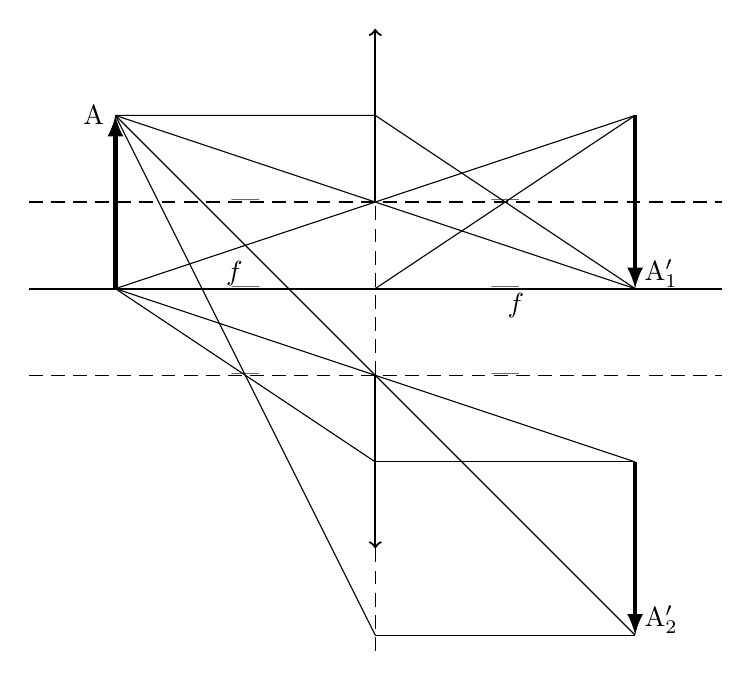
\begin{tikzpicture}[scale=0.55]

 % Def. koordinaadid
 \coordinate (O) at (0,0) ;
 \coordinate (A) at (-8,0) ;
 \coordinate (A') at (8,0) ;
 \coordinate (1) at (0,2);
 \coordinate (2) at (0,6);
 \coordinate (3) at (0,-2);
 \coordinate (4) at (0,-6);
 \coordinate (K) at (-6,4);
 \coordinate (KO) at (-6,0);
 

 % Jooned, t2pid
 \draw[thick] (A) -- (A');
 \draw[thick][->] (1) -- (2);
 \draw[thick][->] (3) -- (4);
 \draw[dash pattern=on5pt off3pt] (-8,2) -- (8,2);
 \draw[dash pattern=on5pt off3pt] (-8,-2) -- (8,-2);
 \draw[dash pattern=on5pt off3pt] (0,-2) -- (0,2);
 \draw[dash pattern=on5pt off3pt] (0, -6) -- (0,-8.5);
 \draw (K) -- (6,0);
 \draw (K) -- (0,4);
 \draw (6,0) -- (0,4);
 
 \draw (KO) -- (6,4);
 \draw (0,0) -- (6,4);
 
 \draw (KO) -- (6,-4);
 \draw (KO) -- (0,-4);
 \draw (6,-4) -- (0,-4);
 
 \draw (K) -- (6,-8);
 \draw (K) -- (0,-8);
 \draw (0,-8) -- (6,-8);
 
 \pgfsetarrowsstart{latex}
 \draw[ultra thick] (K) -- (KO) ;
 \draw[ultra thick] (6,0) -- (6,4) ;
 \draw[ultra thick] (6,-8) -- (6,-4) ;

 % Nurgad ja punktid
 \node[] at (-6.5,4) {A};
 \node[] at (-3,0) {|};
 \node[] at (3,0) {|};
 \node[] at (-3,2) {|};
 \node[] at (3,2) {|};
 \node[] at (-3,-2) {|};
 \node[] at (3,-2) {|};
 \node[] at (3.25,-0.4) {$f$};
 \node[] at (-3.25,0.35) {$f$};
 \node[] at (6.6,0.35) {$\mathrm{A_1'}$};
 \node[] at (6.6,-7.65) {$\mathrm{A_2'}$};
 
\end{tikzpicture}
\end{center}
\probend
\bigskip

% L106
\setAuthor{Taavi Pungas}
\setRound{lahtine}
\setYear{2012}
\setNumber{G 4}
\setDifficulty{3}
\setTopic{Geomeetriline optika}

\prob{Kärbes}
\solu
Kärbse trajektoor lühikese aja $t$ jooksul on sirgjoon pikkusega $h=vt$. Konstrueerime joonisel kärbse kujutise trajektoori. Sarnastest kolmnurkadest saame leida kujutise trajektoori pikkuse $h'$:
$$\frac{h}{a-f}=\frac{h'}{f} \Rightarrow h'=\frac{f}{a-f} h.$$
Kujutise kiirus on seega
$$v' = \frac{h'}{t} = \frac{f}{a-f} \frac{h}{t} = \frac{f}{a-f} v. $$
ning see on vastassuunaline kärbse kiirusega.
\probend
\bigskip

% L107
\setAuthor{Oleg Košik}
\setRound{piirkonnavoor}
\setYear{2012}
\setNumber{G 1}
\setDifficulty{3}
\setTopic{Geomeetriline optika}

\prob{Peegel}
\solu
\begin{center}
\includegraphics[width=200pt]{2012-v2g-01-peegel_lah}
\end{center}

Joonisel on kujutatud hetk $t$, mil tuttavad märkavad teineteist. Selleks hetkeks läbis $A$ teepikkuse $2-1\cdot t$ ning $B$ läbis teepikkuse $\num{3,5}-1\cdot t$. Sarnastest kolmnurkadest saame
\[
\frac{1}{\num{3,5}-t}=\frac{2-t}{1}.
\]
Tekib ruutvõrrand, mille lahenditeks on $t=\SI{1,5}{s}$ ja $t=\SI{4,0}{s}$, neist vastuseks on esimene lahend.
\probend
\bigskip

% L108
\setAuthor{Tanel Kiis}
\setRound{lõppvoor}
\setYear{2013}
\setNumber{G 1}
\setDifficulty{3}
\setTopic{Geomeetriline optika}

\prob{Läätsed}
\solu
\begin{center}
	\includegraphics[width=0.8\textwidth]{2013-v3g-01-laats_lah2}\\
\end{center}
Kogu pilt on optilise peatelje suhtes sümeetriline, tänu sellele saame tegeleda ainult ühe poolega. Konstrueerime kiirte käigu, teades et kõigi nõgusläätse läbivate paraleelsete kiirte pikendused lõikuvad fokaaltasandil. 

Joonisel on mõned meid huvitavad sarnased kolmnurgad: $$\Delta AF'D \sim \Delta BO'D \sim \Delta CFD$$ ja $$\Delta EOF \sim \Delta AF'O' \sim \Delta BO'F.$$ Lisaks teame osade lõikude pikkusi: $|EO| = R$, $|OF| = f_1$, $|F'O'| = f_2$ ja $|CF| = r$.
Seda teades saab moodustada neljast võrrandist koosneva lineaarvõrrandisüsteemi.
\[ 
\begin{cases}
\frac{|EO|}{|OF|} = \frac{|AF'|}{F'O}\\
\frac{|EO|}{|OF|} = \frac{|BO'|}{O'F}\\
\frac{|AF'|}{|F'D|} = \frac{|CF|}{|FD|}\\
\frac{|AF'|}{|F'D|} = \frac{|BO'|}{|O'D|},\\
\end{cases}
\]
\[ 
\begin{cases}
\frac{R}{f_1} = \frac{|AF'|}{f_2}\\
\frac{R}{f_1} = \frac{|BO'|}{\frac{f_1}{2}}\\
\frac{|AF'|}{|O'D| - f_2} = \frac{r}{\frac{f_1}{2} + |O'D|}\\
\frac{|AF'|}{|O'D| - f_2} = \frac{|BO'|}{|O'D|}.\\
\end{cases}
\]

Pärast süsteemi lahendamist saame tulemuseks $f_2 = \frac{R}{4r}f_1$. 

\vspace{0.5\baselineskip}
\emph{Alternatiivne lahendus}\\

\begin{center}
	\includegraphics[width=0.9\textwidth]{2013-v3g-01-laats_lah3}\\
\end{center}

Selles lahenduses kasutame läätse valemit $-\frac{1}{f} = \frac{1}{a} - \frac{1}{k}$. $f$ ees on miinus, kuna tegemist on nõgusläätsega, ja $k$ ees on miinus, kuna tegemist on näiva kujutisega. Kasutades kiirte pööratavuse printsiipi vaatame hoopis olukorda, kus tekib objektist $CF$ näiv kujutis $AB$. Lisaks kasutame kolmnurkade sarnasust: $\Delta CFO' \sim \Delta ABO'$ ja $\Delta DOF \sim \Delta ABF$.

\[ 
\begin{cases}
\frac{|CF|}{|FO'|} = \frac{|AB|}{|BO'|}\\
\frac{|DO|}{|OF|} = \frac{|AB|}{|BF|}\\
-\frac{1}{f_2} = \frac{1}{|FO'|} - \frac{1}{|BO'|},\\
\end{cases}
\]
\[ 
\begin{cases}
\frac{r}{\frac{f_1}{2}} = \frac{|AB|}{|BO'|}\\
\frac{R}{f_1} = \frac{|AB|}{\frac{f_1}{2} - |BO'|}\\
-\frac{1}{f_2} = \frac{1}{\frac{f_1}{2}} - \frac{1}{|BO'|}.\\
\end{cases}
\]
Selle võrrandisüsteemi lahendamisel saame $f_2 = \frac{R}{4r}f_1$.
\probend
\bigskip

% L109
\setAuthor{Valter Kiisk}
\setRound{lõppvoor}
\setYear{2015}
\setNumber{G 2}
\setDifficulty{3}
\setTopic{Geomeetriline optika}

\prob{Valgustamine}
\solu
Vaatleme kõige äärmiste valguskiirte liikumist läbi süsteemi. 
\begin{center}
\includegraphics[scale=1.5]{2015-v3g-02-valgustamine-lah}
\end{center}
Pärast lisaläätse läbimist koonduvad valguskiired punktiks lisaläätsest kaugusel $f_2$ ehk kaugusel $L-f_2$ algsest läätsest. Läätse valemi 
\begin{equation}
\frac{1}{a}+\frac{1}{L-f_2}=\frac{1}{f_1}.
\end{equation}
põhjal tekib sellest punktist omakorda punktkujutis kaugusele $a$ esimesest läätsest. Sarnastest kolmnurkadest saame veel kaks võrrandit:
\begin{equation}
\frac{d_1}{d_0}=\frac{L-f_2}{f_2},
\end{equation}
\begin{equation}
\frac{d}{a-f_1}=\frac{d_1}{a}.
\end{equation}
Kahest esimesest võrrandist saame suuruse $\frac{1}{L-f_2}$ avaldamisel
\begin{equation}
\frac{1}{a}+\frac{d_0}{d_1f_2}=\frac{1}{f_1}\implies \frac{d_0}{d_1f_2}=\frac{a-f_1}{af_1}.
\end{equation}
Viimasest kahest võrrandist saame avaldada suuruse $d_1(a-f_1)/a$, mille põhjal saame $d=d_0\frac{f_1}{f_2}.$ Seega valguslaigu suurus ekraanil sõltub ainult lisatud läätse fookuskaugusest, aga mitte läätsedevahelisest kaugusest $L$. Valguslaik diameetriga \SI{2}{cm} tekib kui $f_2=f_1d_0/d=\SI{2}{cm}$.
\probend
\bigskip

% L110
\setAuthor{Andreas Valdmann}
\setRound{lahtine}
\setYear{2016}
\setNumber{G 4}
\setDifficulty{4}
\setTopic{Geomeetriline optika}

\prob{Optiline kiud}
\solu
Pikas optilises kius jäävad levima vaid sellised kiired, mille jaoks toimub südamiku ja katte lahutuspinnal täielik sisepeegeldumine. Kui valgus langeb lahutuspinnale täieliku sisepeegeldumise piirnurgast väiksema nurga all, siis toimub korraga nii peegeldumine kui ka murdumine. Pärast mitmeid peegeldusi väheneb nende kiirte intensiivsus praktiliselt nullini, sest peaaegu kogu valgus on kiu külgedelt välja murdunud. Täieliku sisepeegeldumise piirnurk 
\[
\alpha=\arcsin(n_2/n_1)=\ang{80,5}.
\]
Piirnurgale vastavad kiired levivad kiu telje suhtes nurga $\ang{90}-\alpha$ all. Pärast kiu otsast väljamurdumist on nende kiirte nurk kiu telje suhtes 
\[
\beta=\arcsin[n_1\sin(\ang{90}-\alpha)]=\arcsin[n_1\cos(\alpha)].
\]
Valguskoonuse tipunurk $\theta$ on sellest kaks korda suurem: 
\[
\theta=2\beta=2\arcsin[n_1\cos(\alpha)]=\ang{28}.
\]
Kuna $\cos(\arcsin(a))=\sqrt{1-a^2}$, siis on võimalik vastus esitada kujul 
\[
\theta=2\arcsin(\sqrt{n_1^2-n_2^2}).
\]

\begin{center}
 \includegraphics[width=0.35\textwidth]{2016-lahg-04-kiud}
\end{center}
\probend
\bigskip

% L111
\setAuthor{Andres Põldaru}
\setRound{lahtine}
\setYear{2016}
\setNumber{G 5}
\setDifficulty{4}
\setTopic{Geomeetriline optika}

\prob{Kolmlääts}
\solu
Kõigil kolmel läätsel on sama fookuskaugus, sest neil on üks ühine fookuspunkt, milleks on kolmnurga keskpunkt. Kolmnurgad $\triangle ACD$ ja $\triangle CEF$ on sarnased, sest nad on täisnurksed kolmnurgad, mille ühise tipu $C$ juures olevad nurgad on samad. Seega 
\[
\frac{|AD|}{|AC|}=\frac{|EF|}{|EC|},
\]
millest
\[
|AD| = \frac{|AC|}{2} = f.
\]

\begin{center}
	{\def\l{5}
	\pgfmathsetmacro\cos{cos(30)}
	\pgfmathsetmacro\tan{tan(30)}
	\begin{tikzpicture}[scale=0.7]
	\coordinate (A) at (-\l*\tan,0);
	\coordinate (B) at (\l*\cos+\l/2*\tan,0);
	\draw[Stealth-Stealth] (0,0) node[below]{C} -- ++(30:5) node[above]{E};
	\draw[Stealth-Stealth] (30:\l) -- ++(-90:5) node[below]{G};
	\draw[Stealth-Stealth] (0,0) -- ++(-30:\l);
	\draw (0,0) -- ++(210:2.5) node[below]{D} -- ++(30:0.3) arc (30:120:0.3) -- ++(-60:0.3)-- (A) -- (0,0) -- (\l*\cos,0) node[below left]{F};
	\node at (B) {\textbullet} (B) node[anchor=west] {B};
	\node at (A) {\textbullet} (A) node[anchor=east] {A};
	\draw[decorate,decoration={brace,raise=2pt,amplitude=6pt}] (A) -- node[above right = 7pt and -10pt]{$2f$} (0,0) ;
	\draw[decorate,decoration={brace,raise=2pt,amplitude=6pt}] (210:2.5) -- node[below left = 2pt and 6pt]{$f$} (A);
	\draw[decorate,decoration={brace,raise=2pt,amplitude=6pt}] (B) -- node[below right = 7pt and -8pt]{$f$} (\l*\cos,0) ;
	\end{tikzpicture}}
\end{center}

Saame järeldada, et punkt $A$ asub mõlema läätse $CE$ ja $CG$ fokaaltasandites. Kui läätsele langevad paralleelsed kiired, siis need koonduvad fokaaltasandis ühte punkti ja seega teistpidi mõeldes peavad fokaaltasandi ühest punktist pärinevad kiired olema pärast läätse läbimist paralleelsed. Nende paralleelsete kiirte nurka on võimalik määrata nii, et tõmbame punktist $A$ ühe kiire läbi läätse $CE$ või $CG$ keskpunkti. Läätse keskpunkti läbiv kiir ei murdu ja liigub samas suunas edasi. Alumisel joonisel läbib kiir $AH$ läätse keskpunkti ja teised kiired on konstrueeritud selliselt, et pärast läätse läbimist on nad sellega pralleelsed.

Pärast esimese läätse läbimist koonduvad läätsele $EG$ langevad paralleelsed kiired fokaaltasandi ühte punkti $J$. Selle punkti leidmiseks joonistame läätse $EG$ keskpunkti $F$ läbiva kiire, mis on kiirega $AH$ paralleelne, ja leiame selle kiire lõikumispunkti $J$ fokaaltasandiga. Jooniselt on näha, et ükski kiir punkti $B$ ei jõua, sest nad kõik kõik koonduvad punkti $J$ ja vertikaalseid kiiri ei ole. Läätse $CG$ jaoks on konstruktsioon sama, ainult peegelpildis $AB$ suhtes ja seega ka sealt ei jõua valgus punkti $B$.

\begin{center}
	{\def\l{5}
	\pgfmathsetmacro\cos{cos(30)}
	\pgfmathsetmacro\tan{tan(30)}
	\begin{tikzpicture}[scale=0.9]
	\usetikzlibrary{calc};
	\pgfmathsetmacro\tanb{sqrt(3)/7}
	\pgfmathsetmacro\k{\l*\cos+\l*\tan}
	\coordinate (A) at (-\l*\tan,0);
	\coordinate (B) at (\l*\cos+\l/2*\tan,0);
	\coordinate (H) at ($\k*(1,\tanb)+(A)$);
	\coordinate (J) at ($(\l*\cos,0)+\l*\tan/2*(1,\tanb)$);
	\draw[Stealth-Stealth] (0,0) node[below left]{C} -- ++(30:5) node[above]{E};
	\draw[Stealth-Stealth] (30:\l) -- ++(-90:5) node[below]{G};
	\draw[Stealth-Stealth] (0,0) -- ++(-30:5);
	\node at (B) {\textbullet} (B) node[anchor=west] {B};
	\node at (A) {\textbullet} (A) node[anchor=east] {A};
	\draw (A) -- (H) node{\textbullet} node[above left = -3pt and 0pt]{H};
	\draw (\l*\cos,0) node[left]{F} -- (J) node {\textbullet} node[above right = -5pt and 0pt]{J};
	\draw (H) -- (J);
	\draw (A) -- (30:0.5) -- ++({(\l-0.5)*\cos},{(\l-0.5)*\cos*\tanb}) -- (J);
	\draw (A) -- (30:4.5) -- ++({(\l-4.5)*\cos},{(\l-4.5)*\cos*\tanb}) -- (J);
	\end{tikzpicture}}
\end{center}

\emph{Alternatiivne lahendus}\\
Analoogselt võime vaadata hoopis seda, kui punktis $B$ on valgusallikas. Kui punktist $A$ pärinevad kiired jõuavad punkti $B$, siis peavad ka punktist $B$ pärinevad kiired jõudma punkti $A$. Punkt $B$ on läätse $EG$ fokaaltasandis ja tekitab paralleelse kiirtekimbu. Sarnaselt eelmise lahendusega see kiirtekimp koondub pärast teise läätse läbimist selle läätse fokaaltasandi ühte punkti, mis ei ole $A$. Fokaaltasand on läätsega paralleelne ja kui kiired koonduvad selles tasandis mingisse punktist $A$ erinevasse punkti, siis järelikult punkti $A$ valgus ei jõua.
\probend
\bigskip

% L112
\setAuthor{Eero Vaher}
\setRound{piirkonnavoor}
\setYear{2017}
\setNumber{G 5}
\setDifficulty{4}
\setTopic{Geomeetriline optika}

\prob{Puuduv lääts}
\solu
Nõguslääts tekitab esemest näiva kujutise ning kumerlääts tekitab näivast kujutisest tõelise kujutise. Teades kumerläätse asukohta ja fookuseid ning tõelise kujutise asukohta, on võimalik leida näiva kujutise asukoht (joonisel kujutatud sinisega; kujutatud on kolme kiirt, kuid konstrueerimiseks piisab kahest). Teades eseme ning nõgusläätse tekitatud näiva kujutise asukohti, on läätse asukoha ning selle esemepoolse fookuse leidmine lihtne. 

\begin{resizebox}{\linewidth}{!}{
		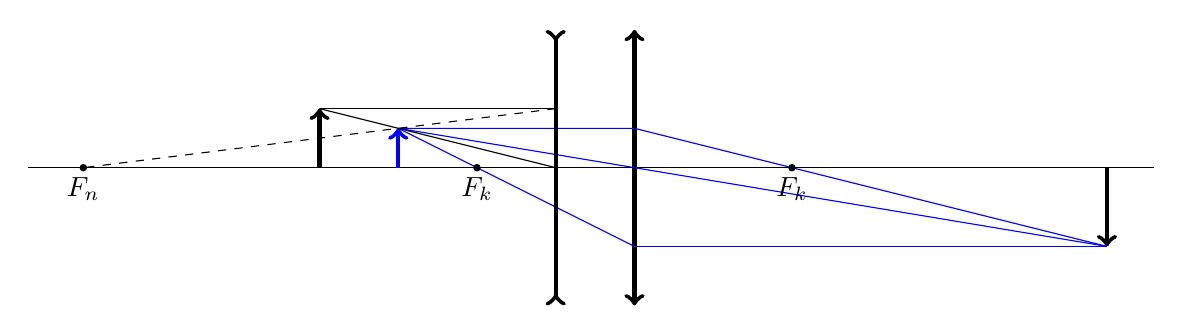
\begin{tikzpicture}
		\pgfmathsetmacro{\fk}{2}
		\pgfmathsetmacro{\tk}{3*\fk}
		\pgfmathsetmacro{\nk}{1/(1/\fk-1/\tk)}
		\pgfmathsetmacro{\a}{2*\fk}
		\pgfmathsetmacro{\h}{0.5}
		\pgfmathsetmacro{\htk}{\tk/\nk*\h}
		\pgfmathsetmacro{\ha}{1.5*\h}
		\pgfmathsetmacro{\nl}{\nk-\h/(\h-\ha)*(\nk-\a)}
		\pgfmathsetmacro{\fn}{\nk-\h/(\h-\ha)*(\nk-\nl)}
		\coordinate (TK) at (\tk, -\htk);
		\coordinate (NK) at (-\nk, \h);
		\coordinate (A) at (-\a, \ha);
		\draw (-1.1*\fn, 0) -- (1.1*\tk, 0);
		\draw[<->, ultra thick] (0,3.5*\h) -- (0,-3.5*\h);
		\draw[->, ultra thick] (\tk, 0) -- (TK);
		\draw[->, ultra thick, blue] (-\nk, 0) -- (NK);
		\draw[blue] (TK) -- (NK);
		\draw[blue] (TK) -- (0,-\htk);
		\draw[blue] (0,-\htk) -- (NK);
		\draw[blue] (TK) -- (0,\h) -- (NK);
		\draw[fill] (-\fk, 0) circle (0.02*\fk) node[below] {$F_k$};
		\draw[fill] (\fk, 0) circle (0.02*\fk) node[below] {$F_k$};
		\draw[->, ultra thick] (-\a, 0) -- (A);
		\draw[>-<, ultra thick] (-\nl, 3.5*\h) -- (-\nl, -3.5*\h);
		\draw (-\nl, 0) -- (A) -- (NK);
		\draw (A) -- (-\nl, \ha);
		\draw[dashed] (-\nl, \ha) -- (-\fn,0);
		\draw[fill] (-\fn, 0) circle (0.02*\fk) node[below] {$F_n$};
		\end{tikzpicture}}
\end{resizebox}
\probend
\bigskip

% L113
\setAuthor{Andreas Valdmann}
\setRound{lõppvoor}
\setYear{2014}
\setNumber{G 4}
\setDifficulty{5}
\setTopic{Geomeetriline optika}

\prob{Periskoopprillid}
\solu
\osa Kuna sisenevad ja väljuvad kiired on prisma pinnaga risti, siis keskkondade lahutuspiiril nende suund ei muutu. Kui kiir langeb prismale lõigul $AB$, siis peegeldub see esmalt prisma ülemisel tahul, seejärel alumisel tahul ning väljub prismast läbi parempoolse tahu (vt joonist). Kui kiir langeb prismale lõigul $BC$, siis peegeldub see ülemisel tahul, siis parempoolsel tahul ning väljub läbi alumise tahu ja ei jõuagi silma. Kui kiir langeb prismale lõigul $CD$, siis peegeldub see esmalt parempoolsel tahul, seejärel ülemisel tahul ning väljub jällegi läbi alumise tahu.

\begin{center}
 \includegraphics[width=0.8\textwidth]{2014-v3g-04-periskoopprillid_lahendus_joonis1.pdf}
\end{center}

\osa Vaatleme kiirt, mis siseneb prismasse lõigul $AB$. Kuna sisenev kiir on pinnaga risti, siis tekib täisnurkne kolmnurk $AKL$ (vt joonist). Kolmnurga üheks teravnurgaks on $\varphi$ ja seega on teise teravnurga suurus $\ang{90}-\varphi$. Kuna viimane nurk on esimesel peegeldumisel langemisnurga täiendnurgaks, siis on ka langemisnurk $\varphi$. Peegeldumisseadusest järeldub, et esimene peegeldumisnurk on samuti $\varphi$. Kuna prismast väljuv kiir on paralleelne prisma ülemise tahuga, siis on teisel peegeldumisel peegeldumisdumisnurga täiendnurk ja seega ka langemisnurga täiendnurk $\varphi$. Näeme, et täisnurkse kolmurga $KLM$ teravnurgad on $\varphi$ ja $2\varphi$. Kuna kolmnurga sisenurkade summa on \ang{180}, siis $\varphi=(\ang{180}-\ang{90})/3=\ang{30}$.

\begin{center}
 \includegraphics[width=0.65\textwidth]{2014-v3g-04-periskoopprillid_lahendus_joonis2.pdf}
\end{center}

\emph{Märkus.} Nüüd, kui prisma tipunurk on leitud, saame veenduda, et kui pinnaga risti sisenenud kiir peegeldub prisma alumiselt või parempoolselt tahult, siis on need peegeldumised täielikud. Eelmisest alaülesandest on näha, et nendel juhtudel on langemisnurgaks $\ang{90}-\varphi=\ang{60}$. Täieliku sisepeegeldumise piirnurk on $\alpha=\arcsin(1/n)=\ang{42}$. Langemisnurk \ang{60} on sellest suurem ehk toimub täielik sisepeegeldumine.

\osa Kui kiir siseneb prismasse punktis $B$, siis läbib väljuv kiir punkti $D$ (vt joonist).

\emph{Märkus.} Väljuva kiire suund pole sel juhul üheselt määratud, kuid see ei oma ülesande lahendamisel tähtsust.\\
Kasutades eelmises alaülesandes saadud $\varphi$ väärtust, on näha, et kolmnurgad $ABL$ ja $BDL$ on teineteise peegeldused lõigu $BL$ suhtes (öeldakse, et need kolmnurgad on kongruentsed). Seega on lõikude $AB$ ja $BD$ pikkused võrdsed, millest järeldub, et $|AB|=l/2$. Kui kiir siseneb prismasse punktis $C$, siis peegeldub see punktis $O$ otse tagasi ning väljub prismast punktis $C$. Täisnurksetest kolmnurkadest saame, et $|AO|=\cos(\ang{30})|AD|$ ja $|AC|=\cos(\ang{30})|AO|$ ehk punkti $C$ kaugus punktist $A$ on 
\[
|AC|=\cos^2(\ang{30})|AD|=\frac{3}{4}l.
\]

\begin{center}
 \includegraphics[width=0.65\textwidth]{2014-v3g-04-periskoopprillid_lahendus_joonis3.pdf}
\end{center}

\osa Ühe tasapeegli kasutamisel paistab tekst peegelpildis. Seetõttu tuleb teksti õigetpidi nägemiseks kasutada süsteemi, kus toimub paarisarv peegeldusi.
\probend
\bigskip

% L114
\setAuthor{Mihkel Kree}
\setRound{lahtine}
\setYear{2015}
\setNumber{G 5}
\setDifficulty{5}
\setTopic{Geomeetriline optika}

\prob{Lääts}
\solu
Paneme esmalt tähele, et läätse keskpunkti läbivad kiired AA' ja BB' ei murdu. Seega paikneb läätse keskpunkt O lõikude AA' ja BB' lõikepunktis. Teisalt märkame, et valguskiir AB murdub valguskiireks A'B'. Niisiis, pikendades lõike AB ja A'B', leiame nende lõikepunkti X. Sellega oleme konstrueerinud läätse tasandi OX. Läätse optilise peatelje leiame, kui tõmbame läätse tasandiga ristuva sirge s läbi läätse keskpunkti O. Fookuse F leidmiseks konstrueerime näiteks peateljega paralleelse kiire AC, mis murdub läbi fookuse.

\begin{center}
\includegraphics[width=\textwidth]{2015-lahg-05-laatsLahendus.pdf}
\end{center}
\probend
\bigskip

% L115
\setAuthor{Sandra Schumann}
\setRound{lõppvoor}
\setYear{2018}
\setNumber{G 3}
\setDifficulty{5}
\setTopic{Geomeetriline optika}

\prob{Peegelpõhi}
\solu
Paneme tähele, et valemi järgi, kui keskkonna murdumisnäitaja suureneb, aga läätse murdumisnäitaja jääb samaks, siis läätse fookuskaugus suureneb. Seega on ainus viis, kuidas valguskiired saaksid ka pärast anuma vett täis valamist samas punktis koonduda, see, kui vee sees valguskiired peegelduksid põhjas olevalt peeglilt ja seejärel koonduksid samas punktis, kus enne.

Läätse kaugus anuma põhjast on $l = \SI{10}{cm}$. Olgu läätse fookuskaugus õhus $f$. Siis on tema fookuskaugus vees järelikult $2l-f$. Valemi põhjal saame, et
\[ \frac{f}{2l-f} = \frac{n_k n_0 - n_0 n_v}{n_k n_v - n_0 n_v}\Rightarrow \]
\[ f(n_k n_v - n_0 n_v) = (2l-f)(n_k n_0 - n_0 n_v)\Rightarrow \]
\[ n_k n_v f - n_0 n_v f = 2l n_k n_0 - 2l n_0 n_v - n_k n_0 f + n_0 n_v f\Rightarrow \]
\[ f (n_k n_v + n_k n_0 - 2 n_0 n_v) = 2l n_0 (n_k - n_v)\Rightarrow \]
\[ f = \frac{2l n_0 (n_k - n_v)}{n_k n_v + n_k n_0 - 2 n_0 n_v}. \]
Seega on läätse fookuskaugus 
\[ f = \frac{\num{2} \cdot \SI{10}{cm} \cdot \num{1,0} \cdot (\num{1,49} - \num{1,33})}{\num{1,49}
\cdot \num{1,33} + \num{1,49} \cdot \num{1,0} - \num{2} \cdot \num{1,0} \cdot \num{1,33}} = \SI{3,94}{cm}
\approx \SI{4}{cm}. \]
\probend
\bigskip

% L116
\setAuthor{Eero Vaher}
\setRound{piirkonnavoor}
\setYear{2015}
\setNumber{G 8}
\setDifficulty{6}
\setTopic{Geomeetriline optika}

\prob{Fookuskaugus}
\solu
Langegu läätsele vasakult valguskiir, mille suund on paralleelne optilise teljega ning mille kaugus sellest on $d$. Läätse sisenedes valgus oma levimissuunda ei muuda, kuna langeb läätsele selle pinnaga risti. Hõbetatud pind toimib kumerpeeglina, mille fookuskaugus on $\frac{R}{2}$. Kui peegeldunud valguskiire nurk optilise peatelje suhtes on $\alpha$, siis läätsest väljunud kiire ning optilise peatelje vaheline nurk on murdumisseaduse põhjal $\sin\gamma=n\sin\alpha$. Kuna lääts on õhuke, asetsevad punktid, kus valguskiir peegeldus ning kus see murdus, üksteisele väga lähedal. Seetõttu võime kirjutada
\[ d=\frac{R}{2}\tan\alpha=f\tan\gamma. \]
Õhukese läätse korral on selle nõgusa osa kõverusraadius oluliselt suurem fookuskaugusest, mis lubab kasutada väikeste nurkade lähendust ehk $\alpha\approx\sin\alpha\approx\tan\alpha$ ning $\gamma\approx\sin\gamma\approx\tan\gamma$. Tulemuseks saame
\[ f=\frac{R}{2n}. \]
Tasub teada, et avaldis sfäärilise peegli fookuskauguse jaoks kehtibki ainult väikeste peegeldumisnurkade korral. Suurte peegeldumisnurkade korral ilmneb sfääriline aberratsioon ning ei ole võimalik rääkida ühest fookusest.

\begin{center}
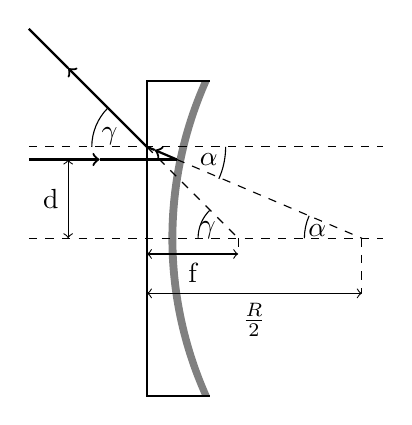
\begin{tikzpicture}[scale=1]
\def\tmp{65.92}
\fill [gray] (0.7,2) arc (90+\tmp:270-\tmp:4.9) -- (0.8,-2) -- (0.8,-2) arc (270-\tmp:90+\tmp:4.9) -- (0.7,2);
\draw[thick] (0.8,-2) -- (0,-2) -- (0,2) -- (0.8,2);
\draw[dashed] (-1.5,0) -- (3,0);
\draw[->,thick] (-1.5,1) -- (-0.6,1);
\draw[thick] (-0.6,1) -- (0.38,1);
\draw[dashed] (0.38,1) -- (2.73,0);
\draw[->,thick] (0.38,1) -- (0.1,1.12);
\draw[thick] (0.1,1.12) -- (0,1.16);
\draw[->,thick] (0,1.16) -- (-1,2.16);
\draw[thick] (-1,2.16) -- (-1.5,2.66);
\draw[dashed] (0,1.16) -- (1.16,0);
\draw[<->] (-1,0) -- (-1,1);
\node [left] at (-1,0.5) {d};
\draw[dashed] (-1.5,1.16) -- (3,1.16);
\node [left] at (-0.25,1.3) {$\gamma$};
\draw (-0.7,1.16) arc (180:135:0.7);
\node [right] at (0.55,1) {$\alpha$};
\draw (1,1.16) arc (0:-24:1);
\draw[dashed] (1.16,0) -- (1.16,-0.2);
\draw[<->] (0,-0.2) -- (1.16,-0.2);
\node [below] at (0.58,-0.2) {f}; 
\draw[dashed] (2.73,0) -- (2.73,-0.7);
\draw[<->] (0,-0.7) -- (2.73,-0.7);
\node[below] at (1.36,-0.7) {$\frac{\text{R}}{2}$};
\node[left] at (2.4,0.1) {$\alpha$};
\draw (2,0) arc (180:156:0.7);
\node[left] at (1,0.1) {$\gamma$};
\draw (0.65,0) arc (180:135:0.5);
\end{tikzpicture}
\end{center}
\probend
\bigskip

% L117
\setAuthor{Jaan Kalda}
\setRound{lõppvoor}
\setYear{2012}
\setNumber{G 6}
\setDifficulty{7}
\setTopic{Geomeetriline optika}

\prob{Toru}
\solu
Kõigepealt paneme tähele, et punktallika kujutis tekib läätsest kaugusele
$$l=\left(\frac 1{36}-\frac 1{60}\right)^{-1}\SI{}{mm}=\SI{90}{mm},$$
st ekraanil. Kui peegeldavate silindriliste seinte asemel oleks kaks tasapeeglit, siis
tekiks punktallika kujutiste lõpmatu jada (peegeldus, peegelduse peegeldus jne), kus 
kahe naaberkujutise vahekaugus on võrdne peeglite vahekaugusega \SI{12}{mm}. 
Läheme nüüd silindrilise juhtumi juurde. Joonise tasandis lebava kiire jaoks on 
kiirekäik täpselt sama, mis tasapeegli puhul, st joonise tasandis tekivad kujutised samuti 
perioodilise rivina, kus kujutiste vahekaugus on \SI{12}{mm}. Joonise tasandit võib pöörata suvaliselt
ümber süsteemi sümmeetriatelje; see tähendab, et kujutised on tegelikult \enquote{laiali määritud} mööda kontsentrilisi
ringjooni raadiustega $n\times\SI{12}{mm}$, kus $n$ on täisarv. Lääts tekitab neist ringidest 
ekraanile $\frac{90}{60}$ korda suurendatud kujutise, 
kus kontsentriliste ringide raadiusteks on $R=n\times \SI{18}{mm}$.
\probend
\bigskip

% L118
\setAuthor{Valter Kiisk}
\setRound{lõppvoor}
\setYear{2013}
\setNumber{G 7}
\setDifficulty{7}
\setTopic{Geomeetriline optika}

\prob{Mikroskoop}
\solu
Esimeses teravustatavas asendis, kus lääts on objektile lähemal kui sensorile (st suurendus $>1$), olgu läätse kaugus esemest $a$ ja sensorist $b$. Kujutise joonsuurendus on seega $k=b/a$. Teises asendis on nimetatud kaugused lihtsalt ümbervahetatud ja suurendus vastavalt $l=a/b$. Niisiis $25=k/l=b^2/a^2$.

Analüüsime nüüd esimesele asendile vastavate kauguste näitel sensori valgustatuse küsimust. Kuivõrd joonsuurendus on $k$, siis pindalamuutust iseloomustav tegur on vastavalt $k^2$. Lisaks kujutise suurusele mõjutab selle heledust ka valguse hulk, mis pääseb läbi objektiivi. Vaadeldava eseme igast punktist lähtub valgus, mis on enam-vähem ühtlaselt hajutatud üle kõigi suundade, seega läätse läbiva kiirguse hulk on proportsionaalne selle osaga mõttelise sfääri pinnast, mille lõikab välja läätse apertuur: $\Omega=d^2/a^2$, kus $d$ on läätse diameeter. Kokkuvõttes saame, et kujutise heledus on võrdeline suurusega $\Omega/k^2=d^2/b^2\propto b^{-2}$. Teises asendis, kus lääts on sensorile lähemal, on sama näitaja vastavalt $a^{-2}$, seega sel juhul on kujutise heledus suurem $a^{-2}/b^{-2}=b^2/a^2=25$ korda.
\probend
\bigskip

% L119
\setAuthor{Erkki Tempel}
\setRound{lahtine}
\setYear{2014}
\setNumber{G 7}
\setDifficulty{7}
\setTopic{Geomeetriline optika}

\prob{Optiline skeem}
\solu
\begin{center}
\includegraphics[width=0.7\textwidth]{2014-lahg-07-optilineskeemlahendus}
\end{center}
Algselt paralleelsed kiired koonduvad pärast läätse läbimist fokaaltasandis (punkt A). Kuna alumine kiir ei murdu, peab see läbima läätse keskpunkti. Seega lääts 1 on paralleelne joonistatud fokaaltasandiga (kiir läbib punkte A ja F) ning läbib punkti $\text{O}_1$. Kuna tegemist on kahe ühesuguse läätsega ning nende fookused asuvad punktis F, siis ring raadiusega $\text{FO}_1$ läbib alumist kiirt punktis $\text{O}_2$, mis on teise läätse keskpunktiks. Nüüd saame kergesti joonistada ka teise läätse, kuna teame ülemise kiire murdumiskohta ning läätse keskpunkti asukohta.
\probend
\bigskip

% L120
\setAuthor{Valter Kiisk}
\setRound{lõppvoor}
\setYear{2016}
\setNumber{G 6}
\setDifficulty{7}
\setTopic{Geomeetriline optika}

\prob{Luup}
\solu
Poolkera kumera pinna keskosa võib vaadelda omaette õhukese läätsena, mille fookuskaugus $f$ ja kaugus paberi pinnast (võrdne kumerpinna raadiusega $R$) määravad kujutise suurenduse. Selle ekvivalentse läätse fookuskauguse määramiseks vaatleme valguskiirt, mis liigub paralleelselt optilise peateljega ja pärast murdumist koondub fookusesse (vt joonis). Kui valguskiir levib optilise peatelje lähedal, siis kõik murdumisel tekkivad nurgad on väikesed, nii et saame tingimuse
\[
\alpha R\approx f\varphi.
\]
Ilmselt
\[
\varphi = \alpha - \beta=\alpha-\alpha/n=\alpha(1-1/n).
\]
Nende seoste kombineerimisel nurgad taanduvad välja ja saame $f=nR/(n-1)$. Ilmselt eseme (paberi pinna) kaugus läätsest on $R$, kusjuures $f > R$, järelikult tekib näiline kujutis kusagil paberi taga. Kõik kaugused on siiski $R$ suurusjärgus, seega suurelt distantsilt silmaga vaadeldav suurendus (st nurksuurendus) on praktiliselt sama mis joonsuurendus $y/y_0$. Kujutise konstrueerimisel tekkivatest sarnastest kolmnurkadest saame
\[
\frac{y}{y_0}=\frac{f}{f-R}=n=\num{1.5}.
\]

\begin{center}
	\includegraphics[scale=1.2]{2016-v3g-06-luup-lah}
\end{center}
\probend
\bigskip

% L121
\setAuthor{Andreas Valdmann}
\setRound{lõppvoor}
\setYear{2016}
\setNumber{G 8}
\setDifficulty{8}
\setTopic{Geomeetriline optika}

\prob{Nurgapeegel}
\solu
Vaatame kõigepealt kujutise tekkimist tasapeeglis. Joonisel 1 on olukord pealtvaates. A on Juku lahtine silm ja A$'$ selle kujutis. Kinnine silm ja selle kujutis on vastavalt B ja B$'$. Näeme, et parema silma kinnipigistamisel paistab ka peeglis kinnisena vaatleja suhtes parempoolne silm.
\begin{figure*}[h]
	\centerline{\includegraphics[scale=1.2]{2016-v3g-08-nurgapeegel_j1}}
	\caption{Kujutis tasapeeglis}
\end{figure*}

Olgu kolmest peeglist üks horisontaalne ja kaks ülejäänut vertikaalsed, kusjuures Juku vaatab otse vertikaalsete peeglite kokkupuutejoone poole. Joonisel 2 on see olukord pealtvaates. Vaatame vertikaalsete peeglite mõju. Esmalt konstrueerime silma A kujutise A$'$ vasakpoolses peeglis. Seejärel konstrueerime kujutise A$'$ kujutise A$''$ parempoolses peeglis. Toimime samamoodi kujutise B$''$ konstrueerimisel ja paneme tähele, et seekord on peegelpildil vasak ja parem pool vahetatud ning kinnisena paistab peeglites vasakpoolne silm.
\begin{figure*}[h]
	\centerline{\includegraphics[scale=1.2]{2016-v3g-08-nurgapeegel_j2}}
	\caption{Kujutis kahes peeglis}
\end{figure*}

Võtame nüüd arvesse horisontaalse peegli mõju. Joonisel 3 on otsevaates teist järku kujutis A$''$ ning selle kujutis A$'''$ horisontaalses peeglis. Näeme, et horisontaalne peegel pöörab pildi \enquote{pea peale}. Seega näeb Juku nurgapeeglis ennast sellisena, nagu on joonisel 3 kujutis A$'''$.
\begin{figure*}[h]
	\centerline{\includegraphics[scale=1.1]{2016-v3g-08-nurgapeegel_j3}}
	\caption{Peegeldumine horisontaalselt peeglilt}
\end{figure*}
\probend
\bigskip

% L122
\setAuthor{Jaan Kalda}
\setRound{lõppvoor}
\setYear{2015}
\setNumber{G 7}
\setDifficulty{9}
\setTopic{Geomeetriline optika}

\prob{Ring ja ellips}
\solu
Läätse keskpunkt $O$ on ringile ja ellipsile tõmmatud puutujate lõikepunkt, kuna puutepunktid peavad olema originaalkujutise paarid ning neid ühendavad sirged peavad läbima läätse keskpunkti. Läätse tasandi leidmiseks valime ringil kaks punkti, $A$ ja $B$, ning leiame nende kujutised ellipsil $A'$ ja $B'$ sirgete $AO$ ja $BO$ ning ellipsi lõikepunktidena. Kui originaal on ringi kahest lõikepunktist see, mis asub läätsest kaugemal, siis selle kujutis on see, mis on läätsele lähemal (ja vastupidi), sest tõeline kujutis on pööratud tagurpidi. Kiir $AB$ peab murduma läätses kiireks $A'B'$, murdepunkt annab meile punkti $L$ läätsel ning sirge $OL$ on läätse tasandiks. Optilise peatelje $o$ leiame sirgele $OL$ punktist $O$ tõmmatud ristsirgena. Fookuse leidmiseks tõmbame punktist $A$ kiire, mis on paralleelne $o$-ga ja murdub läätsel punkti $A'$ läbivaks kiireks, mille lõikepunkt $o$-ga annab fookuse $F$.

\begin{center}
\includegraphics[width=\textwidth]{2015-v3g-07-ellips_lah}
\end{center}
\probend
\bigskip

% L123
\setAuthor{Ardi Loot}
\setRound{lõppvoor}
\setYear{2017}
\setNumber{G 8}
\setDifficulty{9}
\setTopic{Geomeetriline optika}

\prob{Kaamera}
\solu
On selge, et kuna virmalised asuvad kaugel, peab terava kujutise
tekkimiseks olema valgustundlik element esialgse läätse fookuses,
st kaugusel $f=\SI{14}{cm}.$ Kuna läätse keskpunkti läbiv kiir suunda
ei muuda, saame esialgseks vaatenurgaks $2\alpha=2\arctan\left(h/f\right).$

\begin{center}
	\includegraphics[width=10cm]{2017-v3g-08-skeem__telephoto.pdf}
\end{center}
Joonisel on kujutatud kompaktse kaamera skeem. Vaatleme lihtsuse huvides
olukorda tagurpidi, vaadeldav objekt asub fototundliku elemendi asemel
ning kujutis konstrueeritakse lõpmatuses (kiirte pööratavuse printsiip).
Nõguslääts, mis on paigutatud kaugusele $d$ kumerläätsest, tekitab
objektist $A$ näiva kujutise $A'$. Seda näivat kujutist vaadeldakse
kumerläätsega, mis konstrueerib sellest kujutise lõpmatuses. Kirja
saab panna järgnevad võrrandid:
\begin{eqnarray}
\frac{1}{k_{1}}-\frac{1}{a_{1}} = \frac{1}{f_{1}}, \label{2017-v3g-08-eq:telelens-eq1}\\
k_{1}+d = f_{2},\\
a_{1}+d = L_{m}.
\end{eqnarray}

\noindent Neist esimene määrab nõgusa läätse poolt näiva kujutise asukoha.
Teine võrrand garanteerib, et kumerlääts konstrueerib sellest kujutise
lõpmatuses. Kolmas võrrand tagab, et kogu süsteem oleks kompaktne.
Lisaks eeltoodud võrranditele on vaja säilitada ka esialgse kaamera
vaatenurk. Selleks märkame, et joonisel toodud nurk $\measuredangle A'O_{2}F_{2}=\alpha.$
Seetõttu saame kirja panna:
\begin{equation}
\frac{h'}{f_{2}}=\frac{h}{f},
\end{equation}
\noindent kus $h'$ tähistab kujutise $A'$ kõrgust, mille saame leida
kolmnurkade $OAO_{1}$ ja $F_{2}A'O_{1}$ sarnasusest
\begin{equation}
h'=h\frac{k_{1}}{a_{1}.}\label{2017-v3g-08-eq:telelens-eq2}
\end{equation}

Lahendades võrranditest (\ref{2017-v3g-08-eq:telelens-eq1}) - (\ref{2017-v3g-08-eq:telelens-eq2})
tekkinud süsteemi, saame
\begin{eqnarray*}
f_{1} & = & \frac{f_{2}f(L_{m}-f_{2})}{\left(f-f_{2}\right)^{2}}\approx\SI{1.39}{cm},\\
d & = & \frac{f_{2}(f-L_{m})}{f-f_{2}}\approx\SI{1.91}{cm}.
\end{eqnarray*}
\probend
\bigskip

% L124
\setAuthor{Jaan Kalda}
\setRound{lõppvoor}
\setYear{2014}
\setNumber{G 10}
\setDifficulty{10}
\setTopic{Geomeetriline optika}

\prob{Klaassilinder}
\solu
\begin{wrapfigure}{r}{0.35\textwidth}%
\includegraphics[trim = 0mm 0mm 12mm 0mm, clip, width=1\linewidth]{2014-v3g-10-silinder}
\end{wrapfigure}

Tähistame märgitud punkti $A$-ga ning murdugu sealt lähtunud kiir punktis $B$ nii, et suundub eemale läbi punkti $C$ (vt joonist).
Sihi $BC$ suunast kaugelt vaadatuna näeme tumeda punkti asukohana punkti $B$. Uurime, kuidas sõltub kiire $BC$ levikusuund, mida kirjeldame 
$AO$ ja $BC$ vahelise nurga $2\alpha-\beta$ abil, kiire algsest levikusuunast $\alpha$:
$$2\alpha-\beta= 2\alpha-\arcsin (n\sin\alpha).$$

Silindri algasendi korral $2\alpha-\arcsin (n\sin\alpha) =0$, mille üks lahend $\alpha=0$ annab keskmise näiva punkti
ning kaks külgmist tumedat punkti vastavad võrrandi $\sin(2\alpha)=n\sin\alpha$ ülejäänud lahenditele vahemikus $-45^\circ <\alpha<45^\circ$.
Kui pöörata nüüd silindrit nurga $\delta$ võrra, siis vastavad näivad punktid võrrandi 
$$2\alpha-\arcsin (n\sin\alpha) =\delta$$
lahenditele. Võrrandi vasakul pool on funktsioon, mis väikeste nurkade puhul käitub kui $(2-n)\alpha$; suuremate nurkade puhul teise liidetava suhteline mõju kasvab.
Seega juhul $2>n$, on tegemist väikeste nurkade puhul kasvava funktsiooniga, mis läheb suuremate nurkade puhul üle kahanevaks;
juhul $2<n$ on see aga monotoonselt kahanev funktsioon. Kuivõrd $\delta=0$ puhul on kolm lahendit, siis peab olema tegemist esimese juhtumiga, $2>n$.
Nende pöördenurkade $\delta$ puhul, mis on suuremad selle funktsiooni lokaalsest maksimumist, on võrrandil vaid üks lahend.
Funktsioon saavutab globaalse maksimumi täieliku sisepeegelduse piirjuhul 
$$n\sin\alpha=-1,$$
mis annab pöördenurga
$$90^\circ-2\arcsin \frac 1n=\SI{15}{}^\circ\Rightarrow n=1/\sin \ang{37,5} = \SI{1,64}{}.$$
\probend
\bigskip

% L125
\setAuthor{Koit Timpmann}
\setRound{piirkonnavoor}
\setYear{2013}
\setNumber{G 1}
\setDifficulty{1}
\setTopic{Kinemaatika}

\prob{Rong}
\solu
Olgu rongi maksimaalne kiirus $v$ ning kogu sõiduaeg $t$. Kiirendamise jooksul on keskmine kiirus $v/2$ ning sellele kulub aega $\frac{2t}{5}$. Pidurdamine võtab aega $\frac{t}{5}$ ning ka selle jooksul on keskmine kiirus $v/2$. Kogu sõidu keskmine kiirus on seega 
$$v_k = \frac{\frac{2t}{5} \frac{v}{2}+\frac{2t}{5} v + \frac{t}{5} \frac{v}{2}}{t} = \frac{7}{10} v.$$ 
Kokku,
\[
v=\frac{10}{7}v_k \approx \SI{51}{km/h}.
\]
\probend
\bigskip

% L126
\setAuthor{Mihkel Kree}
\setRound{lahtine}
\setYear{2015}
\setNumber{G 1}
\setDifficulty{2}
\setTopic{Kinemaatika}

\prob{Rongivile}
\solu
Tähistagu $L$ veduri kaugust jaamaülemast hetkel, mil vedurijuht alustab vile laskmisega. Heli levimiseks jaamaülemani kulub sel juhul aeg $\tau_\text{A}=L/c$. Vile lõppedes on veduri kaugus jaamaülemast $L-vt_0$, kus $v$ on rongi liikumise kiirus. Heli levimiseks sellelt kauguselt kulub aeg $\tau_\text{B}=(L-vt_0)/c$. Alustagu vedurijuht vile laskmisega hetkel $\tau_0$ ning lõpetagu hetkel $\tau_0+t_0$. Jaamaülem kuuleb vile algust hetkel $\tau_0+\tau_\text{A}$ ning vile lõppu hetkel $\tau_0+t_0+\tau_\text{B}$. Nende ajahetkede vahe $t_1$ on mõistagi jaamaülema mõõdetud vile kestus. Seega saame võrrandi
\[
t_1 = t_0+\tau_\text{B}-\tau_\text{A} = t_0 - \frac{v}{c}t_0,
\]
millest
\[
v = \frac{t_0-t_1}{t_0}c = \SI{34}{m/s}.
\]
\probend
\bigskip

% L127
\setAuthor{Erkki Tempel}
\setRound{piirkonnavoor}
\setYear{2015}
\setNumber{G 1}
\setDifficulty{2}
\setTopic{Kinemaatika}

\prob{Kaubarong}
\solu
Leiame ajad, mille jooksul rong pidurdas ning kiirendas:
\[ t_p = \frac{v - v_h}{a_p},\quad t_k = \frac{v-v_h}{a_k}. \]
Rong läbis selle ajaga vahemaa
\[ s_p = \frac{v^2-v_h^2}{2a_p}, \quad s_k = \frac{v^2-v_h^2}{2a_k}. \]
Sõites ühtlaselt \SI{72}{km/h}, oleks rong läbinud selle vahemaa ajaga
\[ t_{py} = \frac{s_p}{v},\quad t_{ky} =\frac{s_k}{v}. \]
Seega aja kaotus pidurdamisel ning kiirendamisel on 
\[ \Delta t_p = t_{p} - t_{py}, \quad\Rightarrow\quad \Delta t_p = \frac{(v-v_h)^2}{2va_p}=\SI{28,125}{s},\]
\[ \Delta t_k = t_{k} - t_{ky}, \quad\Rightarrow\quad \Delta t_k = \frac{(v-v_h)^2}{2va_k}=\SI{56,25}{s}.\]
Kuna rong hilines aja $\Delta t$, siis saame leida aja $\Delta t_h$, mille rong kaotas ühtlaselt sõites:
\[ \Delta t_h = \Delta t - \Delta t_p - \Delta t_k = \SI{215,625}{s}. \]
Kui rong läbis aeglaselt (\SI{18}{km/h}) sõites vahemaa $s_h$, siis kulus tal selleks aega
\[ t_h = \frac{s_h}{v_h}. \]
Sõites kiirusega \SI{72}{km/h} oleks ta selle vahemaa läbinud ajaga
\[ t_{hy} = \frac{s_h}{v}. \]
Teades, et $\Delta t_h = t_{hy} - t_h$, saame avaldada teepikkuse $s_h$:
\[ s_h = \frac{vv_h\Delta t_h}{v-v_h} = \SI{1437,5}{m} \approx \SI{1,4}{km}.\]
\probend
\bigskip

% L128
\setAuthor{Sandra Schumann}
\setRound{lahtine}
\setYear{2017}
\setNumber{G 1}
\setDifficulty{2}
\setTopic{Kinemaatika}

\prob{Kiirabiauto}
\solu
Olgu kiirabiauto kiirus $v$ ja auto poolt tekitatava heli sagedus $f_0$. Rakendame valemit kahel juhul: auto lähenemisel ja eemaldumisel.

Auto lähenemisel:
\[f_1 = \left(\frac{v_s}{v_s - v}\right)f_0.\]
Auto eemaldumisel:
\[f_2 = \left(\frac{v_s}{v_s + v}\right)f_0.\]
Kuna helisageduste erinevus kuue tooni võrra vastab kahekordsele erinevusele sagedustes, siis vastab ühetoonine erinevus $2^{\frac 1 6}$-kordsele erinevusele ja pooleteisetoonine erinevus $\left(2^{\frac 1 6}\right)^{\frac 3 2} = 2^{\frac 1 4}$-kordsele erinevusele. Seega saame:
\[2^{\frac 1 4} = \frac{f_1}{f_2} = \frac{(\frac{v_s}{v_s - v})f_0}{(\frac{v_s}{v_s + v})f_0} = \frac{v_s + v}{v_s - v},\]
\[v_s + v = 2^{\frac 1 4}v_s - 2^{\frac 1 4}v,\]
\[(2^{\frac 1 4} + 1)v = (2^{\frac 1 4} - 1)v_s,\]
\[v = \frac{2^{\frac 1 4} - 1}{2^{\frac 1 4} + 1}v_s = \frac{2^{\frac 1 4} - 1}{2^{\frac 1 4} + 1} \cdot \SI{343}{\meter\per\second} = \SI{29.64}{\meter\per\second} = \SI{107}{\kilo\meter\per\hour}. \]

Saame vastuseks \SI{107}{\kilo\meter\per\hour}.
\probend
\bigskip

% L129
\setAuthor{Mihkel Rähn}
\setRound{piirkonnavoor}
\setYear{2017}
\setNumber{G 2}
\setDifficulty{2}
\setTopic{Kinemaatika}

\prob{Pidurdus}
\solu
\osa Kuna autod pidurdavad maksimaalselt, siis on nende aeglustused võrdsed ning pidurdamise teepikkused on sama pikad. Seega, kui tagumise auto nina on pidurite rakendumisel samas kohas, kus eesmise auto saba oli piduritulede süttides, siis sellel piirjuhul veel otsasõitu ei toimu. Leiame vahemaa, millal see täpselt nii on:
\[
s=vt=\SI{50}{km/h}\cdot\SI{1,5}{s}=\SI{20,8}{m}.
\]
\osa Vaatleme liikumist taustsüsteemis, mis liigub kiirusega $v$ autodega samas suunas. Selles taustsüsteemis on autode esialgne kiirus null ja esimese auto pidurdamisel hakkab ta selle taustsüsteemi suhtes ühtlaselt kiirenema kiirendusega, mis on leitav seosest $F=ma$, kus $F=\mu mg$, seega $a=\mu g$. Esmalt tuleb kindlaks teha, kas kokkupõrge leiab aset enne või pärast tagumise auto pidurite rakendumist. Kui kokkupõrge toimuks enne tagumise auto pidurdama hakkamist, siis kehtiks kokkupõrke ajal $l=at^2/2$, millest
\[
t=\sqrt{2l/ug}=\SI{1.0}{s}.
\]
Kuna see on väiksem kui \num{1,5} sekundit, siis toimub autode kokkupõrge enne teise auto pidurite rakendumist autodevahelise kiirusega $\Delta v=at=\SI{36}{km/h}$.
\probend
\bigskip

% L130
\setAuthor{Jaan Kalda}
\setRound{lõppvoor}
\setYear{2013}
\setNumber{G 3}
\setDifficulty{4}
\setTopic{Kinemaatika}

\prob{Jalgrattur}
\solu
Jalgratturi mõõdetav tuul $\vec w'$ on tuule kiirusvektori $\vec w$ ja jalgratturi kiirusvektori $\vec v$ vahe $\vec w'=\vec w - \vec v$. Olgu jalgratturi kiirusvektorid $\vec v_1$ ja $\vec v_2$ ning tuule kiirusvektorid $\vec w'_1$ ja $\vec w'_2$ vastavalt ühele ja teisele poole sõites.

Antud juhul teame ainult kiirusi, mitte nende suundi. Teades eelnevalt, et mõõdetud tuule kiirus on sama suur mõlemas suunas liikudes, saab kiirusvektorid esitada võrdhaarse kolmnurgana. (Kolmnurga mõlemad pooled vastavad erinevas suunas sõitmisele ning vastavad ülal mainitud valemile. Kuna tuule vektor on mõlemal juhul sama ja kiirused paralleelsed, saab selle konstrueerida nagu joonisel.)

\begin{center}
\includegraphics[width=0.4\textwidth]{2013-v3g-03-jalgrattur}\\
\end{center}

Koosinusteoreemist: 

$$
\begin{cases}
|\vec w|^2 = |\vec w'_1|^2 + |\vec v_1|^2 - 2 |\vec w'_2| |\vec v_1|\cos \alpha \\
|\vec w|^2 = |\vec w'_2|^2 + |\vec v_2|^2 - 2 |\vec w'_2| |\vec v_2|\cos \alpha.
\end{cases}
$$
Teades, et $ |\vec v_2|=2 |\vec v_1|$ ja et $ |\vec w'_1|=2 |\vec w'_2|$, saame esimese võrrandi korrutada kahega ja teise sellest lahutada.

$$|\vec w|^2 = |\vec w'_1|^2 - 2|\vec v_1|^2. $$

Ehk tuule tegelik kiirus on:
$$|\vec w|=\sqrt{|\vec w'_1|^2-2|\vec v_1|^2} \approx \SI{14}{km \per h}.$$
\probend
\bigskip

% L131
\setAuthor{Jaan Toots}
\setRound{lõppvoor}
\setYear{2014}
\setNumber{G 2}
\setDifficulty{4}
\setTopic{Kinemaatika}

\prob{Viiul}
\solu
Tekkival seisulainel peavad olema sõlmed mõlemas keele võnkuva osa otspunktis, seega võngub alla vajutades osa pikkusega $\frac{3}{7}L$, millele vastab lainepikkus $\lambda_0=\frac{6}{7}L$. Puudutades võngub kogu keel ning on kolm tingimust: sõlmpunktid on mõlemas otsas ning lisaks puudutatavas punktis. Seega peab sellest punktist mõlemale poole mahtuma täisarv poollainepikkusi. Võnkuvate osade suhe on $\frac{3/7}{1-3/7}$ ehk $\frac{3}{4}$. $3$ ja $4$ on ühistegurita. Seega peab jääma võnkuvatele pooltele vastavalt $3$ ja $4$ poollainepikkust. Vaadeldes pikkusega $\frac{3}{7}L$ keele poolt, taipame et $\lambda=\frac{2L}{7}$ ning
\[
\frac{\nu}{\nu_0}=\frac{\lambda_0}{\lambda}=3.
\]
\probend
\bigskip

% L132
\setAuthor{Taavi Pungas}
\setRound{piirkonnavoor}
\setYear{2012}
\setNumber{G 4}
\setDifficulty{5}
\setTopic{Kinemaatika}

\prob{Pöördlava}
\solu
Kettaga kaasapöörlevas taustsüsteemis peab näitleja liikuma mööda sirgjoont (et maksimeerida vahemaa).
Aja $t$ jooksul liigub ketas edasi nurga $360^\circ\frac{t}{T}=2\pi\frac{t}{T}$ võrra. Ketta peale astudes ja mööda seda kõndides saab näitleja ise edasi liikuda nurga $2\arcsin\frac{vt}{2r}$ võrra (näitleja peab jõudma tagasi ketta äärele ja sestap moodustab tema trajektoor ketta kõõlu). Kokku saame, et 
$$\alpha=360^\circ\frac{t}{T}+2\arcsin\frac{vt}{2r}=2\pi\frac{t}{T}+2\arcsin\frac{vt}{2r}.$$
\probend
\bigskip

% L133
\setAuthor{Eero Vaher}
\setRound{lõppvoor}
\setYear{2015}
\setNumber{G 5}
\setDifficulty{5}
\setTopic{Kinemaatika}

\prob{Pallivise}
\solu
Vaatleme palli lendu jaama teljega seotud inertsiaalses taustsüsteemis. Olgu Juku koordinaadid palli viskamise hetkel $(0,-R)$. Sellisel juhul liigub pall pärast viset ühtlaselt ning sirgjooneliselt, kusjuures selle kiiruse vertikaalsihiline komponent on $v$ ning horisontaalsihiline komponent $\omega R$. Järelikult $\tan\alpha=\frac{\omega R}{v}$, millest saame $\alpha=\frac{\pi}{3}$. Kuna kehtib $\varphi=\pi-2\alpha$, siis saame järeldada, et ka $\varphi=\frac{\pi}{3}$ ning pall läbib enne jaama pinnani jõudmist teepikkuse $R$. Palli kiirus on
\[
\sqrt{v^2+\omega^2R^2}=\frac{2\sqrt{3}}{3}\omega R,
\]
seega on pall õhus aja $t=\frac{\sqrt{3}}{2\omega}$, mille jooksul jõuab jaam pöörduda nurga $\theta=\omega t=\frac{\sqrt{3}}{2}$ võrra. Järelikult näeb Juku otse üles visatud palli maanduvat enda ees kaugusel
\[
\left(\varphi-\theta\right)R=\left(\frac{\pi}{3}-\frac{\sqrt{3}}{2}\right)R.
\]

\begin{center}
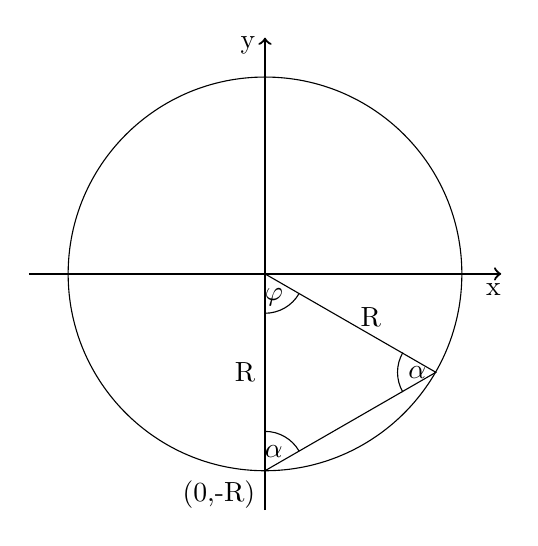
\begin{tikzpicture}[scale=1]
\draw (2.5,0) arc (0:360:2.5);
\draw[->,thick] (-3,0) -- (3,0);
\node[below] at (2.9,0) {x};
\draw[->,thick] (0,-3) -- (0,3);
\node[left] at (0,2.9) {y};
\node[left] at (0,-2.8) {(0,-R)};
\draw (0,-2.5) -- (2.17,-1.25) -- (0,0);
\node[right] at (-0.125,-2.25) {$\alpha$};
\draw (0,-2) arc (90:30:0.5);
\node[left] at (2.17,-1.25) {$\alpha$};
\draw (1.75, -1.5) arc (210:150:0.5);
\node[right] at (-0.125,-0.3) {$\varphi$};
\draw (0,-0.5) arc (270:330:0.5);
\node[left] at (0,-1.25) {R};
\node[right] at (1.09,-0.55) {R};
\end{tikzpicture}
\end{center}
\probend
\bigskip

% L134
\setAuthor{Siim Ainsaar}
\setRound{lõppvoor}
\setYear{2012}
\setNumber{G 5}
\setDifficulty{6}
\setTopic{Kinemaatika}

\prob{Rehvid}
\solu
\begin{wrapfigure}{r}{0.4\textwidth}
\includegraphics[width=\linewidth]{2012-v3g-05-r_joonis}
\end{wrapfigure}
Rattad tuleb pöörata suunda, mis ühtib nende liikumissuunaga. Ilmselt asub auto
pöörlemistelg tagarataste telgedega samal sirgel. Samas asub see optimaaljuhul
ka nii vasaku kui ka parema esiratta teljel. Seega otsitav nurk
\[
\beta =
\operatorname{arccot} \left( \frac{a \cot\alpha - b}{a} \right)
=
\operatorname{arccot} \left( \cot\alpha - \frac ba \right).
\]
\probend
\bigskip

% L135
\setAuthor{Jaan Kalda}
\setRound{lõppvoor}
\setYear{2014}
\setNumber{G 5}
\setDifficulty{6}
\setTopic{Kinemaatika}

\prob{Kammid}
\solu
Kui hall kamm liigub ühe pii võrra, on uus pilt identne esialgsega ning järelikult on tume laik liikunud ühe \enquote{lainepikkuse} võrra. 
Ühe laikude \enquote{lainepikkuse} kohta tuleb 7 halli kammi piide \enquote{lainepikkust}, seega liiguvad hallid laigud 7 korda kiiremini kui hall kamm: $v=\SI 7{cm/s}$.
\probend
\bigskip

% L136
\setAuthor{Mihkel Kree}
\setRound{lahtine}
\setYear{2014}
\setNumber{G 10}
\setDifficulty{8}
\setTopic{Kinemaatika}

\prob{Päikese pöörlemine}
\solu
Olgu Päikese pöörlemise joonkiirus ekvaatoril $v$. Kuna punktid A ja B lähenevad meile ja kaugenevad meist kiirusega $v$, siis mõõdetavad lainepikkused $\lambda_\text{A}$ ja $\lambda_\text{B}$ erinevad algsest lainepikkusest $\lambda_0$ Doppleri nihke tõttu. Punktist A näib kiirguvat lühem lainepikkus $\lambda_\text{A}=\lambda_0(1-v/c)$ ning punktist B pikem $\lambda_\text{B}=\lambda_0(1+v/c)$.

Kes Doppleri valemit peast ei tea, võib arutleda ka järgnevalt. Liikugu kiirguse allikas meie poole kiirusega $v$. Lainepikkusele $\lambda_0$ vastava laine sagedus on $f_0=\frac{c}{\lambda_0}$, järelikult võime mõelda, et lainehari kiiratakse iga intervalli $\tau = 1/f_0 = \lambda_0/c$ järel, mis vastab laine perioodile. Kiiratagu mingil hetkel esimene lainehari. Ühe perioodi jooksul liigub see kaugusele $x=c\tau$; allikas ise liigub aga selle aja jooksul meile lähemale $\Delta x = v\tau$ võrra ja kiirgab sealt järgmise laineharja. Niisiis tundub meile kui vaatlejale, et kahe laineharja vaheline kaugus ehk lainepikkus on 
\[
\lambda'=x-\Delta x=(c-v)\tau = \lambda_0(1-v/c).
\]

Punktidest A ja B mõõdetud lainepikkuste erinevus avaldub niisiis kui 
\[
\Delta\lambda = \lambda_\text{B}-\lambda_\text{A} = 2\lambda_0 v/c,
\]
kust saame lihtsalt avaldada joonkiiruse $v=c\Delta\lambda/2\lambda_0$ ning selle abil ka pöörlemisperioodi:
\[
T_\text{p}=\frac{2\pi r}{v}=\frac{4 \pi r \lambda_0}{c\Delta \lambda}=
\frac{4 \cdot 3.14 \cdot 7\cdot 10^8 \cdot 5.9 \cdot 10^{-7}}{3\cdot 10^8\cdot 7.8\cdot 10^{-12}}\,\text{s}\approx 26 \textit{T}_\mathrm{m}.
\]
Päike ei ole tahke keha, selle erinevad laiuskraadid pöörlevad erineva nurkkiirusega. Pooluselähedastel piirkondadel kulub ühe täispöörde tegemiseks umbes 34 päeva.
\probend
\bigskip

% L137
\setAuthor{Jaan Kalda}
\setRound{lõppvoor}
\setYear{2014}
\setNumber{G 9}
\setDifficulty{8}
\setTopic{Kinemaatika}

\prob{Traatrõngad}
\solu
Läheme süsteemi, mis pöörleb nurkkiirusega $\omega/2$; seal on näha, et lõikepunkt ei pöörle, vaid liigub radiaalselt.
Seega, laboratoorses süsteemis on selle nurkkiirus $\omega/2$; sellise nurkkiirusega pöörleb kõõl $AB$; et kesknurk on kahekordne piirdenurk, siis 
raadius $OB$ (kus $O$ on seisva rõnga keskpunkt) pöörleb nurkkiirusega $\omega$ ning järelikult on lõikepunkti kiirus samaselt võrdne $\omega R$-ga.
\probend
\bigskip

% L138
\setAuthor{Jaan Kalda}
\setRound{lahtine}
\setYear{2016}
\setNumber{G 9}
\setDifficulty{9}
\setTopic{Kinemaatika}

\prob{Anemomeeter}
\solu
Leviaegade suhtelised erinevused on väikesed, seega võime lugeda, et helikiirus on hulga suurem tuule kiirusest.
Vaatleme heli levikut õhuga seotud taustsüsteemis, kus sensorite suhtelise nihke $x$- ja $y$-telje sihilised komponendid ($s_x=u_x\frac a{c_s}$ ja 
$s_y=u_y\frac a{c_s}$) on samuti väikesed: $s_x, s_y\ll a$; $u_x$ ja $u_y$ tähistavad tuule kiiruse komponente ning $c_s$ - heli kiirust.
Rangelt võttes pidanuksid siin valemeis olema täpsed lennuajad $t_A$, $t_B$ ja $t_C$, kuid nihked ise on väikesed ning leviaegade 
väikeste vahede tõttu tuleb viga juba tühiselt väike. Niisiis saame leviaegade jaoks avaldised:
\begin{align*}
t_A&=\frac 1{c_s}\left(a+u_y\frac a{c_s}\right),\\
t_B&=\frac 1{c_s}\left(a+u_x\frac a{c_s}\right)\;\; \mbox{ja}\\
t_C&=\frac 1{c_s}\left(a-u_x\frac a{c_s}\right),
\end{align*}
millest $ \frac a{c_s}=\frac 12(t_B+t_C)$, $$u_x=\frac {c_s^2}a\left[t_B-\frac 12(t_B+t_C)\right]=c_s\frac{t_B-t_C}{t_B+t_C}=2a\frac{t_B-t_C}{(t_B+t_C)^2}\approx \SI{6.1}{m/s}$$
ning 
$$u_y=\frac {c_s^2}a\left[t_A-\frac 12(t_B+t_C)\right]=2a\frac{2t_A-t_B-t_C}{(t_B+t_C)^2}\approx \SI{7.1}{m/s}.$$
Seega on tuule kiirus $u=\sqrt{u_x^2+u_y^2}\approx \SI{9.4}{m/s}$.
\probend
\bigskip

% L139
\setAuthor{Jaan Kalda}
\setRound{lõppvoor}
\setYear{2016}
\setNumber{G 9}
\setDifficulty{9}
\setTopic{Kinemaatika}

\prob{Kaater}
\solu
Vaatleme kaatri liikumist õhu suhtes: alguses $l_1=t_1v_1=\SI{2700}m$ itta, siis $l_2=t_2v_2=\SI{900}m$ kagusse
ning lõpuks $l_3=t_3v_3=\SI{450}m$ edelasse. Kokkuvõttes nihkuti lõunasuunas 
\[
L_S=\frac{l_2+l_3}{\sqrt 2}\approx \SI{955}m
\]
ning idasuunas
\[
L_E=l_1+\frac{l_2-l_3}{\sqrt 2}\approx \SI{3018}m,
\]
maa suhtes aga nihkuti $l$ võrra lõunasse. Seetõttu pidi õhk liikuma $L_E$ võrra läände ning $l-L_S$ võrra lõunasse. Siit saame tuule tugevuseks 
$$v_t=\frac{\sqrt{L_E^2+(l-L_S)^2}}{t_1+t_2+t_3}\approx \SI{11.9}{m/s}\approx \SI{12}{m/s}.$$
\probend
\bigskip

% L140
\setAuthor{Kristian Kuppart}
\setRound{lahtine}
\setYear{2013}
\setNumber{G 2}
\setDifficulty{3}
\setTopic{Magnetism}

\prob{Magnetpeegel}
\solu
Magenetvälja sattununa hakkab osake liikuma mööda ringjoone kaart, mille kõverusraadiuse saame leida, kui mõtleme, et ringliikumiseks vajaliku kesktõmbejõu annab Lorentzi jõud:
\[m\frac{v^2}{r}=qvB, \quad \text{millest} \quad r=\frac{mv}{qB}.\]
Kui langemisnurk $\alpha$ on piisavalt väike, läbib osake magnetvälja riba. Kui hakkame $\alpha$-t
suurendama, saabub olukord, kus ühel hetkel osake enam magnetvälja riba ei läbi, vaid ``peegeldub'' tagasi. Sellel piirjuhul (vt joonist):

\[r\sin\alpha_\text{max}+d=r, \quad \text{millest} \quad \alpha_\text{max}=\sin^{-1}\left(1-\frac{d}{r}\right).\]

\begin{center}
\includegraphics[width=0.9\textwidth]{2013-lahg-02-magPeegLah.pdf}
\end{center}
\probend
\bigskip

% L141
\setAuthor{Andreas Valdmann}
\setRound{lahtine}
\setYear{2013}
\setNumber{G 5}
\setDifficulty{4}
\setTopic{Magnetism}

\prob{Generaator}
\solu
\osa Elektrivool generaatori mähises (juhtmekontuuris) tekib elektromagnetilise induktsiooni toimel ning seda protsessi kirjeldab Faraday seadus
$$
\varepsilon = -\frac{\Delta\Phi}{\Delta t},
$$
kus $\varepsilon$ on voltides mõõdetav elektromotoorjõu suurus ning $\Delta\Phi$ on juhtmekontuuri läbiva magnetvoo muutus, mis toimub ajavahemiku $\Delta t$ jooksul. Magnetvoo suurus $\Phi$ sõltub mähise asendist generaatori magnetite suhtes. Mähise pöörlemissageduse suurendamisel 2 korda kulub magnetvoo muutmiseks $\Delta\Phi$ võrra 2 korda vähem aega ja seetõttu suureneb elektromotoorjõud 2 korda. Kuna generaatoris kaod puuduvad, siis võib tema sisetakistuse lugeda nulliks ning antud juhul on generaatori klemmipinge $U$ alati võrdne tema elektromotoorjõuga. Lambis eralduv võimsus avaldub kujul
$$
P = UI = \frac{U^2}{R},
$$
Kus $I$ on voolutugevus lambis ning $R$ on lambi takistus. Kuna viimane ei muutu, siis järelikult suureneb pinge kahekordsel suurendamisel võimsus $2^2=4$ korda. Seega $P_1=4P_0$.\\
\osa Jõumomendi avaldamise näitlikustamiseks kujutame ette, et generaatorit pööratakse vändaga, mille õla pikkus on $l$ ning mille otsale avaldatakse tangentsiaalselt jõudu $F$. Pöördemoment $M$ avaldub kui $M=Fl$. Kadude puudumisel on generaatori pööramise võimsus võrdne lambil eralduva võimsusega. Definitsioonist teame, et mehaaniline võimsus on töö tegemise kiirus ehk
$$
P = \frac{A}{\Delta t},
$$
kus $A$ on ajavahemiku $\Delta t$ jooksul tehtud töö, mis avaldub omakorda jõu ja nihke korrutisena $A=F \Delta s$. Nihe $\Delta s$ kujutab antud juhul vända otspunkti tangentsiaalset liikumist, milleks kulus ajavahemik $\Delta t$. Vända otspunkti nihe avaldub kui $\Delta s=\Delta\phi l$, kus $\Delta\phi$ on nihkele vastav pöördenurk. Niisiis saame avaldada mehaanilise võimsuse:
$$
P = F \frac{\Delta s}{\Delta t} =Fl \frac{\Delta\phi}{\Delta t}.
$$
Paneme tähele, et avaldises esinev $\Delta\phi / \Delta t$ on vända pöörlemise nurkkiirus $\omega$. Kõrvutades tulemust varem leitud jõumomendi avaldisega, saame lihtsa seose $P=M\omega$. Esialgsel juhul oli generaatorit pöörav jõumoment seega
$M_0 = P_0/\omega_0$. Kuna $\omega_1=2\omega_0$ ja $P_1=4P_0$, siis oli pöördemoment pärast sageduse suurendamist
\[
M_1 = P_1/\omega_1=2P_0/\omega_0.
\]
\probend
\bigskip

% L142
\setAuthor{Eero Vaher}
\setRound{lahtine}
\setYear{2013}
\setNumber{G 6}
\setDifficulty{5}
\setTopic{Magnetism}

\prob{Tiirlev kuulike}
\solu
Olgu positiivse laenguga kuulikese laeng $Q$. Kuulikesele mõjuks kirjeldatud magnetväljas Lorentzi jõud suurusega $F_L=QvB$. See jõud oleks kuulikesele mõjuvaks kesktõmbejõuks $F_k=\frac{mv^2}{r}$. Saame $QvB=\frac{mv^2}{r}$. Kaks isoleeritud võrdse massiga kuulikest tiirlevad ümber ühise masskeskme, seega on nende omavaheline kaugus $d=2r$. Kuulikesi ringorbiidil hoidvaks kesktõmbejõuks on kuloniline jõud suurusega 
\[
F_C=\frac{kqQ}{d^2}=\frac{kqQ}{4r^2}.
\]
Kuna teineteise ümber tiirlevad laengud peavad olema vastasmärgilised, siis $|F_C|=-F_C$. Võrdsustades kesktõmbejõu ning kulonilise jõu suuruse, saame
\[
\frac{mv^2}{r}=-\frac{kqQ}{4r^2}
\]
ehk
\[
QvB=-\frac{kqQ}{4r^2}.
\]
Lõpptulemuseks saame 
\[
q=-\frac{4vBr^2}{k}.
\]
\probend
\bigskip

% L143
\setAuthor{Kristian Kuppart}
\setRound{piirkonnavoor}
\setYear{2018}
\setNumber{G 10}
\setDifficulty{6}
\setTopic{Magnetism}

\prob{Tsüklotron}
\solu
Osakesed hakkavad tsüklotronis liikuma päripäeva mööda järjest suureneva raadiusega poolringjooni. Osakese trajektoori raadius avaldub kui $r=mv/qB$, kus $v$ on osakese kiirus. Osake väljub tsüklotronist, kui tema trajektoori raadius kasvab sama suureks tsüklotroni raadiusega $R$, sel juhul tema kiirus $v=qBR/m$. Ühe täisringi jooksul saab osake elektriväljalt kineetilise energia $\varepsilon_k=2qEd$, kuna osake läbib selle aja jooksul riba 2 korda. Seega on osakese kiirus tsüklotronist väljumisel
\[\frac{mv^2}{2}=2qEdn, \qquad v^2=\frac{4qEdn}{m}.\]
Avaldades neist võrranditest $n$, saame $\displaystyle n=\frac{qB^2R^2}{4mEd}$.
\probend
\bigskip

% L144
\setAuthor{Kristian Kuppart}
\setRound{piirkonnavoor}
\setYear{2013}
\setNumber{G 10}
\setDifficulty{7}
\setTopic{Magnetism}

\prob{Mass-spektromeeter}
\solu
Potentsiaalide vahes $U$ saab kiirendatud laetud osake kineetilise
energia
\[
\frac{mv^{2}}{2}=qU,
\]
siit avaldame osakese kiiruse:
\[
v=\sqrt{\frac{2qU}{m}}.
\]
Kuna magnetväli on kiirusega risti, hakkab laetud osake 
magnetvälja jõudes liikuma seal mööda ringjoone kaart, kus ringjoone raadius
$R=\frac{mv}{qB}$. Selleks ajaks, kui osake jõuab detektorini,
on ta läbinud pool ringjoonest. Olgu $m_{2}$ raskema isotoobi
mass ja $m_{1}$ kergema isotoobi mass. Sel juhul 
\[ 
2\left(\frac{m_{1}v_{1}}{qB}-\frac{m_{2}v_{2}}{qB}\right)=d, 
\]
ehk
\[ 
m_{2}v_{2}=\frac{qBd}{2}+m_{1}v_{1 }.
\]
Arvestades, et $v_{1}=\sqrt{\frac{2eU}{m_{1}}}$ ja $v_{2}=\sqrt{\frac{2eU}{m_{2}}}$,
kus $e$ on elementaarlaeng, saame eelmise võrrandi ümber kirjutada kui
\[ \sqrt{m_{2}}=\sqrt{m_{1}}+\frac{Bd}{2}\sqrt{\frac{e}{2U}}. \]
Võttes arvesse, et $m_{2}=\frac{\mu_{2}}{N_{A}}$ ja $m_{1}=\frac{\mu_{1}}{N_{A}}$,
kus $N_{A}$ on Avogadro arv, saame:
\[ \mu_{2}=N_{A}\left(\sqrt{\frac{\mu_{1}}{N_{A}}}+\frac{Bd}{2}\sqrt{\frac{e}{2U}}\right)^{2}.\]
\probend
\bigskip

% L145
\setAuthor{Jaan Kalda}
\setRound{piirkonnavoor}
\setYear{2015}
\setNumber{G 9}
\setDifficulty{8}
\setTopic{Magnetism}

\prob{Magnetväli}
\solu
\begin{center}
\includegraphics[width=0.7\textwidth]{2015-v2g-09-magnetvalilah}
\end{center}
Laeng sooritab magnetväljas ringliikumist, vt joonis;
ringi raadiuse leiame Newtoni II seadusest $Bqv=mv^2/R$, millest
$R=\frac{mv}{qB}$. Enne ja pärast ringliikumist on trajektooriks sirge, kusjuures üleminek ringjooneks on ilma murdepunktita, st sirgjooned on ringile puutujaks. Väikeste kiiruste korral, kui $R<a$, st $v<\frac{Bqa}{m}$, siis läheb osake otse tagasi,
st väljumisnurk $\varphi=\pi \SI{}{rad}=180^\circ$.

Väljudes on kiirusvektor risti ringi raadiusega, st $\angle OBD=\frac \pi 2$, mistõttu $\varphi=\angle COB$. Seega,
\[
\varphi=\arcsin \frac{BC}{BO}=\arcsin \frac{a}{R}=\arcsin \frac{qBa}{mv}.
\]
\probend
\bigskip

% L146
\setAuthor{Eero Vaher}
\setRound{lahtine}
\setYear{2015}
\setNumber{G 10}
\setDifficulty{9}
\setTopic{Magnetism}

\prob{Laetud pendel}
\solu
Kuulikesele mõjuvad raskusjõud $F_g$, niidi pinge $T$ ning Lorentzi jõud $F_L$. Kuulike püsib ringjoone kaarekujulisel trajektooril seni, kuni sellele mõjuvate jõudude projektsioonid niidi sihile rahuldavad võrrandit $T+F_L-F_g\cos\alpha=F_k$, kus $\alpha$ on niidi kõrvalekaldenurk tasakaaluasendist ning $F_k$ on ringjoone kaarel püsimiseks tarvilik kesktõmbejõud. Kuulikese ringjoone kaarekujulisest trajektoorist kõrvalekaldumisel ei saa niit olla pinges. Järelikult pole kuulikese trajektoor enam ringjoone kaar juhul $F_L>F_g\cos\alpha+F_k$. Olgu $v$ kuulikese kiirus nurga $\alpha$ korral, mille saame leida energia jäävusest 
\[
\frac{mv^2}{2}=-mg\Delta h,
\]
kus $\Delta h=l\cos\alpha-l+H$ on kuulikese kõrguse muut. Järelikult 
\[
v=\sqrt{2g\left(l\cos\alpha-l+H\right)}=\sqrt{2gl\left(\cos\alpha-\frac{1}{8}\right)}
\]
ning lahendamist vajav võrrand on $qBv=mg\cos\alpha+\frac{mv^2}{l}$ ehk 
\[
qB\sqrt{2gl\left(\cos\alpha-\frac{1}{8}\right)}=mg\cos\alpha+2mg\left(\cos\alpha-\frac{1}{8}\right).
\]
Mõlemaid pooli ruutu võttes saame
\[
2q^2B^2gl\left(\cos\alpha-\frac{1}{8}\right)=m^2g^2\left(3\cos\alpha-\frac{1}{4}\right)^2.
\] 
Kuna $2q^2B^2l=\frac{3}{2}m^2g$, siis võime selle võrrandi viia kujule 
\[
\frac{3}{2}\cos\alpha-\frac{3}{16}=9\cos^2\alpha-\frac{3}{2}\cos\alpha+\frac{1}{16}.
\]
Saame ruutvõrrandi $9\cos^2\alpha-3\cos\alpha+\frac{1}{4}=0$ ehk $9\left(\cos\alpha-\frac{1}{6}\right)^2=0$. Kuna selle ruutvõrrandi kaks lahendit on võrdsed, siis kas $F_L\leq F_g\cos\alpha+F_k$ või $F_L\geq F_g\cos\alpha+F_k$ iga $\alpha$ korral. Vaadeldes juhtu $\cos\alpha=\frac{1}{8}$ näeme, et $F_L\leq F_g\cos\alpha+F_k$ ning järelikult on kuulikese trajektoor ringjoone kaar raadiusega $l$, mille otspunktide kõrgus tasakaaluasendist on $\frac{7}{8}l$.
\probend
\bigskip

% L147
\setAuthor{Jaan Kalda}
\setRound{lõppvoor}
\setYear{2017}
\setNumber{G 10}
\setDifficulty{10}
\setTopic{Magnetism}

\prob{Elektronid}
\solu
Maksimaalse $y$-telje sihilise läbimõõdu leidmiseks vaatleme osakesi, mis liiguvad $x-y$-tasandis. Sellisel juhul on elektroni trajektooriks ringjoon, sest magnetvälja poolt mõjuv jõud $F=evB$ on konstantse suurusega ja kiirusega kogu aeg risti. Raadiuse saame leida, pannes magnetvälja poolt mõjuva jõu võrduma kesktõmbejõuga:
$$\frac{mv^2}{R}=evB \hence R = \frac{mv}{Be}.$$
Kõik selles tasandis olevad elektronid liiguvad sama raadiusega ringjoonel ja eri nurkade all liikuva elektronide trajektoorid saab leida seda ringjoont lihtsalt pöörates ümber punkti O. Kõige kaugemale $y$-telje positiivses suunas jõuab elektron siis, kui ekraani tabades on ta algpunktist võimalikult kaugel ehk läbinud täpselt pool ringjoone kaart, vaata joonist:
\begin{center}
	\begin{tikzpicture}
	\def\aEl{1};
	\def\rEl{1.5};
	\coordinate (P1) at (-\aEl,{sqrt(4*\rEl*\rEl-\aEl*\aEl)});
	\coordinate (P2) at (-\aEl*0.5,{0.5*sqrt(4*\rEl*\rEl-\aEl*\aEl)});
	\node[label=below right:O, fill=black, circle,inner sep=1pt] at (0,0){};
	\path let \p1=(P1) in node [label=left:b] at (-\aEl, \y1/2){};
	\node[label=right:Q, fill=black, circle,inner sep=1pt] at (P2){};
	\node[label=below:a] at (-\aEl/2,0){};
	\node [label=above:$y$] at (-\aEl, 2.5*\rEl){};
	\draw[->] (-\aEl,-\rEl/2) -- (-\aEl, 2.5*\rEl);
	\draw (0,0) -- (P1);
	\draw (0,0) -- (-\aEl,0);
	%\draw (0,0) arc ({-90+asin(\aEl/(2*\rEl))}:{360-(-90+asin(\aEl/(2*\rEl)))}:\rEl);
	\draw (0,0) arc ({-90+asin(\aEl/(2*\rEl))}:90+asin(\aEl/(2*\rEl)):\rEl);
	%\draw [red](P1) ++ (-90:0.4) arc (-90:-90+\angKatus:0.4);
	\end{tikzpicture}
\end{center}

Kuna ekraan on kaugusel $a$ elektronide allikast, siis Pythagorase teoreemi järgi saame laigu maksimaalseks $y$ väärtuseks $$b=\sqrt{4R^2-a^2} = \sqrt{4\left(\frac{mv}{Be}\right)^2-a^2}.$$
Siit näeme, et väiksemale $R$-ile vastab väiksem läbimõõt ja maksimaalne $y$-telje sihiline läbimõõt on tõesti siis, kui osake liigub $x-y$-tasandis, nagu ka alguses väitsime.

Ringjoone kaart ümber punkti $O$ pöörates näeme, et minimaalne $y$-suunalise väärtuse korral on ringjoon ekraanile puutujaks, vaata joonist:
\begin{center}
	\begin{tikzpicture}
	\def\aEl{1};
	\def\rEl{1.5};
	\coordinate (P1) at (\rEl-\aEl,{-sqrt(\rEl*\rEl-(\rEl-\aEl)*(\rEl-\aEl))});
	\node[label=above right:O, fill=black, circle,inner sep=1pt] at (0,0){};
	\node[label=below right:Q, fill=black, circle,inner sep=1pt] at (P1){};
	\path let \p1=(P1) in node[label=below:T, fill=black, circle,inner sep=1pt] at (0,\y1){};
	%\path let \p1=(P1) in node [label=left:b] at (-\aEl, \y1/2){};
	\node[label=above:a] at (-\aEl/2,0){};
	\node [label=above:$y$] at (-\aEl, 0.5*\rEl){};
	\draw[->] (-\aEl,-2*\rEl) -- (-\aEl, 0.5*\rEl);
	\draw (0,0) -- (P1);
	\draw (P1) -- ($(P1)-(1.0*\rEl,0)$);
	\draw (0,0) -- (-\aEl,0);
	%\draw (0,0) arc ({180-acos((\rEl-\aEl)/\rEl)}:{360}:\rEl);
	\draw (P1) ++ (-180:\rEl) arc (180:-180:\rEl);
	%\draw (0,0) arc ({180-acos((\rEl-\aEl)/\rEl)}:180:\rEl);
	%\draw [red](P1) ++ (-90:0.4) arc (-90:-90+\angKatus:0.4);
	\end{tikzpicture}
\end{center}
Kuna lõigu QT pikkus on $R-a$, siis lõigu OQ $y$-suunalise komponendi saab leida Pythagorase teoreemi abil
$$y\idx{min}=-\sqrt{R^2-(R-a)^2} = -\sqrt{2aR-a^2}=-\sqrt{\frac{2amv}{Be}-a^2}.$$
Seega laigu $y$-suunaline läbimõõt on
$$L=\sqrt{\frac{2amv}{Be}-a^2} + \sqrt{4\left(\frac{mv}{Be}\right)^2-a^2}.$$

Selle laigu peal on heledus kõige suurem maksimaalse $y$ väärtuse korral, sest see vastab elektroni $y$-telje sihilise kõrvalekalde $\Delta_y$ ekstreemumile. 
Kui tähistame elektroni stardinurga $\alpha$ abil, siis 
$$\frac{\D \Delta_y}{\D \alpha}=0,$$
st väikeses stardinurga vahemikus $\Delta\alpha$ saabuvad kõik elektronid peaaegu täpselt samasse sihtpunkti.

Leiame $z$-telje sihilise läbimõõdu tasandis $y=0$. Kõige kaugemale $z$-teljel jõuavad need on osakesed, mille 
heeliksikujuline trajektoor puudutab tasandit $x=-a$ (``ülaltvaates'' $x-y$-tasandile puudutab ringjoonekujuline trajektoor raadiusega $r=\frac a2$ 
joont $x=-a$) ja mis stardivad $y-z$-tasandis, st algkiirusega, mille $x$-projektsioon $v_x=0$.
Edasi leiame $$\frac a2=\frac {mv_y}{Be}\hence v_y=\frac{aBe}{2m}\hence v_z=\sqrt{v^2-\left(\frac{aBe}{2m}\right)^2}.$$
Sellise algkiirusega elektronide teekond kestab pool tsüklotronperioodist. Perioodi saab leida seosest
\[
T=\frac{2\pi R}{v} = \frac{2\pi m}{Be}.
\]
Pool perioodi on seega
\[
t=\frac{T}{2}=\frac{\pi m}{Be}
\]
ning laigu $z$-telje sihiliseks 
mõõtmeks saame
$$2\cdot tv_z=\pi\sqrt{\left(\frac{2mv}{Be}\right)^2-a^2}.$$
\probend
\bigskip

% L148
\setAuthor{Taavi Pungas}
\setRound{piirkonnavoor}
\setYear{2014}
\setNumber{G 6}
\setDifficulty{4}
\setTopic{Staatika}

\prob{Rõngas}
\solu
Et süsteem oleks tasakaalus, peab mutter asuma täpselt nööri kinnituspunkti all. Teiseks: maksimaalse mutri kõrguse korral on rõnga kaldenurk mutri asukohas $\alpha$, kus $\tan \alpha = \mu$ - siis on mutter täpselt libisemise piiril. Sel juhul on ka mutrini tõmmatud raadiuse ja vertikaali vahel nurk $\alpha$. Tekkinud kolmnurgast näeme, et
\[
h=L+2R\cos \alpha = L+ \frac{2R}{\sqrt{1+\mu^2}}.
\]
\probend
\bigskip

% L149
\setAuthor{Mihkel Rähn}
\setRound{piirkonnavoor}
\setYear{2015}
\setNumber{G 7}
\setDifficulty{5}
\setTopic{Staatika}

\prob{Poldilõikur}
\solu
Jõu ülekandmine toimub kangi põhimõttel, kus jõumoment pöördtelje suhtes summaarselt on võrdne nulliga. Käepideme korral
\[ \SI{600}{mm}\cdot\SI{90}{N}-\SI{100}{mm}\cdot F_k = 0 \quad\Rightarrow\quad F_k = \SI{540}{N}, \]
kus $F_k$ on käepidemetelt lõiketeradele mõjuv jõud. Analoogselt lõiketerade korral
\[ \SI{160}{mm}\cdot F_k - \SI{80}{mm}\cdot F_l = 0 \quad\Rightarrow\quad F_l = 2F_k, \]
kus $F_l$ on lõikuri poolt poldile avaldatud jõud.\\
Nendest võrranditest saame leida lõiketeradele mõjuva jõu $F_l$
\[ F_l = \SI{1080}{N}.\]
\probend
\bigskip

% L150
\setAuthor{Mihkel Rähn}
\setRound{piirkonnavoor}
\setYear{2014}
\setNumber{G 7}
\setDifficulty{6}
\setTopic{Staatika}

\prob{Klotsid}
\solu
Ülemine klots ei libise, kui kiirendusest põhjustatud jõud ei ületa seisuhõõrdejõudu. Ülemise klotsi jaoks saab avaldada maksimaalse kiirenduse, mille korral klots veel ei libise, Newtoni teisest võrrandist $a_2=\mu_2g$. Kui ülemine klots ei libise, siis võib kahte klotsi käsitleda ühe kehana. Newtoni teine võrrand klotsisüsteemi kohta on 
\[
(m_1+m_2)a_{12} = -\mu_1 (m_1+m_2)g+F.
\]
Piirjuhul on kiirendused $a_{12}$ ja $a_2$ võrdsed. Asendades eelnevalt leitud kiirenduse $a_2$ võrrandisse liikmena $a_{12}$, saame
\[
F=(m_1+m_2)(\mu_1+\mu_2)g.
\]


Ülesannet võib lahendada ka koostades Newtoni teise võrrandi alumise klotsi kohta, võttes arvesse mõlemad hõõrdejõud.
\probend
\bigskip

% L151
\setAuthor{Mihkel Rähn}
\setRound{lõppvoor}
\setYear{2014}
\setNumber{G 6}
\setDifficulty{6}
\setTopic{Staatika}

\prob{Polüspast}
\solu
Hõõrdevaba ploki korral on pinge põhiköies jääv, muutub vaid selle suund. Hõõrdega ploki korral osa põhiköie pingest kandub plokile, kusjuures esmases lähenduses alla ja ülesse suunatud hõõrdejõud kompenseerivad üksteist. Tasakaalutingimuse rahuldamiseks peab ploki kinnituse pinge olema võrdne plokki läbiva põhiköie pingete summaga. Mittelibisevate sõlmede korral peab alla ja üles suunatud pingete vahel valitsema tasakaal. Lahendamist on mugav alustada, kui määrata päästjapoolseks tõmbejõuks $F$ ning alustada sellest otsast polüspasti läbimist. Hõõrdevabal juhul on jõuülekanne $\frac{5}{1}$, hõõrde korral $\frac{\num{2,4}}{1}$.

\begin{center}
\includegraphics[scale=0.25]{2014-v3g-06-PolyspastL1}
\includegraphics[scale=0.25]{2014-v3g-06-PolyspastL2}
\end{center}
\probend
\bigskip

% L152
\setAuthor{Andreas Valdmann}
\setRound{piirkonnavoor}
\setYear{2018}
\setNumber{G 9}
\setDifficulty{6}
\setTopic{Staatika}

\prob{Kelk}
\solu
Esiteks näeme, et kui Juku tõmbaks kelgunööri horisontaalselt, siis ei hakkaks kelk liikuma ükskõik kui suure tõmbejõu korral, sest Jukule mõjuv hõõrdejõud on väiksem kui kelgu liikumapanemiseks vajalik jõud:
\[
\mu_1 m_1 g < \mu_2 m_2 g.
\]
Esimesena hakkavad libisema hoopis Juku tallad.

Kui Juku tõmbab nööri teatud nurga all ülespoole, siis tekib nööris vertikaalne jõu komponent $F_{\mathrm{v}}$, mis tõstab kelku ülespoole ja surub Jukut allapoole. Seega mõjub Jukule tema libisemise piiril hõõrdejõud $F_{\mathrm{h}1} = \mu_1 \left(m_1 g + F_{\mathrm{v}}\right)$ ja kelgule tema libisemise piiril hõõrdejõud $F_{\mathrm{h}2} = \mu_2 \left(m_2 g - F_{\mathrm{v}}\right)$. Kuna küsiti minimaalset nurka, siis peab kelk olema libisemise piiri napilt ületanud ja Juku sellele napilt alla jääma ehk piirjuhul $F_{\mathrm{h}1} = F_{\mathrm{h}2} = F_{\mathrm{h}}$, kus $F_{\mathrm{h}}$ tähistab nööris tekkiva jõu horisontaalset komponenti.
Jõudude tasakaalu võrrandist
\begin{equation*}
\mu_1 \left(m_1 g + F_{\mathrm{v}}\right) = \mu_2 \left(m_2 g - F_{\mathrm{v}}\right)
\end{equation*}
saame avaldada nööris tekkiva jõu vertikaalse komponendi:
\begin{equation*}
\mu_1 m_1 g + \mu_1 F_{\mathrm{v}} = \mu_2 m_2 g - \mu_2 F_{\mathrm{v}},
\end{equation*}
\begin{equation*}
F_{\mathrm{v}} \left(\mu_1 + \mu_2\right) = g\left(\mu_2 m_2 - \mu_1 m_1\right),
\end{equation*}
\begin{equation*}
F_{\mathrm{v}} = g\frac{\mu_2 m_2 - \mu_1 m_1}{\mu_1 + \mu_2}.
\end{equation*}

Jõu horisontaalkomponendi leidmiseks asendame saadud tulemuse näiteks Jukule mõjuva hõõrdejõu võrrandisse
\begin{equation*}
F_{\mathrm{h}} = \mu_1 \left(m_1 g + g\frac{\mu_2 m_2 - \mu_1 m_1}{\mu_1 + \mu_2}\right)
\end{equation*}
ja avaldame:
\begin{align*}
F_{\mathrm{h}} &= g \mu_1 \frac{m_1 \left(\mu_1 + \mu_2\right) + \mu_2 m_2 - \mu_1 m_1}{\mu_1 + \mu_2} = \\
&= g \mu_1 \frac{\mu_2 m_1 + \mu_2 m_2}{\mu_1 + \mu_2} = g\mu_1\mu_2\frac{m_1+m_2}{\mu_1+\mu_2}.
\end{align*}

Nurk kelgunööri ja maapinna vahel on
\begin{equation*}
\alpha = \arctan\left(\frac{F_{\mathrm{v}}}{F_{\mathrm{h}}}\right) = \arctan\left(\frac{\mu_2 m_2 - \mu_1 m_1}{\mu_1 \mu_2 \left(m_1 + m_2\right)}\right) = \ang{21}.
\end{equation*}
\probend
\bigskip

% L153
\setAuthor{Mihkel Kree}
\setRound{lahtine}
\setYear{2013}
\setNumber{G 8}
\setDifficulty{7}
\setTopic{Staatika}

\prob{Niidirull}
\solu
Vaatleme silindrile mõjuvate jõumomentide tasakaalu telje suhtes, mis läbib toetuspunkti. Pinna toereaktsiooni ja hõõrdejõu vektorid läbivad toetuspunkti, mistõttu need jõumomenti ei tekita. Jõumomendi tekitavad kaks jõudu: silindri keskele rakendatud raskusjõud $mg$ ja nööri tõmbejõud $F$. Arvutades lihtsast kolmnurgast raskusjõu õla, saame jõumomendiks $\tau=mgr\sin\alpha$. Tasakaalu korral tekitab tõmbejõud $F$ sama suure, kuid vastassuunalise jõumomendi $-\tau$. Minimaalsele jõule peab vastama maksimaalne jõuõlg. Veendume, et kui jõud $F$ rakendada toetuspunktist diametraalselt vastas olevasse punkti, saame maksimaalse õla $2r$, millele vastab minimaalne tõmbejõud
\[F\idx{min}=\frac{\tau}{2r}=\frac{mg\sin\alpha}{2}.\]
\probend
\bigskip

% L154
\setAuthor{Andres Põldaru}
\setRound{lahtine}
\setYear{2014}
\setNumber{G 8}
\setDifficulty{7}
\setTopic{Staatika}

\prob{Jalgrattur}
\solu
Kuna tagumine ratas on õhku tõusmas, siis sellele jõude ei rakendu. Ainsad jalgrattale mõjuvad jõud on raskusjõud ning jõud esiratta ja maapinna kontaktpunktis. Kuna jalgratas liigub ühtlase kiirusega ning ei hakka pöörlema ega ümber kukkuma, peab jalgrattast ja ratturist koosnevale süsteemile mõjuvate jõudude summa ja ka jõumoment iga punkti suhtes olema null. Raskusjõu tugevus ja suund on teada. Teine jõud peab olema sama suur ja vastassuunaline, et raskusjõudu tasakaalustada. Lisaks peavad jõud paiknema ühel sirgel, et jalgratas koos ratturiga ei hakkaks pöörlema. Järelikult peab massikese olema esiratta ja maapinna kontaktpunkti kohal ning hõõrdejõu ja toereaktsiooni summa on vertikaalne. Lihtsast geomeetriast saame $\alpha=\arctan(\frac{d}{2h})$ ja $\mu\ge\frac{d}{2h}$.
\begin{center}
\includegraphics[width=0.6\textwidth]{2014-lahg-08-ratas}
\end{center}
\probend
\bigskip

% L155
\setAuthor{Stanislav Zavjalov}
\setRound{lahtine}
\setYear{2012}
\setNumber{G 9}
\setDifficulty{9}
\setTopic{Staatika}

\prob{Nöör rennis}
\solu
Olgu kogu nööri mass $m$. Vaatleme nööri paremat poolt. Nööri pinge vertikaalkomponent nööri ja plaadi kokkupuutepunktis, $T \sin \theta$, peab tasakaalustama õhus rippuva osa kaalu $\frac{f}{2}mg$. Nüüd vaatleme plaadil lebavat osa, selle mass on $\frac{1-f}{2}m$. Seega nii toereaktsioon kui ka maksimaalne hõõrdejõud (kuna $\mu = 1$) on $\frac{1-f}{2}mg \cos \theta$. Hõõrdejõud peab olema tasakaalus raskusjõu komponendiga piki nööri, $\frac{1-f}{2}mg \sin \theta$, ning pingega $T=\frac{f m g}{2 \sin \theta}$: $$\frac{f m g}{2 \sin \theta} + \frac{1-f}{2}mg \sin \theta = \frac{1-f}{2}mg \cos \theta.$$
Siit saame avaldada vastuse $$f = \frac{1-\tan \theta}{1+\tan \theta} \tan \theta. $$
\probend
\bigskip

% L156
\setAuthor{Jaan Kalda}
\setRound{lõppvoor}
\setYear{2017}
\setNumber{G 9}
\setDifficulty{9}
\setTopic{Staatika}

\prob{Katus}
\solu
Kahe traadi kontaktpunktis $A$ (vaata joonist allpool) mõjutavad traadid sümmeetria ja Newtoni III seaduse tõttu üksteist 
horisontaalsete vastassuunaliste jõududega; traadi ja silindri puutepunktis $B$ mõjub traadile rõhumisjõud, mis on traadiga risti ning seetõttu läbib selle jõu pikendus silindri telge $Q$. Raskusjõud on rakendatud traadi keskpunkti $C$. Et traat on tasakaalus ja talle mõjuvad kolmes punktis jõud, siis nende jõudude pikendused peavad lõikuma ühes punktis $O$ (vastasel korral mõjuks kahe jõu lõikumispunkti suhtes kolmas jõud traadile nullist erineva jõumomendiga ja traat hakkaks liikuma). Niisiis peavad punktist $A$ tõmmatud horisontaal, punktist $C$ tõmmatud vertikaal ning sirge $QB$ pikendus kõik lõikuma ühes punktis. Paneme tähele, et $\angle ACO=\alpha/2$ ja $\angle AOB=\alpha/2$, seetõttu
$$|AO|=|AC|\sin(\alpha/2)=(L/2)\sin(\alpha/2),$$ $$|AB|=|AO|\sin(\alpha/2)=(L/2)\sin^2(\alpha/2)$$ ning
$$R=|QB|=|AB|\tan(\alpha/2)=(L/2)\sin^3(\alpha/2)/\cos(\alpha/2).$$

\begin{center}
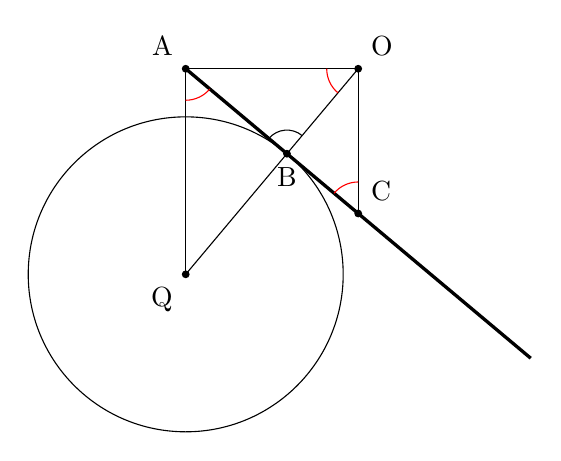
\begin{tikzpicture}
\usetikzlibrary{calc}
\def\angKatus{50};
\def\rKatus{2};
\coordinate (P1) at (0,{\rKatus/sin(\angKatus)});
\coordinate (P2) at ({\rKatus/sin(\angKatus)/tan(\angKatus)},{\rKatus/sin(\angKatus)});
\coordinate (P3) at ({\rKatus/sin(\angKatus)/tan(\angKatus)},{\rKatus/sin(\angKatus)-\rKatus/sin(\angKatus)/tan(\angKatus)/tan(\angKatus)});
%\fill (0,0) circle (0.05);
\node [label=below left:Q, fill=black, circle,inner sep=1pt] at (0,0){};
\draw (0,0) circle (\rKatus);
\node [label=above left:A, fill=black, circle,inner sep=1pt] at (P1){};
\node [label=above right:O, fill=black, circle,inner sep=1pt] at (P2){};
\node [label=above right:C, fill=black, circle,inner sep=1pt] at (P3){};
\node [label=below:B, fill=black, circle,inner sep=1pt] at (\angKatus:\rKatus){};
\draw [very thick](P1) -- (P3) -- ++($(P3)-(P1)$);
\draw (0,0) -- (P2);
\draw (0,0) -- (P1);
\draw (P1) -- (P2);
\draw (P3) -- (P2);
\draw [red](P1) ++ (-90:0.4) arc (-90:-90+\angKatus:0.4);
\draw [red](P3) ++ (90:0.4) arc (90:90+\angKatus:0.4);
\draw [red](P2) ++ (180:0.4) arc (180:180+\angKatus:0.4);
\draw (\angKatus:\rKatus) ++ (\angKatus:0.3) arc (\angKatus:90+\angKatus:0.3);
\end{tikzpicture}
\end{center}

Stabiilsuse analüüsi juures paneme tähele, et kui \enquote{katus} pöörleb tervikuna, siis massikese liigub mööda ringjoont ning küsimus on vaid selles, kas see on kõrgemal või madalamal kui silindri telg $Q$; viimasel juhul on massikese algasendis madalaimas positsioonis ning süsteem on stabiilne. Seega on stabiilsuse tingimuseks
$$|AQ|<|AC|\cos(\alpha/2).$$
Kui sellesse võrratusse asendame
$$|AQ|=|AB|/\cos(\alpha/2)=(L/2)\sin^2(\alpha/2)/\cos(\alpha/2)$$
ja $$|AC|\cos(\alpha/2)=(L/2)\cos(\alpha/2),$$ siis
saame, et $\sin^2(\alpha/2) < \cos^2(\alpha/2)$. Kuna katuse korral peab kehtima $0<\frac{\alpha}{2}<90$, siis nii $\sin$ kui $\cos$ on positiivsed ja võime võtta mõlemalt poolt ruutjuure. Saame tingimuse $\sin(\alpha/2) < \cos(\alpha/2)$, mis kehtib kui $\alpha<\pi/2$. Paneme tähele, et viimast tingimust võib esitada erinevatel viisidel, kasutades $R$, $L$ ja $\alpha$ vahelist seost.
\probend
\bigskip

% L157
\setAuthor{Jaan Kalda}
\setRound{lõppvoor}
\setYear{2015}
\setNumber{G 9}
\setDifficulty{10}
\setTopic{Staatika}

\prob{Niidiga hantel}
\solu
Pulgale mõjuvad kolm jõudu. Jõumomentide tasakaalu tõttu peavad nende jõudude rakendussirged lõikuma ühes punktis, olgu see punkt $C$. Olgu niidi rakenduspunkt $N$ ja pulga otspunktid $A$ ning $B$, vt joonis. Kuna enne klotsi $A$ paigalt nihkumist pöörleb pulk ümber selle, siis punkti $B$ kiirusvektor on risti $AB$-ga, sama kehtib puntki $B$ rakendatud hõõrdejõu vektori jaoks; sestap $\angle ABC=\frac{\pi}{2}$. Et nihkuma hakkamise hetkel on hõõrdejõud võrdsed, siis jõudude kolmnurk $\vec F_1+\vec F_2=\vec T$ on võrdhaarne, järelikult on võrdhaarne ka jõudude kolmnurgaga sarnane kolmnurk $CBE$ (sirge $BE$ on tõmmatud paralleelsena $\vec T$-ga ja $E$ asub $\vec F_1$ rakendussirgel, vt joonis).
Olgu $|CB|=b$; siis ka $|CE|=b$. Seetõttu kolmnurkade $ANC$ ja $ABE$ sarnasuse põhjal $|AC|=3b$. Pythagorase
teoreemist kolmnurga $ABC$ jaoks $9b^2=b^2+16a^2$, st $b=\sqrt 2a$. Seetõttu otsitav nurk 
\[
\angle BNC=\arctan \frac ba =\arctan \sqrt 2\approx\SI{0.96}{rad}\approx 55^\circ.
\]
\begin{center}
\includegraphics[width=0.7\textwidth]{2015-v3g-09-pulk_lah}
\end{center}
\probend
\bigskip

% L158
\setAuthor{Eero Vaher}
\setRound{piirkonnavoor}
\setYear{2014}
\setNumber{G 3}
\setDifficulty{2}
\setTopic{Taevamehaanika}

\prob{Maa pöörlemisperiood}
\solu
Päikese näivat liikumist taevas põhjustavad nii Maa pöörlemine kui ka tiirlemine. Maa tiirlemise tõttu erineb Maa täispöörete arv aastas ühe võrra keskmiste päikeseööpäevade arvust. Kuna Maa tiirlemise suund ühtib Maa pöörlemise suunaga, teeb Maa ühe aasta jooksul ühe täispöörde rohkem. Seega on Maa pöörlemisperioodiks
\[
P=\frac{\num{365,256}}{\num{366,256}} \cdot \SI{86400}{\second}=\SI{86164}{\second}=\SI{23}{\hour} \SI{56}{\minute} \SI{4}{\second}.
\]

\vspace{0.5\baselineskip}
\emph{Alternatiivne lahendus}\\
Päike teeb täistiiru taevas sagedusega $f_k=\frac{1}{\SI{86400}{\second}}$. Maa tiirlemise sagedus on $f_t=\frac{1}{\num{365,256}\cdot86400\text{s}}$. Kuna Maa pöörlemis- ja tiirlemissuunad ühtivad, siis kehtib võrrand $f_k=f_p-f_t$, kus $f_p$ on Maa pöörlemise sagedus. Siit saame avaldada Maa pöörlemisperioodi 
\[
P=\frac{1}{f_p}=\frac{1}{f_k+f_t}=\SI{86164}{\second}=\SI{23}{\hour} \SI{56}{\minute} \SI{4}{\second}.
\]

\emph{Märkused.}

\vspace{-5pt}
\begin{itemize}[noitemsep, leftmargin=*]
\item Nimetuse keskmine päikeseööpäev tingib asjaolu, et Maa elliptilise orbiidi tõttu on Päikese näiv nurkkiirus taevas veidi muutlik.
\item Maa tiirlemisperioodi nimetatakse ka sideeriliseks aastaks. 
\item Enamasti mõistetakse aastana troopilist, mitte sideerilist aastat, mis on defineeritud pööripäevade kordumise põhjal. Troopilise ning sideerilise aasta erinemise põhjustab Maa telje pretsessioon. Igapäevaelus ei ole olulised mitte Maa pöörlemine ning tiirlemine vaid hoopis Päikese ööpäevane liikumine taevas ning aastaaegade kordumine, mistõttu laialdaselt kasutatavad ööpäeva ning aasta mõisted erinevadki Maa pöörlemis- ning tiirlemisperioodidest. 
\end{itemize}
\probend
\bigskip

% L159
\setAuthor{Mihkel Pajusalu}
\setRound{lahtine}
\setYear{2014}
\setNumber{G 3}
\setDifficulty{3}
\setTopic{Taevamehaanika}

\prob{Orbiit}
\solu
Selles ülesandes kasutame lähendust, et väikese massiga (olgu selleks $m$) punktmass Kuu tiirleb ümber suure punktmassi Maa. Paneme tähele, et Kuu gravitatsioonilise potentsiaalse energia ja kineetilise energia summa on jääv.
$$
\frac{mv_1^2}{2}-G\frac{Mm}{r_1}=\frac{mv_2^2}{2}-G\frac{Mm}{r_2}.
$$
Samuti on kõigil orbiitidel liikuvatel kehadel muutumatu impulsimoment. Kuna orbiidid on ellipsid, siis suurimal ja vähimal kaugusel Maast on Kuu orbitaalkiirus risti Kuud Maaga ühendava sirgega. Seega saab kirjutada impulsimomendi jäävuse seaduse suurima ja vähima kauguse jaoks kujul
$$
mv_1r_1=mv_2r_2.
$$
Kuu mass taandub mõlemast jäävusseadusest välja. Saame süsteemi
$$
\begin{array}{c} 
\frac{v_1^2}{2}-G\frac{M}{r_1}=\frac{v_2^2}{2}-G\frac{M}{r_2}.\\
v_1r_1=v_2r_2.
\end{array}
$$
Süsteemi lahenditeks on $r_2=r_1$, mis ei vasta elliptilisele orbiidile, ja $$r_2=\frac{1}{\frac{2GM}{r_1^2v_1^2}-\frac{1}{r_1}}\approx\SI{430000}{km}.$$
\probend
\bigskip

% L160
\setAuthor{Eero Vaher}
\setRound{piirkonnavoor}
\setYear{2013}
\setNumber{G 6}
\setDifficulty{4}
\setTopic{Taevamehaanika}

\prob{Päikese tihedus}
\solu
Päikese raadius on $r=R\sin\alpha/2$ ja ruumala $V=4\pi r^3/3$.
Maa joonkiirus oma orbiidil ümber Päikese on $v=\frac{2\pi R}{T}$. Et Maa püsiks oma orbiidil, peab sellele mõjuma kesktõmbejõud $F=\frac{mv^2}{R}$, kus $m$ on Maa mass. See kesktõmbejõud on teadagi Maa ja Päikese vaheline gravitatsioonijõud $G\frac{mM}{R^2}$, kus $M$ on Päikese mass, seega
\[
\frac{mv^2}{R}=G\frac{mM}{R^2}.
\]
Saame
\[
M=\frac{Rv^2}{G}.
\]
Päikese tihedus avaldub seosest $\varrho=\frac{M}{V}$, $$\varrho=\frac{Rv^2}{G} \frac{3}{4\pi r^3}=\frac{24 \pi R^3}{G T^2 \sin^3 \alpha}=\SI{1,4e3}{kg/m^3}.$$
\probend
\bigskip

% L161
\setAuthor{Eero Vaher}
\setRound{piirkonnavoor}
\setYear{2018}
\setNumber{G 6}
\setDifficulty{4}
\setTopic{Taevamehaanika}

\prob{Ühendatud satelliidid}
\solu
Trossi puudumisel peab satelliidile mõjuv kesktõmbejõud olema võrdne sellele mõjuva raskusjõuga. Esimese satelliidi jaoks
\[
\frac{{mv'_1}^2}{R_1}=G\frac{Mm}{R_1^2},
\]
millest järeldub
\[
v'_1=\sqrt{\frac{GM}{R_1}}
\]
ning analoogiliselt
\[
v'_2=\sqrt{\frac{GM}{R_2}}.
\]

Kuna satelliidid on trossiga ühendatud, siis seesmisele satelliidile mõjuv kesktõmbejõud peab olema sellele mõjuva raskusjõu ning trossi pinge vahe ning välimisele satelliidile mõjuv kesktõmbejõud peab olema sellele mõjuva raskusjõu ning trossi pinge summa. Niisiis
$$\begin{cases}
\frac{mv_1^2}{R_1}=G\frac{Mm}{R_1^2}-T,\\
\frac{mv_2^2}{R_2}=G\frac{Mm}{R_2^2}+T.
\end{cases}$$ 
Kuna $v_1=2\pi R_1/P$ ning $v_2=2\pi R_2/P$, siis saame kirjutada
$$\frac{4\pi^2}{P^2}\left(R_1+R_2\right)=GM\frac{R_2^2+R_1^2}{R_1^2R_2^2}.$$
Tehes asenduse $R_2=2R_1$, saame
\[
\frac{2\pi R_1}{P}=\sqrt{\frac{5GM}{12R_1}},
\]
ning asendusest $R_1=\frac{R_2}{2}$ järeldub
\[
\frac{2\pi R_2}{P}=\sqrt{\frac{10GM}{3R_2}}.
\]
Sisemine satelliit tiirleb niisiis trossi tõttu $\sqrt{12/5}$ korda väiksema ning välimine $\sqrt{10/3}$ korda suurema joonkiirusega.
\probend
\bigskip

% L162
\setAuthor{Eero Vaher}
\setRound{lõppvoor}
\setYear{2013}
\setNumber{G 5}
\setDifficulty{5}
\setTopic{Taevamehaanika}

\prob{Satelliit}
\solu
Satelliidile orbiidil mõjuv kesktõmbejõud on Maa poolt satelliidile avaldatav gravitatsioonijõud. Saame $$\frac{mv^2}{R}=G\frac{Mm}{R^2},$$kus $m$ on satelliidi mass ja $R$ orbiidi raadius. Kuna geostatsionaarne satelliit Maa suhtes ei liigu, peab selle tiirlemisperiood olema samuti 24 h. Saame $v=\frac{2\pi R}{t}$. Neist võrranditest saame $$4\pi^2 R^3=GM \Rightarrow R=\sqrt[3]{\frac{GMt^2}{4\pi^2}}=\SI{42400}{km}.$$ Maa keskpunkt, satelliit ning satelliidilt nähtava maa-ala serval asetsev suvaline punkt moodustavad täisnurkse kolmnurga, mille hüpotenuusiks on satelliidi orbiidi raadius ning üheks kaatetiks Maa raadius. Maa keskmes asuvaks nurgaks saame $\alpha=\arccos{\frac{r}{R}}$, kuid kuna meid huvitab satelliidilt nähtava ala läbimõõt, peame leidma nurga $2\alpha$. Sellele nurgale vastav kaare pikkus Maa pinnal on $d=2r\alpha$ (kui nurk on radiaanides). Lõppvastuseks saame 
$$d=2r\arccos \left(\frac{r}{\sqrt[3]{\frac{GMt^2}{4\pi^2}}}\right) =\SI{18000}{km}.$$
\probend
\bigskip

% L163
\setAuthor{Jaak Kikas}
\setRound{lahtine}
\setYear{2012}
\setNumber{G 1}
\setDifficulty{1}
\setTopic{Termodünaamika}

\prob{Vee jäätumine}
\solu
Vee jäätumisel eralduv soojushulk $m\idx{vesi} \lambda$ peab täpselt ära kuluma jää soojendamiseks:
\[
m\idx{vesi} \lambda = c\idx{jää} m\idx{jää} (t - t_0),
\]
kus $\lambda$ on jää sulamissoojus, $t=\SI{0}{\degreeCelsius}$ on jää lõpptemperatuur ja $t_0$ on otsitav jää algtemperatuur. Vee massi saame selle ruumalast, $m\idx{vesi} = \rho V\idx{vesi}$. Nendest kahest seosest saame avaldada
$$t_0 = t - \frac{\rho V\idx{vesi} \lambda}{c\idx{jää} m\idx{jää}} = -314 \,^{\circ}{\rm C}.$$
Ehk jää temperatuur peaks olema alla absoluutse nulli ja seega pole võimalik selle koguse jääkuubikutega kogu vett jääks muuta.
\probend
\bigskip

% L164
\setAuthor{Koit Timpmann}
\setRound{piirkonnavoor}
\setYear{2013}
\setNumber{G 2}
\setDifficulty{1}
\setTopic{Termodünaamika}

\prob{Veepudel}
\solu
Vesi jäätub temperatuuril \SI{0}{\degreeCelsius}. Vee jäätumisel eraldunud soojushulk läheb alajahtunud vee soojendamiseks jäätumistemperatuurile. Niisiis,
\[
cm\Delta t = \lambda m\idx{jää}
\]
ja
\[
m\idx{jää}=\frac{\SI{4200}{J / kg K} \cdot \SI{2}{kg} \cdot \SI{3}{\degreeCelsius}}{\SI{340000}{J / kg}}=\SI{74}{g}.
\]
\probend
\bigskip

% L165
\setAuthor{Ants Remm}
\setRound{lõppvoor}
\setYear{2012}
\setNumber{G 1}
\setDifficulty{2}
\setTopic{Termodünaamika}

\prob{Hõõrdkeevitus}
\solu
Hõõrdumisest tekkiv soojushulk
\[
Q = F_h \Delta s = F \mu \Delta s = \pi f D \Delta t.
\]
Teiselt poolt on torude soojendamiseks vaja minev soojushulk
\[
Q = 2 m c \Delta T = 2 \rho V c \Delta T,
\]
kus $m$ ja $V$ on ühe toruotsa soojeneva osa mass ja ruumala. Kuna toru seinad on diameetrist kordades õhemad, võib hinnata ruumalaks $V = \pi D d l$. Kokkuvõttes saame, et
\[
F \mu \pi f D \Delta t = 2 \pi D d l \rho c ( T_1 - T_0 ),
\]
\[
F = \frac{2 d l \rho c ( T_1 - T_0 )}{ \mu f \Delta t } \approx \SI{1200}{N}.
\]
\probend
\bigskip

% L166
\setAuthor{Erkki Tempel}
\setRound{piirkonnavoor}
\setYear{2015}
\setNumber{G 3}
\setDifficulty{2}
\setTopic{Termodünaamika}

\prob{Münt jääs}
\solu
Jäätükk koos mündiga hakkab uppuma siis, kui sellele mõjub raskusjõud on võrdne üleslükkejõuga. Tähistame uppumise hakkamise hetkel mündi ümber oleva jää massi $m$ ning ruumala $V$. Sellisel juhul mõjub jäätükile enne uppuma hakkamist raskusjõus $F_r=(m_m+m)g$ ning üleslükkejõud
\[ F_y=\rho_v g(V + V_m)=\rho_v g\left(\frac{m}{\rho_j} + \frac{m_m}{\rho_m}\right). \]

Kuna raskusjõud ja üleslükkejõud on uppumise hakkamise hetkel võrdsed, saame avaldada mündi ümber olnud jää massi $m$:
\[ m = \frac{\rho_j m_m(\rho_m - \rho_v)}{\rho_m(\rho_v - \rho_j)} = \SI{79,9}{g}. \]
Sulanud jää mass $m_s$ on seega
\[ m_s = m_j - m = m_j - \frac{\rho_j m_m(\rho_m - \rho_v)}{\rho_m(\rho_v - \rho_j)}. \]
Jää sulamiseks vajaminev energia $Q=\lambda m_s$ saadakse vee jahtumisel eraldunud energiast $Q=cm_v\Delta T$. Võrdsustades viimased avaldised ning avaldades $\Delta T$, saame
\[ \Delta T = \frac{\lambda m_s}{cm_v}. \]
Asendades siia sulanud jää massi $m_s$, saame temperatuuri muutuseks
\[ \Delta T \approx \SI{9,8}{\degreeCelsius}. \]
Kuna vee lõpptemperatuur pärast soojusvahetuse lakkamist on \SI{0}{\degreeCelsius}, peab vee algtemperatuur olema \SI{9,8}{\degreeCelsius}.
\probend
\bigskip

% L167
\setAuthor{Kaur Aare Saar}
\setRound{lõppvoor}
\setYear{2016}
\setNumber{G 1}
\setDifficulty{2}
\setTopic{Termodünaamika}

\prob{Soojusvaheti}
\solu
Nafta jahtumisel eraldunud soojus kulub vee soojendamiseks: $Q\idx{nafta} = Q\idx{vesi},$
\[ m_nc_n\Delta t_n = m_vc_v\Delta t_v \quad\Rightarrow \]
\[ \rho_nv_nc_n\Delta t_n = \rho_v v_vc_v\Delta t_v \quad\Rightarrow\quad \Delta t_v = \frac{\rho_nv_nc_n\Delta t_n}{\rho_vv_vc_v} \approx \SI{64}{\degreeCelsius}. \]
Seega väljub vesi soojusvahetist temperatuuril $T = \SI{64}{\degreeCelsius} + \SI{10}{\degreeCelsius} = \SI{74}{\degreeCelsius}$.
\probend
\bigskip

% L168
\setAuthor{Oleg Košik}
\setRound{piirkonnavoor}
\setYear{2012}
\setNumber{G 2}
\setDifficulty{3}
\setTopic{Termodünaamika}

\prob{Küttesüsteem}
\solu
Mingi ajavahemiku $\Delta t$ jooksul kaotab koolimaja väliskeskkonda soojust $Q_1=N\Delta t$, sama palju soojust peavad andma selle aja jooksul talle radiaatorid. Toru ristlõike pindala on $S=\frac{\pi D^2}{4}$. Aja $\Delta t$ jooksul küttesüsteemi siseneva ja ühtlasi sellest väljuva vee ruumala on seega $V=Sv\Delta t$, kus $v$ on otsitav veevoolu kiirus, ning mass $m=\rho V=\rho Sv\Delta t$. Radiaatorites eraldub soojushulk $Q_2=mc(t_0-t_1)$. Kuna $Q_1=Q_2$, saame võrrandi
\[
N\Delta t=\rho \frac{\pi D^2}{4}v\Delta t c (t_0-t_1),
\]
millest
\[
v=\frac{4N}{\pi D^2\rho c (t_0-t_1)}=0,15\;\hbox{m/s}.
\]
\probend
\bigskip

% L169
\setAuthor{Erkki Tempel}
\setRound{lahtine}
\setYear{2015}
\setNumber{G 4}
\setDifficulty{4}
\setTopic{Termodünaamika}

\prob{Veekeedukann}
\solu
Suurima kiiruse saavutab veeaur siis, kui vesi on kuumutatud keemistemperatuurini $T=\SI{100}{\degreeCelsius}=\SI{373}{K}$. Veekeedukannu tehtud töö $A=\gamma Nt$ läheb siis vee aurustamiseks ehk $A=Q=Lm$. Seega aja $t$ jooksul aurustunud vee mass on
\[
m=\frac{\gamma Nt}{L}
\]
ning ruumala
\[
V=\frac{\gamma NtRT}{Lp\mu}.
\]
Kuna veeaur pääseb välja avast pindalaga $S$, siis peab aja $t$ jooksul eraldanud veeaur läbima vahemaa $s=V/S$ ning veeauru väljumise kiiruseks saame
\[
v=\frac{s}{t}=\frac{\gamma NtRT}{Lp\mu S}.
\]
\probend
\bigskip

% L170
\setAuthor{Ardi Loot}
\setRound{piirkonnavoor}
\setYear{2018}
\setNumber{G 3}
\setDifficulty{4}
\setTopic{Termodünaamika}

\prob{Radiaator}
\solu
Leiame radiaatorit kirjeldava võrdeteguri $c_{r}$. Kuna radiaatori
väljundvõimus on võrdeline pealevoolu- ja tagasivoolutemperatuuride
keskmise ja toatemperatuuri vahega, siis
\[
P_{n}=c_{r}\left(\frac{T_{pn}+T_{tn}}{2}-T_{0n}\right)
\]
\noindent ja võrrandit lahendades saame
\[
c_{r}=\frac{2P_{n}}{T_{pn}+T_{tn}-2T_{0n}}=\SI{40}{W/K}.
\]
Nüüd paneme kirja võrrandisüsteemi radiaatori tegeliku võimuse ja
tagasivoolutemperatuuri jaoks
\[
\left\{ \begin{array}{c}
P=c_{r}\left(\frac{T_{p}+T_{t}}{2}-T_{0}\right)\\
P=\Gamma c_{v}\rho_{v}\left(T_{p}-T_{t}\right).
\end{array}\right.
\]
Esimene kirjeldab radiaatori väljundvõimust ja teine peale- ja tagasivoolutemperatuuride
vahest tingitud energiaülekannet. Lahendades võrrandid saame 
\begin{eqnarray*}
P & = & \frac{2\Gamma c_{v}\rho_{v}c_{r}\left(T_{p}-T_{0}\right)}{2\Gamma c_{v}\rho_{v}+c_{r}}\approx\SI{1.49}{kW}\\
T_{t} & = & \frac{2\Gamma T_{p}c_{v}\rho_{v}+c_{r}\left(2T_{0}-T_{p}\right)}{2\Gamma c_{v}\rho_{v}+c_{r}}\approx\SI{48.7}{\degreeCelsius}.
\end{eqnarray*}
Radiaatori maksimaalne võimsus on võimalik leida piirjuhuna, kui radiaatorit
läbiv vooluhulk $\Gamma$ kasvab väga suureks. Või veelgi lihtsamalt:
kui mõista, et sellisel juhul saab tagasivoolutemperatuur võrdseks
pealevoolutemperatuuriga ning maksimaalne võimsus avaldub
\[
P_{max}=c_{r}\left(T_{p}-T_{0}\right)\approx\SI{1.92}{kW}.
\]
\probend
\bigskip

% L171
\setAuthor{Kristian Kuppart}
\setRound{lahtine}
\setYear{2017}
\setNumber{G 6}
\setDifficulty{5}
\setTopic{Termodünaamika}

\prob{Kasvuhooneefekt}
\solu
Päikselt jõuab maale koguvõimsus $P_p=w_0 \left(1-\mu\right)\pi R^2$, kus $R$ on maa raadius. Kuna atmosfäär on maalt tuleva kiirguse jaoks läbimatu, peab tasakaalu korral atmosfäär väljapoole kiirgama selle sama võimsuse: $P_p=P_a$, kus $P_a$ on atmosfääri poolt väljapoole kiiratav võimsus. Maalt kiiratav võimsus avaldub kui $P_m=4 \pi R^2 \sigma T_m^4$, kus $T_m$ on maapinna temperatuur. Tasakaalu korral on see võrdne Päikeselt ja atmosfäärist tagasi kiirgunud võimsuste summaga:
\[P_m=P_p+P_a=2P_p.\]

Maakera temperatuur avaldub kui:

\[T_m=\sqrt[4]{\frac{w_0\left(1-\mu\right)}{2\sigma}}=\SI{303}{K}.\]
\probend
\bigskip

% L172
\setAuthor{Oleg Košik}
\setRound{lõppvoor}
\setYear{2013}
\setNumber{G 8}
\setDifficulty{7}
\setTopic{Termodünaamika}

\prob{Kauplus}
\solu
Soojusvahetus eesruumi ja õue vahel peab olema sama suur kui soojusvahetus eesruumi ja kaupluse vahel. Seega püsib päevasel ajal eesruumis temperatuur $T_4=\frac{T_0+T_1}{2}=\SI{12}{\degreeCelsius}$ kraadi ning eesruumi ehitusega vähenesid ukse lahtikäimisest tingitud soojuskaod 2 korda. See vähenemine oli $\Delta P=P_1-P_3=\SI{0,8}{kW}$, seega enne eesruumi ehitamist olid vastavad soojuskaod
\[
P_0=2\Delta P=\SI{1,6}{kW}.
\]
Päevasel ajal on temperatuuride vahe õuega $\Delta T_1=\SI{16}{\degreeCelsius}$ ning öisel ajal $\Delta T_2=\SI{20}{\degreeCelsius}$. Seega, kui päeval oleks kauplus kinni, siis kaupluse radiaatorid peaks töötama võimsusega
\[
P_1'=P_2\frac{\Delta T_1}{\Delta T_2}=\SI{4,0}{kW}.
\]
Kaupluse lahtioleku tõttu kütavad inimesed ja valgustid võimsusega $P_x$ ja uksest läks kaduma $P_0$. Seega saame võrduse
\[
P_1'=P_1+P_x-P_0,
\]
kust leiame $P_x=\SI{1,0}{kW}$.
\probend
\bigskip

% L173
\setAuthor{Taavi Pungas}
\setRound{piirkonnavoor}
\setYear{2014}
\setNumber{G 9}
\setDifficulty{7}
\setTopic{Termodünaamika}

\prob{Küttesüsteem}
\solu
Et korterid on identsed ning nende sisetemperatuurid on samad, peavad ka soojuskaod läbi nende seinte olema võrdsed: $N_{k1}=N_{k2}$. Seega annab katlast tulev kuum vesi poole oma soojusest ära ülemises korteris ja poole alumises, mistõttu kahe korteri vahelises torus on vee temperatuur $t\idx{toru}=(t_1+t_2)/2$. Et korterite temperatuur on ajas konstantne, on mõlemas korteris soojuskaod läbi seinte võrdsed radiaatori küttevõimsusega. Ülemises korteris on radiaatori küttevõimsus
\[
N_{k1}=k[\frac{1}{2}(t_1+t\idx{toru})-t],
\]
kus $k$ on mingi koefitsent ja $\frac{1}{2}(t_1+t\idx{toru})$ on radiaatori keskmine temperatuur. Sarnaselt on alumises korteris radiaatorite küttevõimsus kokku
\[
N_{k2}=\num{1,1} k[\frac{1}{2}(t\idx{toru}+t_{2})-t],
\]
kus kordaja \num{1,1} tuleb sellest, et radiaatori pindala on \num{1,1} korda suurem. Kokku
\[ k[\frac{1}{2}(t_1+t\idx{toru})-t]=\text{1,1}k[\frac{1}{2}(t\idx{toru}+t_{2})-t], \]
\[ t=5 (\frac{11}{10}t_2-t_1+\frac{1}{10}t\idx{toru})=\frac{1}{4}(23t_2-19t_1)=22\,^{\circ}\mathrm{C}. \]
\probend
\bigskip

% L174
\setAuthor{Andres Põldaru}
\setRound{piirkonnavoor}
\setYear{2016}
\setNumber{G 10}
\setDifficulty{7}
\setTopic{Termodünaamika}

\prob{Veesoojendi}
\solu
Alguses on lisanduva vee temperatuur võrdne soojendis oleva vee temperatuuriga ja vett välja ei voola; seega muutub vee temperatuur ainult soojendilt saadava soojuse tõttu: $\Delta Q = c m_0 \Delta T = P \Delta t$. Kui ajahetk $\Delta t$ on piisavalt väike, saame tõusu $\Delta T / \Delta t \approx \SI{0,45}{\degreeCelsius\per\second}$, mis tuleb graafikult mõõta ajahetkel $t=0$. Tõusu saab leida, tõmmates graafikul puutuja ajahetkel $t=0$, mis läbib ligikaudu punkti $T=\SI{24.5}{\degreeCelsius}$ ja $t = \SI{10}{\second}$. Massiks saame:
$$m_0 = \frac{P}{c \frac{\Delta T}{\Delta t}} \approx \frac{\SI{2000}{W}}{\SI{4200}{\joule \per \kilogram \per \degreeCelsius}\times\SI{0,45}{\degreeCelsius\per\second}} \approx \SI{1.1}{kg}.$$

Stabiilne temperatuur saavutatakse siis, kui ajaühikus väljavoolava vee soojendamiseks kulunud energia on võrdne soojendi võimsusega. Sellest saame seose $P=\mu c(T-T_0)$, kust võttes stabiilseks temperatuuriks $T=\SI{36}{\degreeCelsius}$, saame voolukiiruseks:
$$\mu = \frac{P}{c(T-T_0)} \approx \frac{\SI{2000}{W}}{\SI{4200}{\joule \per \kilogram \per\degreeCelsius}\times \SI{16}{\degreeCelsius}} \approx \SI{0.03}{\kilogram\per\second}=\SI{30}{\gram\per\second}.$$
\probend
\bigskip

% L175
\setAuthor{Ardi Loot}
\setRound{lõppvoor}
\setYear{2018}
\setNumber{G 5}
\setDifficulty{7}
\setTopic{Termodünaamika}

\prob{Soojustus}
\solu
Toas oleva niiske õhu levikut piirab soojustuskihtide vahel olev kile.
Selleks, et vältida kondenseerumist, ei tohi kile asukohas temperatuur
langeda alla kastepunkti. 

Kastepunkti saame leida graafiku alusel, leides alguses küllastunud
veeauru osarõhu toatemperatuuril, arvutades sellest $\eta_{1}=\SI{60}{\percent}$
ja seejärel leides sellele vastava kastepunkti $T_{k}=\SI{12.0}{\degreeCelsius}.$
\begin{center}
\includegraphics[scale=0.9]{2018-v3g-05-kullastunud-aur-lah}
\par\end{center}

Järgmiseks on vaja leida avaldis temperatuuri jaoks kile asukohas
($T$). Eeldades, et temperatuur muutub soojustuskihis lineaarselt
kaugusega ja muutuse kiirus on pöördvõrdeline soojusjuhtivusega, saame
liikudes seest välja kirja panna kaks võrrandit:

\begin{equation*}
\begin{cases}
\begin{array}{c}
T=T_{1}-\frac{\alpha}{k_{1}}L_{1}\\
T_{2}=T-\frac{\alpha}{k_{2}}L_{2},
\end{array}
\end{cases}
\end{equation*}

\noindent kus $\alpha$ on tundmatu võrdetegur. Nende võrrandite lahendamine
annab

\begin{equation*}
T=\frac{k_{2}T_{2}L_{1}+k_{1}T_{1}L_{2}}{k_{2}L_{1}+k_{1}L_{2}}.
\end{equation*}

Ja lõpetuseks, tuleb leida sisemise soojustuskihi paksus $L_{1}$
piirjuhul, kui kile temperatuur võrdub kastepunktiga

\begin{equation*}
L_{1}=L\frac{k_{1}\left(T_{1}-T_{k}\right)}{k_{1}T_{1}-k_{2}T_{2}-\left(k_{1}-k_{2}\right)T_{k}}\approx\SI{7.8}{cm}
\end{equation*}

\noindent ja kondenseerumise vältimiseks peab sisemise soojustuskihi
paksus olema sellest väiksem.
\probend
\bigskip

% L176
\setAuthor{Stanislav Zavjalov}
\setRound{lõppvoor}
\setYear{2012}
\setNumber{G 7}
\setDifficulty{8}
\setTopic{Termodünaamika}

\prob{Ahi}
\solu
On teada, et hetkeline efektiivne soojusvõimsus on võrdeline temperatuuri ja aja graafiku puutuja tõusuga (ja võrdelisuskonstandiks on ahju soojusmahtuvus). Kuna esialgu on ahi toatemperatuuri juures, soojuskadusid esimestel hetketel peaaegu ei esine ja tiigli soojusvõimsusele $P_0 = \SI{50}{W}$ vastab puutuja tõus $\approx \SI{250}{\frac{^{\circ}C} {min}}$ (vt. joonist). On aga selge, et pika aja möödumisel tuleb soojuskadudega arvestada -- see ongi põhjus, miks ahju temperatuuri kasv kahaneb. Kui ahju sisse pannakse plii, langeb temperatuur kuni plii sulamistemperatuurini, $\approx \SI{327}{^\circ C}$ -- ahju kogu efektiivne võimsus kulub plii sulatamiseks (sest selle enda temperatuur ei muutu). Graafiku vasakult poolelt leiame, et temperatuuri $\approx \SI{327}{^\circ C}$ juures puutuja tõusuks oli $\approx \SI{45}{\frac{^{\circ}C} {min}}$, seega selle temperatuuri juures efektiivne võimsus on
\[
\frac{45}{250}P_0 \approx \num{0.18}P_0.
\]
Sellise võimsuse juures kuulub massi $m$ plii sulatamiseks $\Delta\tau \approx \SI{12}{min}$ aega (mille leiame graafikult). Seega, $\num{0.18} P_0 \Delta\tau = \lambda m$, kust
\[
\lambda = \frac{0,18 P_0 \Delta \tau}{ m} = \frac{0,18 \cdot \SI{50}{W} \cdot 12 \cdot \SI{60}{s}}{\SI{0.265}{kg}} = \SI{24.5}{\frac{kJ}{kg}}.
\]
\begin{center}
\includegraphics[width = 0.75\textwidth]{2012-v3g-07-ahi_lah}
\end{center}
\probend
\bigskip

% L177
\setAuthor{Ardi Loot}
\setRound{piirkonnavoor}
\setYear{2017}
\setNumber{G 10}
\setDifficulty{8}
\setTopic{Termodünaamika}

\prob{Gaasiküte}
\solu
Telk peab olema soojuslikus ja niiskuslikus tasakaalus. Telk kaotab
sooja läbi telgi seinte soojusjuhtivuse tõttu:
\[
P_{s}=SU\Delta T\approx\SI{7.54}{kW},
\]
kus $S=2\pi R^{2}\approx\SI{100.5}{m^{2}}$
ja $\Delta T=T_{1}-T_{0}=\SI{25}{\degreeCelsius},$ ning telgi ventileerimise tõttu:
\[
P_{v}=Q\rho_{\tilde{o}}c_{\tilde{o}}\Delta T\approx Q\cdot\left(\SI{30.0}{kW\cdot s/m^{3}}\right).
\]
Soojusliku tasakaalu korral

\begin{equation}
P_{p}=P_{s}+P_{v}\approx\SI{7.54}{kW}+\left(Q\cdot\SI{30.0}{kW\cdot s/m^{3}}\right).\label{eq:2017-v2g-10-gaas-eq1}
\end{equation}


Niiskusliku tasakaalu jaoks peab ventileerimine telgist välja viima
samapalju niiskust kui gaasi põletamisel tekib. Sooja õhu väljaviskel
viiakse ajaühikus telgist välja niiskust $\Gamma_{v}=QG_{1}\eta_{1}\approx Q\cdot\left(\SI{10.2}{g/m^{3}}\right)$
ning külma õhu sissevooluga siseneb telki ajaühikus $\Gamma_{s}=QG_{0}\eta_{0}\approx Q\cdot\left(\SI{1.15}{g/m^{3}}\right)$
niiskust. Võimsusega $P_{p}$ gaasiküte eraldab ajaühikus
$\Gamma_{p}=D\cdot P_{p}/k\approx P_{p}\cdot\left(10^{-5}\cdot\SI{5.63}{kg/\left(kW\cdot s\right)}\right)$
niiskust. Tasakaalu korral
\vspace{-3pt}
\[
\Gamma_{p}=\Gamma_{v}-\Gamma_{s}
\]
\vspace{-3pt}
\noindent ehk
\vspace{-3pt}
\begin{equation}
P_{p}\cdot\left(10^{-5}\cdot\SI{5.63}{kg/\left(kW\cdot s\right)}\right)\approx Q\cdot\left(\SI{9.09}{g/m^{3}}\right).\label{eq:2017-v2g-10-gaas-eq2}
\end{equation}


Lahendades tasakaaluvõrranditest (\ref{eq:2017-v2g-10-gaas-eq1}) ja (\ref{eq:2017-v2g-10-gaas-eq2})
tekkinud süsteemi saame
\vspace{-3pt}
\begin{eqnarray*}
	Q & = & \frac{SU\Delta T}{\gamma K/D-\rho c_{\tilde{o}}\Delta T}\approx\SI{206}{m^{3}/h}\\
	P_{p} & = & \frac{Q\gamma k}{D}\approx\SI{9.26}{kW}\\
	\gamma & = & G_{1}\eta_{1}-G_{0}\eta_{0}\approx\SI{9.09}{g/m^{3}}.
\end{eqnarray*}


Ventileerimisele kulub $P_{v}/P_{p}\approx\SI{18.6}{\percent}$ küttevõimsusest
ja telgis vahetub õhk $Q/V\approx1,54$ korda tunnis ($V=\frac{2}{3}\pi R^{3}$).
\probend
\bigskip

% L178
\setAuthor{Mihkel Pajusalu}
\setRound{lahtine}
\setYear{2014}
\setNumber{G 9}
\setDifficulty{9}
\setTopic{Termodünaamika}

\prob{Must kuup}
\solu
Ülesandes esitatud tingimuste kohaselt on see kuup musta keha kiirgur ja see neelab kõik sellele langenud kiirguse. Olenemata asendist on kuubi poolt kiiratud koguvõimsus sõltuv ainult kuubi temperatuurist ja selle küljetahu pindalast $A$. Kuubil on teatavasti 6 tahku. Seega on kuubi kiiratav koguvõimsus Stefani-Boltzmanni seaduse järgi
$$
P=6A\sigma T^4 .
$$
Tasakaaluolukorras on kuubi poolt neelatav võimsus ja kiiratav võimsus võrdsed. Kuubi poolt neelatav võimsus on võrdeline kuubi projektsiooniga valguskiirtega risti olevale tasandile. Selle projektsiooni suurus sõltub kuubi asendist valguskiirte suhtes. Olgu $\alpha$ tegur, mis näitab kui palju on kuubi projektsioon suurem selle küljepindalast. Sellel juhul saame tasakaaluolukorra
$$
6A\sigma T^4=\alpha AI,
$$
millest saame tasakaalulise temperatuuri sõltuvuse kuubi asendist.
$$
T(\alpha)=\sqrt[4]{\frac{\alpha I}{6\sigma}}.
$$
Nüüd tuleb leida kõrgeim ja madalaim temperatuur. Selleks on vaja leida suurim ja vähim $\alpha$. Vaadates kuubi geomeetriat, on üsnagi lihtne järeldada, et minimaalne võimalik $\alpha$ on 1. See vastab olukorrale, kus kuubi üks külg on valgusvooga risti.
$$
T\idx{min}=\sqrt[4]{\frac{ I}{6\sigma}}.
$$
Maksimaalse juhu leidmine on aga keerukam. Selleks leidub geomeetrilisi meetodeid, kuid üks lihtsaim meetod on kasutada teadmist, et pinnaühiku projektsioon pinnale on võrdeline selle pinnanormaali $\vec{n}$ ja valgusvoo suuna $\vec{i}=\vec{I}/I$ vahelise nurga koosinusega. Ühikvektorite korral
$$
A\idx{projektsioon}=A\vec{n}\cdot\vec{i} \Rightarrow \alpha=\Sigma\vec{n}\cdot\vec{i}.
$$
Kuubil saavad olla valgusvoo suunas kõige rohkem kolm tahku korraga. Tähistame need kui $x$, $y$ ja $z$ ning nende pinnanormaalid kui $\vec{n}_x$, $\vec{n}_y$ ja $\vec{n}_z$. Seega
$$
\alpha= (\vec{n}_x + \vec{n}_y + \vec{n}_z) \cdot \vec{i}.
$$
Kui me defineerime taustsüsteemi, kus kuubi küljed on risti vastavate telgedega, siis lihtsustub antud valem $\vec{i}$ komponentide summaks
$$
\alpha = i_x + i_y + i_z.
$$
Kuna $\vec{i}$ on ühikvektor, siis
$$
i_x^2+i_y^2+i_z^2=1.
$$
On näha, et $\alpha$ on maksimaalne kui kuubi diagonaal on suunatud valgusvoo suunas ehk kõikide külgede komponendid on võrdsed. Seega
$$
\begin{array}{c} 
\alpha\idx{max} = 3i_x \\ 3i_x^2=1 
\end{array}
\Rightarrow \alpha\idx{max}=\sqrt{3}.
$$
Järelikult
$$
T\idx{max}=\sqrt[4]{\frac{\sqrt{3} I}{6\sigma}}.
$$
ehk temperatuur varieerub $\sqrt[8]{3} \approx \num{1,15}$ korda.
\probend
\bigskip

% L179
\setAuthor{EFO žürii}
\setRound{piirkonnavoor}
\setYear{2018}
\setNumber{G 1}
\setDifficulty{1}
\setTopic{Varia}

\prob{Kontraktsioon}
\solu
Tähistame võetud vee massi $m_v$ ning piirituse massi $m_p$. Teades, piirituse massiprotsenti $p = \SI{44,1}{\percent}$, saame leida vee ja piirituse masside suhte.
\[ \frac{m_p}{m_p+m_v}=\SI{0,441} \quad\Rightarrow\quad m_p=\SI{0,789}{}m_v.\]
Teades lahuse kontraktsiooni $\gamma = \SI{6}{\percent}$, saame kirjutada seose
\[ (V_v + V_p)\SI{0,94}{} = V.\]
Avaldades vee ja piirituse ruumalad massi ja tiheduse kaudu, saame
\[ \frac{m_v}{\rho_v} + \frac{m_p}{\rho_p} = \SI{1,064}{}V.\]
Masside suhtest saime, et $m_p=\SI{0,789}{}m_v$. Asendades selle eelmisesse võrrandisse, saame leida vee ja piirituse massid.
\[ \frac{m_v}{\SI{1}{kg/dm^3}} + \frac{\SI{0,789}{}{m_v}}{\SI{0,79}{kg/dm^3}} = \SI{1,064}{}\cdot\SI{1}{dm^3} \quad\Rightarrow\quad
m_v = \SI{532}{g},\]
\[ m_p = \SI{0,789}{}m_v = \SI{420}{g}.\]
Vee ja piirituse ruumalad on seega
\[ V_v = \frac{m_v}{\rho_v} = \SI{532}{cm^3},\]
\[ V_p = \frac{m_p}{\rho_p} = \SI{532}{cm^3}.\]
\probend
\bigskip

% L180
\setAuthor{Mihkel Kree}
\setRound{piirkonnavoor}
\setYear{2014}
\setNumber{G 4}
\setDifficulty{3}
\setTopic{Varia}

\prob{Mobiililaadija}
\solu
Leiame ühel sammul saadava energia, arvestades et kannale toetub jõud $F=mg$. Vajudes kõrguse $h$ võrra, tehakse tööd $A_1 = mgh$, millest aku laadimiseks saadav elektrienergia on $W_1=\eta A_1$. 
Aku täislaadimiseks vajaliku energia leiame keskmise võimsuse $P=UI_k$ ja aja $T$ korrutisena $W=UI_kT$, mille kogumiseks vajalik sammude arv on
\[N = \frac{W}{W_1} = \frac{3.7 \cdot 0.13 \cdot 10 \cdot 3600 }{0.2 \cdot 60\cdot 9.8 \cdot 0.005}\approx29400.\]
Laadimiseks vajaliku jalutuskäigu pikkuseks saame
\[s=Nd = \SI{44}{km}.\]
\probend
\bigskip

% L181
\setAuthor{Valter Kiisk}
\setRound{lõppvoor}
\setYear{2017}
\setNumber{G 3}
\setDifficulty{3}
\setTopic{Varia}

\prob{Laser}
\solu
Eri värvi komponendid on täielikult eraldunud juhul, kui plaadist väljuvate laserkiirte tsentrite vaheline kaugus distantsil $l$ saab võrdseks kiire diameetriga (vt joonis). Vastavalt ülesande andmetele on kõik nurgad väikesed, nii et murdumisseaduses $n_\alpha\sin\alpha=n_\beta\sin\beta$ võib võtta $\sin\alpha\approx\alpha$ ja $\sin\beta\approx\beta$ (kus $\alpha$ ja $\beta$ mõõdetakse radiaanides). Järelikult seos nurkade vahel muutub lineaarseks: $n_\alpha\alpha\approx n_\beta\beta$. Tänu sellele ei oleks ka lõppvastuse leidmise seisukohalt oluline valguse täpne langemisnurk klaasplaadile (tingimusel, et see nurk on $\ll 1$). Antud ülesande juhul langeb valgus esimesele pinnale risti. Sel juhul langemisnurk teisele pinnale ($\alpha$) on võrdne nurgaga $\varphi$ ja murdumisnurk vastavalt $\beta=n\alpha=n\varphi$, kus $n$ on klaasi murdumisnäitaja. Komponentide suundade erinevus on vastavalt $\Delta\beta=\Delta n\varphi=(n_1-n_2)\varphi$. Kuna nurk $\Delta\beta$ on väike, siis kiirte tsentrite vaheline kaugus on $\Delta\beta l$, kui nad on kaugusel $l$ plaadi teisest pinnast. Et nad oleks täielikult eraldunud, peab kehtima
\[
l\Delta\beta=l(n_1-n_2)\varphi=d,
\]
kust saame
\[
l = \frac{d}{(n_1-n_2)\varphi} = \SI{1.4}{m}.
\]

\begin{center}
	\includegraphics[width=0.93\linewidth]{2017-v3g-03-laser-lahend.pdf}
\end{center}
\probend
\bigskip

% L182
\setAuthor{Koit Timpmann}
\setRound{lahtine}
\setYear{2011}
\setNumber{G 2}
\setDifficulty{4}
\setTopic{Varia}

\prob{Pindpinevus}
\solu
Vaatleme jõudude tasakaalu kummaski torus: reservuaari veetasemest
ülespoole jääva vee kaalu $\rho g h S$ tasakaalustab kapillaarjõud
$\sigma p \cos\alpha$, kus $p$ on vee ja klaasi kontaktjoone kogupikkus,
$h$ --- veetaseme kõrgus kapillaaris, $S$ --- toru ristlõikepindala ja
$\alpha$ --- nurk veepinna puutuja ja klaasi pinna vahel, mis sõltub
märgamise määrast, kuid on mõlema toru jaoks sama (õigeks loetakse ka lahendused, 
kus eeldades täielikku märgamist jäetakse tegur $\cos\alpha$ ära). Niisiis $h=\sigma p
\cos\alpha/\rho g S$. Suure toru jaoks $p_2=2\pi (r_2+r_1)$ ja
$S_2=\pi(r_2^2-r_1^2)$; väikse toru jaoks $p_1=2\pi r_1$ ja $S_1=\pi
r_1^2$. Seosest $h_1=h_2$ saame $p_2/p_1=S_2/S_1$, millest ülaltoodud
avaldiste asendamise teel omakorda saame
$1+r_2/r_1=(r_2/r_1)^2-1$. Viimane seos kujutab endast suhte $x=r_2/r_1$
jaoks ruutvõrrandit $x^2-x-2=0 \Rightarrow x=2$ (negatiivne lahend ei
oma füüsikalist tähendust). Niisiis $r_1=2 r_2$.
\probend
\bigskip

% L183
\setAuthor{Ants Remm}
\setRound{lahtine}
\setYear{2011}
\setNumber{G 4}
\setDifficulty{4}
\setTopic{Varia}

\prob{Smurf solaariumis}
\solu
Kuna kogu Smurfile langenud valgusest $I$ neeldub Smurfil vaid $ I \cdot
\varepsilon $, kujutab $ I \cdot \varepsilon $ graafik Smurfil neeldunud valguse
intensiivsust lainepikkuse kohta sõltuvalt lainepikkusest. Konstrueerime
nimetatud graafiku. Selleks loeme jooniselt erinevate $ \lambda $ väärtustele
vastavad $ I $ ja $ \varepsilon $ väärtused ning arvutame nende korrutised, vt
tabelit. Tabeli põhjal konstrueeritud joonise ning loeme graafiku alla jäänud
pindala, mis on võrdne Smurfil neeldunud valguse intensiivsusega
\[
I_{\mathrm{kokku}} =
(162+\frac{74}{2}) \cdot \SI{1}{\frac{W}{m^2}} = \SI{199}{\frac{W}{m^2}}.
\]
Kuna kiirguse intensiivsus näitab võimsust pindalaühiku kohta, saab Smurf kokku soojushulga
\[ Q = I_{\mathrm{kokku}}St =
\SI{199}{\frac{W}{m^2}} \cdot \SI{0,1}{m^2} \cdot \SI{10}{min} \cdot
\SI{60}{\frac{s}{min}} \approx \SI{12}{kJ}.\]


\begin{tabular}{r|c|c|c|c|c|c|c|c|c|c|c|c|c|c|c|c|c|}
	\hline
	$ \lambda \ ($nm$) $&$ 200 $&$ 220 $&$ 240 $&$ 260 $&$ 280 $&$ 300 $&$ 320 $&$ 340 $&$ 350 $\\
	\hline
	$ I \ (10^9 \cdot \frac{\text{W}}{\text{m}^3}) $&$ 0,00 $&$ 0,05 $&$ 0,24 $&$ 0,45 $&$ 0,85 $&$ 2,25 $&$ 3,75 $&$ 4,35 $&$ 4,25 $\\
	\hline
	$ \varepsilon $&$ 0,46 $&$ 0,54 $&$ 0,62 $&$ 0,68 $&$ 0,70 $&$ 0,70 $&$ 0,68 $&$ 0,62 $&$ 0,53 $\\
	\hline
	$ I \cdot \varepsilon \ (10^9 \cdot \frac{\text{W}}{\text{m}^3}) $&$ 0,00 $&$ 0,03 $&$ 0,15 $&$ 0,31 $&$ 0,60 $&$ 1,58 $&$ 2,55 $&$ 2,70 $&$ 2,25 $\\
	\hline
	\hline
	$ \lambda \ ($nm$) $&$ 360 $&$ 370 $&$ 380 $&$ 400 $&$ 420 $&$ 440 $&$ 460 $&$ 480 $\\
	\hline
	$ I \ (10^9 \cdot \frac{\text{W}}{\text{m}^3}) $&$ 3,25 $&$ 2,00 $&$ 2,70 $&$ 0,85 $&$ 0,20 $&$ 0,10 $&$ 0,05 $&$ 0,00 $\\
	\hline
	$ \varepsilon $&$ 0,37 $&$ 0,25 $&$ 0,22 $&$ 0,18 $&$ 0,18 $&$ 0,20 $&$ 0,23 $&$ 0,33 $\\
	\hline
	$ I \cdot \varepsilon \ (10^9 \cdot \frac{\text{W}}{\text{m}^3}) $&$ 1,20 $&$ 0,50 $&$ 0,59 $&$ 0,15 $&$ 0,04 $&$ 0,02 $&$ 0,01 $&$ 0,00 $\\ 	
\end{tabular}

\begin{center}
	\includegraphics[width=80mm]{2011-lahg-04-intensity}
\end{center}
\probend
\bigskip

% L184
\setAuthor{Valter Kiisk}
\setRound{piirkonnavoor}
\setYear{2016}
\setNumber{G 7}
\setDifficulty{4}
\setTopic{Varia}

\prob{Valgustid}
\solu
Kirjeldatud eeldustel luminestsentstoru (ja nendest moodustatud rivi) võib vaadelda lõpmata pika joonvalgusallikana, mille valgusvoog jaotub ühtlaselt silinderpinnale, mille pindala on võrdeline silindri raadiusega. Kuna kogu energia jaguneb silindri pinna peale, siis valgustatus on pöördvõrdeline kaugusega, $L \propto 1/r$. Et kaugusel $r=\SI{0.15}{\meter}$ oleks valgustatus $L=\SI{8400}{lx}$, peab valgustatuse valem olema $L=\SI{8400}{lx}\times \frac{\SI{0.15}{\meter}} r$. Järelikult luminestsentslampide abil saadakse valgustatuseks töölaual
\[
\SI{8400}{lx}\times\frac{\SI{0.15}{m}}{\SI{1.8}{m}}\approx\SI{700}{lx}.
\]
Seevastu LED-lamp on pigem punktvalgusallikas, mille valgusvoog jaotub sfääri pinnale, mille pindala on ruutsõltuvuses sfääri raadiusest. Seega $L \propto 1/r^2$ ja et kaugusel $r=\SI{0.3}{\meter}$ oleks valgustatus $L=\SI{1500}{lx}$, peab kehtima $L=\SI{1500}{lx}\times \left(\frac{\SI{0.3}{\meter}} {r}\right)^2$. Töölaual kaugusel $r=\SI{0.4}{\meter}$ lambist on valgustatus
\[
\SI{2600}{lx}\times\left(\frac{\SI{0.3}{m}}{\SI{0.4}{m}}\right)^2\approx\SI{1500}{lx}.
\]
\probend
\bigskip

% L185
\setAuthor{Taavi Pungas}
\setRound{lõppvoor}
\setYear{2013}
\setNumber{G 6}
\setDifficulty{5}
\setTopic{Varia}

\prob{Tiik}
\solu
Mõõdame jooniselt ringide läbimõõdud, saame \num{0,1}; \num{0,4}; \num{0,9}; \num{1,6}; \num{2,5}; \num{3,5} ja \num{4,5} ühikut $L$-i. Näeme, et alguses on liikumine ühtlaselt kiirenev ehk kehtib $\lambda \ll h$ seos
\[
r \approx \frac{gt^2}{2 \pi}.
\]
Sellest saame arvutada esimestele ringidele vastavad ajahetked valemiga $t = \sqrt{2 \pi r/g}$: 
\[
\sqrt{\frac{\pi L}{10 g}}, 2 \sqrt{\frac{\pi L}{10 g}}, 3 \sqrt{\frac{\pi L}{10 g}}, 4 \sqrt{\frac{\pi L}{10 g}}, 5 \sqrt{\frac{\pi L}{10 g}}.
\]
Näeme, et joonise tegemiseks kasutatud ajavahemik oli
\[
T=\sqrt{\frac{\pi L}{10 g}}.
\]
Hiljem on liikumine ühtlane, kiirusega
\[
v=\frac{L}{T}=\sqrt{\frac{10 L g}{\pi}}.
\]
Teisalt teame, et $v \approx \sqrt{hg}$, seega tiigi sügavus on
\[
h \approx \frac{v^2}{g} = \frac{10 L}{\pi},
\]
ehk 
\[
h/L = \frac{10}{\pi} \approx \SI{3,2}{}.
\]
\probend
\bigskip

% L186
\setAuthor{Mihkel Kree}
\setRound{lõppvoor}
\setYear{2016}
\setNumber{G 5}
\setDifficulty{5}
\setTopic{Varia}

\prob{Radoon}
\solu
Iga lagunev uraani tuum jõuab oma lagunemisahelas radoonini. Tasakaalulisel juhul tähendab see, et ajaühikus lagunevate uraani tuumade arv on võrdne ka nii ajaühikus tekkivate kui ka lagunevate radooni tuumade arvuga. Niisiis, ajaühikus lagunevate radooni tuumade arv $\Delta N_\text{R} / \Delta t$ on määratud uraani tuumade koguarvu $N_\text{U}$ ja uraani poolestusaja $\tau$ kaudu kujul
\[
\frac{\Delta N_\text{R}}{\Delta t} = \frac{N_\text{U} \ln 2}{\tau}.
\]
Uraani tuumade arvu saame selle kogumassi $m_\text{U} = \frac{\SI{0.3}{}}{10^3} m$ ja ühe aatomi massi $m_1=238 \cdot u$ suhtena:
\[
N_\text{U}=\frac{m_\text{U}}{m_1}=\SI{1.26e-6}{} \frac{m}{u}.
\]
Et radooni aktiivsus (lagunemiste arv ruumalaühikus ajaühiku kohta) ruumis peab piirjuhul rahuldama tingimust
\[
\frac{\Delta N_\text{R}}{\Delta t} = 200\cdot V,
\]
saame kivimitüki ohutu massi ülempiiriks
\[
m = \frac{200\cdot V u \tau}{\SI{1.26e-6}{}\ln 2}=\SI{1.4}{kg}.
\]
\probend
\bigskip

% L187
\setAuthor{Jaan Kalda}
\setRound{piirkonnavoor}
\setYear{2012}
\setNumber{G 7}
\setDifficulty{7}
\setTopic{Varia}

\prob{Vihmasadu}
\solu
Tähistame katuse vertikaallõikel harja tähega $A$, räästad tähtedega $B$ ja $C$ ning lõigu $BC$ keskpunti tähega $O$. 
Tähistame sümbolitega $s_1$, $s_2$ ja $s_3$ selliste piiskade trajektoorid, mis tabavad vastavalt põhjaräästast punktis $B$, harja punktis $A$ ning lõunaräästast punktis $C$. Sirgete $s_1$ ja $s_2$ vahelisse ribasse jäävad piisad tabavad põhjakatust ning sirgete $s_2$ ja $s_3$ vahelisse ribasse jäävad 
piisad tabavad lõunakatust. Seega on veehulkade suhe võrdne ribade laiuste suhtega, mis omakorda on võrdne lõikude $BD$ ja $CD$ pikkuste suhtega, kus $D$ on sirge $s_2$ lõikepunkt lõiguga $BC$. Seetõttu $|BD|=\frac 13 |BC|$ ning järelikult
\[
|DO|=|BO|-|BD|=\frac 16 |BC|.
\]
Paneme tähele, et vihmapiiskade 
kiirusvektori horisontaal- ja vertikaalkomponentide suhe on võrdne lõikude $DO$ ja $OA=\frac 12 BC$ pikkuste suhtega; et $\frac {|AO|}{|DO|}=3$, siis piiskade 
langemise kiirus on $3u=\SI{18}{m/s}$.

\begin{center}
\includegraphics[width=0.5\linewidth]{2012-v2g-07-katus}
\end{center}
\probend
\bigskip

% L188
\setAuthor{Jaan Kalda}
\setRound{lõppvoor}
\setYear{2015}
\setNumber{G 6}
\setDifficulty{8}
\setTopic{Varia}

\prob{Lööklaine}
\solu
Läheme üle lööklainega seotud taustsüsteemi, milles osake läheneb lööklainele kiirusega $w$. Energia jäävusest saame, et juhul kui osake läbib lööklainet, siis 
\[
mw^2/2=qU_0+mu^2/2,
\]
kus $u$ on osakese kiirus pärast lööklainega kohtumist. Sellest saame
\[
u=\sqrt{w^2-2qU_0/m}.
\]
Tagasi laboratoorsesse süsteemi 
minnes saame kiiruseks
\[
v=u-w=\sqrt{w^2-2qU_0/m}-w,
\]
mis kehtib, kui $mw^2>2qU_0$. Vastasel juhul peegeldub osake lööklainelt ning
$u=-w$ ja $v=-2w$.
\probend
\bigskip

% L189
\setAuthor{Jaan Kalda}
\setRound{lahtine}
\setYear{2013}
\setNumber{G 10}
\setDifficulty{10}
\setTopic{Varia}

\prob{Õhupalli vari}
\solu
Et Päikese nurksuurus on väike, siis maapinna lähedal võime lugeda varjukoonused silindriteks: joonisel tähendab see, et loeme $AH$ paralleelseks $DG$-ga, $CF$-ga ja $BE$-ga.
Paneme tähele, et $|AD|=\SI{2,5}m$, sest kaldu langevate kiirte puhul on kera varju laius (väiksem mõõde) maapinnal võrdne varjukoonuse läbimõõduga.
See tähendab, et $CB$ pikkus on \SI{0,5}m ja $AB$ pikkus on $\frac{2,5-0,5}2\SI{}m=\SI{1}m$. Et palli läbimõõt on võrdne $AC$-ga, siis $|KL|=1+0,5\SI{}m=\SI{1,5}m$.
Nurk $\angle KJL$ moodustab sirgnurgast murdosa $\num{0,5}/180=1/360$, mis tähendab, et lõik $KL$ moodustab punkti $J$ ümber tõmmatud poolringjoonest raadiusega $R=|JK|$
samasuguse murdosa; selle kaare pikkus on $\pi R$, st $|KL|=\pi R /360$, millest 
\[
R=360|KL|/\pi\approx \SI{172}m.
\]
Sarnastest kolmnurkadest $JKL$ ja $JBC$ leiame, et 
\[
|BK|=|JK|\frac{|KL|-|BC|}{|KL|}\approx \SI{114}m.
\]
Ligikaudu sarnastest kolmnurkadest $KAM$ ja $ADG$ leiame, et
\[
|KM|\approx |KA|\frac{|DA|}{|AG|}\approx \SI{57}m.
\]

\begin{center}
\includegraphics[width=250pt]{2013-lahg-10-pxike-pall-vari}%
\end{center}
\probend
\bigskip

% L190
\setAuthor{Koit Timpmann}
\setRound{piirkonnavoor}
\setYear{2012}
\setNumber{G 3}
\setDifficulty{2}
\setTopic{Vedelike mehaanika}

\prob{Tünn}
\solu
Tühja tünni korral kehtib seos
\[
mg=\frac 1{10}\rho_vVg.
\]
Vedelikku täis tünni korral kehtib seos	
\[
(m+\rho V)g=\frac 9{10}\rho_vVg.
\]
Taandades ruumala $V$ ja $g$, saame
\[
\frac 1{10}\rho_v+\rho=\frac 9{10}\rho_v,
\]
millest 
\[
\rho=\frac 8{10}\rho_v = \SI{800}{kg/m^3}.
\]
\probend
\bigskip

% L191
\setAuthor{Hans Daniel Kaimre}
\setRound{lõppvoor}
\setYear{2018}
\setNumber{G 2}
\setDifficulty{3}
\setTopic{Vedelike mehaanika}

\prob{Auk tünnis}
\solu
Veepiiril olevat vett saame vaadelda kui vedelikku vett kõrgusel $h$, mille kiirus on null ning kus rõhk peab olema võrdne õhurõhuga. Tünni põhjast väljuv juga ava juures on $h$ võrra madalamal, rõhk peab samamoodi olema võrdne õhurõhuga, kuid juga liigub kiirusega $v$. Bernoulli seadusest saame kirja panna, et $\rho g h = \rho v^2/2$, kust saame et $v^2=2gh$. Alternatiivselt saame kirja panna energia jäävuse seaduse väikese veekoguse $\Delta m$ jaoks, mille kaugus anuma põhjast on $h$: $ g h \Delta m = \Delta m \frac{v^2}{2}$, kus oleme arvestanud, et vedeliku ülemisel piiril on vee voolamiskiirus praktiliselt 0, ning et energiakadudega ei arvesta. 

Väljuvas joas peab vooluhulk ajaühikus olema sama, mis tähendab, et kehtib $A_1v_1=A_2v_2$, kus $A$ ja $v$ on vastavalt joa ristlõikepindala ja kiirus. Kuna $A=\pi d^2/4$, saame seose ümber kirjutada kujule $v_2=(d_1^2/d_2^2)v_1$. Raskuskiirendusega liikuva keha läbitud teepikkus alg- ja lõppkiiruste kaudu avaldub kui:
$$l=\frac{v_2^2-v_1^2}{2g} \Rightarrow l=\frac{\frac{d_1^4}{d_2^4}v_1^2-v_1^2}{2g} \Rightarrow v_1^2=\frac{2gl}{\frac{d_1^4}{d_2^4}-1}.$$

Vaatleme juhtu, kus $v_1=v$ on kiirus kohe ava juures. Sel juhul saame kaks avaldist $v^2$ jaoks võrduma panna:
$$2gh=\frac{2gl}{\frac{d_1^4}{d_2^4}-1}\Rightarrow h=\frac{l}{\frac{d_1^4}{d_2^4}-1}.$$

Veejoa läbimõõdu ava juures leiame graafikult punktist $l=0$, teise punkti valime ise suvaliselt: Valides selleks (28,\num{1.79}), saame vastuseks $h=28/(2^4/\num{1.79}^4-1)=\SI{50}{\cm}$.
\probend
\bigskip

% L192
\setAuthor{Koit Timpmann}
\setRound{lõppvoor}
\setYear{2015}
\setNumber{G 3}
\setDifficulty{4}
\setTopic{Vedelike mehaanika}

\prob{Ujuv kuup}
\solu
Vaatleme olukorda, kus kuup on sellesse sisenenud vee tõttu parajasti veepinna alla vajunud, sest siis hakkab kuubile mõjuma suurim üleslükkejõud. Piirjuhul on kuubile mõjuv üleslõkkejõud ja raskusjõud tasakaalus ehk $F_r = F_y$. Olgu kuupi tunginud vee mass $M$, mis avaldub kuubis oleva vee kõrguse $h$ kaudu kui $M = \rho a^2h$. Jõudude tasakaalu põhjal
\[
F_r = F_y \quad\Rightarrow\quad (m + \rho a^2h)g=\rho ga^3,
\]
seega
\[
h = \frac{\rho a^3 - m}{\rho a^2} = a - \frac{m}{\rho a^2}.
\]
Vesi ei tungi enam kuupi, kui õhu rõhk kuubis tasakaalustab vee rõhu ehk $p_0 + \rho g(a-h) = p_2$, kus $p_2$ on õhu rõhk kuubis. Saame
\[
p_2 = p_o + \rho g\left(a - a + \frac{m}{\rho a^2}\right) = p_o + \frac{gm}{a^2}.
\]
Õhu ruumala kuubis on
\[
V_2 = a^3 - a^2h = a^3 - a^2\left(a - \frac{m}{\rho a^2}\right) = \frac{m}{\rho}.
\]
Enne augu tekkimist oli rõhu ruumala $V=a^3$. Kuna õhu temperatuur ei muutu, siis $pV = p_2V_2$ ning algne rõhk $p$ kuubis oli
\[
p = \frac{p_2V_2}{V} = \frac{ \left( p_o + \frac{gm}{a^2} \right) \cdot \frac{m}{\rho}}{a^3} = \frac{m(p_0a^2 + gm)}{a^5\rho}.
\]
\probend
\bigskip

% L193
\setAuthor{Ardi Loot}
\setRound{piirkonnavoor}
\setYear{2018}
\setNumber{G 4}
\setDifficulty{4}
\setTopic{Vedelike mehaanika}

\prob{Pump}
\solu
\osa Torus olevale veesambale mõjub raskusjõud $F_{r}$, takistusjõud $F_{h}$
ja pumba poolt avaldatav jõud $F_{p}$. Ühtlase pumpamise korral
kehtib jõudude tasakaal $F_{r}+F_{h}=F_{p}$. Raskusjõud on
arvutatav leides torus oleva vee massi
\[
F_{r}=mg=\rho Shg\approx\SI{9.85}{N},
\]
kus toru ristlõikepindala $S=\pi d^{2}/4.$ Hõõrdejõu, mis
on tingitud vee liikumisest torus, leiame ülesande tekstis antud rõhulangu
valemiga, kui korrutame selle toru ristlõikepindalaga.
\[
F_{h}=\Delta pS=c_{h}Q^{2}hS/d^{5}\approx\SI{9.59}{N}.
\]
Pumba võimsus on antud valemiga $P=F_{p}v/\eta,$ kus $v=Q/S$
on vee liikumise kiirus torus. Jõudude tasakaalust saame
\[
P=\left(F_{r}+F_{h}\right)\frac{Q}{S\eta}=\frac{Qh}{d^{5}\eta}\left(\rho gd^{5}+c_{h}Q^{2}\right)\approx\SI{193}{W}.
\]
\osa Kuna pump asub maapinnal, siis peab pump tekitama vee liigutamiseks
alarõhu. Maksimaalne alarõhk on juhul, kui pump tekitab vaakumi.
Sellisel piirjuhul surub õhurõhk veesammast ülespoole jõuga $p_{0}S$
ja pumba töötamiseks peab see jõud olema vähemalt sama suur kui veesambale
mõjuv raskusjõud $p_{0}S=\rho Sh_{m}g.$ Maksimaalne kaevu sügavus
on seega $h_{m}=p_{0}/\left(\rho g\right)\approx\SI{10.2}{m}$.
\probend
\bigskip

% L194
\setAuthor{Siim Ainsaar}
\setRound{piirkonnavoor}
\setYear{2013}
\setNumber{G 7}
\setDifficulty{5}
\setTopic{Vedelike mehaanika}

\prob{Veeklaas}
\solu
Õhu ruumala klaasis enne vee väljavoolamist on 
$V_0 = \pi r^2 (H-h)$.
Pärast väljavoolamist oli õhu ruumala
$V_1 = V_0 + V$
ja vee ruumala
$V_2 = \pi r^2 h - V$.
Veesamba kõrgus
$h_2 = \frac{ V_2 }{ \pi r^2 }$,
nii et vee kaalust tingitud lisarõhk põhjale
\[
p_2 = \varrho g h_2 = \frac{ \varrho g V_2 }{ \pi r^2 }.
\]
Õhurõhk vee kohal tuleneb isotermi olekuvõrrandist,
$p_1 = \frac{p_0 V_0}{V_1}$.
Paberilehele mõjuvad jõud on tasakaalus:
\[
mg + \pi r^2 (p_1 + p_2) = \pi r^2 p_0.
\]
Kõik kokku pannes
\[ m =
\frac{ \pi r^2 p_0 }{ g } -
\frac{ \pi r^2 p_0 (H-h) }{ g \left( H - h + \frac{V}{\pi r^2} \right) } -
\varrho \left( \pi r^2 h - V \right)
=
\frac{ p_0 V }{ g \left( H - h + \frac{V}{ \pi r^2 } \right) } + \varrho \left( V - \pi r^2 h \right).
\]
\probend
\bigskip

% L195
\setAuthor{Erkki Tempel}
\setRound{lahtine}
\setYear{2014}
\setNumber{G 6}
\setDifficulty{5}
\setTopic{Vedelike mehaanika}

\prob{Klots vedelikes}
\solu
Kuna klotsi tihedus on ülemisest vedelikust suurem ning alumisest vedelikust väiksem, jääb klots kahe vedeliku piirpinnale ujuma. Klotsile mõjub sellisel juhul klotsi raskusjõud $F_r = m\idx{klots}g=\rho_k Vg$, ning vedelike üleslükkejõud
\[ F_y=F_{y1}+F_{y2}=\rho_1gV_x + \rho_2g(V-V_x), \]
kus $V_x$ on alumises vedelikus oleva klotsi ruumala ning $V-V_x$ on ülemises vedelikus oleva klotsi ruumala.
Raskusjõud ja üleslükkejõud on võrdsed, seega saame võrrandi
\[ \rho_k Vg = \rho_1gV_x + \rho_2g(V-V_x). \]
Sellest saab avaldada 
\[ V_x = \frac{V(\rho_k-\rho_2)}{\rho_1-\rho_2}. \]
Alumise vedeliku nivoo tõuseb ruumala $V_x$ võrra. Kuna anuma põhjapindala on $S$, siis tõuseb vedelike eraldusnivoo $\Delta h$ võrra, kusjuures
\[ \Delta h = \frac{V_x}{S}. \]
Asendades siia $V_x$, saame
\[ \Delta h = \frac{V(\rho_k-\rho_2)}{S(\rho_1-\rho_2)}. \]
\probend
\bigskip

% L196
\setAuthor{Jonatan Kalmus}
\setRound{piirkonnavoor}
\setYear{2018}
\setNumber{G 7}
\setDifficulty{5}
\setTopic{Vedelike mehaanika}

\prob{Kuup veega}
\solu
\emph{Esimene lahendus}\\
Tähistame otsitava vee massi $m$, veesamba kõrguse $h$ ning süsteemi massikeskme kõrguse $l$. Kuna kuup on sümmeetriline, asub selle massikese kõrgusel $\frac{a}{2}$. Vee massikese asub veekoguse keskel ehk kõrgusel $\frac{h}{2}$. Kui kuup on tühi, siis ühtib süsteemi massikese kuubi massikeskmega ehk $l=\frac{a}{2}$ ning veesamba kõrgus $h=0$. Kui nüüd kuubi põhja aeglaselt vett valada, hakkab veesamba kõrgus $h$ kasvama ning süsteemi massikeskme kõrgus $l$ vähenema, kuna kogu lisatud vesi asub algsest süsteemi massikeskmest all pool. Süsteemi massikeskme kõrgus $l$ ei saa vee lisamisega enam alaneda, kui see ühtib veesamba kõrgusega $h$, sest kui selles olukorras vett juurde lisada, oleks äsja juurde lisatud veekogus eelnevast süsteemi massikeskmest kõrgemal ning süsteemi massikeskme kõrgus hakkaks kasvama. Seega, massikese on võimalikult madalal olukorras, kui süsteemi massikeskme kõrgus ühtib veesamba kõrgusega ehk $l=h$.
Rakendades kangi reeglit saame:
$$M(\frac{a}{2}-l)=m(l-\frac{h}{2}).$$ 
Teades seost $l=h$ ja vee massi $m=\rho a^2h$ ning asendades need eelnevasse võrrandisse:
$$M(\frac{a}{2}-h)=\rho a^2h(h-\frac{h}{2}).$$ 
Siit saame $h$ jaoks ruutvõrrandi:
$$\rho a^2h^2+2Mh-Ma=0,$$
$$h=\frac{-2M \pm \sqrt{4M^2+4\rho a^3M}}{2\rho a^2}.$$
Kuna negatiivne lahend ei sobi, saame
$$h=\frac{M(\sqrt{1+\frac{\rho a^3}{M}}-1)}{\rho a^2}.$$
Otsitav veekoguse mass on seega
$$m=\rho a^2h=M(\sqrt{1+\frac{\rho a^3}{M}}-1).$$

\emph{Teine lahendus}\\
Minimaalsele süsteemi massikeskmele vastavat veesamba kõrgust on võimalik leida ka tuletise abil. Kuubi sümmeetria tõttu asub selle massikese kõrgusel $\frac{a}{2}$ ning vee massikese kõrgusel $\frac{h}{2}$. Rakendades kangi reeglit saame: 
$$M(\frac{a}{2}-l)=m(l-\frac{h}{2}).$$ 
Sellest tuleb avaldada süsteemi massikeskme kõrgus $l$ ning otsida $h$-d, kui $\frac{dl}{dh}=0$. Teades, et vee mass on $m=\rho a^2h$:
$$l=\frac{Ma+\rho a^2h^2}{2(M+\rho a^2h)},$$ 
$$\frac{dl}{dh}=\frac{4\rho a^2h(M+\rho a^2h)-2\rho a^2(Ma+\rho a^2h^2)}{4(M+\rho a^2h)^2}=0.$$ 
Siit saame lihtsustades ning $\rho a^2$-ga läbi jagades $h$ jaoks ruutvõrrandi:
$$\rho a^2h^2+2Mh-Ma=0.$$ 
See on identne eelnevalt saadud ruutvõrrandiga ning seega on ka saadav vastus on sama:
$$m=M(\sqrt{1+\frac{\rho a^3}{M}}-1).$$
\probend
\bigskip

% L197
\setAuthor{Mihkel Heidelberg}
\setRound{lahtine}
\setYear{2012}
\setNumber{G 5}
\setDifficulty{6}
\setTopic{Vedelike mehaanika}

\prob{Allveelaev}
\solu
Vee sissevoolu lõppedes on hüdrostaatilised rõhud vees torni sees ja väljas tasakaalus, samuti on õhu temperatuur võrdsustunud vee omaga (vahepeal võib õhu temperatuur kokkusurumise tõttu veidi tõusta). Õhurõhk torni sees on võrdne hüdrostaatilise rõhuga tornis vee piiril. Rõhkude tasakaalust saame avaldada õhukihi paksuse:
$$ \rho g (h+d) + p_0 = p_0 \frac{s}{d},$$
$$ d^2 \rho g + d (p_0 + h \rho g) - s p_0=0, $$
$$ d = \frac{( \pm \sqrt{(p_0 + h \rho g)^2 + 4 s \rho g p_0 } - p_0 - h \rho g)}{2\rho g }.$$
Lähteülesandele vastab positiivne lahend $d \approx \SI{57}{cm}$.
Kuna luugile mõjub altpoolt torni sees oleva õhu rõhk, mis vastab hüdrostaatilisele rõhule sügavusel $d+h$, saame, et summaarne jõud mõjub ülespoole:
$$F = A(\rho g (d+h) + p_0 - \rho g h - p_0) = A \rho g d \approx \SI{2800}{N}. $$ 
Kui Bond torni vett sisse ei laseks, oleks vee ja õhu poolt summaarne luugile mõjuv jõud allapoole $A \rho g h \approx \SI{120}{kN}$. Eeldusel, et luuk avaneb väljapoole, seda inimjõul lahti ei saa.
\probend
\bigskip

% L198
\setAuthor{Taavi Pungas}
\setRound{lahtine}
\setYear{2013}
\setNumber{G 7}
\setDifficulty{7}
\setTopic{Vedelike mehaanika}

\prob{Kauss}
\solu
Olgu mingil hetkel kausis oleva vee mass $m$. Siis mõjuvad kausile raskusjõud $(M+m)g$, üleslükkejõud $F_{ü}$ ja vee sissekukkumisest tulenev rõhumisjõud $F$. Kõrguselt $h$ kukkudes saavutab vesi kiiruse $v=\sqrt{2gh}$, ajavahemiku $\Delta t$ jooksul jõuab kaussi veekogus massiga
\[
\Delta m = \frac{\rho V_2 \Delta t}{t}.
\]
Seega kannab kaussi langev vesi kausile ajavahemikus $\Delta t$ üle impulsi $\Delta p =\Delta m v$, mistõttu mõjub kausile jõud
\[
F=\frac{\Delta p}{\Delta t}=\frac{\Delta m v}{\Delta t}=\frac{\rho V_2 \sqrt{2gh}}{t}.
\]
Et kauss ei läheks põhja, peab üleslükkejõud teised kaks jõudu tasakaalustama. Maksimaalne võimalik üleslükkejõud on $\rho V_1 g$ ehk \SI{29}{N}, samas kui teised kaks jõudu annavad kokku maksimaalselt
\[
(M+\rho V_2)g + \frac{\rho V_2 \sqrt{2gh}}{t} = \SI{33}{N}.
\]
Näeme, et maksimaalne üleslükkejõud jääb liiga väikseks, et kaussi ujumas hoida, seega läheb kauss põhja.
\probend
\bigskip

% L199
\setAuthor{Mihkel Kree}
\setRound{lahtine}
\setYear{2015}
\setNumber{G 7}
\setDifficulty{7}
\setTopic{Vedelike mehaanika}

\prob{Veejoad}
\solu
Vaatleme veejuga, mis väljub anumast asukohast $y=h$. Selle kohal oleva veesamba kõrgus on $h$ ning energia jäävusest saame avaldada väljuva joa algkiiruse $v=\sqrt{2gh}$. Vabalt langev veejuga on parabool, kusjuures ühe osakese ajalist liikumist saame kirjeldada võrranditega $x=vt$ ja $y=h+gt^2/2$. Pärast esimesest võrrandist aja avaldamist saame teisest parabooli võrrandi
\[
y = h + \frac{gx^2}{2v^2} = h + \frac{x^2}{4h}.
\]
Mõtiskleme nüüd, kuidas määrata kindlaks ruumipiirkonda, millesse saavad langevad veejoad jõuda. Võiksime valida ruumipunkti $(x,y)$ ning küsida, milliselt algkõrguselt $h$ alustades on võimalik sinna jõuda. Sobiva algkõrguse $h$ leidmiseks tuleks lahendada ruutvõrrand $h^2 - yh + x^2/4 = 0$. Kui selle võrrandi diskriminant on positiivne, leidub $h$ jaoks kaks erinevat lahendit ning punkti $(x,y)$ on võimalik jõuda kahelt algkõrguselt. Kui diskriminant on negatiivne, puuduvad reaalarvulised lahendid ning punkti $(x,y)$ pole võimalik jõuda. Neid kahte juhtu eraldab piirjoon, kus diskriminant on null ehk $y^2 - x^2=0$, millest saame avaldada piirjoone ehk veejugade mähispinna võrrandi $y=x$.
\probend
\bigskip

% L200
\setAuthor{Erkki Tempel}
\setRound{piirkonnavoor}
\setYear{2016}
\setNumber{G 9}
\setDifficulty{7}
\setTopic{Vedelike mehaanika}

\prob{U-toru}
\solu
Pärast õli kallamist torusse langeb vee tase $\Delta h$ võrra selles torus, kuhu kallati õli, ning teises torus veetase tõuseb $\Delta h$ võrra. Õli ja vee piirpinna kõrgusel on rõhk mõlemas U-toru harus sama. Õliga täidetud harus avaldab õli vee ja õli piirpinnale rõhku
\[ p_1 = \rho_{\text{õ}}gl + p_0.\]

Teises (suletud) U-toru harus tekitab kokkusurutud õhk rõhu $p_{\text{õhk}}$. Õhu kokkusurumist võime vaadelda isotermilise protsessina, kus $pV = \const$. Seega
\[ p_0\cdot Sh = p_{\text{õhk}}\cdot S(h-\Delta h) \quad\Rightarrow\quad p_{\text{õhk}} = \frac{p_0h}{h-\Delta h}.\]

Vee ja õli nivoo kõrgusel avaldavad teises harus vesi ja õhk rõhku
\[ p_2 = \rho_vg(2\Delta h) + p_{\text{õhk}}.\]

Rõhud $p_1$ ja $p_2$ on võrdsed ning $\Delta h = l - h$, seega saame kirja panna seose
\[ \rho_{\text{õ}}gl + p_0 = \rho_vg2(l-h) + \frac{p_0h}{h-(l-h)}.\]

Avaldades viimasest seosest õli tiheduse $\rho_{\text{õ}}$, saame
\[ \rho_{\text{õ}} = \frac{l-h}{l}\left(2\rho_v+\frac{p_0}{g(2h-l)}\right).\]
\probend
\bigskip
\newpage
\section{Õpilaste tulemused}
\begin{table}[H]
    \begin{center}
    \pgfplotstabletypeset[
        col sep=comma,
        string type,
        every head row/.style={%
            before row={
                \rowcolor[rgb]{0.9,0.9,0.9}
                \multicolumn{6}{c}{\textbf{Füüsika lõppvoor}} \\
                \rowcolor[rgb]{0.9,0.9,0.9}
                \multicolumn{6}{c}{\textbf{10. märts 2012. a.}} \\
                \rowcolor[rgb]{0.9,0.9,0.9}
                \multicolumn{6}{c}{\textbf{Gümnaasium}} \\
                \rowcolor[rgb]{0.9,0.9,0.9}
            },
            after row={}
        },
        columns={KOHT, NIMI, KLASS, JUHENDAJA, PSUM, RANK},
        columns/KOHT/.style={
            column name=Koht,
        },
        columns/NIMI/.style={
            column name=Nimi,
            column type={l}
        },
        columns/JUHENDAJA/.style={
            column name=Füüsikaõpetaja,
            column type={l}
        },
        columns/KLASS/.style={
            column name=Klass,
        },
        columns/PSUM/.style={
            column name=Kokku,
            column type={S},
        },
        columns/RANK/.style={
            column name=Järk,
        },
        ]{results/v3g-2012.csv}
    \end{center}
    \end{table}
    \begin{table}[H]
    \begin{center}
    \pgfplotstabletypeset[
        col sep=comma,
        string type,
        every head row/.style={%
            before row={
                \rowcolor[rgb]{0.9,0.9,0.9}
                \multicolumn{6}{c}{\textbf{Füüsika lahtine võistlus}} \\
                \rowcolor[rgb]{0.9,0.9,0.9}
                \multicolumn{6}{c}{\textbf{1. detsember 2012. a.}} \\
                \rowcolor[rgb]{0.9,0.9,0.9}
                \multicolumn{6}{c}{\textbf{Vanem rühm}} \\
                \rowcolor[rgb]{0.9,0.9,0.9}
            },
            after row={}
        },
        columns={KOHT, NIMI, KLASS, JUHENDAJA, PSUM, RANK},
        columns/KOHT/.style={
            column name=Koht,
        },
        columns/NIMI/.style={
            column name=Nimi,
            column type={l}
        },
        columns/JUHENDAJA/.style={
            column name=Füüsikaõpetaja,
            column type={l}
        },
        columns/KLASS/.style={
            column name=Klass,
        },
        columns/PSUM/.style={
            column name=Kokku,
            column type={S},
        },
        columns/RANK/.style={
            column name=Järk,
        },
        ]{results/lahg-2012.csv}
    \end{center}
    \end{table}
    \begin{table}[H]
    \begin{center}
    \pgfplotstabletypeset[
        col sep=comma,
        string type,
        every head row/.style={%
            before row={
                \rowcolor[rgb]{0.9,0.9,0.9}
                \multicolumn{6}{c}{\textbf{Füüsika lõppvoor}} \\
                \rowcolor[rgb]{0.9,0.9,0.9}
                \multicolumn{6}{c}{\textbf{13. aprill 2013. a.}} \\
                \rowcolor[rgb]{0.9,0.9,0.9}
                \multicolumn{6}{c}{\textbf{Gümnaasium}} \\
                \rowcolor[rgb]{0.9,0.9,0.9}
            },
            after row={}
        },
        columns={KOHT, NIMI, KLASS, JUHENDAJA, PSUM, RANK},
        columns/KOHT/.style={
            column name=Koht,
        },
        columns/NIMI/.style={
            column name=Nimi,
            column type={l}
        },
        columns/JUHENDAJA/.style={
            column name=Füüsikaõpetaja,
            column type={l}
        },
        columns/KLASS/.style={
            column name=Klass,
        },
        columns/PSUM/.style={
            column name=Kokku,
            column type={S},
        },
        columns/RANK/.style={
            column name=Järk,
        },
        ]{results/v3g-2013.csv}
    \end{center}
    \end{table}
    \begin{table}[H]
    \begin{center}
    \pgfplotstabletypeset[
        col sep=comma,
        string type,
        every head row/.style={%
            before row={
                \rowcolor[rgb]{0.9,0.9,0.9}
                \multicolumn{6}{c}{\textbf{Füüsika lahtine võistlus}} \\
                \rowcolor[rgb]{0.9,0.9,0.9}
                \multicolumn{6}{c}{\textbf{30. november 2013. a.}} \\
                \rowcolor[rgb]{0.9,0.9,0.9}
                \multicolumn{6}{c}{\textbf{Vanem rühm}} \\
                \rowcolor[rgb]{0.9,0.9,0.9}
            },
            after row={}
        },
        columns={KOHT, NIMI, KLASS, JUHENDAJA, PSUM, RANK},
        columns/KOHT/.style={
            column name=Koht,
        },
        columns/NIMI/.style={
            column name=Nimi,
            column type={l}
        },
        columns/JUHENDAJA/.style={
            column name=Füüsikaõpetaja,
            column type={l}
        },
        columns/KLASS/.style={
            column name=Klass,
        },
        columns/PSUM/.style={
            column name=Kokku,
            column type={S},
        },
        columns/RANK/.style={
            column name=Järk,
        },
        ]{results/lahg-2013.csv}
    \end{center}
    \end{table}
    \begin{table}[H]
    \begin{center}
    \pgfplotstabletypeset[
        col sep=comma,
        string type,
        every head row/.style={%
            before row={
                \rowcolor[rgb]{0.9,0.9,0.9}
                \multicolumn{6}{c}{\textbf{Füüsika lõppvoor}} \\
                \rowcolor[rgb]{0.9,0.9,0.9}
                \multicolumn{6}{c}{\textbf{12. aprill 2014. a.}} \\
                \rowcolor[rgb]{0.9,0.9,0.9}
                \multicolumn{6}{c}{\textbf{Gümnaasium}} \\
                \rowcolor[rgb]{0.9,0.9,0.9}
            },
            after row={}
        },
        columns={KOHT, NIMI, KLASS, JUHENDAJA, PSUM, RANK},
        columns/KOHT/.style={
            column name=Koht,
        },
        columns/NIMI/.style={
            column name=Nimi,
            column type={l}
        },
        columns/JUHENDAJA/.style={
            column name=Füüsikaõpetaja,
            column type={l}
        },
        columns/KLASS/.style={
            column name=Klass,
        },
        columns/PSUM/.style={
            column name=Kokku,
            column type={S},
        },
        columns/RANK/.style={
            column name=Järk,
        },
        ]{results/v3g-2014.csv}
    \end{center}
    \end{table}
    \begin{table}[H]
    \begin{center}
    \pgfplotstabletypeset[
        col sep=comma,
        string type,
        every head row/.style={%
            before row={
                \rowcolor[rgb]{0.9,0.9,0.9}
                \multicolumn{6}{c}{\textbf{Füüsika lahtine võistlus}} \\
                \rowcolor[rgb]{0.9,0.9,0.9}
                \multicolumn{6}{c}{\textbf{22. november 2014. a.}} \\
                \rowcolor[rgb]{0.9,0.9,0.9}
                \multicolumn{6}{c}{\textbf{Vanem rühm}} \\
                \rowcolor[rgb]{0.9,0.9,0.9}
            },
            after row={}
        },
        columns={KOHT, NIMI, KLASS, JUHENDAJA, PSUM, RANK},
        columns/KOHT/.style={
            column name=Koht,
        },
        columns/NIMI/.style={
            column name=Nimi,
            column type={l}
        },
        columns/JUHENDAJA/.style={
            column name=Füüsikaõpetaja,
            column type={l}
        },
        columns/KLASS/.style={
            column name=Klass,
        },
        columns/PSUM/.style={
            column name=Kokku,
            column type={S},
        },
        columns/RANK/.style={
            column name=Järk,
        },
        ]{results/lahg-2014.csv}
    \end{center}
    \end{table}
    \begin{table}[H]
    \begin{center}
    \pgfplotstabletypeset[
        col sep=comma,
        string type,
        every head row/.style={%
            before row={
                \rowcolor[rgb]{0.9,0.9,0.9}
                \multicolumn{6}{c}{\textbf{Füüsika lõppvoor}} \\
                \rowcolor[rgb]{0.9,0.9,0.9}
                \multicolumn{6}{c}{\textbf{11. aprill 2015. a.}} \\
                \rowcolor[rgb]{0.9,0.9,0.9}
                \multicolumn{6}{c}{\textbf{Gümnaasium}} \\
                \rowcolor[rgb]{0.9,0.9,0.9}
            },
            after row={}
        },
        columns={KOHT, NIMI, KLASS, JUHENDAJA, PSUM, RANK},
        columns/KOHT/.style={
            column name=Koht,
        },
        columns/NIMI/.style={
            column name=Nimi,
            column type={l}
        },
        columns/JUHENDAJA/.style={
            column name=Füüsikaõpetaja,
            column type={l}
        },
        columns/KLASS/.style={
            column name=Klass,
        },
        columns/PSUM/.style={
            column name=Kokku,
            column type={S},
        },
        columns/RANK/.style={
            column name=Järk,
        },
        ]{results/v3g-2015.csv}
    \end{center}
    \end{table}
    \begin{table}[H]
    \begin{center}
    \pgfplotstabletypeset[
        col sep=comma,
        string type,
        every head row/.style={%
            before row={
                \rowcolor[rgb]{0.9,0.9,0.9}
                \multicolumn{6}{c}{\textbf{Füüsika lahtine võistlus}} \\
                \rowcolor[rgb]{0.9,0.9,0.9}
                \multicolumn{6}{c}{\textbf{28. november 2015. a.}} \\
                \rowcolor[rgb]{0.9,0.9,0.9}
                \multicolumn{6}{c}{\textbf{Vanem rühm}} \\
                \rowcolor[rgb]{0.9,0.9,0.9}
            },
            after row={}
        },
        columns={KOHT, NIMI, KLASS, JUHENDAJA, PSUM, RANK},
        columns/KOHT/.style={
            column name=Koht,
        },
        columns/NIMI/.style={
            column name=Nimi,
            column type={l}
        },
        columns/JUHENDAJA/.style={
            column name=Füüsikaõpetaja,
            column type={l}
        },
        columns/KLASS/.style={
            column name=Klass,
        },
        columns/PSUM/.style={
            column name=Kokku,
            column type={S},
        },
        columns/RANK/.style={
            column name=Järk,
        },
        ]{results/lahg-2015.csv}
    \end{center}
    \end{table}
    \begin{table}[H]
    \begin{center}
    \pgfplotstabletypeset[
        col sep=comma,
        string type,
        every head row/.style={%
            before row={
                \rowcolor[rgb]{0.9,0.9,0.9}
                \multicolumn{6}{c}{\textbf{Füüsika lõppvoor}} \\
                \rowcolor[rgb]{0.9,0.9,0.9}
                \multicolumn{6}{c}{\textbf{9. aprill 2016. a.}} \\
                \rowcolor[rgb]{0.9,0.9,0.9}
                \multicolumn{6}{c}{\textbf{Gümnaasium}} \\
                \rowcolor[rgb]{0.9,0.9,0.9}
            },
            after row={}
        },
        columns={KOHT, NIMI, KLASS, JUHENDAJA, PSUM, RANK},
        columns/KOHT/.style={
            column name=Koht,
        },
        columns/NIMI/.style={
            column name=Nimi,
            column type={l}
        },
        columns/JUHENDAJA/.style={
            column name=Füüsikaõpetaja,
            column type={l}
        },
        columns/KLASS/.style={
            column name=Klass,
        },
        columns/PSUM/.style={
            column name=Kokku,
            column type={S},
        },
        columns/RANK/.style={
            column name=Järk,
        },
        ]{results/v3g-2016.csv}
    \end{center}
    \end{table}
    \begin{table}[H]
    \begin{center}
    \pgfplotstabletypeset[
        col sep=comma,
        string type,
        every head row/.style={%
            before row={
                \rowcolor[rgb]{0.9,0.9,0.9}
                \multicolumn{6}{c}{\textbf{Füüsika lahtine võistlus}} \\
                \rowcolor[rgb]{0.9,0.9,0.9}
                \multicolumn{6}{c}{\textbf{26. november 2016. a.}} \\
                \rowcolor[rgb]{0.9,0.9,0.9}
                \multicolumn{6}{c}{\textbf{Vanem rühm}} \\
                \rowcolor[rgb]{0.9,0.9,0.9}
            },
            after row={}
        },
        columns={KOHT, NIMI, KLASS, JUHENDAJA, PSUM, RANK},
        columns/KOHT/.style={
            column name=Koht,
        },
        columns/NIMI/.style={
            column name=Nimi,
            column type={l}
        },
        columns/JUHENDAJA/.style={
            column name=Füüsikaõpetaja,
            column type={l}
        },
        columns/KLASS/.style={
            column name=Klass,
        },
        columns/PSUM/.style={
            column name=Kokku,
            column type={S},
        },
        columns/RANK/.style={
            column name=Järk,
        },
        ]{results/lahg-2016.csv}
    \end{center}
    \end{table}
    \begin{table}[H]
    \begin{center}
    \pgfplotstabletypeset[
        col sep=comma,
        string type,
        every head row/.style={%
            before row={
                \rowcolor[rgb]{0.9,0.9,0.9}
                \multicolumn{6}{c}{\textbf{Füüsika lõppvoor}} \\
                \rowcolor[rgb]{0.9,0.9,0.9}
                \multicolumn{6}{c}{\textbf{15. aprill 2017. a.}} \\
                \rowcolor[rgb]{0.9,0.9,0.9}
                \multicolumn{6}{c}{\textbf{Gümnaasium}} \\
                \rowcolor[rgb]{0.9,0.9,0.9}
            },
            after row={}
        },
        columns={KOHT, NIMI, KLASS, JUHENDAJA, PSUM, RANK},
        columns/KOHT/.style={
            column name=Koht,
        },
        columns/NIMI/.style={
            column name=Nimi,
            column type={l}
        },
        columns/JUHENDAJA/.style={
            column name=Füüsikaõpetaja,
            column type={l}
        },
        columns/KLASS/.style={
            column name=Klass,
        },
        columns/PSUM/.style={
            column name=Kokku,
            column type={S},
        },
        columns/RANK/.style={
            column name=Järk,
        },
        ]{results/v3g-2017.csv}
    \end{center}
    \end{table}
    \begin{table}[H]
    \begin{center}
    \pgfplotstabletypeset[
        col sep=comma,
        string type,
        every head row/.style={%
            before row={
                \rowcolor[rgb]{0.9,0.9,0.9}
                \multicolumn{6}{c}{\textbf{Füüsika lahtine võistlus}} \\
                \rowcolor[rgb]{0.9,0.9,0.9}
                \multicolumn{6}{c}{\textbf{2. detsember 2017. a.}} \\
                \rowcolor[rgb]{0.9,0.9,0.9}
                \multicolumn{6}{c}{\textbf{Vanem rühm}} \\
                \rowcolor[rgb]{0.9,0.9,0.9}
            },
            after row={}
        },
        columns={KOHT, NIMI, KLASS, JUHENDAJA, PSUM, RANK},
        columns/KOHT/.style={
            column name=Koht,
        },
        columns/NIMI/.style={
            column name=Nimi,
            column type={l}
        },
        columns/JUHENDAJA/.style={
            column name=Füüsikaõpetaja,
            column type={l}
        },
        columns/KLASS/.style={
            column name=Klass,
        },
        columns/PSUM/.style={
            column name=Kokku,
            column type={S},
        },
        columns/RANK/.style={
            column name=Järk,
        },
        ]{results/lahg-2017.csv}
    \end{center}
    \end{table}
    \begin{table}[H]
    \begin{center}
    \pgfplotstabletypeset[
        col sep=comma,
        string type,
        every head row/.style={%
            before row={
                \rowcolor[rgb]{0.9,0.9,0.9}
                \multicolumn{6}{c}{\textbf{Füüsika lõppvoor}} \\
                \rowcolor[rgb]{0.9,0.9,0.9}
                \multicolumn{6}{c}{\textbf{14. aprill 2018. a.}} \\
                \rowcolor[rgb]{0.9,0.9,0.9}
                \multicolumn{6}{c}{\textbf{Gümnaasium}} \\
                \rowcolor[rgb]{0.9,0.9,0.9}
            },
            after row={}
        },
        columns={KOHT, NIMI, KLASS, JUHENDAJA, PSUM, RANK},
        columns/KOHT/.style={
            column name=Koht,
        },
        columns/NIMI/.style={
            column name=Nimi,
            column type={l}
        },
        columns/JUHENDAJA/.style={
            column name=Füüsikaõpetaja,
            column type={l}
        },
        columns/KLASS/.style={
            column name=Klass,
        },
        columns/PSUM/.style={
            column name=Kokku,
            column type={S},
        },
        columns/RANK/.style={
            column name=Järk,
        },
        ]{results/v3g-2018.csv}
    \end{center}
    \end{table}
    \newpage

\section{Autorite loetelu}

Aigar Vaigu -- Aalto Ülikool ja VTT Technical Research Centre of Finland\\
Andreas Valdmann -- Tartu Ülikool\\
Andres Põldaru -- Tartu Ülikool\\
Ants Remm -- Tartu Ülikool ja ETH Zürich \\
Ardi Loot -- Tartu Ülikool\\
Eero Vaher -- Tartu Ülikool ja Leideni Ülikool\\
Erkki Tempel -- Eesti Füüsika Selts ja Pärnu Sütevaka Humanitaargümnaasium\\
Hans Daniel Kaimre -- Tartu Ülikool\\
Jaan Kalda -- Tallinna Tehnikaülikool\\
Jaan Toots -- Cambridge'i Ülikool ja Oxfordi Ülikool\\
Jonatan Kalmus -- Tallinna Tehnikaülikool\\
Joonas Kalda -- Cambridge'i Ülikool\\
Kaur Aare Saar -- Cambridge'i Ülikool ja Oxfordi Ülikool\\
Koit Timpmann -- Tartu Ülikool\\
Kristian Kuppart -- Tartu Ülikool\\
Madis Ollikainen -- Tartu Ülikool ja ETH Zürich \\
Mihkel Heidelberg -- Tartu Ülikool ja Tallinna Tehnikaülikool\\
Mihkel Kree -- Marseille' Ülikool ja Tartu Ülikool\\
Mihkel Pajusalu -- Tartu Ülikool ja Massachusettsi Tehnoloogiainstituut\\
Mihkel Rähn -- Tartu Ülikool\\
Moorits Mihkel Muru -- Tartu Ülikool\\
Oleg Košik -- Tartu Ülikool\\
Rasmus Kisel -- Cambridge'i Ülikool\\
Roland Matt -- Tartu Ülikool ja ETH Zürich \\
Sandra Schumann -- Harvardi Ülikool ja Tartu Ülikool\\
Siim Ainsaar -- Tartu Ülikool ja Tallinna Tehnikaülikool\\
Stanislav Zavjalov -- Oxfordi Ülikool\\
Taavet Kalda -- Oxfordi Ülikool\\
Taavi Pungas -- Cambridge'i Ülikool ja Tartu Ülikool\\
Taivo Pungas -- ETH Zürich \\
Tanel Kiis -- Tartu Ülikool\\
Valter Kiisk -- Tartu Ülikool\\

\end{document}